\chapter{Results}
This chapter aims to present the results to the reader.
As indicated in the methodology, we tested four mechanisms (three variants of kd-Laplace and Piecewise) for their utility and privacy.
\begin{enumerate}
  \item Cluster utility: Visualise the utility of kD-Laplace and Piecewise for 2/3/n-dimensional data.
        The results are displayed using a line diagram, using \gls{ami} and \gls{sc}.
  \item Mechanism utility: Visualise the utility of kD-Laplace and Piecewise using a heatmap plot.
        The results for each dimension and privacy budget are provided for only the \gls{ami} score.
  \item Mechanism privacy: Visualise the privacy of kD-Laplace and Piecewise using a heatmap plot.
        The results for each dimension and privacy budget are provided for only the adversary advantage and privacy distance.
  \item Mechanism comparison: Visualise the comparison between the variants of kD-Laplace and Piecewise.
        The results for each mechanism \& variant are provided using a bar-plot for the \gls{ami} score (utility) and the adversary advantage (privacy).
\end{enumerate}
All results are reported for each dataset (See methodology: \ref{datasets-section}) separately.
\section{Cluster utility}
The results below display the difference in external and internal utility for the three clustering algorithms using the kd-Laplace and Piecewise mechanisms.
The x-axis shows the privacy budget, and the y-axis shows the \gls{ami}.
Please refer to the plots in the appendix for the same scores for kD-Laplace variants (See \ref{appendix:results-mechanism-utility}).
\newpage
\subsection{2-dimensional data}
\begin{figure}[H]
  \centering
  \caption{\textbf{AMI (top) and SC (bottom) for the kD-Laplace and Piecewise mechanisms for the 2-dimensional data seeds-dataset}}
  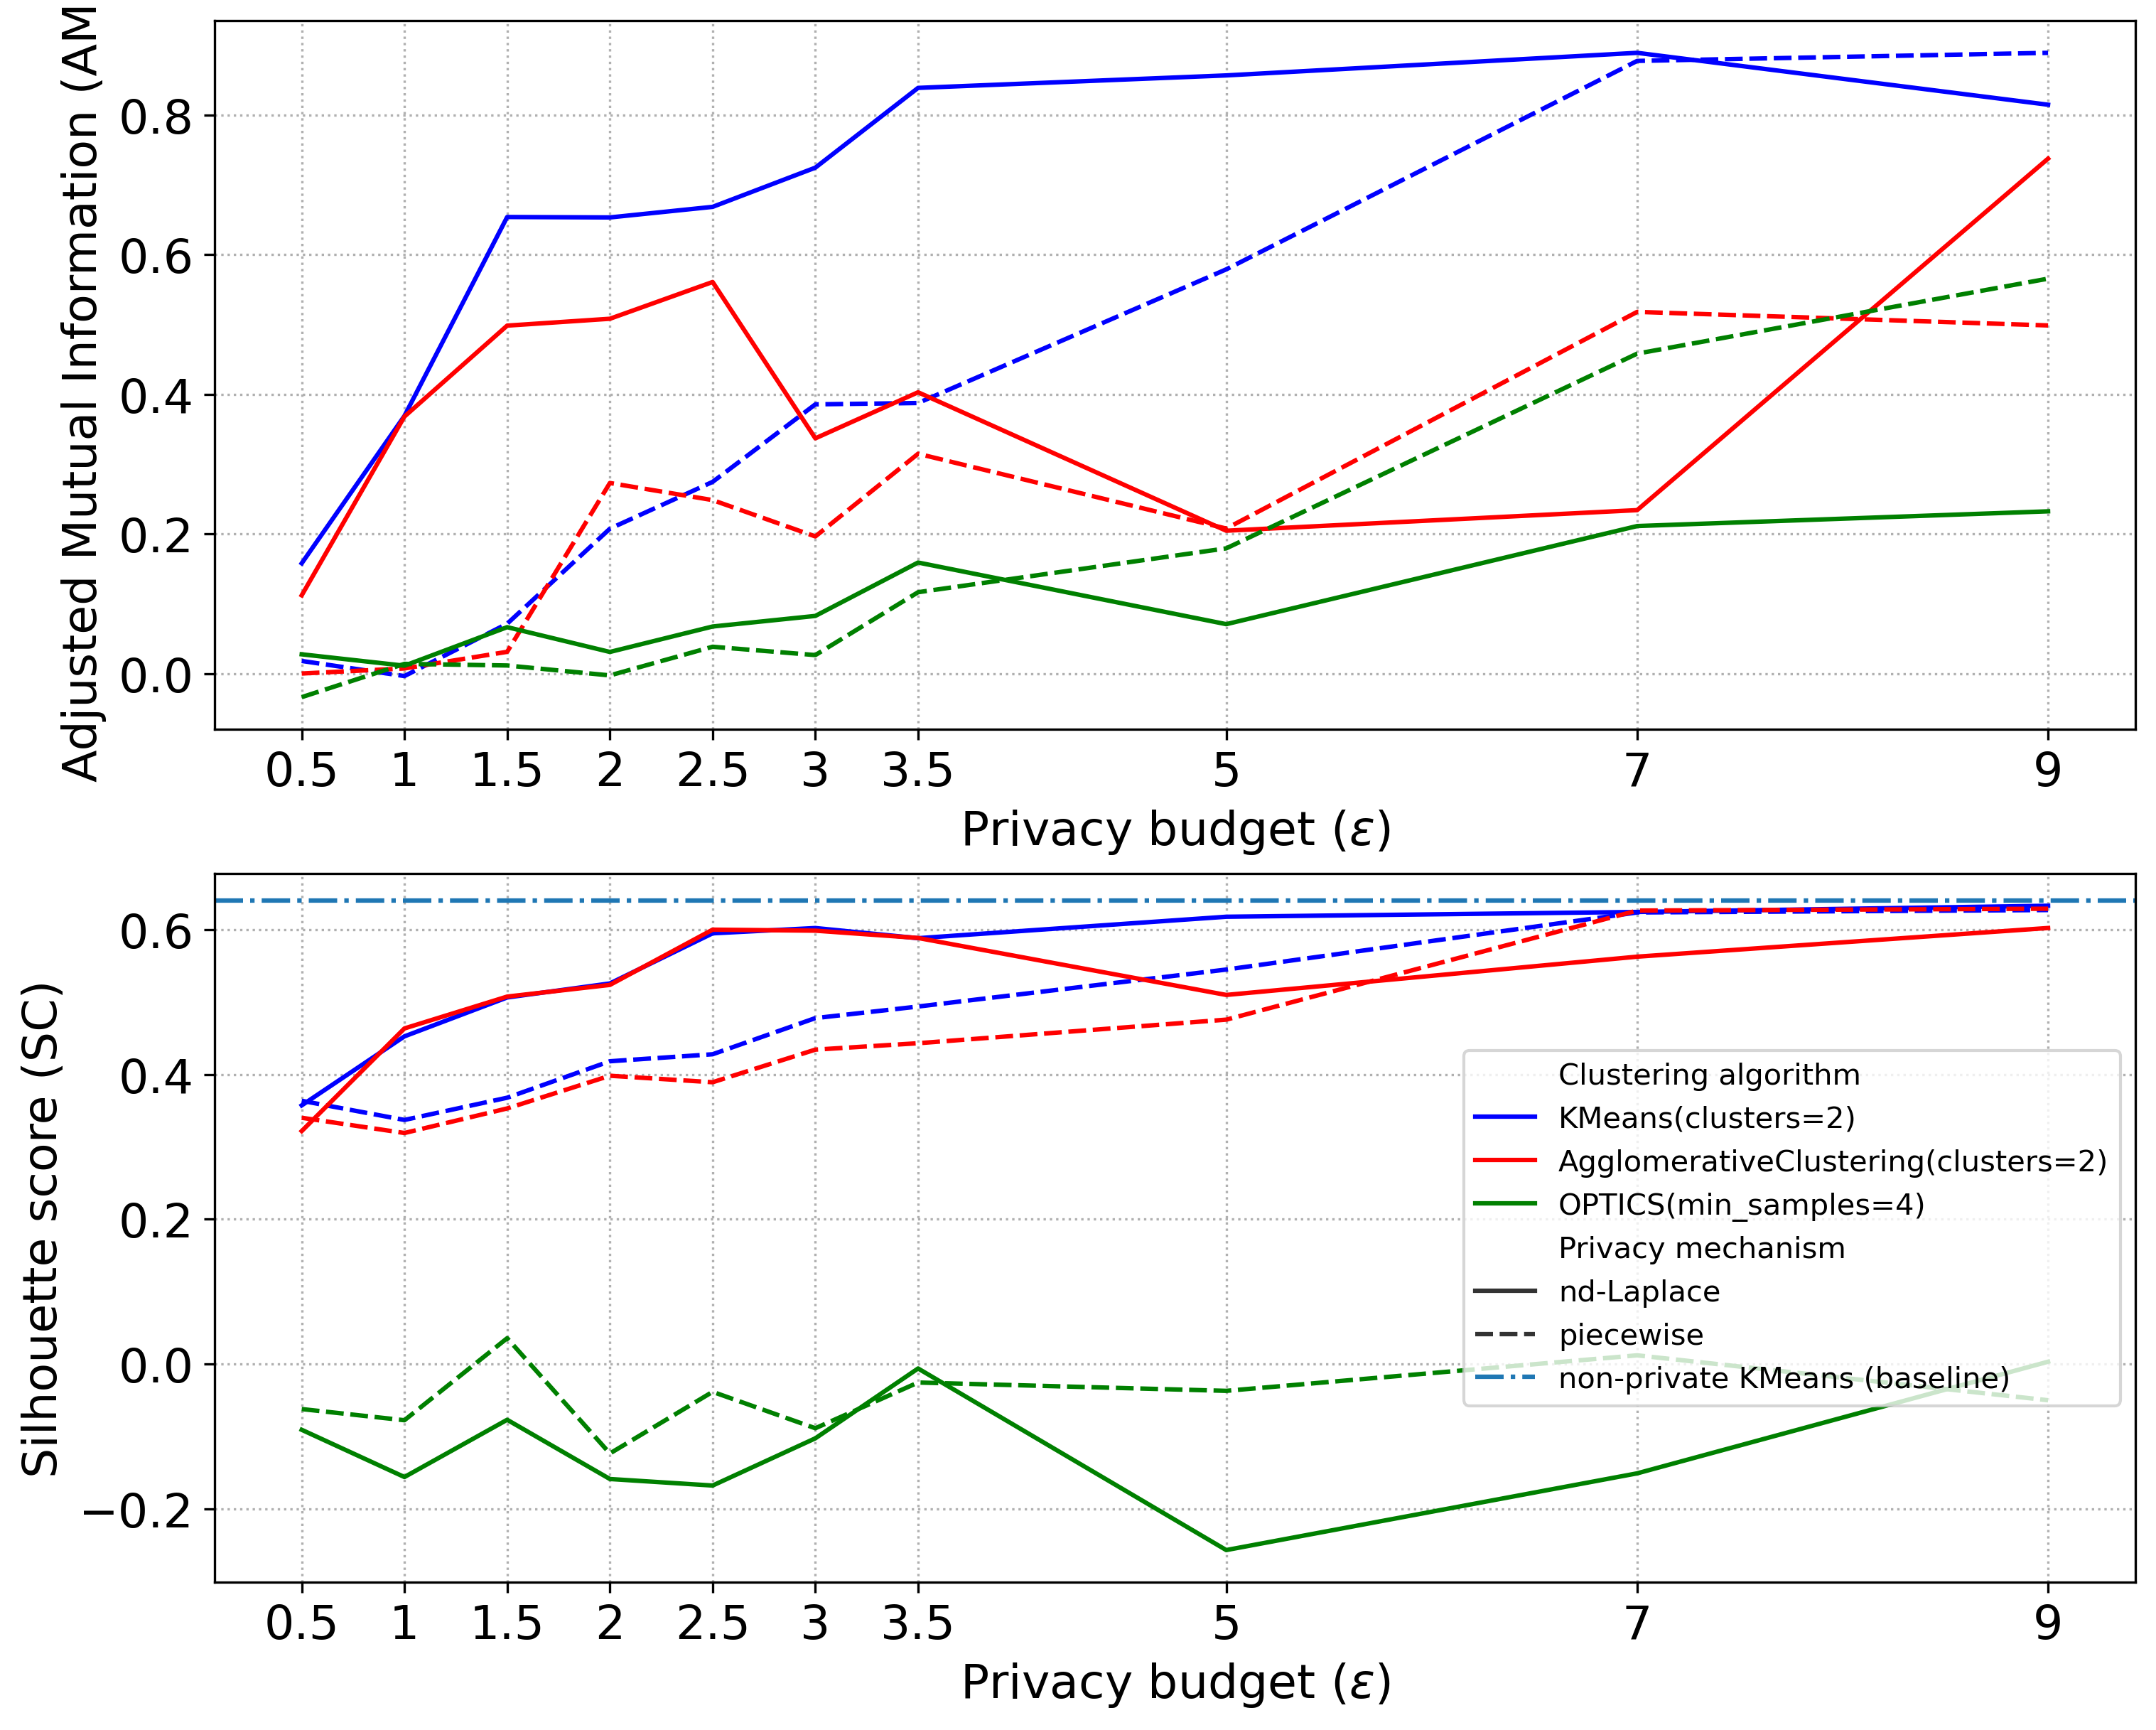
\includegraphics[width=0.8\textwidth]{Results/nd-laplace/nd-Laplace/seeds-dataset/ami-and-sc_2_dimensions.png}

  \label{fig:validation-seeds-dataset_comparison_2d-laplace}
\end{figure}
%The above plots show the AMI and ARI scores for the seeds-dataset with kd-laplace/grid/optimal (left-side) and piecewise (right-side).
The Piecewise mechanism excels in Adjusted Mutual Information (\gls{ami}) at a privacy budget (epsilon) of 9, while the nd-Laplace mechanism is superior for other epsilon values. K-Means consistently outperforms other clustering algorithms, though only marginally over \gls{ag}, and both yield similar silhouette coefficient (\gls{sc}) scores. The underperformance of the OPTICS algorithm across both mechanisms, comparable only to the AP algorithm under Piecewise, suggests its potential limitations in these configurations.
\newpage
The plot shows that nD-Laplace performs better for lower epsilons. Which is likely due to the mechanism also considering the shape (distance) of the data, so the Piecewise mechanism proportionally adds more noise. But, then we would expect OPTICS to score better. Therefore, we visualize this behaviour:
\begin{figure}[H]
    \centering
    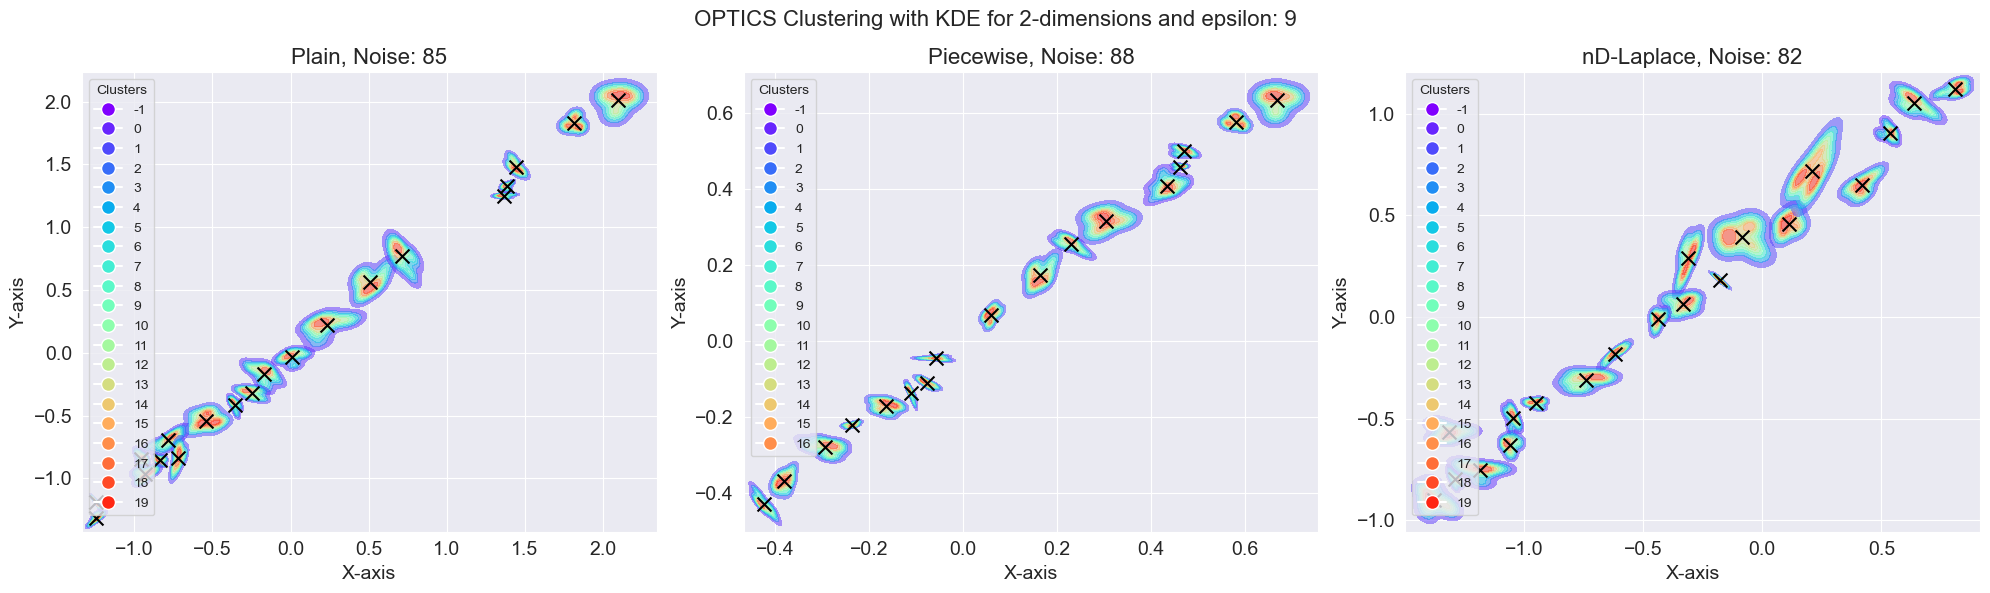
\includegraphics[width=1\linewidth]{Discussion/behaviour-2d-seeds-dataset&optics.png}
    \caption{Evaluating OPTICS for seeds-dataset 2-dimensional data (epsilon 9)}
    \label{fig:evaluate-optics-seeds-dataset-2d-9eps}
\end{figure}
The plot above illustrates the kernel density of core points chosen by the OPTICS algorithm for data with an epsilon value of 9. Clusters within the Plain and Piecewise datasets are compact and exhibit linear alignment, suggesting a distinct data distribution or directional noise stemming from the Piecewise mechanism. Conversely, the nD-Laplace clusters are more scattered, indicating that its noise impacts data uniformly across all directions.

Furthermore, the noise level is concerning. According to Schubert et al. (2017) \citep{schubert_dbscan_2017}, the noise should range between 1\% and 30\%. However, the OPTICS algorithm we employed indicates an average noise level of 40\%, pointing to a potential problem with the algorithm's implementation. Additionally, the number of clusters reported is notably high.


\newpage
\begin{figure}[H]
  \centering
  \caption{\textbf{AMI (top) and SC (bottom) for the nD-Laplace mechanism for the 2-dimensional data heart-dataset}}
  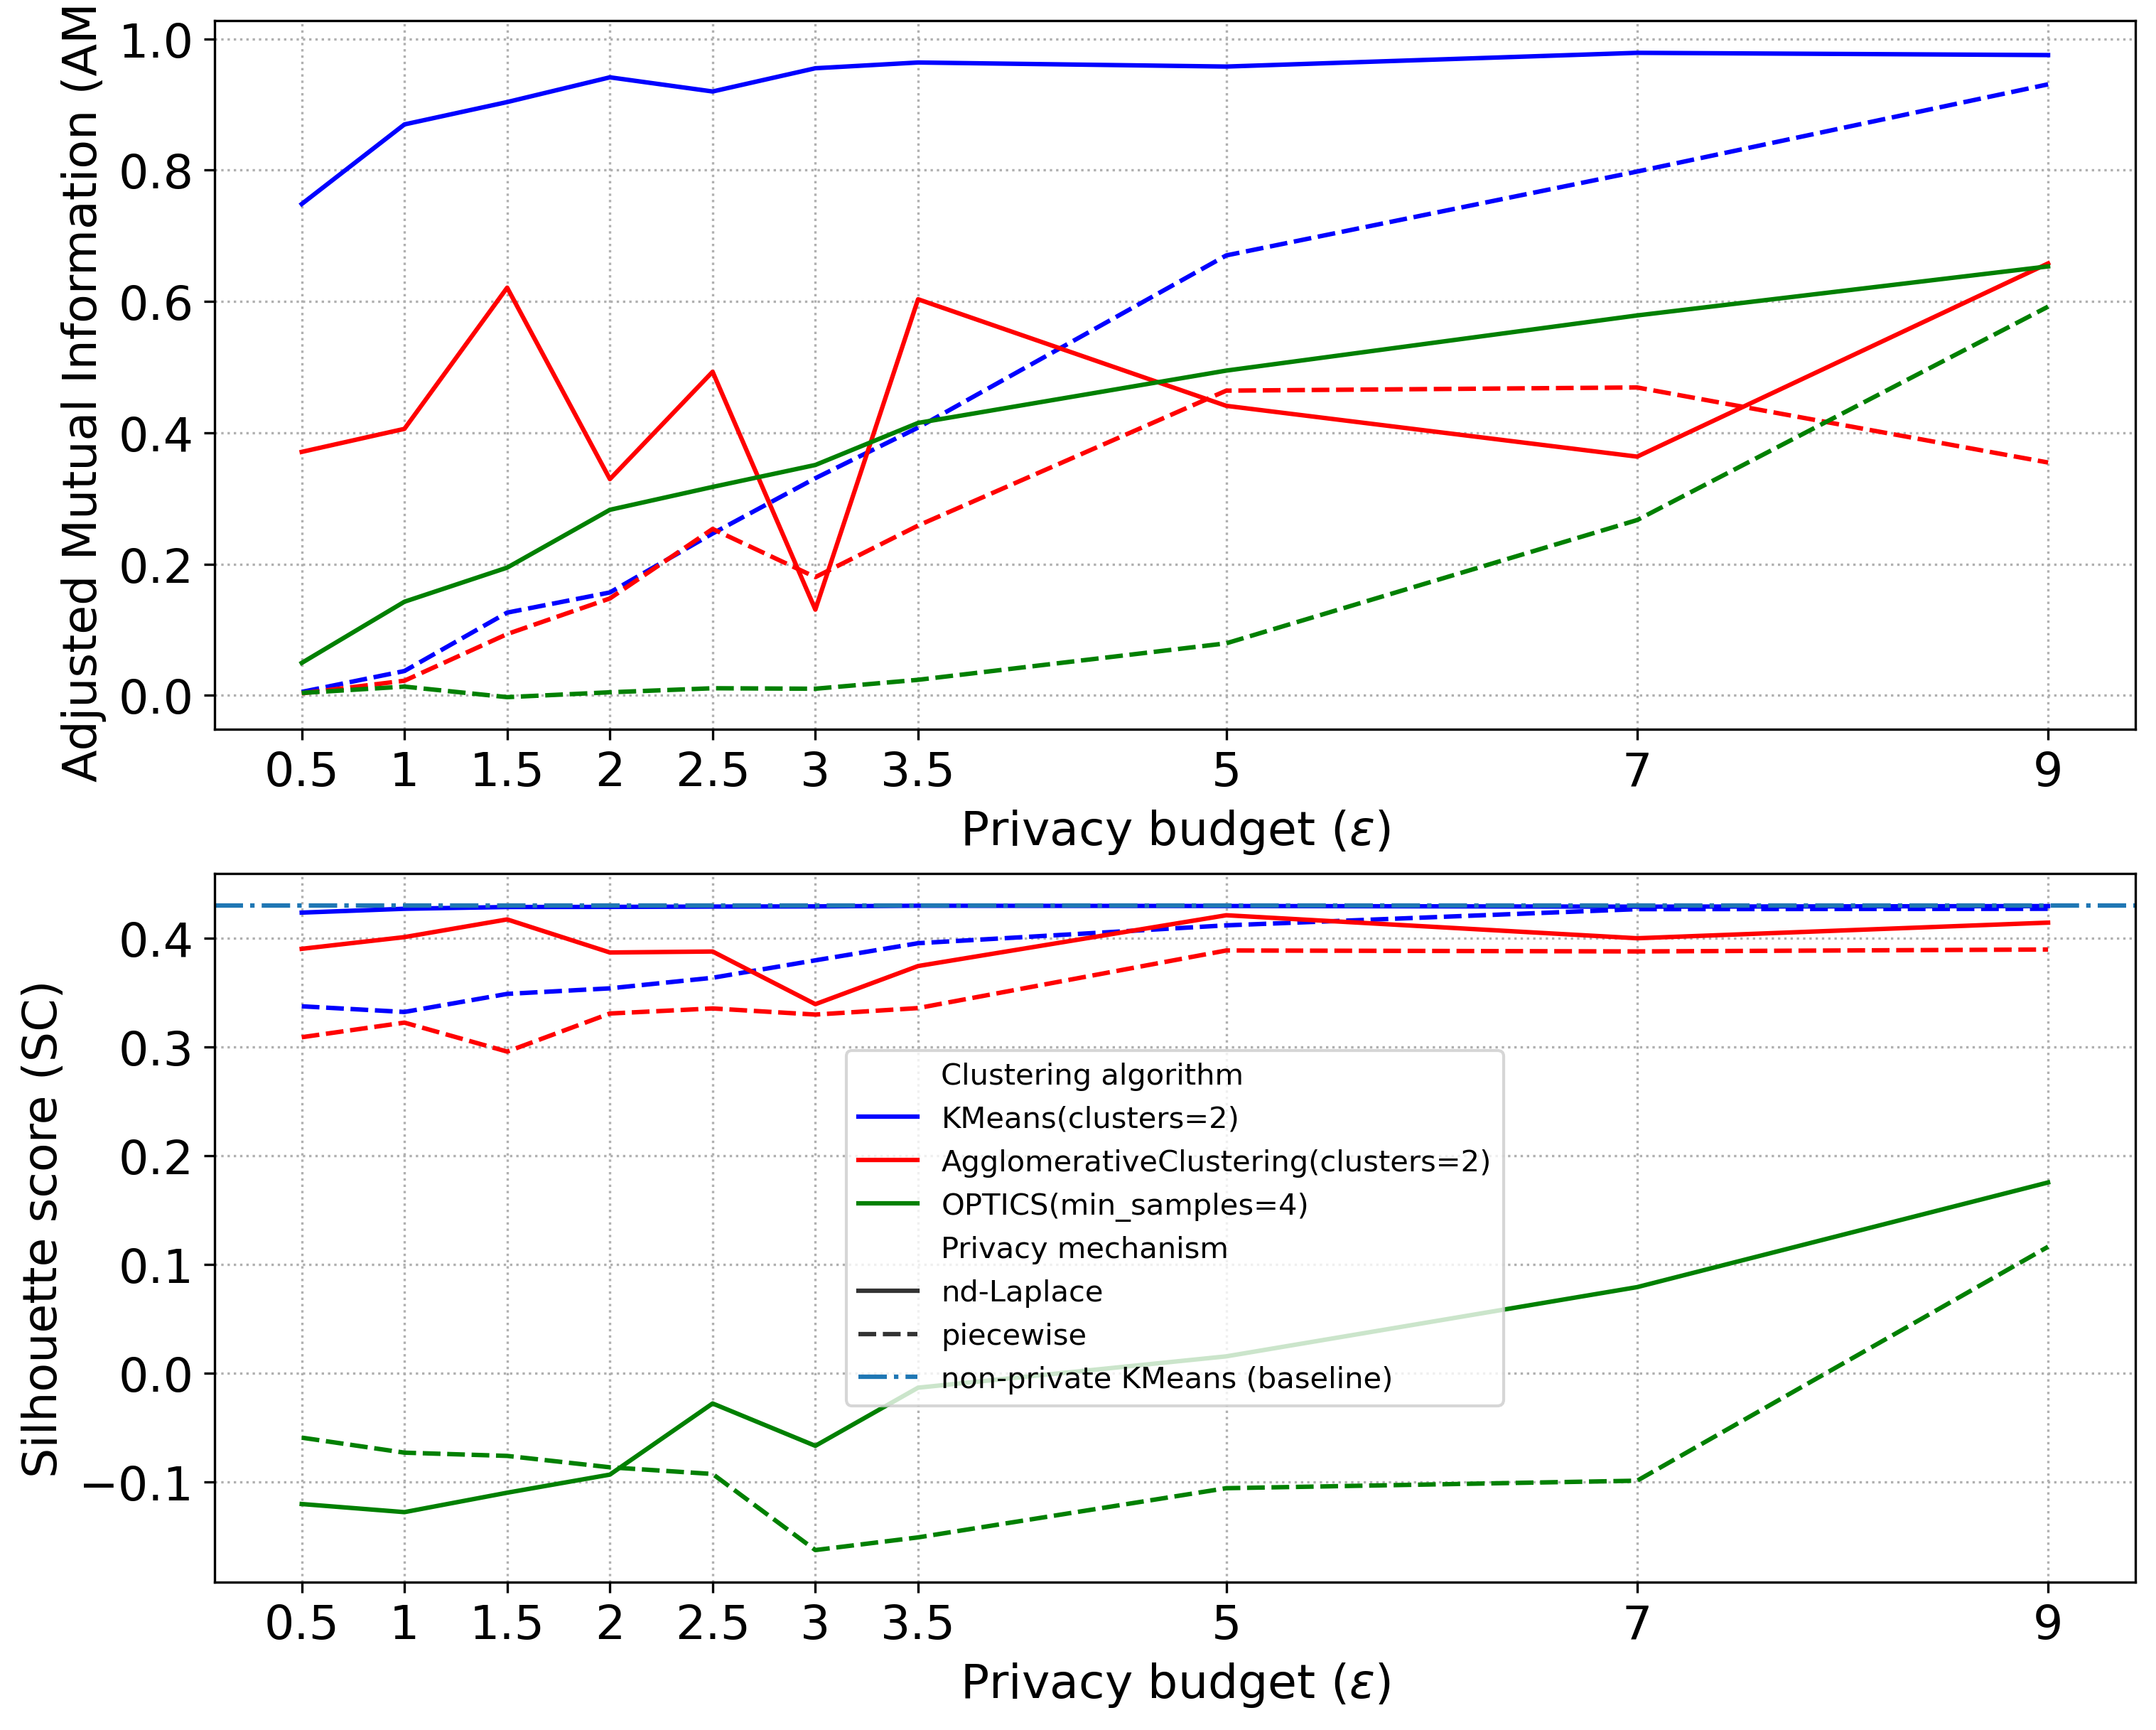
\includegraphics[width=0.9\textwidth]{Results/nd-laplace/nd-Laplace/heart-dataset/ami-and-sc_2_dimensions.png}

  \label{fig:validation-heart-dataset_comparison_2d-laplace}
\end{figure}
Using the K-Means method, the nD-Laplace system works better for all epsilon values. For other methods, the results between the two privacy systems are mostly the same. But, nD-Laplace often does a bit better in \gls{ami} scores. If we compare \gls{optics} with the previous section, we see large improvements. 
When looking at \gls{sc}, both the grouped and K-Means methods do the best for both privacy systems. This is true for most methods. This \gls{ami} score trend matches what we saw with the OPTICS method earlier.

The trends observed in these charts closely mirror those from the seeds-dataset. However, the outcomes here are more consistent. Remarkably, OPTICS stands out in its performance. This can be attributed to the data's configuration. As depicted in Figure \ref{fig:evaluate-optics-seeds-dataset-2d-9eps}, there's a pronounced spread in the nD-Laplace data, similar to the heart-dataset. When data is inherently well-separated, nD-Laplace excels, explaining the strong performance of both Agglomerative and K-Means clustering. This observation is further supported by the \gls{sc}, which aligns closely with the baseline score of K-Means.
\newpage
\begin{figure}[H]
  \centering
  \caption{\textbf{AMI (top) and SC (bottom) for the kD-Laplace mechanism for the 2-dimensional data circle-dataset}}
  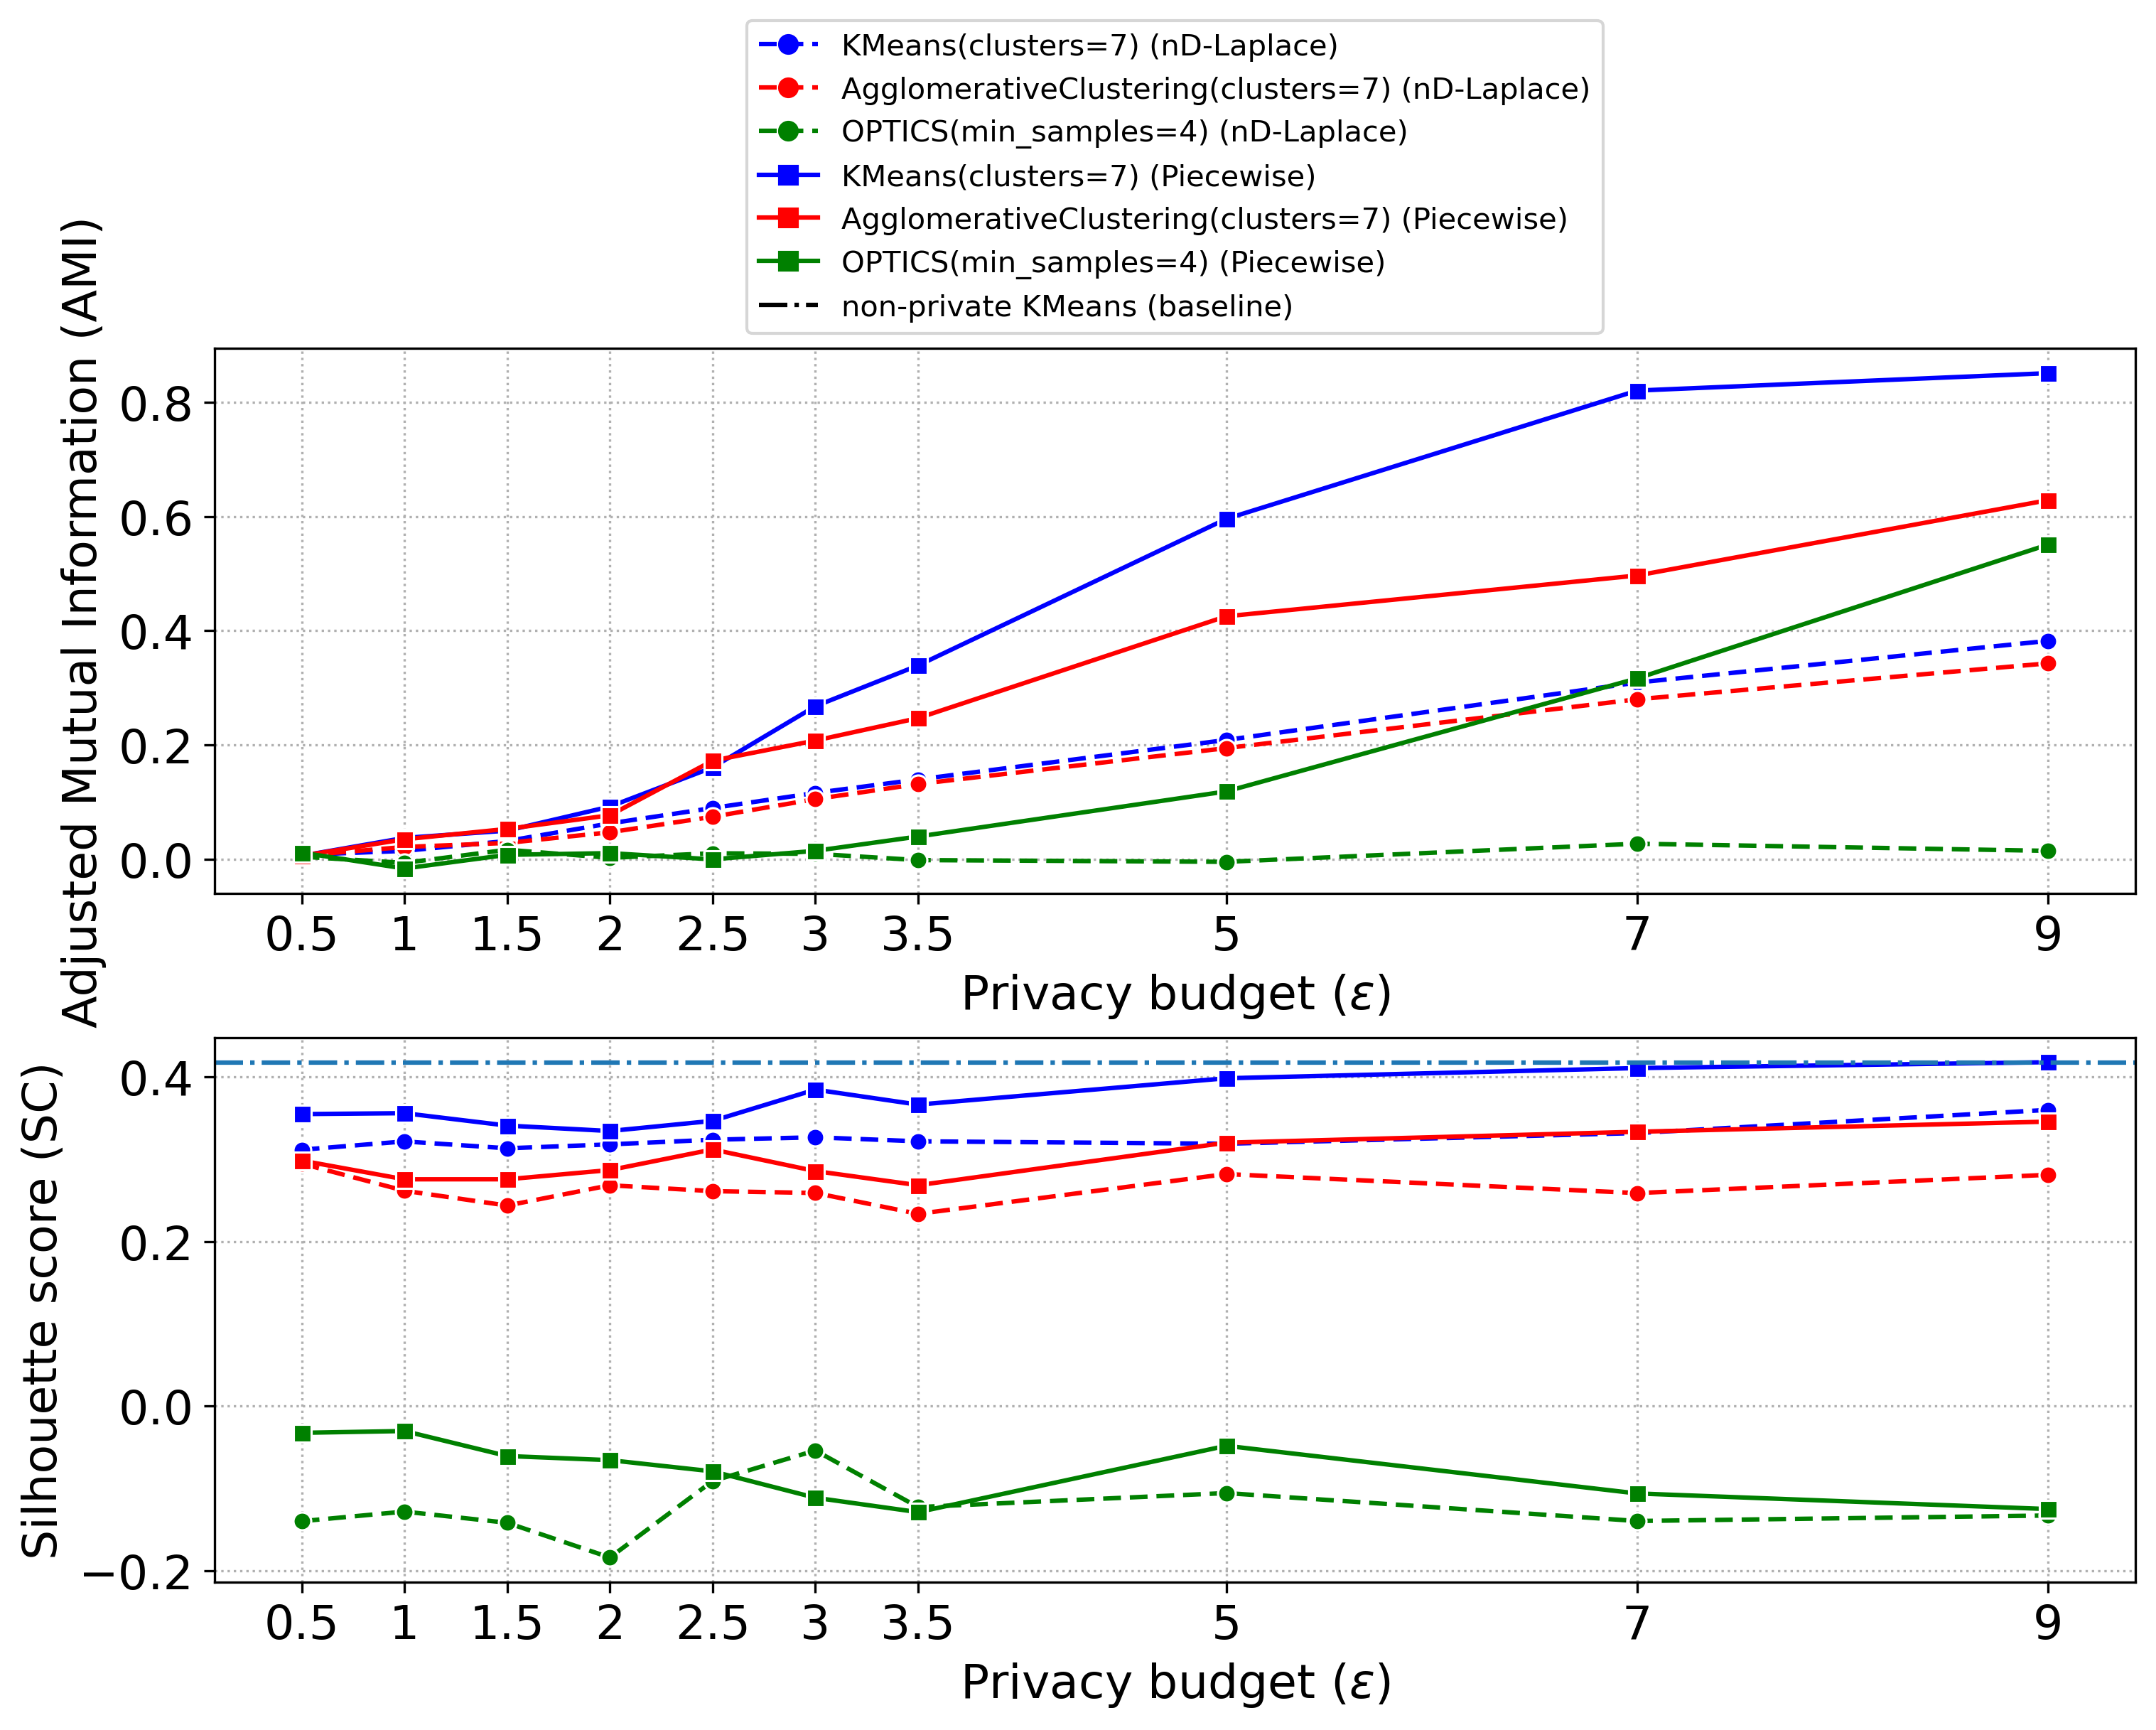
\includegraphics[width=0.9\textwidth]{Results/nd-laplace/nd-Laplace/circle-dataset/ami-and-sc_2_dimensions.png}
  \label{fig:validation-circle-dataset_comparison_2d-laplace}
\end{figure}
Among the two mechanisms, Piecewise consistently achieves the highest scores for all \gls{ami} metrics. Analyzing the three algorithms, a recurring pattern emerges: K-Means leads in performance, trailed by Agglomerative and then \gls{optics}. Notably, within the nD-Laplace mechanism, \gls{optics} significantly lags behind the other algorithms. While a similar trend is observed in the \gls{sc} scores, the disparity between the two mechanisms is less pronounced. Yet, \gls{optics} consistently underperforms across all epsilon values.

We observe the same patterns as with the seeds-dataset; which is shaped as a line.
If there is a thiner line of data, the spread of the data is important. Piecewise mechanism handles this better, to stay close to the original line of data, while nD-Laplace's data is more spread. There are various factors why this issue impacts \gls{optics} the most, but this is probably due to the Euclidean space metric. Here, the distance matters more then similar metrics, and 
\newpage
\begin{figure}[H]
  \centering
  \caption{\textbf{AMI (top) and SC (bottom) for the kD-Laplace and Piecewise mechanisms for the 2-dimensional data line-dataset}}
  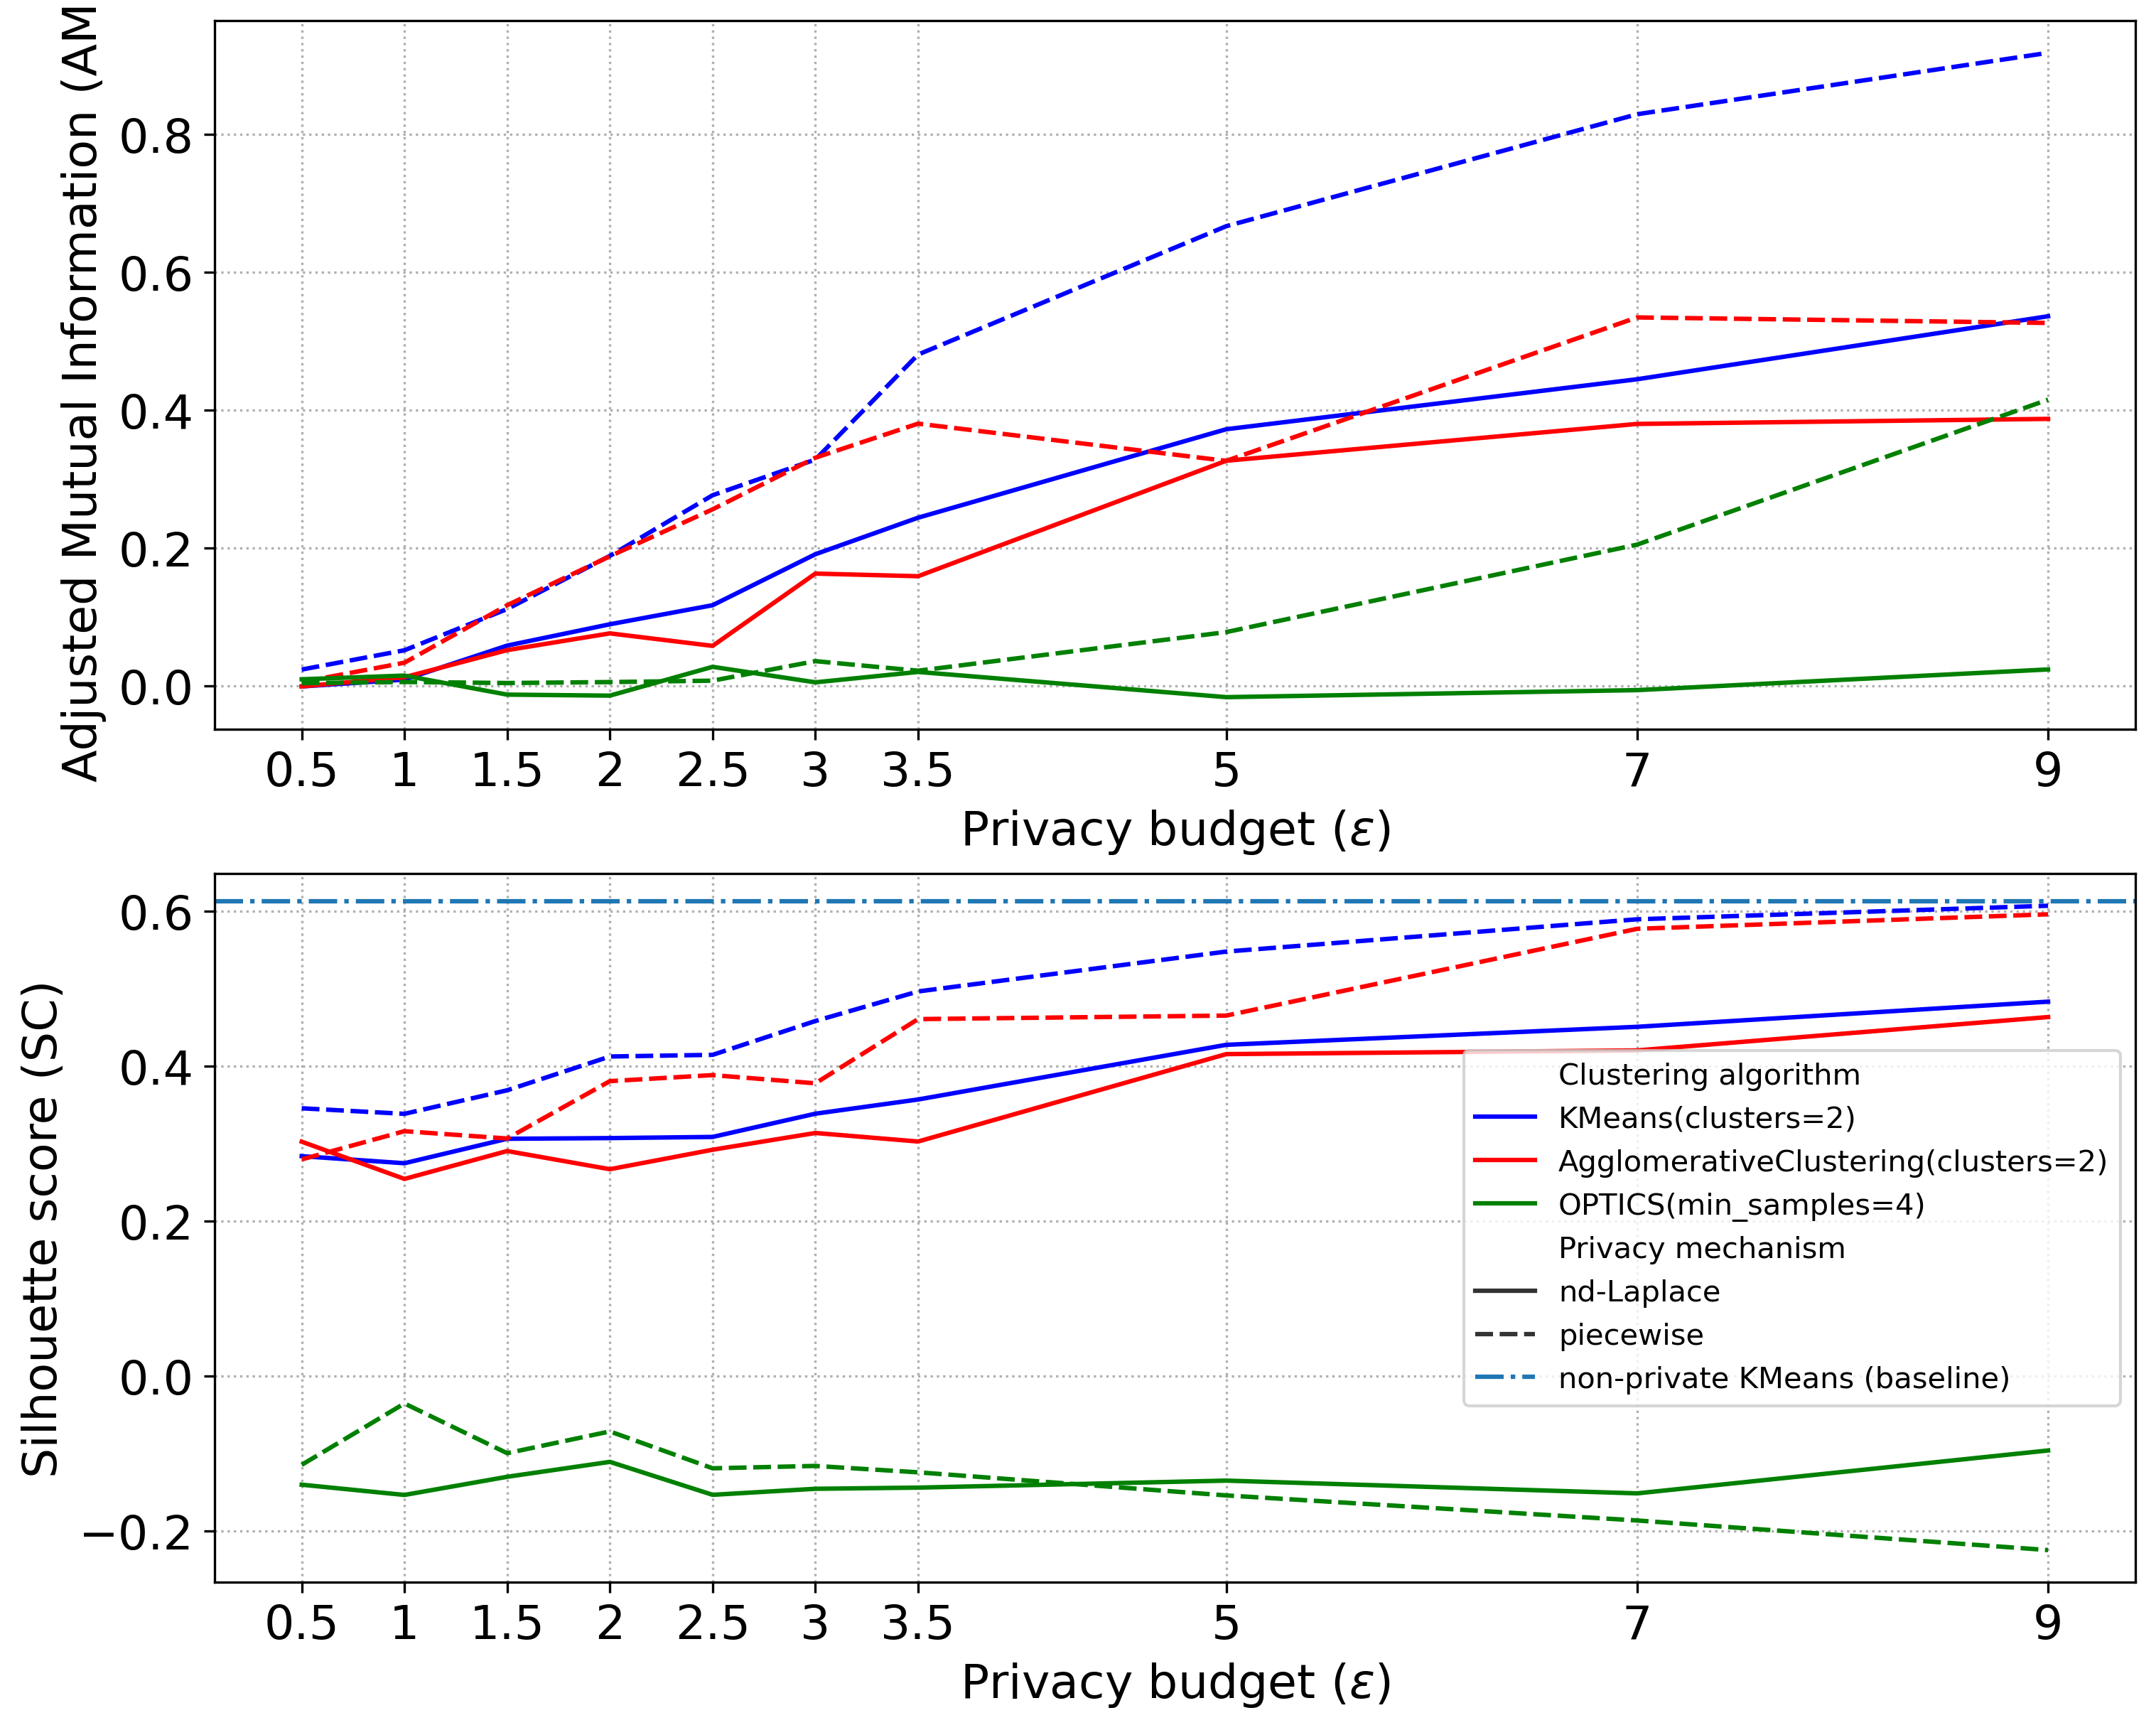
\includegraphics[width=0.9\textwidth]{Results/nd-laplace/nd-Laplace/line-dataset/ami-and-sc_2_dimensions.png}
  \label{fig:validation-line-dataset_comparison_2d-laplace}
\end{figure}
The nD-Laplace algorithm performs best with a privacy budget of 9 for K-Means (\gls{ami} 0.55 - 0.6).
\gls{ag} performs slightly worse with a budget of 9 (\gls{ami} 0.4).
Piecewise outperforms other methods, scoring 0.83 \gls{ami} for K-Means at budget 9 and better for different budgets, .
For \gls{sc}, the mechanisms have similar scores, with Piecewise at baseline from budget 5, kD-Laplace at 7, and \gls{ag} beyond baseline from budget 9. 

Overall, the trends observed with the heart-dataset are not mirrored here. The Piecewise mechanism consistently outperforms nD-Laplace across nearly all privacy budgets. Given that the shapes of the line-dataset and seeds-dataset are expected to be analogous, we further illustrate this with the subsequent plot:

\begin{figure}[H]
\centering
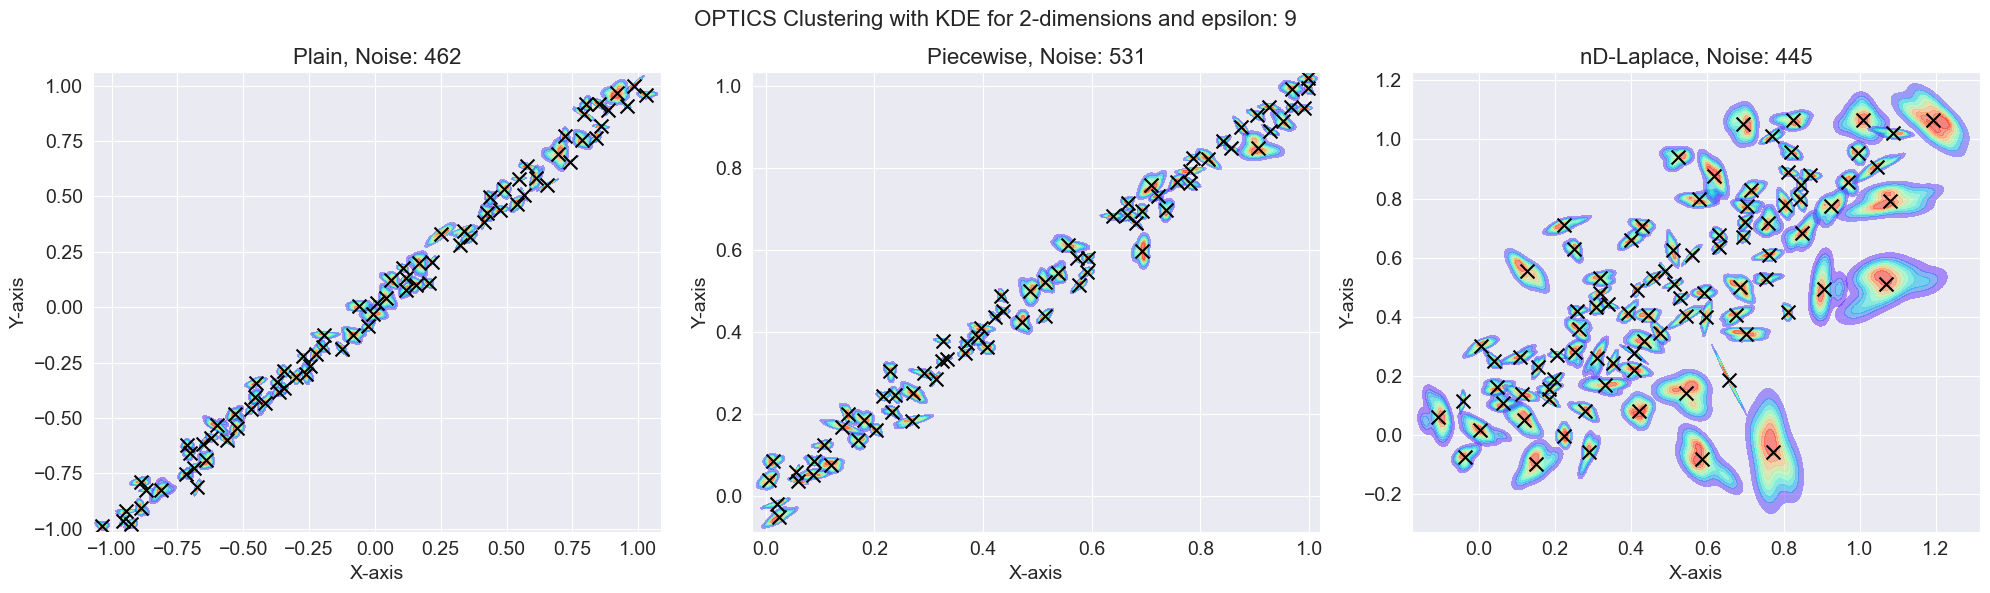
\includegraphics[width=1\linewidth]{Discussion/behaviour-2d-line-dataset&optics.png}
\caption{Evaluating OPTICS and density of points for 2-dimensional Line dataset with epsilon 9}
\label{fig:validation-Line-dataset_comparison_2d-laplace}
\end{figure}

The plot above displays the \gls{optics} scores, denoted by black markers. Even though the data bears resemblance to the seeds-dataset, the dispersion is significantly greater for the nD-Laplace mechanism. This can be attributed to the line shape of the data, as the nD-Laplace mechanism disperses noise uniformly in all directions. However, the extent of this dispersion is notably greater than that observed in the seeds-dataset, leading to inferior results.
\todo[inline]{Analyze why this is such a big difference}

\newpage
\begin{figure}[H]
  \centering
  \caption{\textbf{AMI (top) and SC (bottom) for the kD-Laplace and Piecewise mechanisms for the 2-dimensional data skewed-dataset}}
  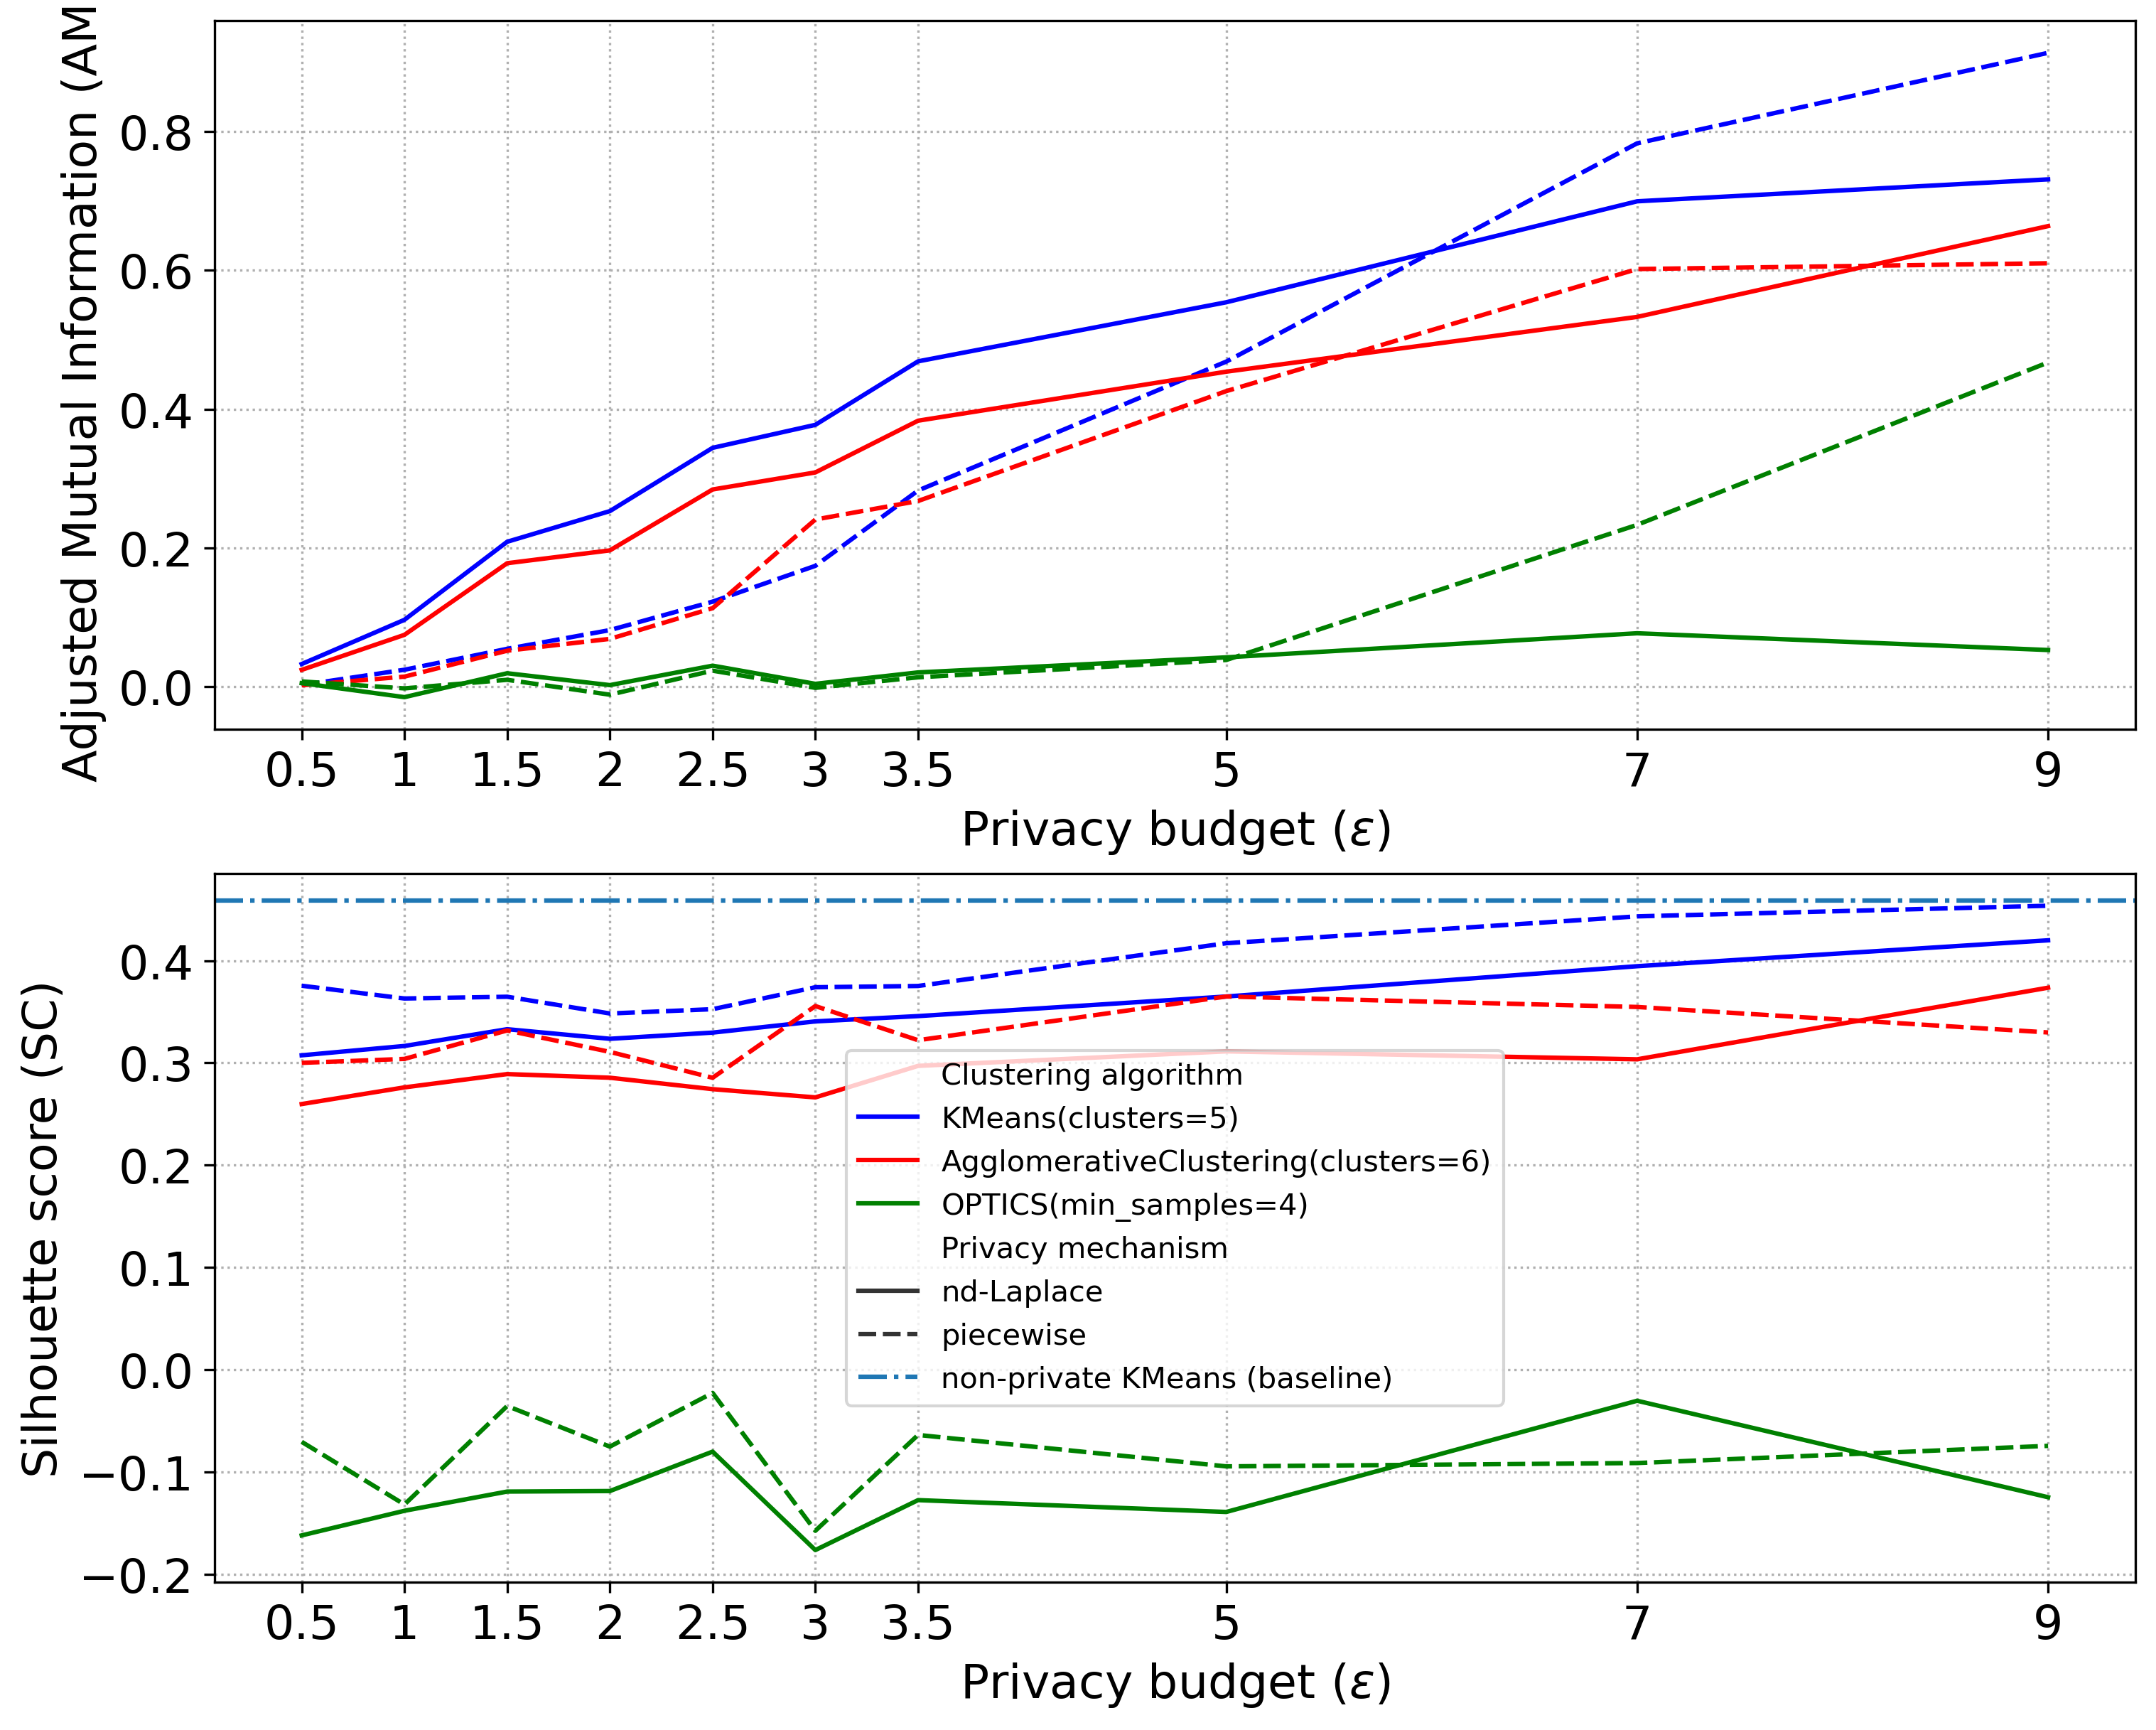
\includegraphics[width=0.9\textwidth]{Results/nd-laplace/nd-Laplace/skewed-dataset/ami-and-sc_2_dimensions.png}
  \label{fig:validation-skewed-dataset_comparison_2d-laplace}
\end{figure}
In our analysis, the nD-Laplace mechanism exhibits its peak performance when paired with K-Means, achieving an \gls{ami} range of 0.74 to 0.78 at privacy budgets of 7 and 9. Conversely, while Piecewise registers higher scores with K-Means for these specific budgets, it lags behind nD-Laplace for other privacy budgets. When considering the \gls{ag} scores, both mechanisms present comparable results. However, nD-Laplace has a slight edge, particularly at lower privacy budgets. This trend of nD-Laplace's superiority at reduced privacy budgets is consistent across different algorithms. A recurring observation is the under performance of \gls{optics}, although it still manages to score 0.43 at a privacy budget of 9 when using the Piecewise mechanism. As for the \gls{sc} metric, the patterns remain consistent: K-Means emerges as the top performer for both mechanisms, while \gls{optics} records notably low scores, even dipping below 0.0 for both mechanisms.

\newpage
\subsection{3-dimensional data}
\begin{figure}[H]
  \centering
  \caption{\textbf{AMI (top) and SC (bottom) for the kD-Laplace and Piecewse mechanisms for the 3-dimensional data seeds-dataset}}
  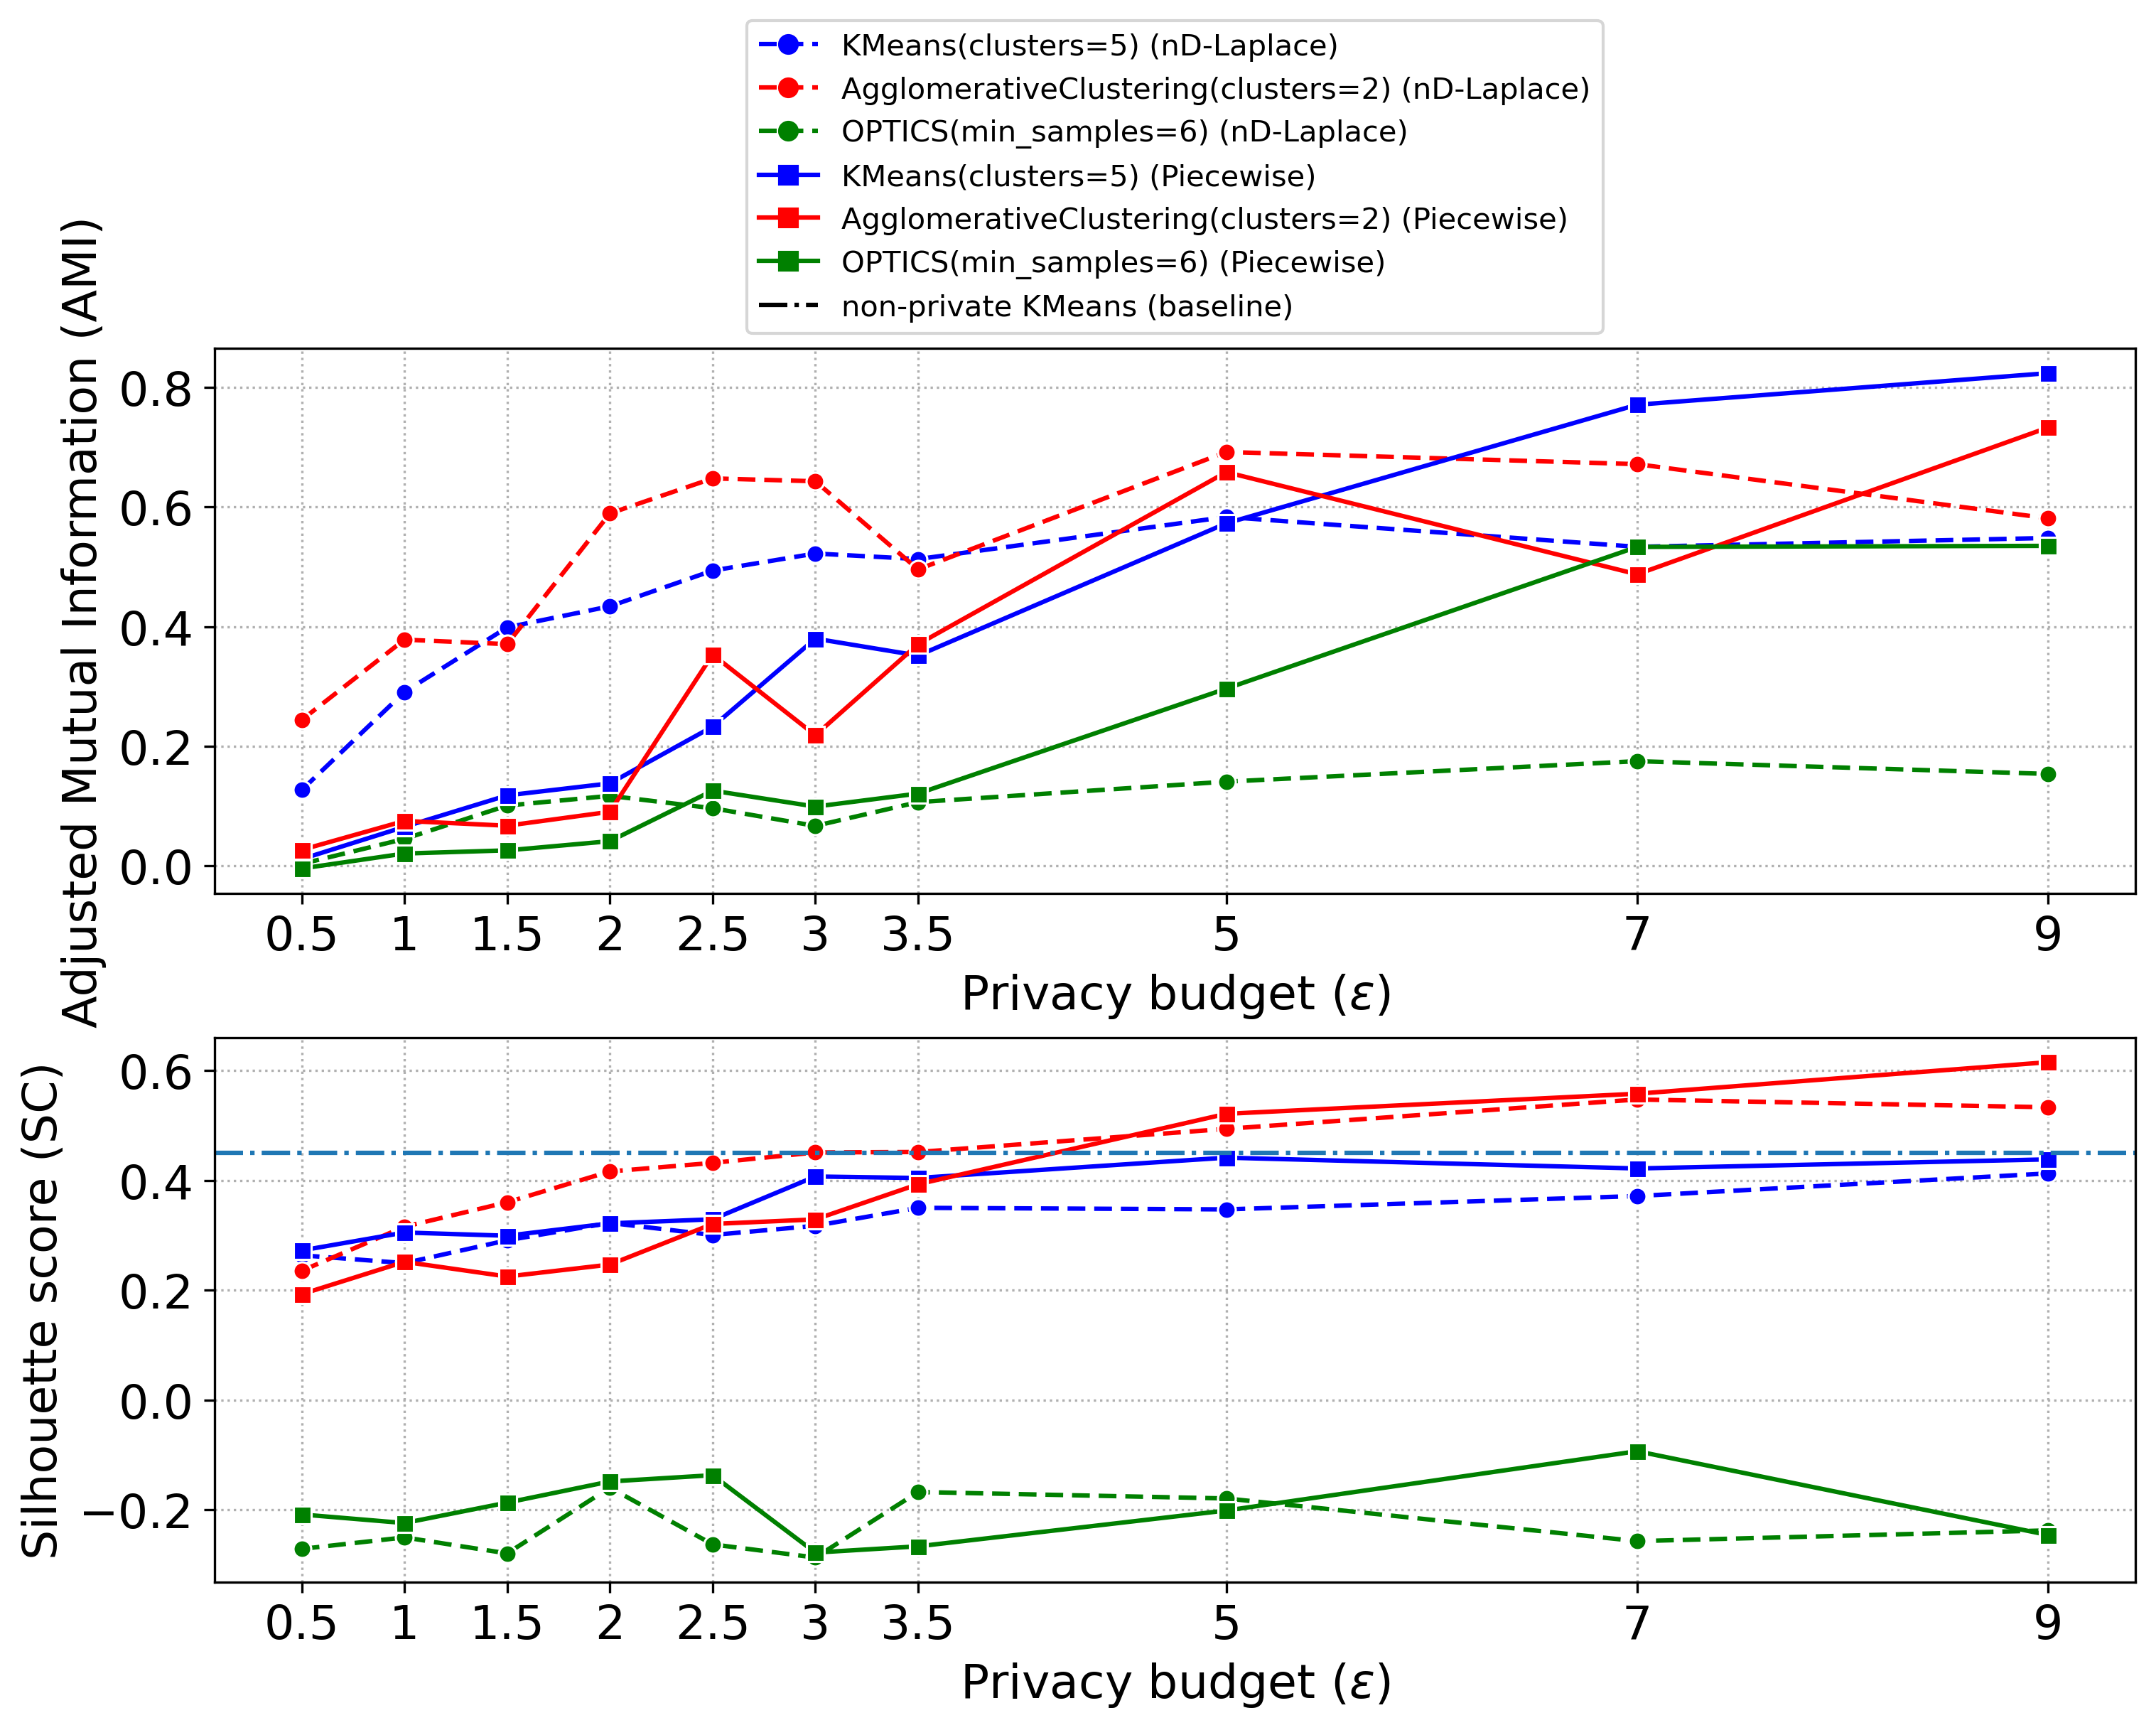
\includegraphics[width=0.9\textwidth]{Results/nd-laplace/nd-Laplace/seeds-dataset/ami-and-sc_3_dimensions.png}
  \label{fig:validation-seeds-dataset_comparison_3d-laplace}
\end{figure}
For the 3-dimensional data, the trend mirrors that observed in the 2-dimensional version of the seeds-dataset. In the range from 0.5 to 5, nD-Laplace outperforms both \gls{ag} and K-Means. Beyond this range, the Piecewise mechanism registers scores approximately 0.10 - 0.20 points higher than nD-Laplace. Conversely, nD-Laplace consistently scores higher for \gls{ag}, with the exception of epsilon 9. Notably, \gls{optics} yields a low score (less than 0.2 \gls{ami}) with nD-Laplace, whereas with Piecewise, the scores range between 0.2 and 0.58 for a privacy budget of 3.5.

For the \gls{sc} metric, the trend is consistent with the \gls{ami} score. However, \gls{ag} achieves a score surpassing the baseline for privacy budgets ranging from 3.5 to 9 across both mechanisms.

In other visual representations, both \gls{ami} and \gls{sc} metrics exhibit comparable trends. Yet, in this specific plot, \gls{ag} is superior to K-Means in performance. While the cluster quality is elevated, it doesn't translate to a higher \gls{ag} score. This suggests that while the mechanisms maintain clusters, they don't necessarily preserve the exact cluster configurations or sizes as observed with the non-private K-Means.

\newpage
\begin{figure}[H]
  \centering

  \caption{\textbf{AMI (top) and SC (bottom) for the kD-Laplace and Piecewise mechanisms for the 3-dimensional data heart-dataset}}
  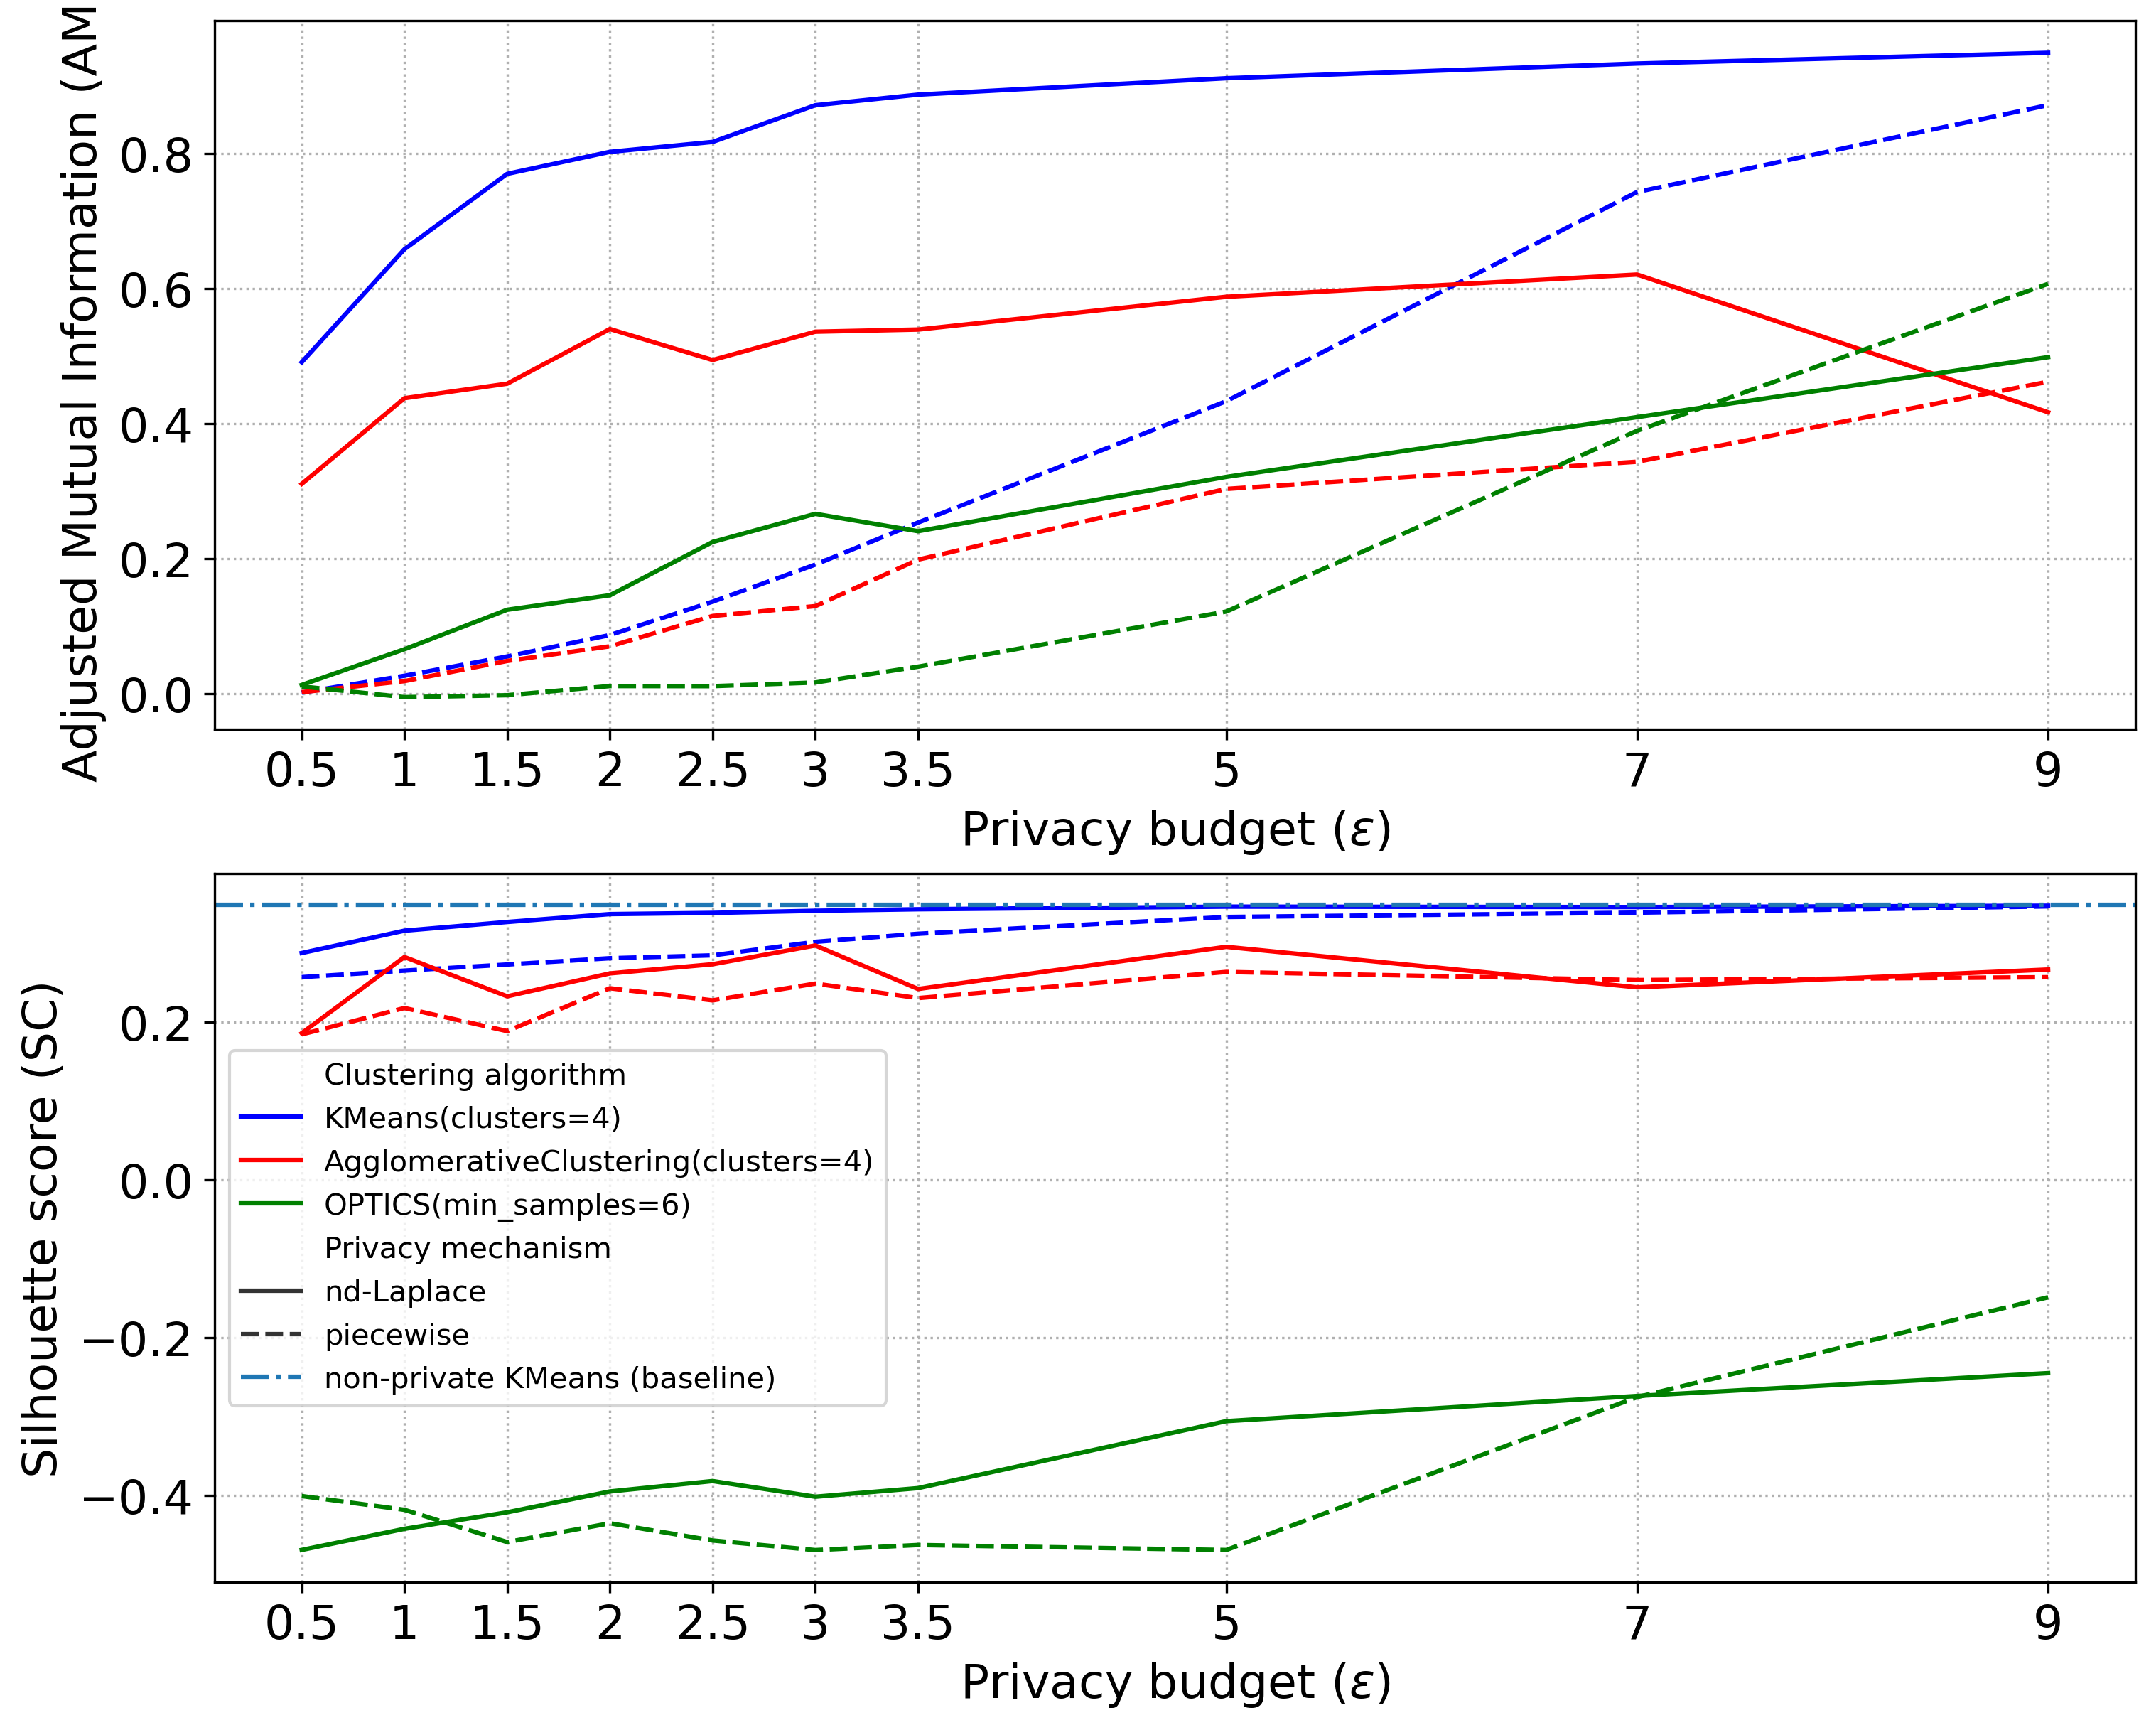
\includegraphics[width=0.9\textwidth]{Results/nd-laplace/nd-Laplace/heart-dataset/ami-and-sc_3_dimensions.png}
  \label{fig:validation-heart-dataset_comparison_3d-laplace}
\end{figure}
The nD-Laplace method gets good results, scoring around +/- 0.87 \gls{ami} for K-Means when the budgets are 7 and 9. This is similar to what we saw with the simpler 2D heart-dataset using the same method. We also noticed that \gls{optics} scores got better compared to other datasets, which matches the results from the 2D heart-dataset. However, \gls{ag} scores a bit lower than K-Means, but the overall pattern is similar.

For the Piecewise method, the scores are below 0.6 \gls{ami} when the budgets are less than 7, but it goes up to 0.8 \gls{ami} for K-Means. When we look at \gls{sc}, both Piecewise and nD-Laplace meet the standard scores for \gls{ag} and K-Means.

Even though \gls{optics} gets high scores for \gls{ami}, it doesn't do as well for \gls{sc}. The main job of \gls{ami} is to compare \gls{optics} to the non-private variant. But if \gls{sc} is low and \gls{ami} is high, it shows that also the non-private has incorrect clusterings.
\newpage
\begin{figure}[H]
  \centering

  \caption{\textbf{AMI (top) and SC (bottom) for the kD-Laplace and Piecewise mechanisms for the 3-dimensional data circle-dataset}}
  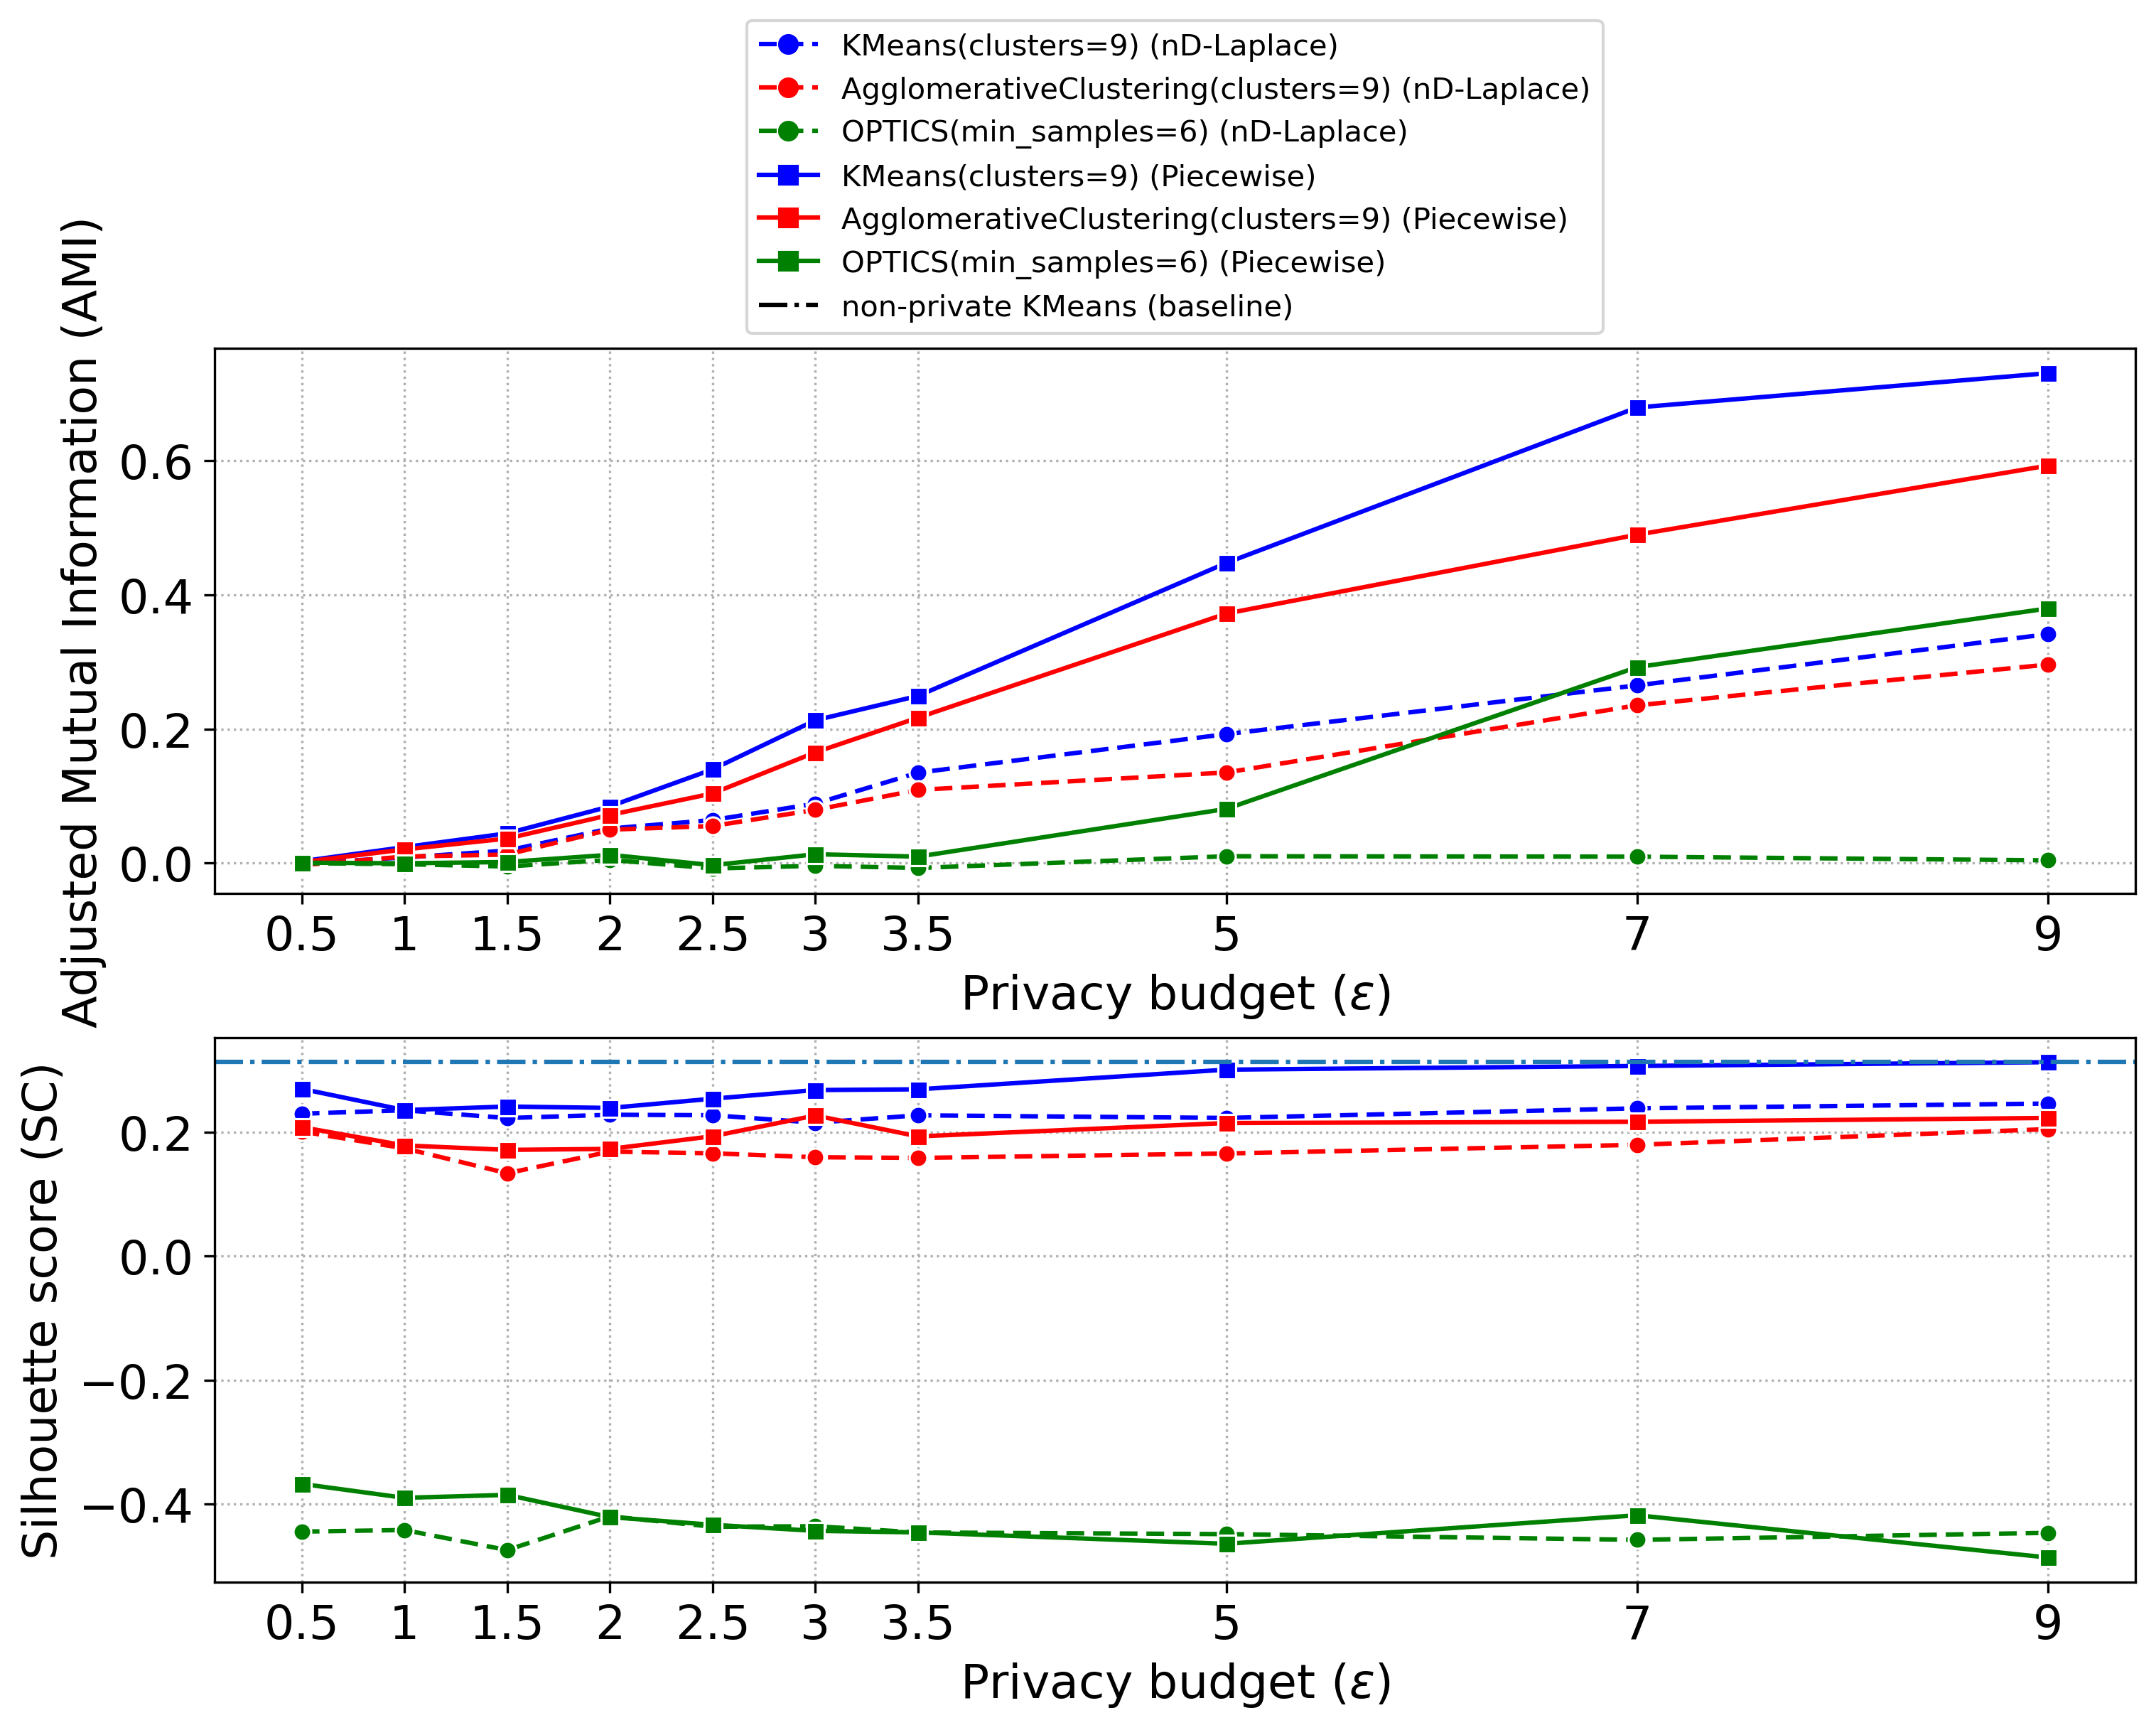
\includegraphics[width=0.9\textwidth]{Results/nd-laplace/nd-Laplace/circle-dataset/ami-and-sc_3_dimensions.png}

  \label{fig:validation-circle-dataset_comparison_3d-laplace}
\end{figure}
The nD-Laplace mechanism excels with K-Means, achieving a peak score of 0.33 \gls{ami}. While \gls{ag} closely follows, \gls{optics} lags significantly with scores less than 0.1 \gls{ami}. Similarly, the Piecewise mechanism registers its highest scores with K-Means, nearing 0.7 \gls{ami}. In this context, \gls{ag} maintains a comparable trend. Notably, \gls{optics} scores higher with Piecewise (less than 0.4 \gls{ami) than with nD-Laplace. For both mechanisms, \gls{sc} scores hover around the baseline at approximately 0.2. Across all privacy budgets, \gls{optics} consistently scores below 0 for \gls{sc}.
\todo[inline]{Discussion}
\newpage
\begin{figure}[H]
  \centering

  \caption{\textbf{AMI (top) and SC (bottom) for the kD-Laplace and Piecewise mechanisms for the 3-dimensional data line-dataset}}
  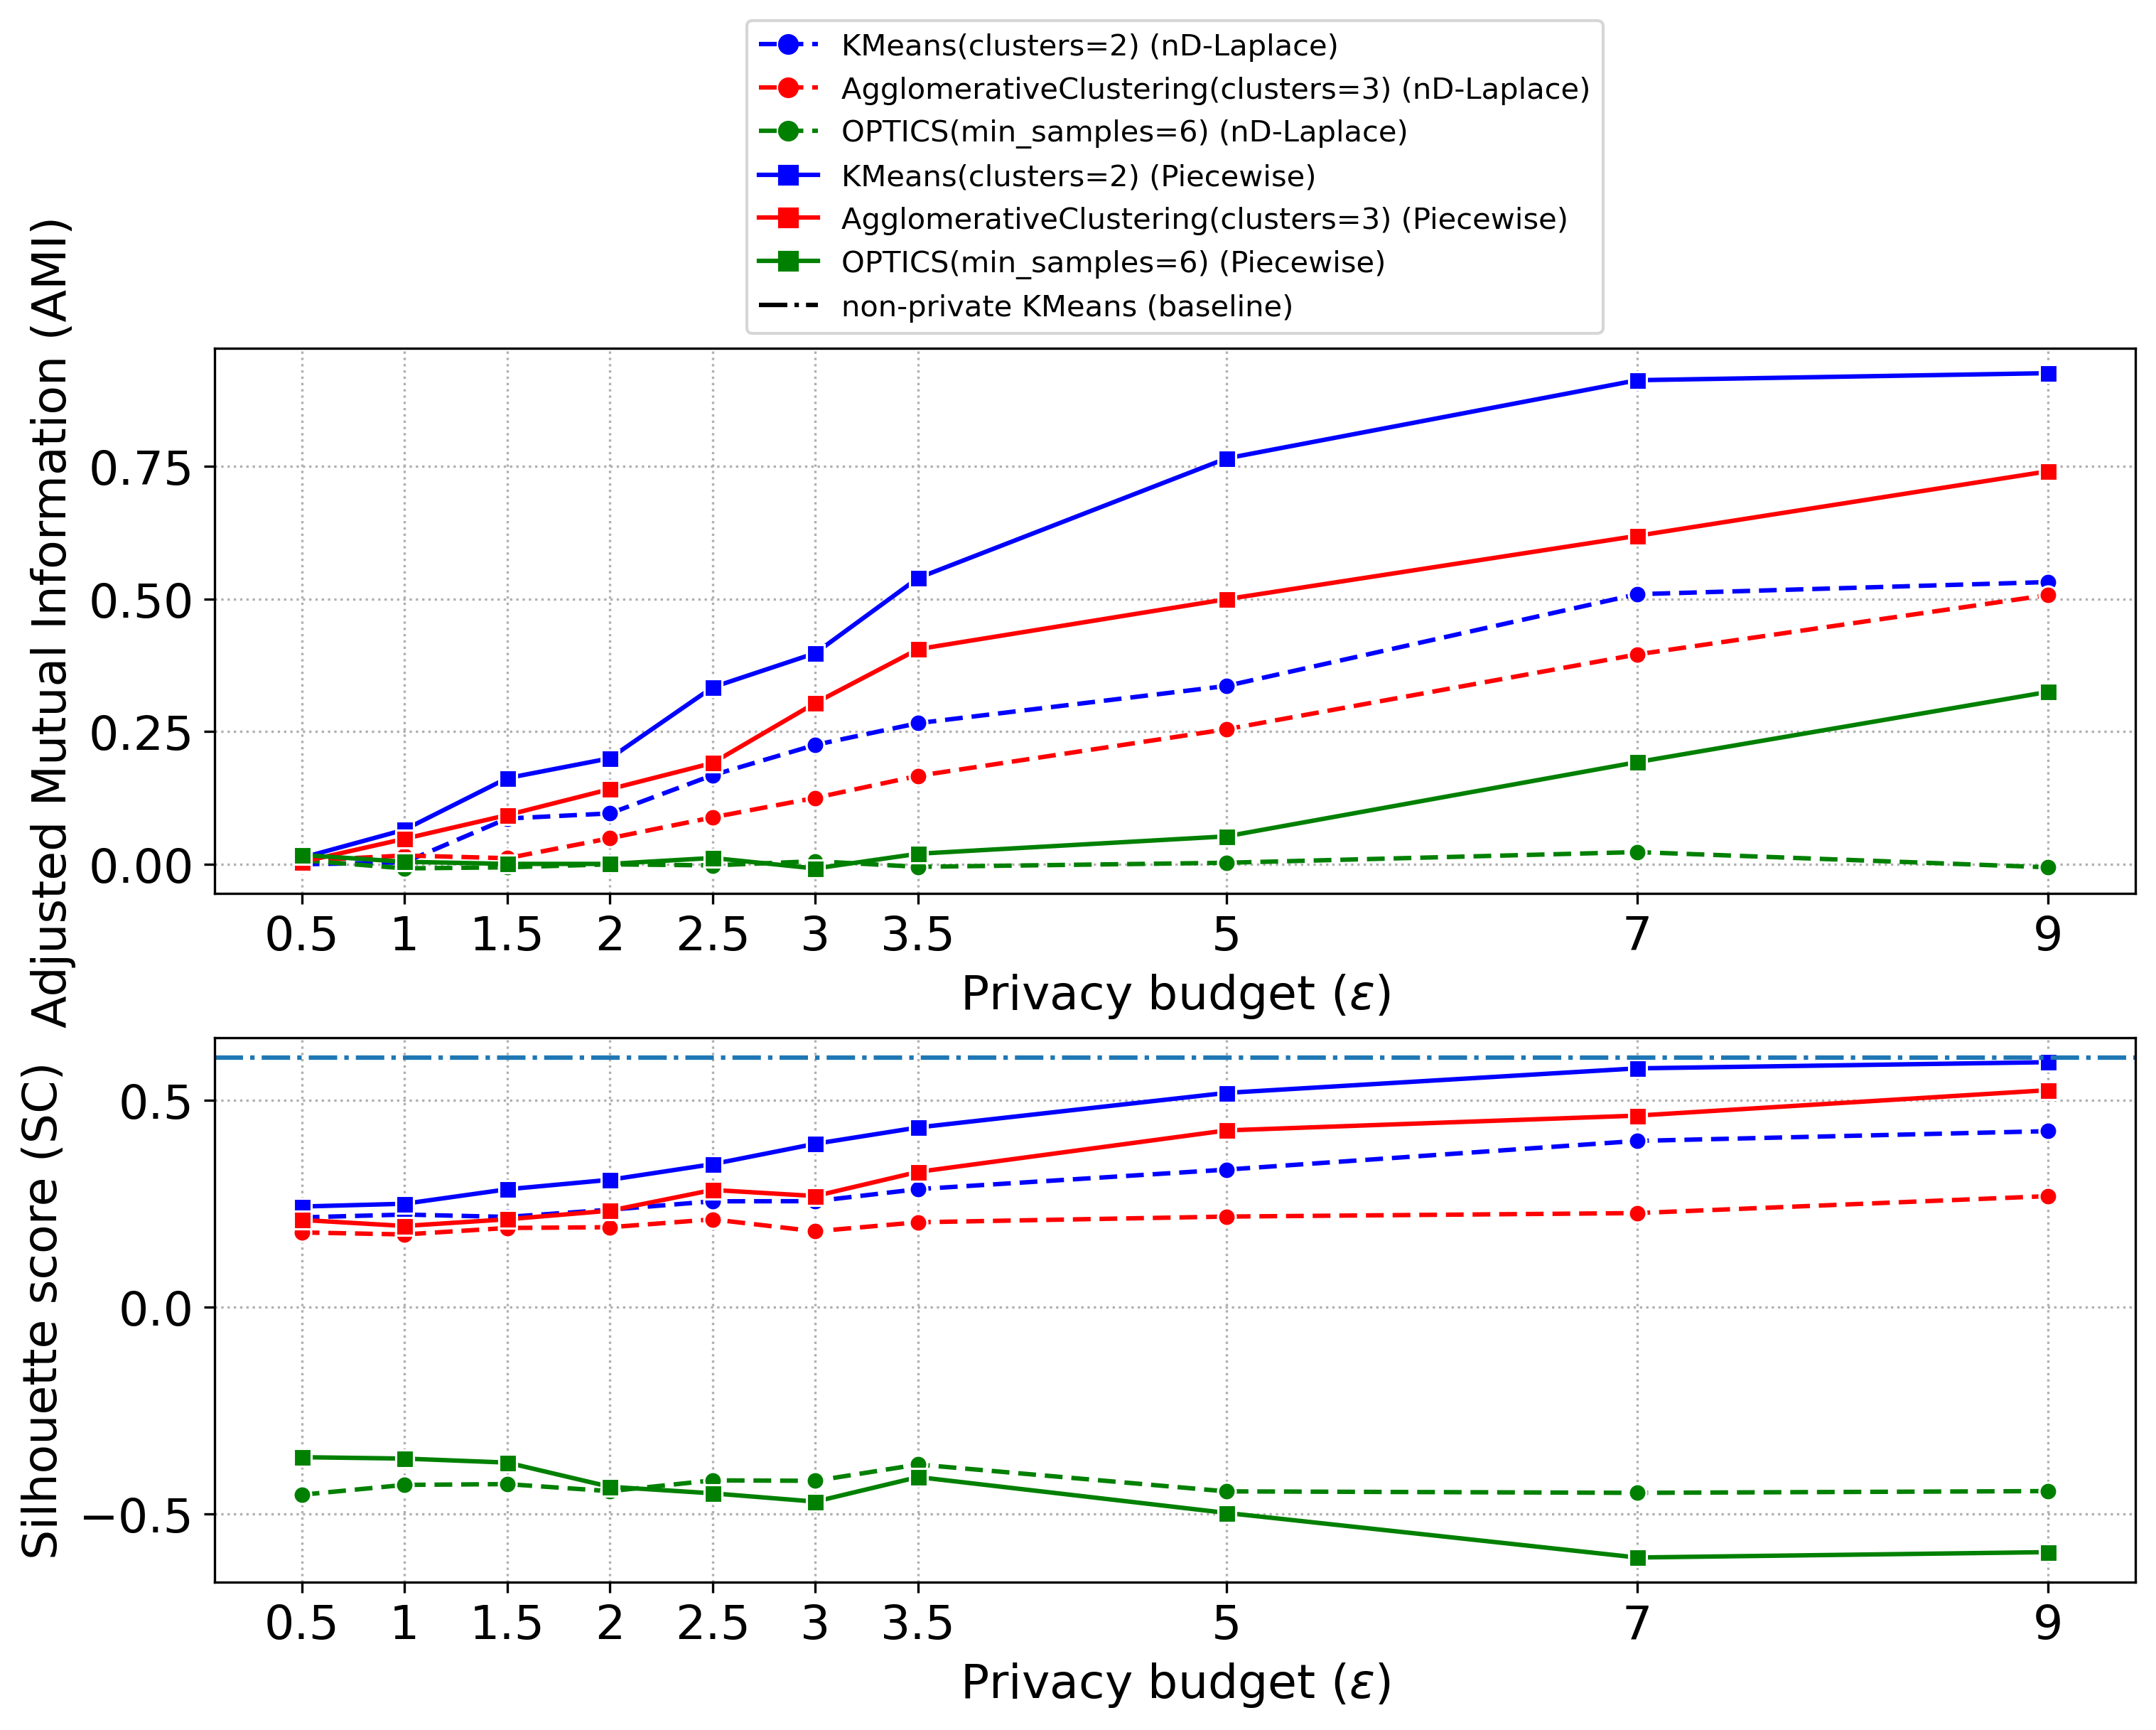
\includegraphics[width=0.9\textwidth]{Results/nd-laplace/nd-Laplace/line-dataset/ami-and-sc_3_dimensions.png}
  \label{fig:validation-line-dataset_comparison_3d-laplace}
\end{figure}
The scores in this plot closely resemble those from the previous one. With nD-Laplace, both K-Means and \gls{ag} lead the pack, though neither surpasses 0.6 \gls{ami}. Notably, \gls{optics} doesn't score at all.

The Piecewise mechanism outperforms nD-Laplace, reaching 0.86 \gls{ami} for privacy budgets at levels 7 and 9. In this scenario, \gls{ag} follows but with notably lower scores: 0.6 and 0.78 \gls{ami} for epsilon 7 and 9, respectively. While \gls{optics} remains a weaker performer across both mechanisms, it does exhibit a positive trajectory with the Piecewise mechanism.

Comparing these findings to the prior set, there are subtle variations in the \gls{sc} metric. Specifically, K-Means and \gls{ag} display a broader range of results, spanning from 0.2 to 0.6.

\newpage
\begin{figure}[H]
  \centering

  \caption{\textbf{AMI (top) and SC (bottom) for the kD-Laplace and Piecewise mechanisms for the 3-dimensional data skewed-dataset}}
  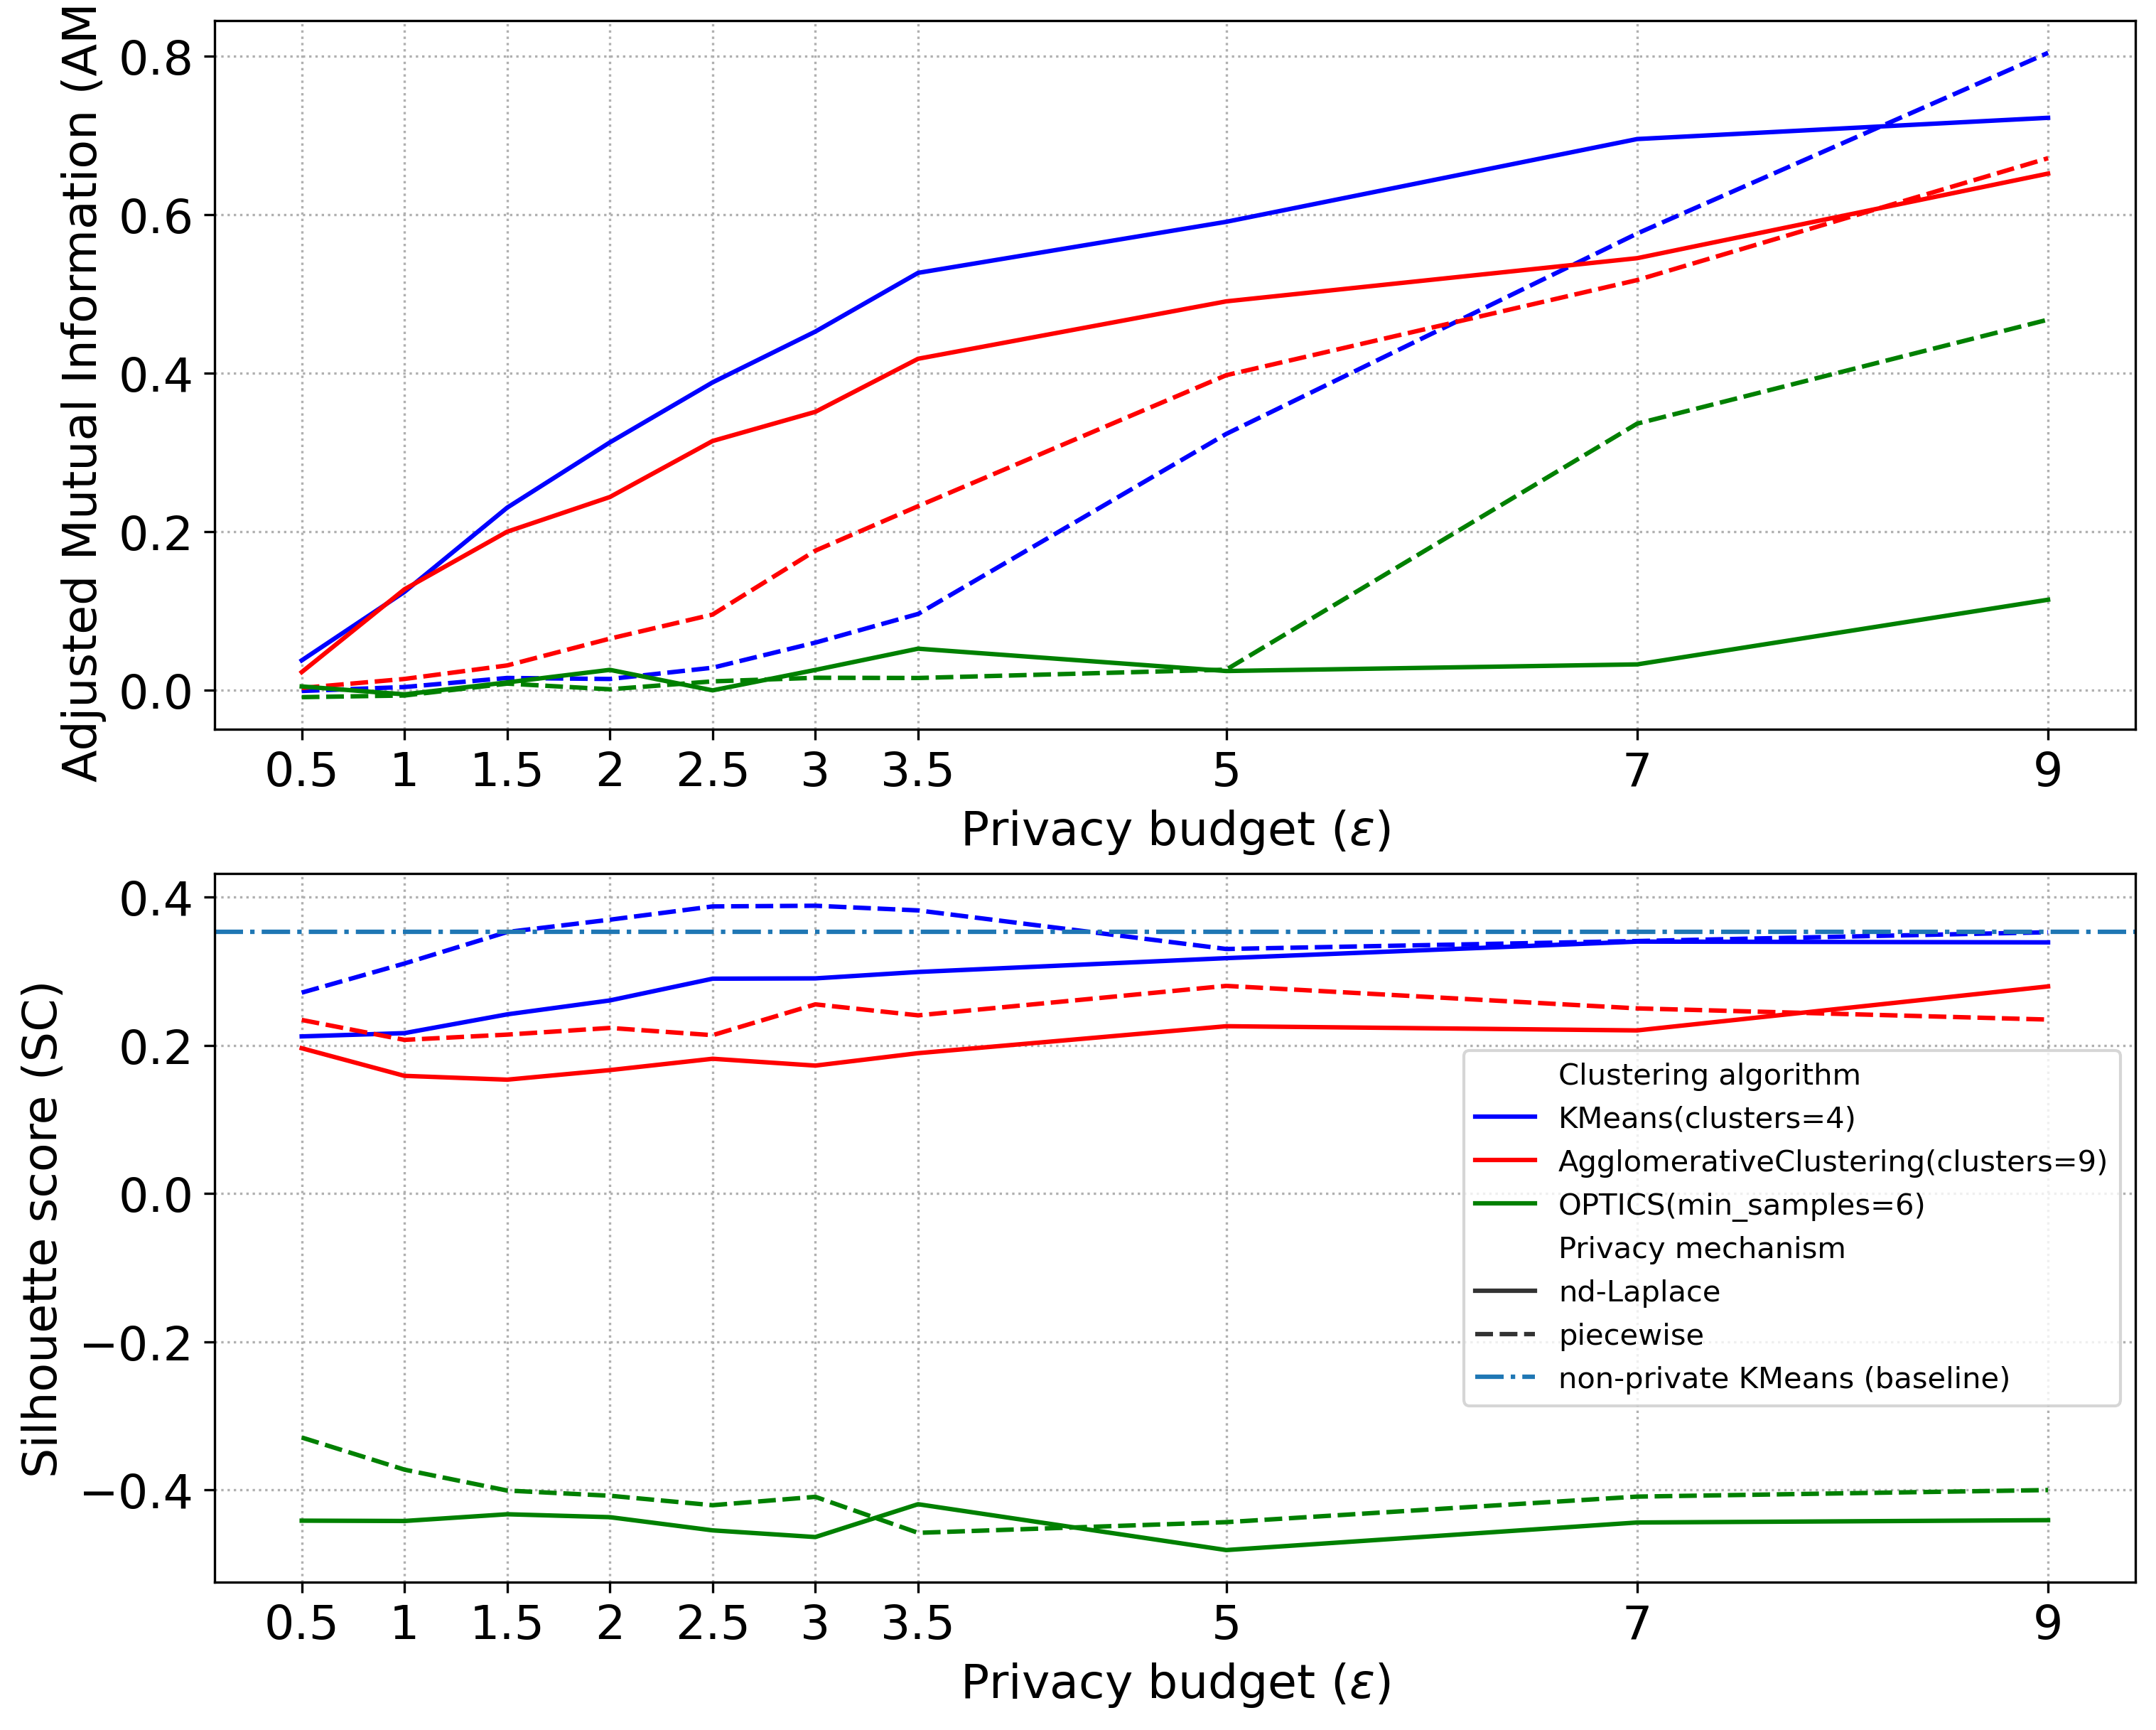
\includegraphics[width=0.9\textwidth]{Results/nd-laplace/nd-Laplace/skewed-dataset/ami-and-sc_3_dimensions.png}

  \label{fig:validation-skewed-dataset_comparison_3d-laplace}
\end{figure}
The nD-Laplace mechanism performs best with the K-Means algorithm, scoring approximately +/- 0.76 \gls{ami} for privacy budgets 7 and 9. \gls{ag} also scores well, reaching a maximum of 0.63 \gls{ami}. In contrast, \gls{optics} scores significantly lower.

For the Piecewise mechanism, we observe a similar pattern for K-Means and \gls{ag}. Although the progression of scores is alike, the actual scores only start to match from privacy budget 7 onwards. However, \gls{optics} scores much better from privacy budget 5.

For \gls{sc}, we see the same behavior, which we actually observe in every dataset. Both K-Means and \gls{ag} score close to the baseline value. In this case, \gls{ag} is slightly below K-Means.

From the results, it's evident that we see a similar trend in outcomes as with the heart-dataset. With nD-Laplace performing well at both lower and higher privacy budgets. When looking at the data distribution, it is spread out similarly to the heart-dataset. Whereas with the other datasets (especially circle/line), we noticed that the datasets have a strong shape.
\todo[inline]{Add some distribution image}.

\newpage
\subsection{n-dimensional data}
\begin{figure}[H]
  \centering

  \caption{\textbf{AMI (top) and SC (bottom) for the kD-Laplace and Piecewise mechanisms for the n-dimensional data seeds-dataset}}
  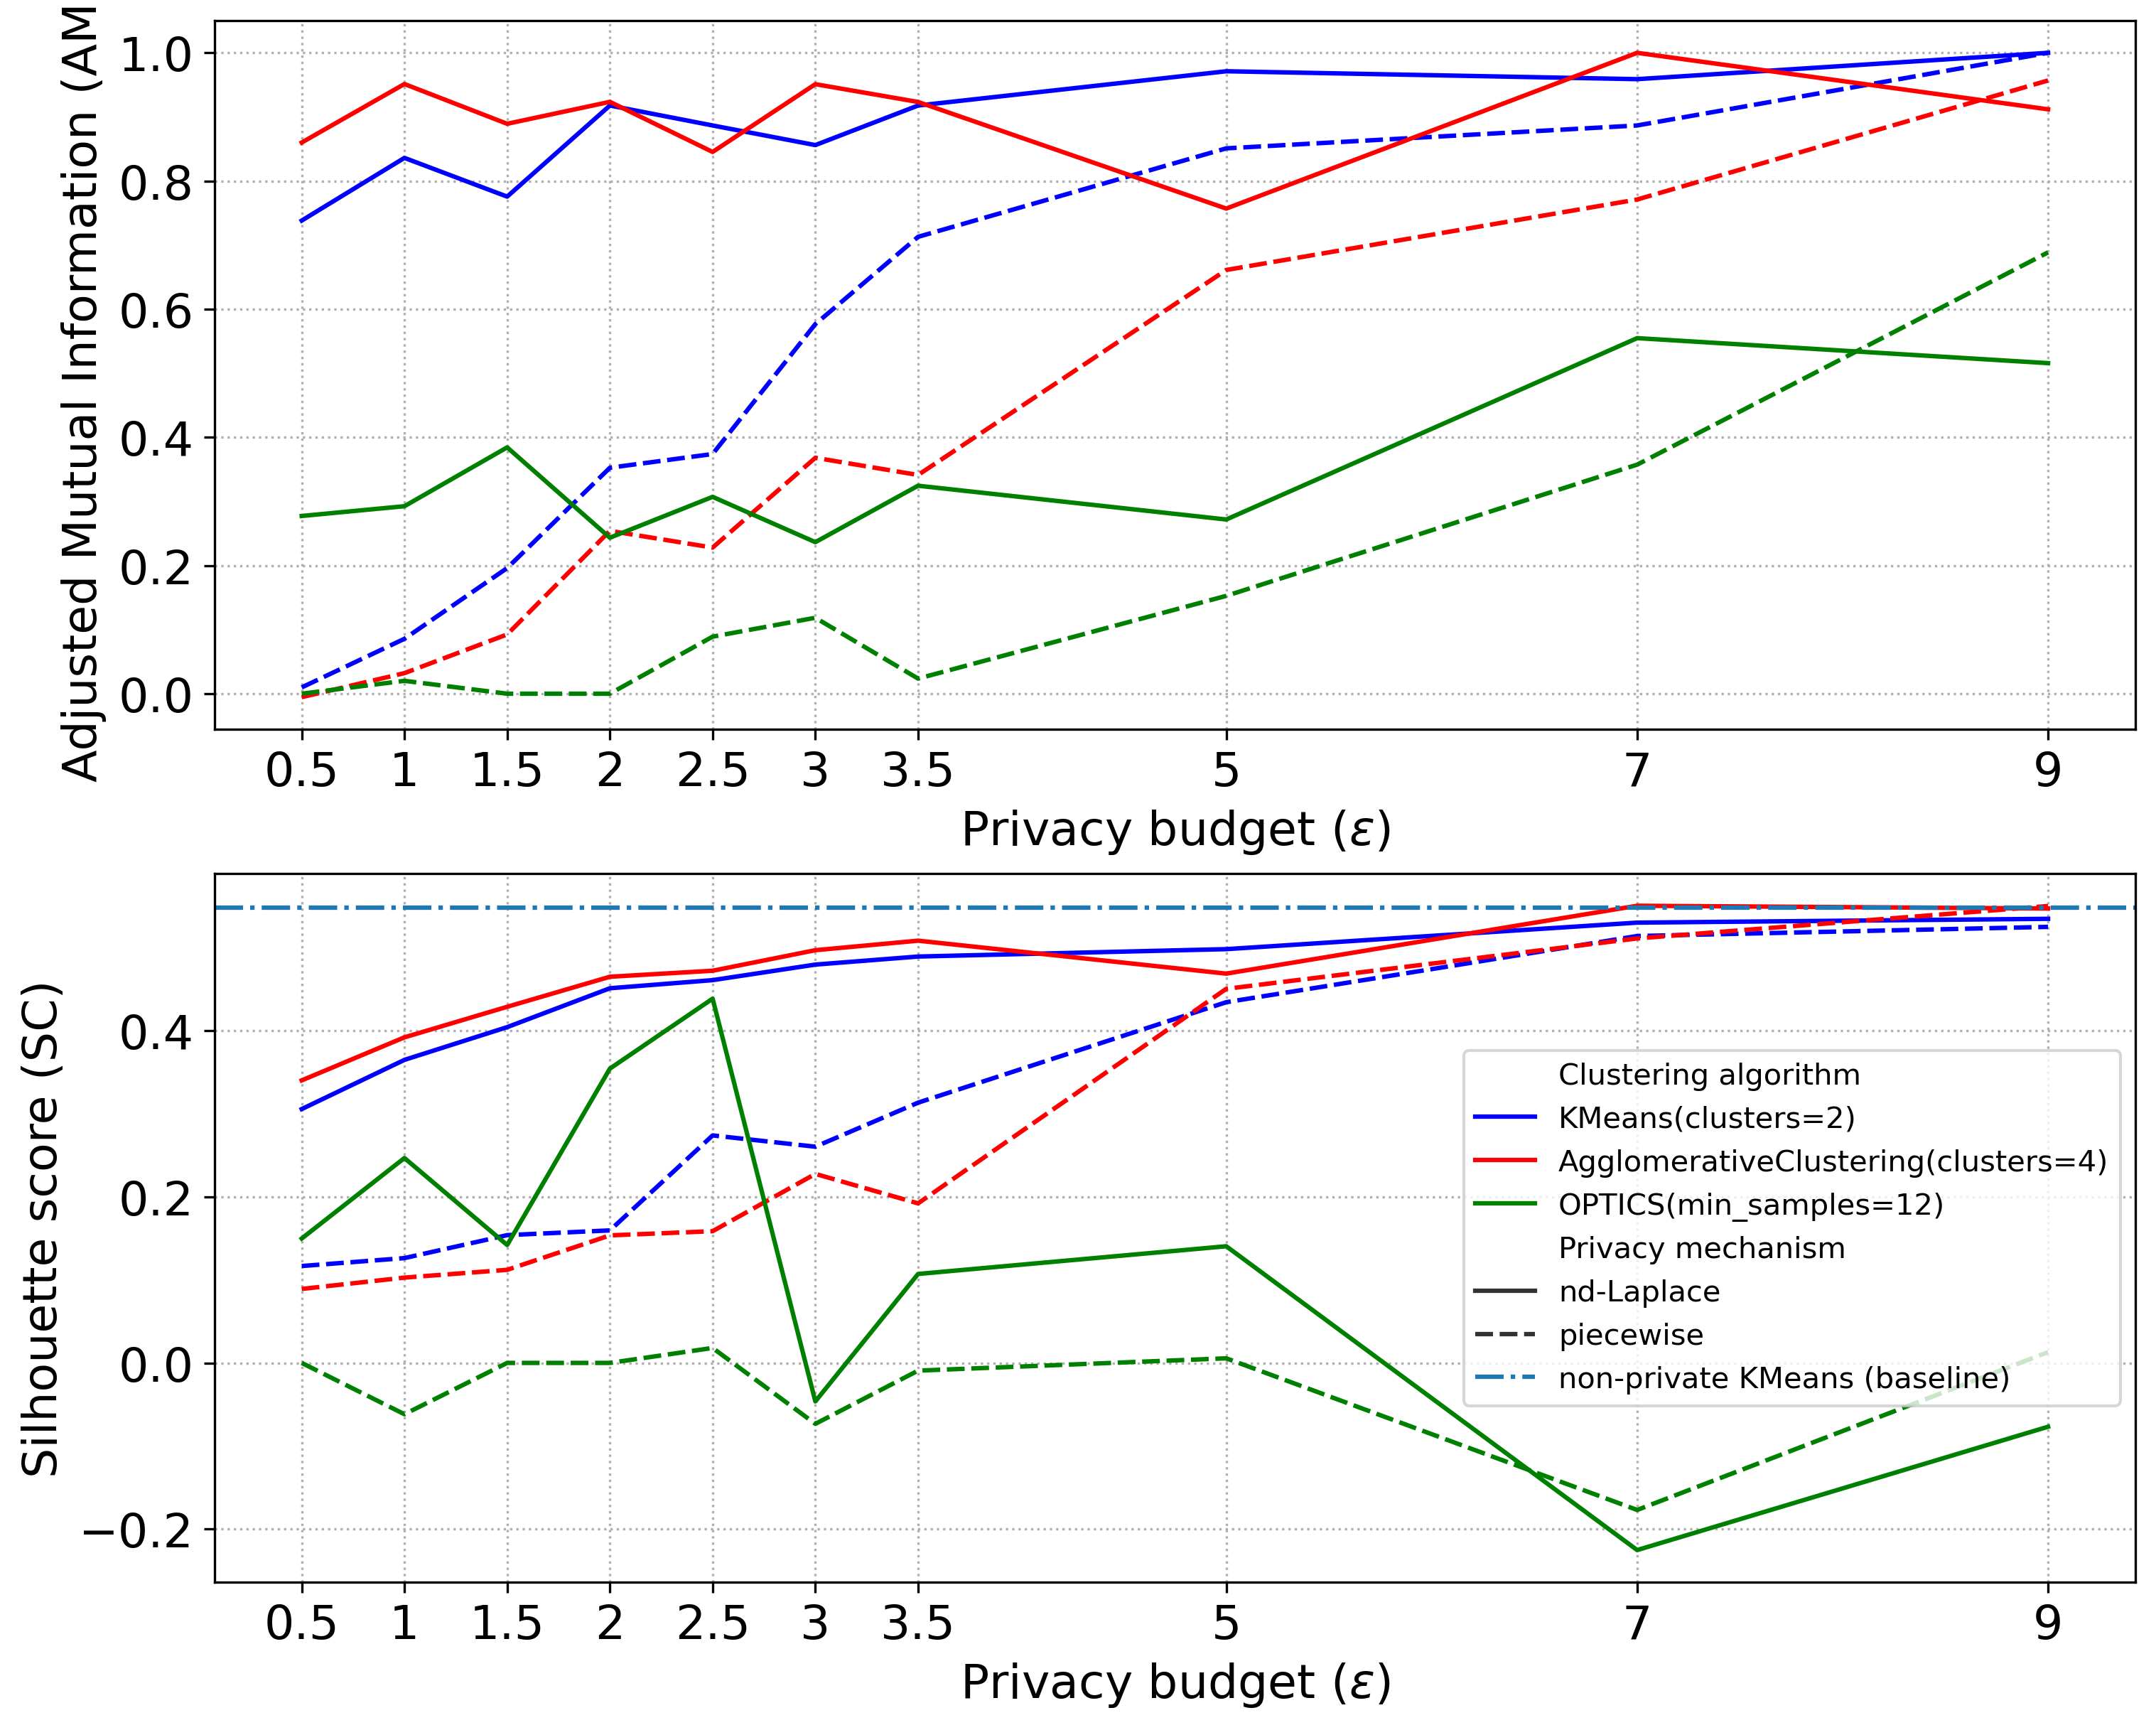
\includegraphics[width=0.9\textwidth]{Results/nd-laplace/nd-Laplace/seeds-dataset/ami-and-sc_7_dimensions.png}

  \label{fig:validation-seeds-dataset_comparison_nd-laplace}
\end{figure}
For n-dimensional data, we observe that nD-Laplace consistently scores high from privacy budget 0.5 up to 9. This applies to both K-Means and \gls{ag}. \gls{optics} also shows some improvements, scoring between 0.25 and 0.55 from epsilon 0.5 to 9.

The Piecewise mechanism only starts to show comparable results from a privacy budget of 5. From that point on, the results for K-Means and \gls{ag} are almost identical. For \gls{optics}, Piecewise scores slightly higher at a privacy budget of 9, but for the other privacy budgets, nD-Laplace performs better.

For \gls{sc}, we see a bit more variation between the mechanisms than with the other dimensions. Also, The trend of \gls{sc} seems more similar to that of \gls{ami} than what we've observed in other dimensions. 
Looking at the scores, the nD-Laplace mechanism scores below the baseline from privacy budgets 0.5 to 7 but matches the scores for K-Means and \gls{ag} afterward. For nD-Laplace, \gls{optics} starts at 0.2 \gls{sc}, but then drops below 0. The Piecewise mechanism remains below 0 for \gls{optics} across all privacy budgets.

Something notable occurs for the privacy budget of 2.5, as \gls{optics} peaks at 2.5. We would only expect this at a privacy budget of 9 when less noise has been added.
\todo[inline]{We have to research this.}
\newpage
\begin{figure}[H]
  \centering

  \caption{\textbf{AMI (top) and SC (bottom) for the kD-Laplace and Piecewise mechanisms for the n-dimensional data heart-dataset}}
  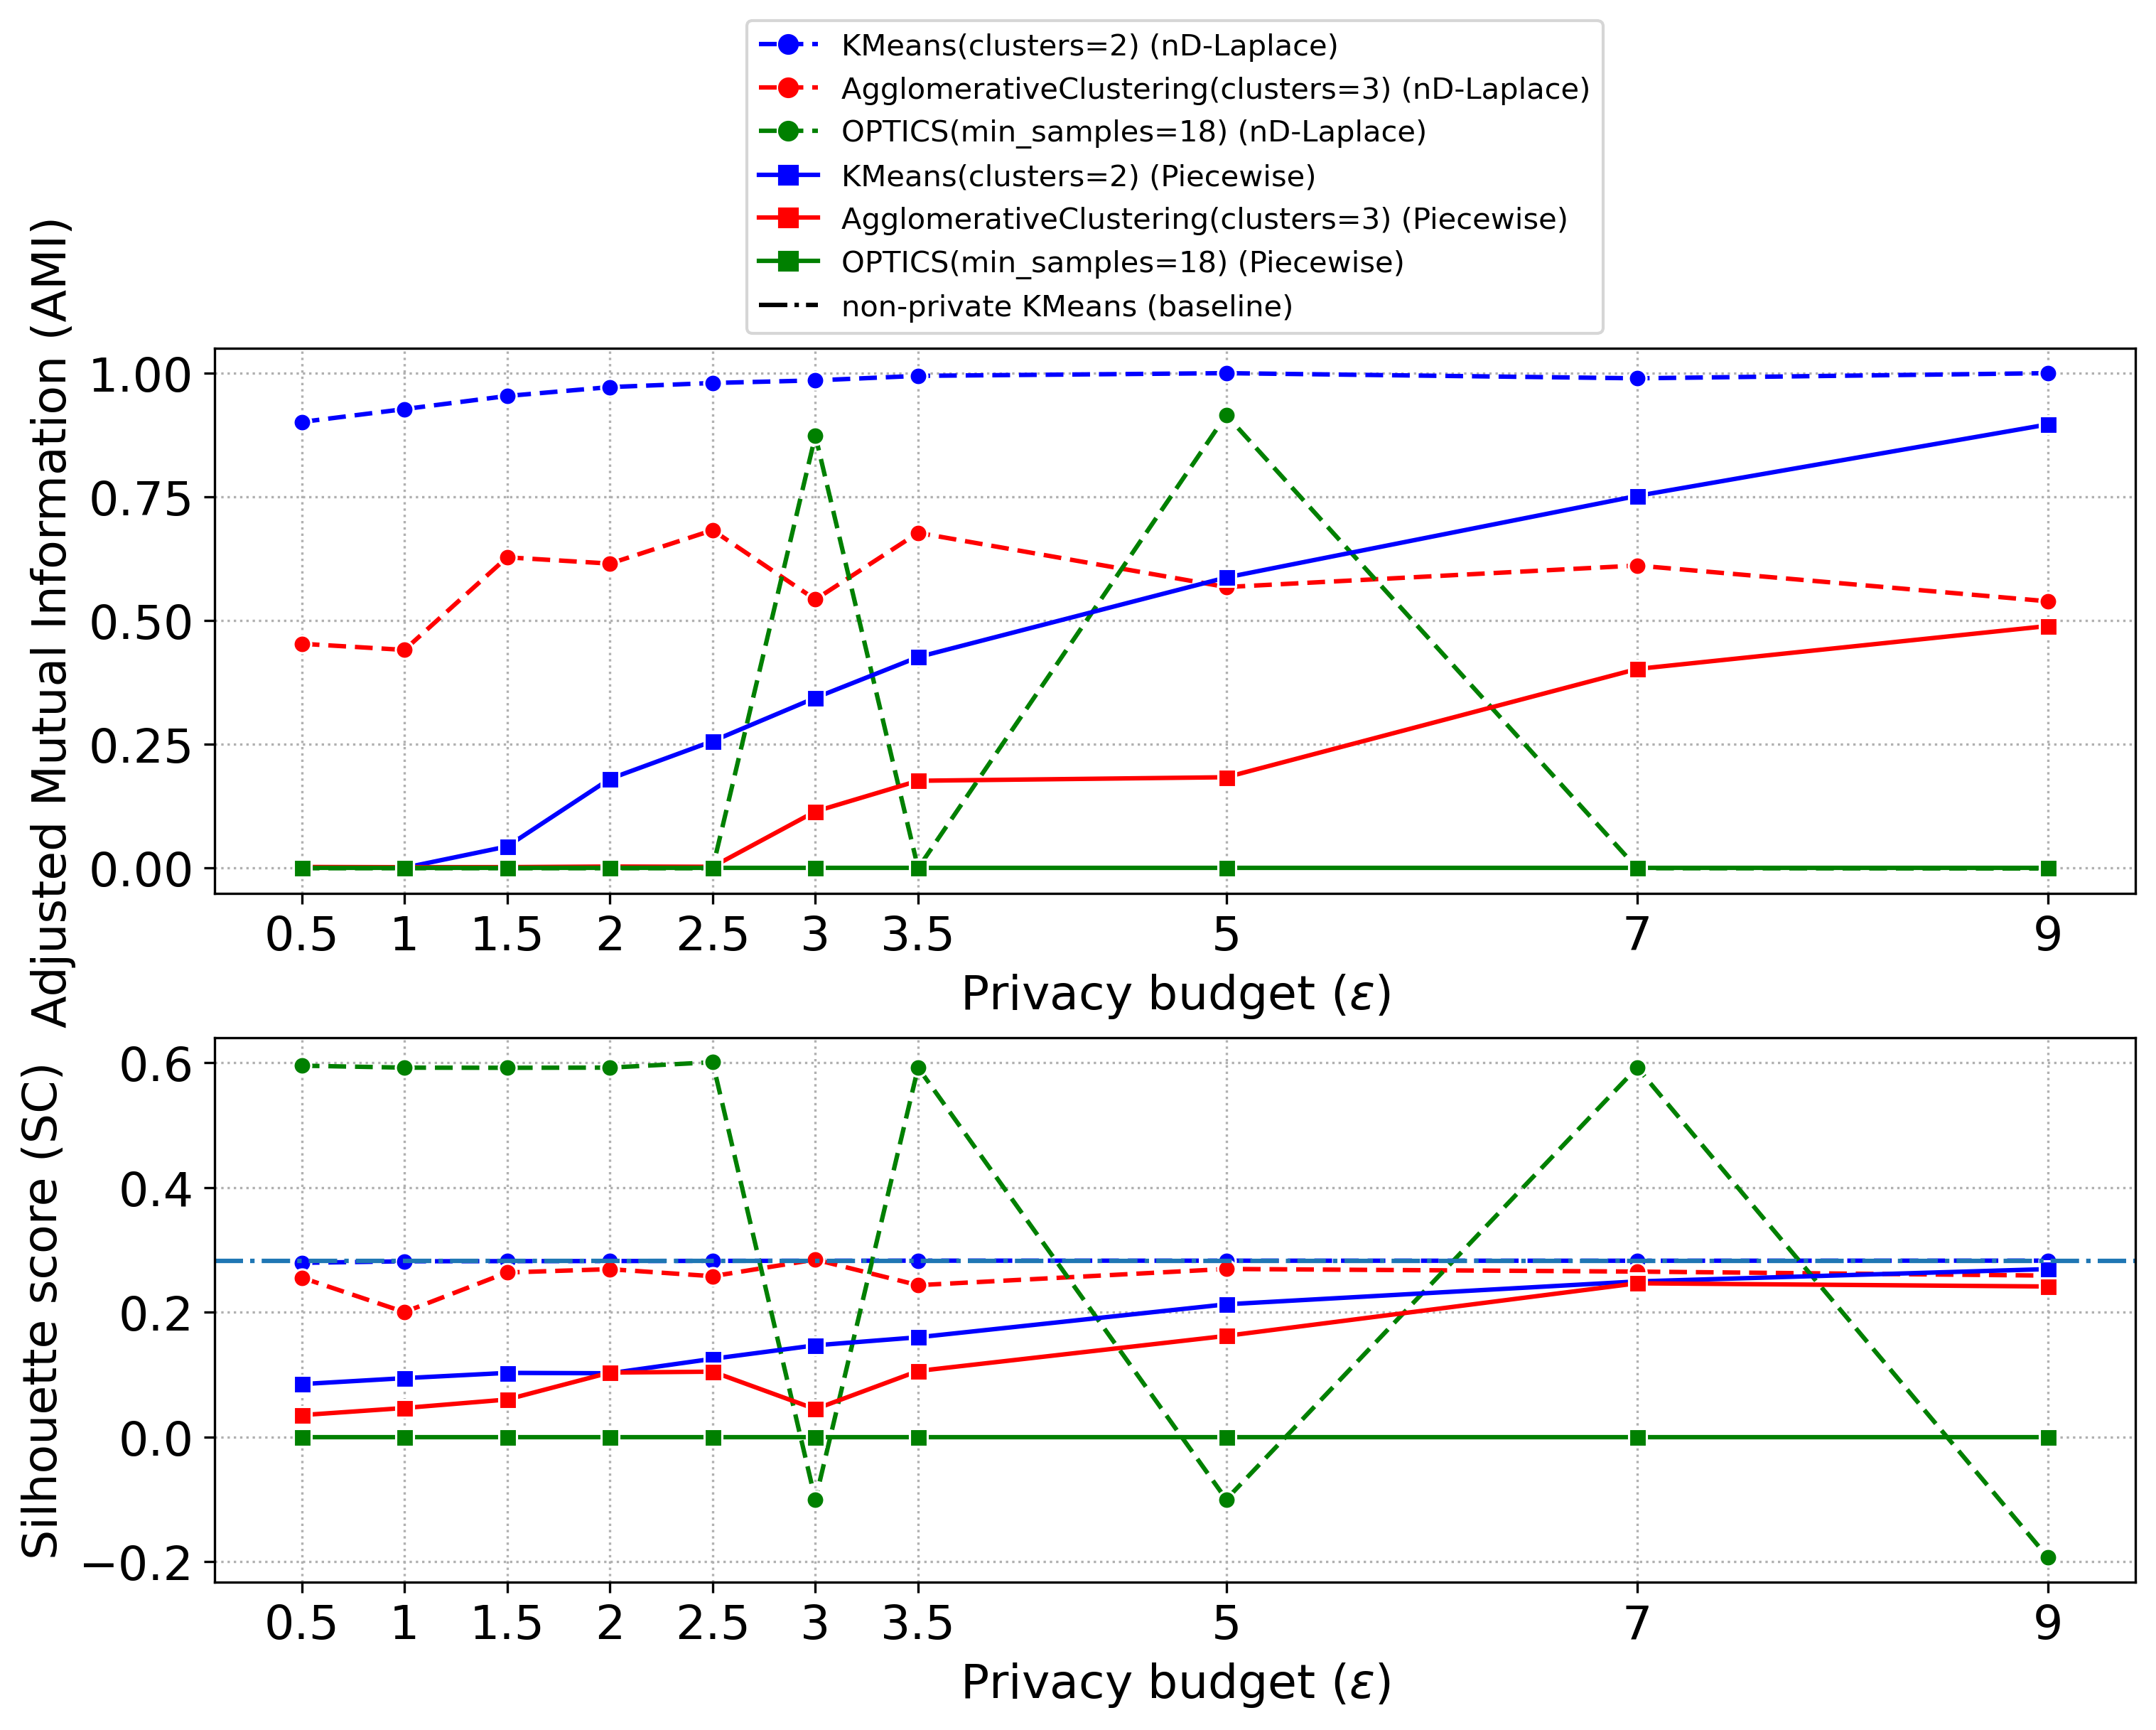
\includegraphics[width=0.9\textwidth]{Results/nd-laplace/nd-Laplace/heart-dataset/ami-and-sc_9_dimensions.png}

  \label{fig:validation-heart-dataset_comparison_nd-laplace}
\end{figure}
For nD-Laplace, the heart-dataset consistently scores very well for K-Means. Even for n-dimensional data, the result consistently remains above 0.95 \gls{ami} for all privacy budgets.
For \gls{ag}, a good score is achieved, but it plateaus around 0.6 \gls{ami}.
With \gls{optics}, the data is quite inconsistent, ranging from 0 to 0.90 \gls{ami}.
The Piecewise mechanism shows a similar trend for both K-Means and \gls{ag}, with K-Means performing the best. Both score below nD-Laplace across all privacy budgets.
For \gls{optics}, the score remains at 0 for the Piecewise mechanism.
With the \gls{sc} metric, the same pattern is evident, but the \gls{sc} is relatively low when considering the high \gls{ami} achieved. For \gls{optics}, an odd result is observed, as it scores 0.6 \gls{ami} (0.25 above the baseline) from 0.5 to 3. However, for privacy budgets of 3, 5, and 9, the score drops back to 0 \gls{sc}.

\todo[inline]{Analyse gedrag}

\newpage
\section{Mechanism utility}
The sections below present a heatmap comparison of the nd-Laplace and Piecewise mechanisms.
We employed a heatmap to simultaneously depict the privacy budget (epsilon), the number of dimensions, and a specific metric. The metric in focus is the \gls{ami}, which is determined using the K-Means algorithm.
We opted for K-Means as it consistently delivered reliable results across all our experiments, making it an ideal baseline for gauging the \gls{ami}.

On the heatmap, the x-axis represents the privacy budget, while the y-axis illustrates the number of dimensions. Each cell of the heatmap conveys the \gls{ami} value. The intensity of the cell's color corresponds to the \gls{ami} score: a darker shade signifies a higher score. Consequently, the darker (or higher) the score, the more favorable the outcome. \newline

The results for the shape datasets (Circle, Line and Skewed) were omitted, because we do not have more then 3 dimensions. Therefore, the heat maps do not yield a lot of information in addition to the cluster utility plots.

Please refer to the plots in the appendix for:
\begin{enumerate}
  \item Privacy distance: \ref{appendix:results-privacy}.
  \item True Positive Rate: \ref{appendix:results-privacy}.
\end{enumerate}
\newpage
\subsection{Seeds-dataset}
\begin{figure}[H]
  \centering
  \begin{subfigure}[b]{0.8\textwidth}
    \begin{subfigure}[c]{1\textwidth}
      \caption{\textbf{Adjusted Mutual Information comparison for the kd-Laplace mechanism}}
      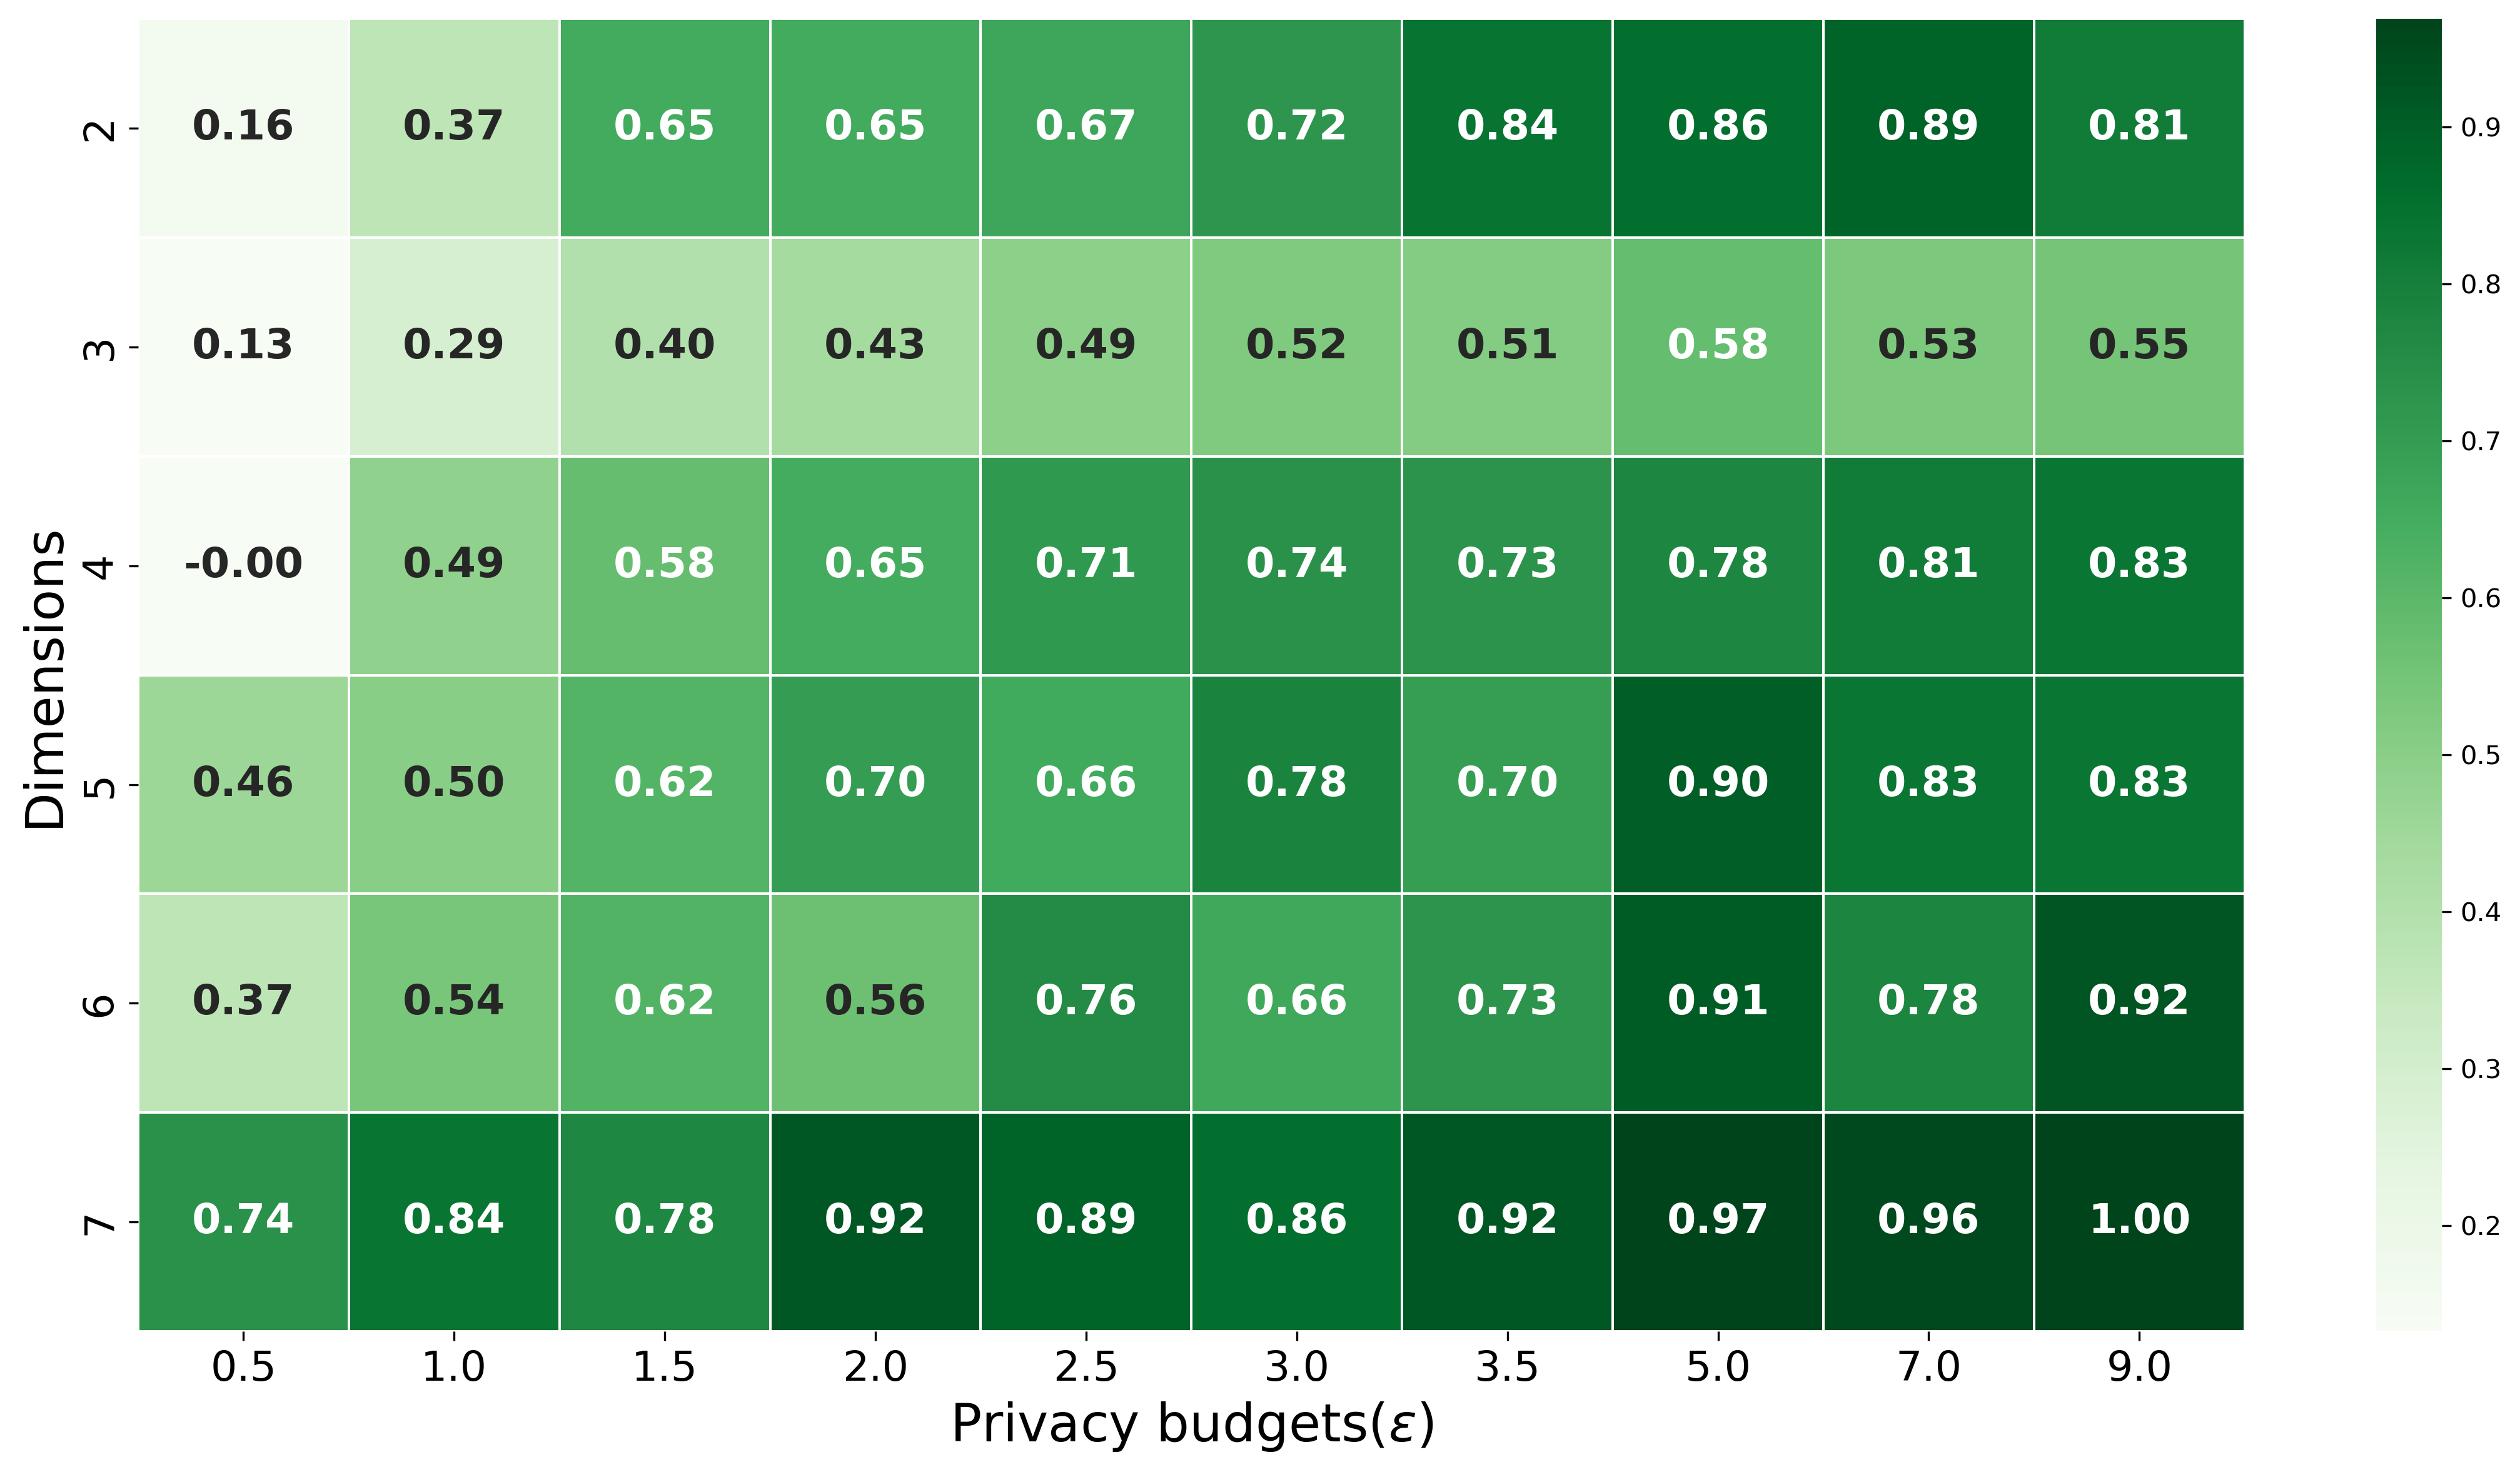
\includegraphics[width=1\textwidth]{Results/nd-laplace/nd-Laplace/seeds-dataset/ami.png}
      \label{fig:ami_seeds-dataset_comparison_kdlaplace_2d}
    \end{subfigure}
    \vfill % vertical space
    \begin{subfigure}[c]{1\textwidth}
      \caption{\textbf{Adjusted Mutual Information comparison for the Piecewise mechanism}}
      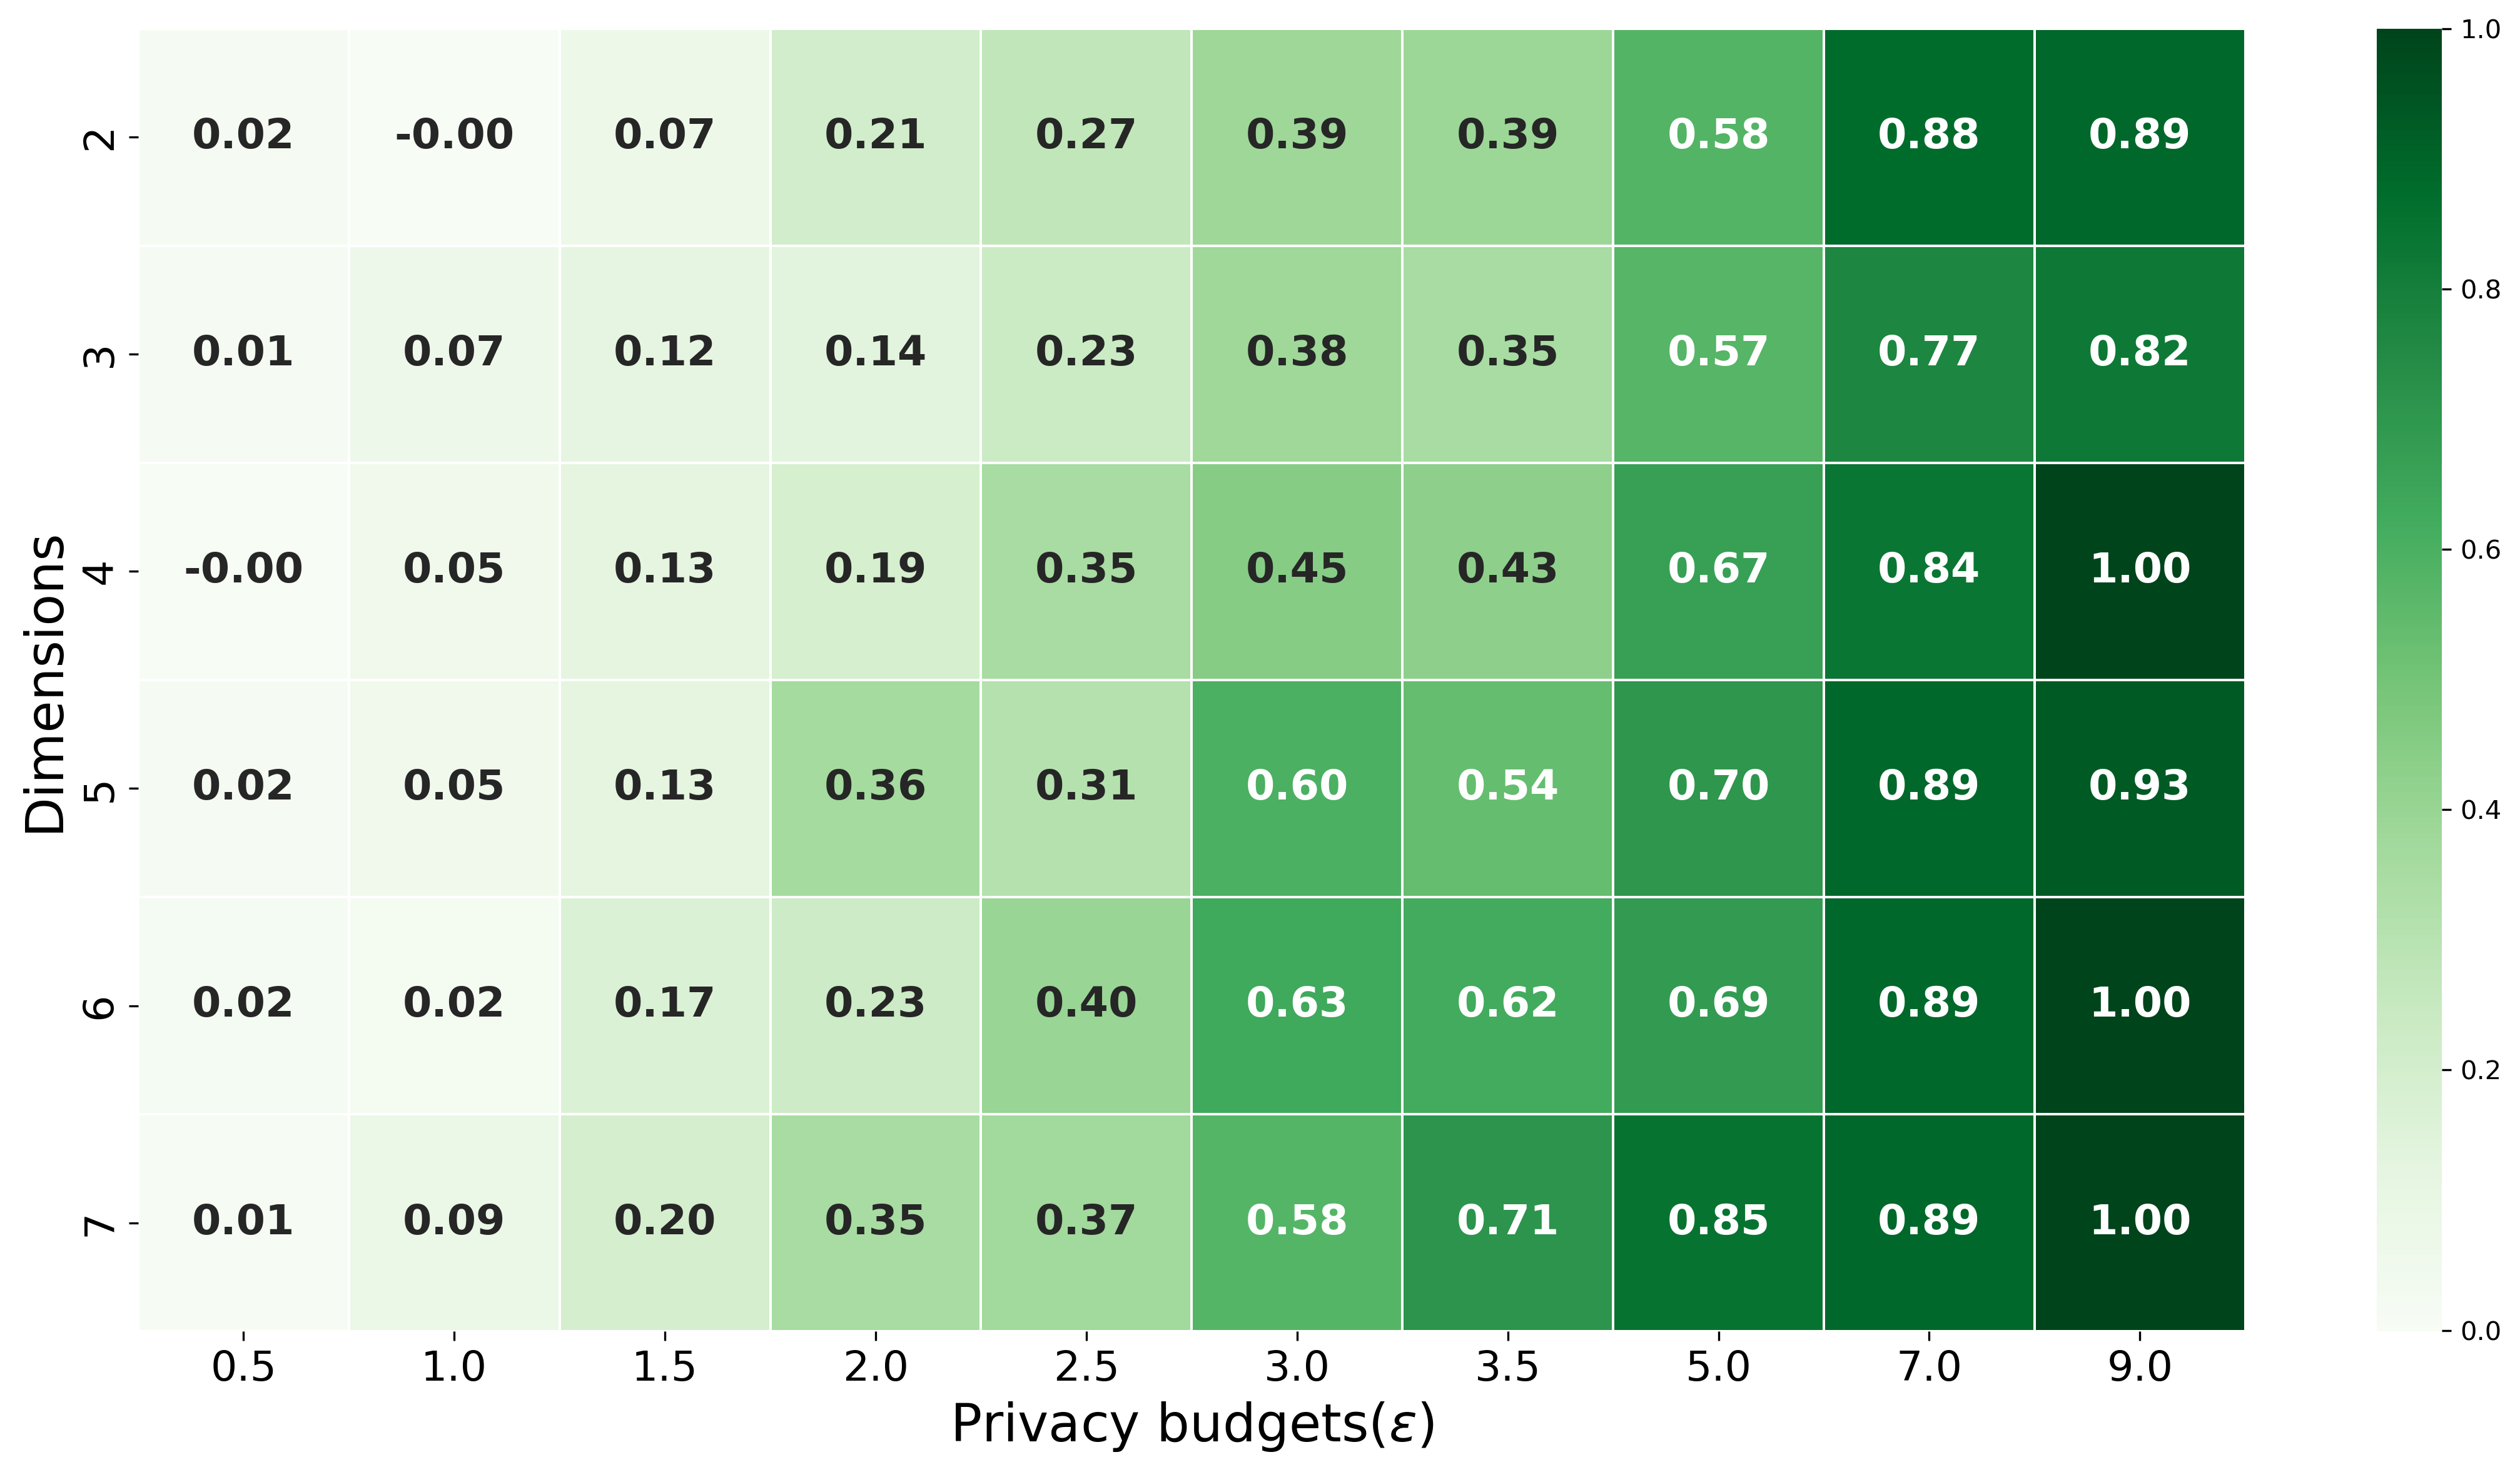
\includegraphics[width=1\textwidth]{Results/nd-laplace/piecewise/seeds-dataset/ami.png}
      \label{fig:ami_seeds-dataset_comparison_piecewise_2d}
    \end{subfigure}
  \end{subfigure}
  
\end{figure}
For the heatmaps, we observe a similar pattern, which was also evident in the cluster analysis. Specifically, nD-Laplace consistently scores well from lower epsilons, while Piecewise only starts to perform well from a privacy budget of 3.
For nD-Laplace, the number of dimensions influences the score. The implementation of 3D-Laplace, in particular, scores relatively low. From 4 dimensions onward, we notice an increase in the \gls{ami}, especially in combination with an increasing \gls{epsilon}.
For Piecewise, it's notable that the number of dimensions has minimal impact on the outcome, with the privacy budget being the primary influencing factor. However, dimension does play a role for privacy budgets between 3 and 5, as scores are higher from 5 dimensions compared to lower dimensions.

For nD-Laplace, the dimensions can significantly influence the improved result because as the number of dimensions increases, the noise decreases. We've elaborated on this phenomenon in Section \ref{fig:curse-of-dimensionality}. As a result, more information is retained, leading to an increase in score with the number of dimensions. The Piecewise mechanism might also be affected by this, but to a lesser extent.
\todo[inline]{Further research needed}

\newpage
\subsection{Heart-dataset}
\begin{figure}[H]
  \centering
  \begin{subfigure}[b]{0.80\textwidth}
    \begin{subfigure}[c]{1\textwidth}
      \caption{\textbf{Adjusted Mutual Information comparison for the kd-Laplace mechanism}}
      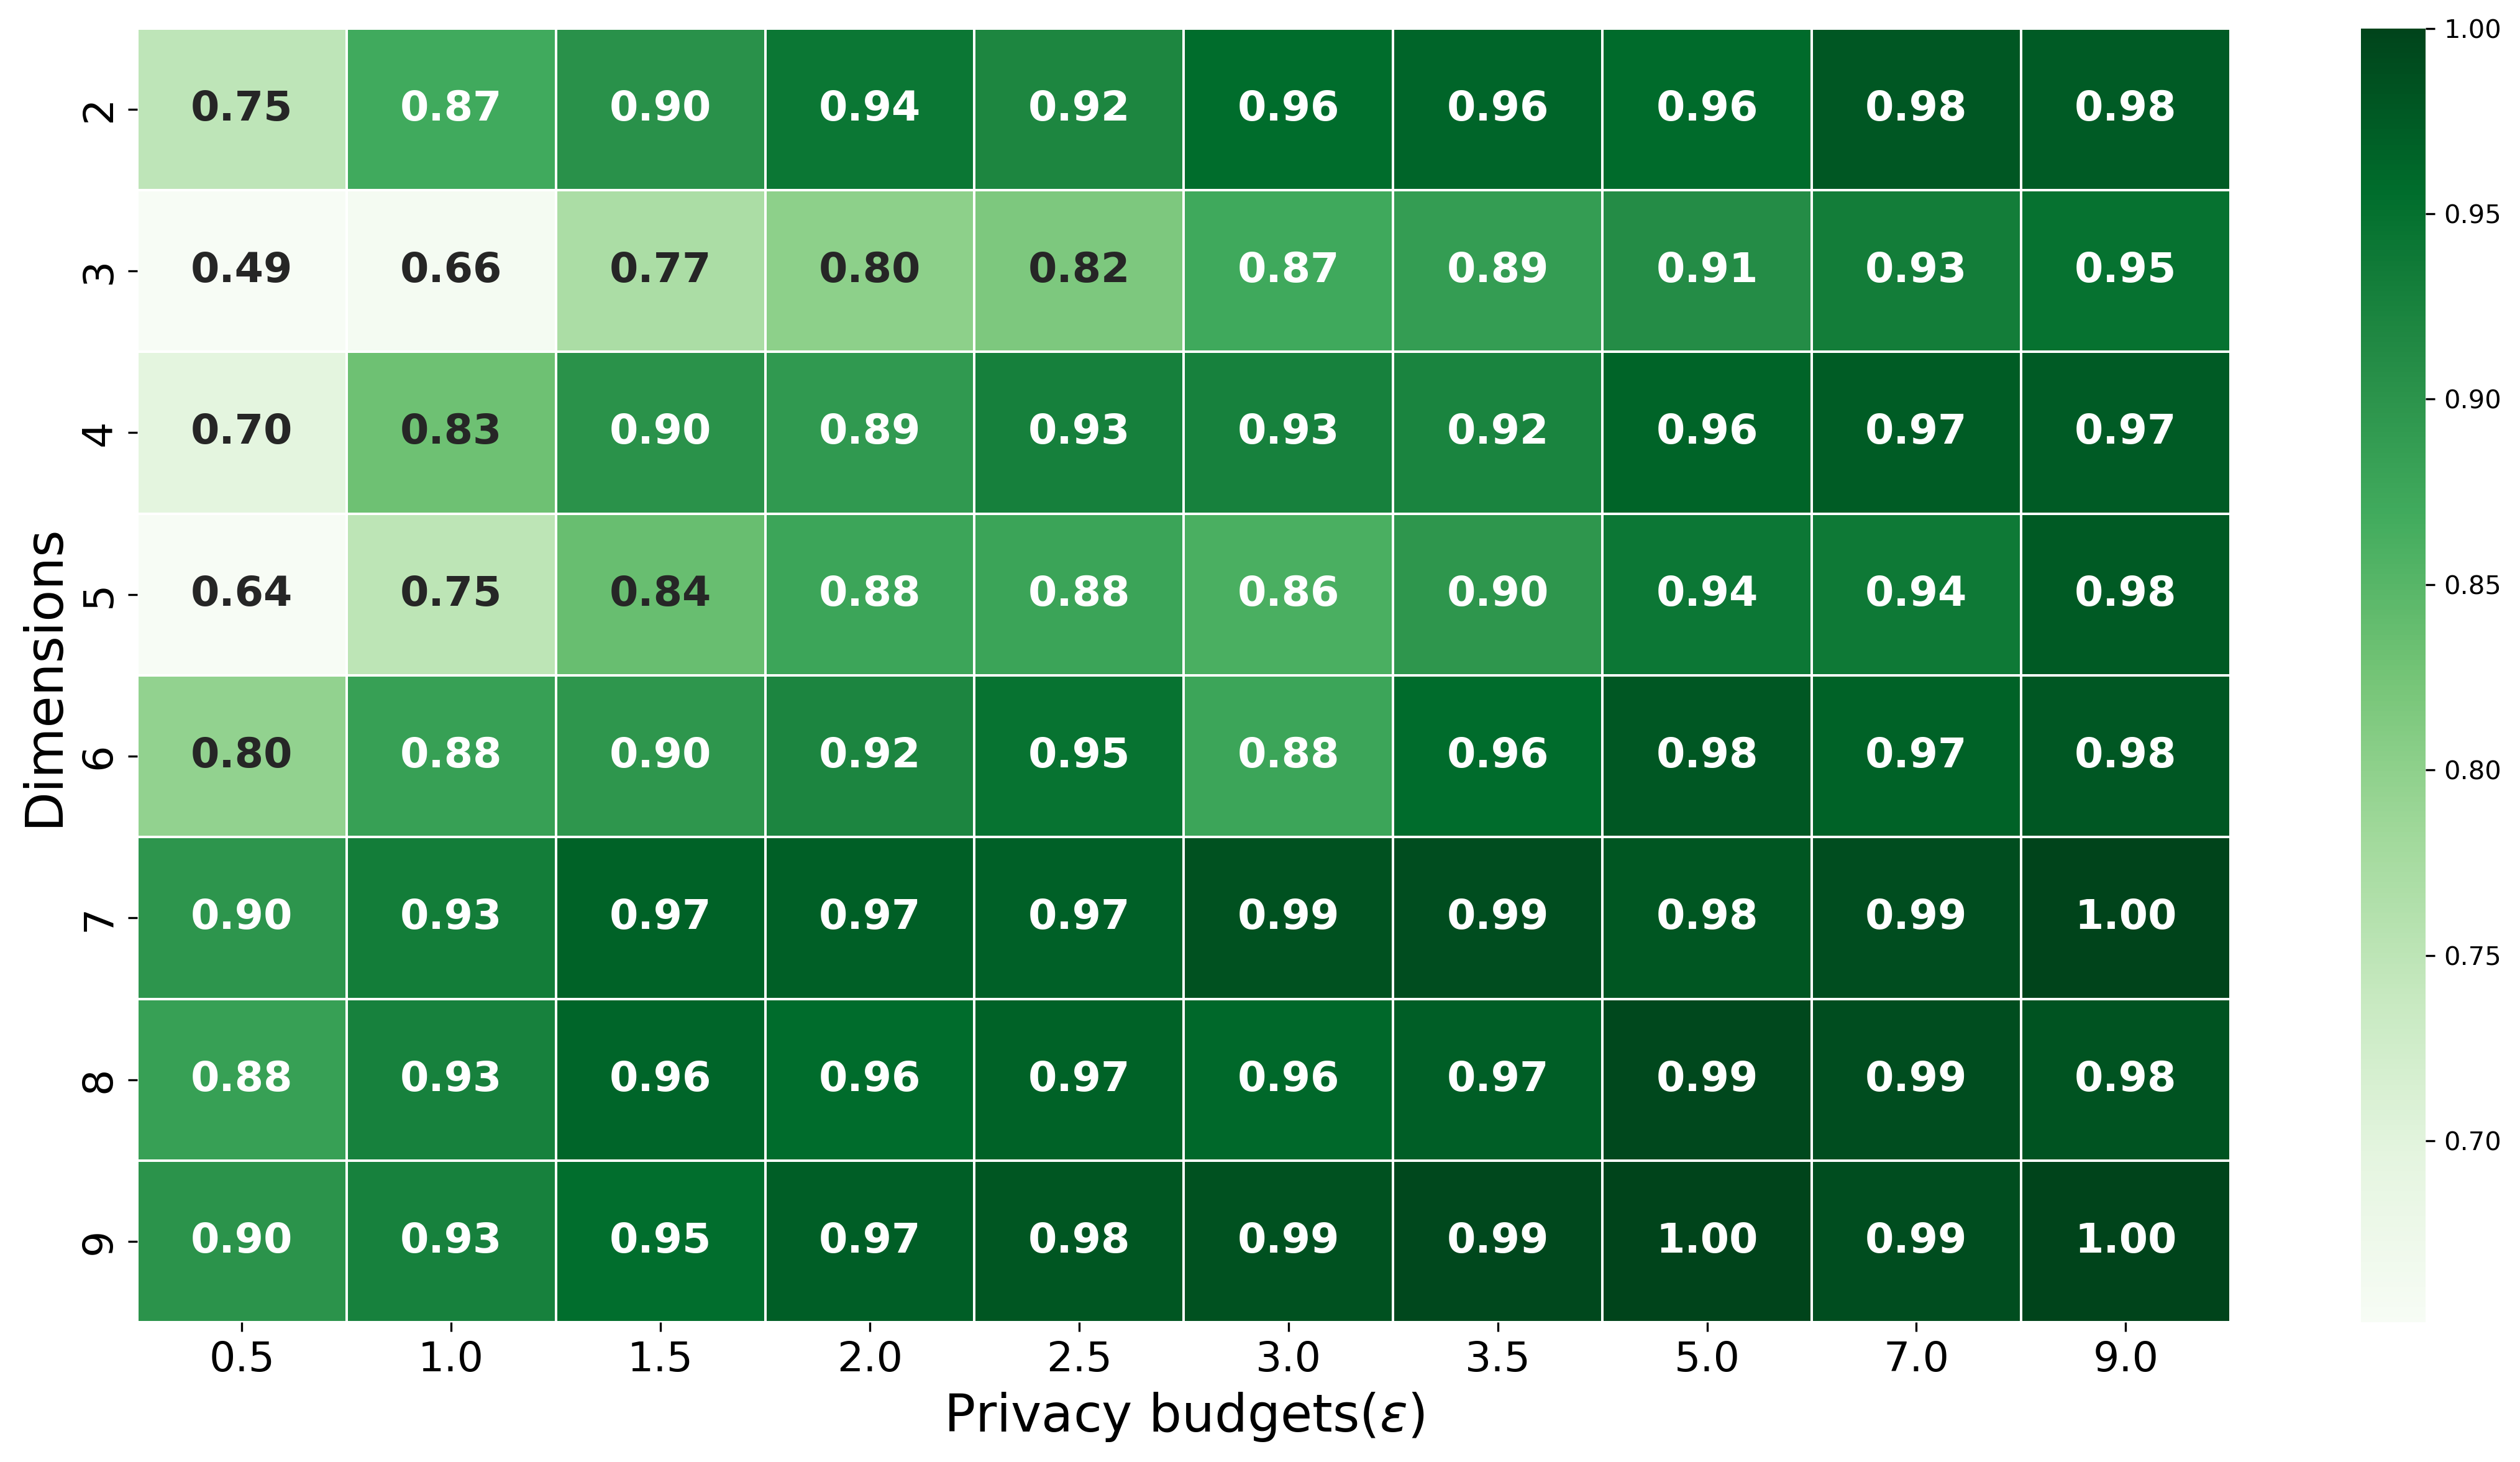
\includegraphics[width=1\textwidth]{Results/nd-laplace/nd-Laplace/heart-dataset/ami.png}
      \label{fig:ami_heart-dataset_comparison_kdlaplace_2d}
    \end{subfigure}
    \vfill % vertical space
    \begin{subfigure}[c]{1\textwidth}
      \caption{\textbf{Adjusted Mutual Information comparison for the Piecewise mechanism}}
      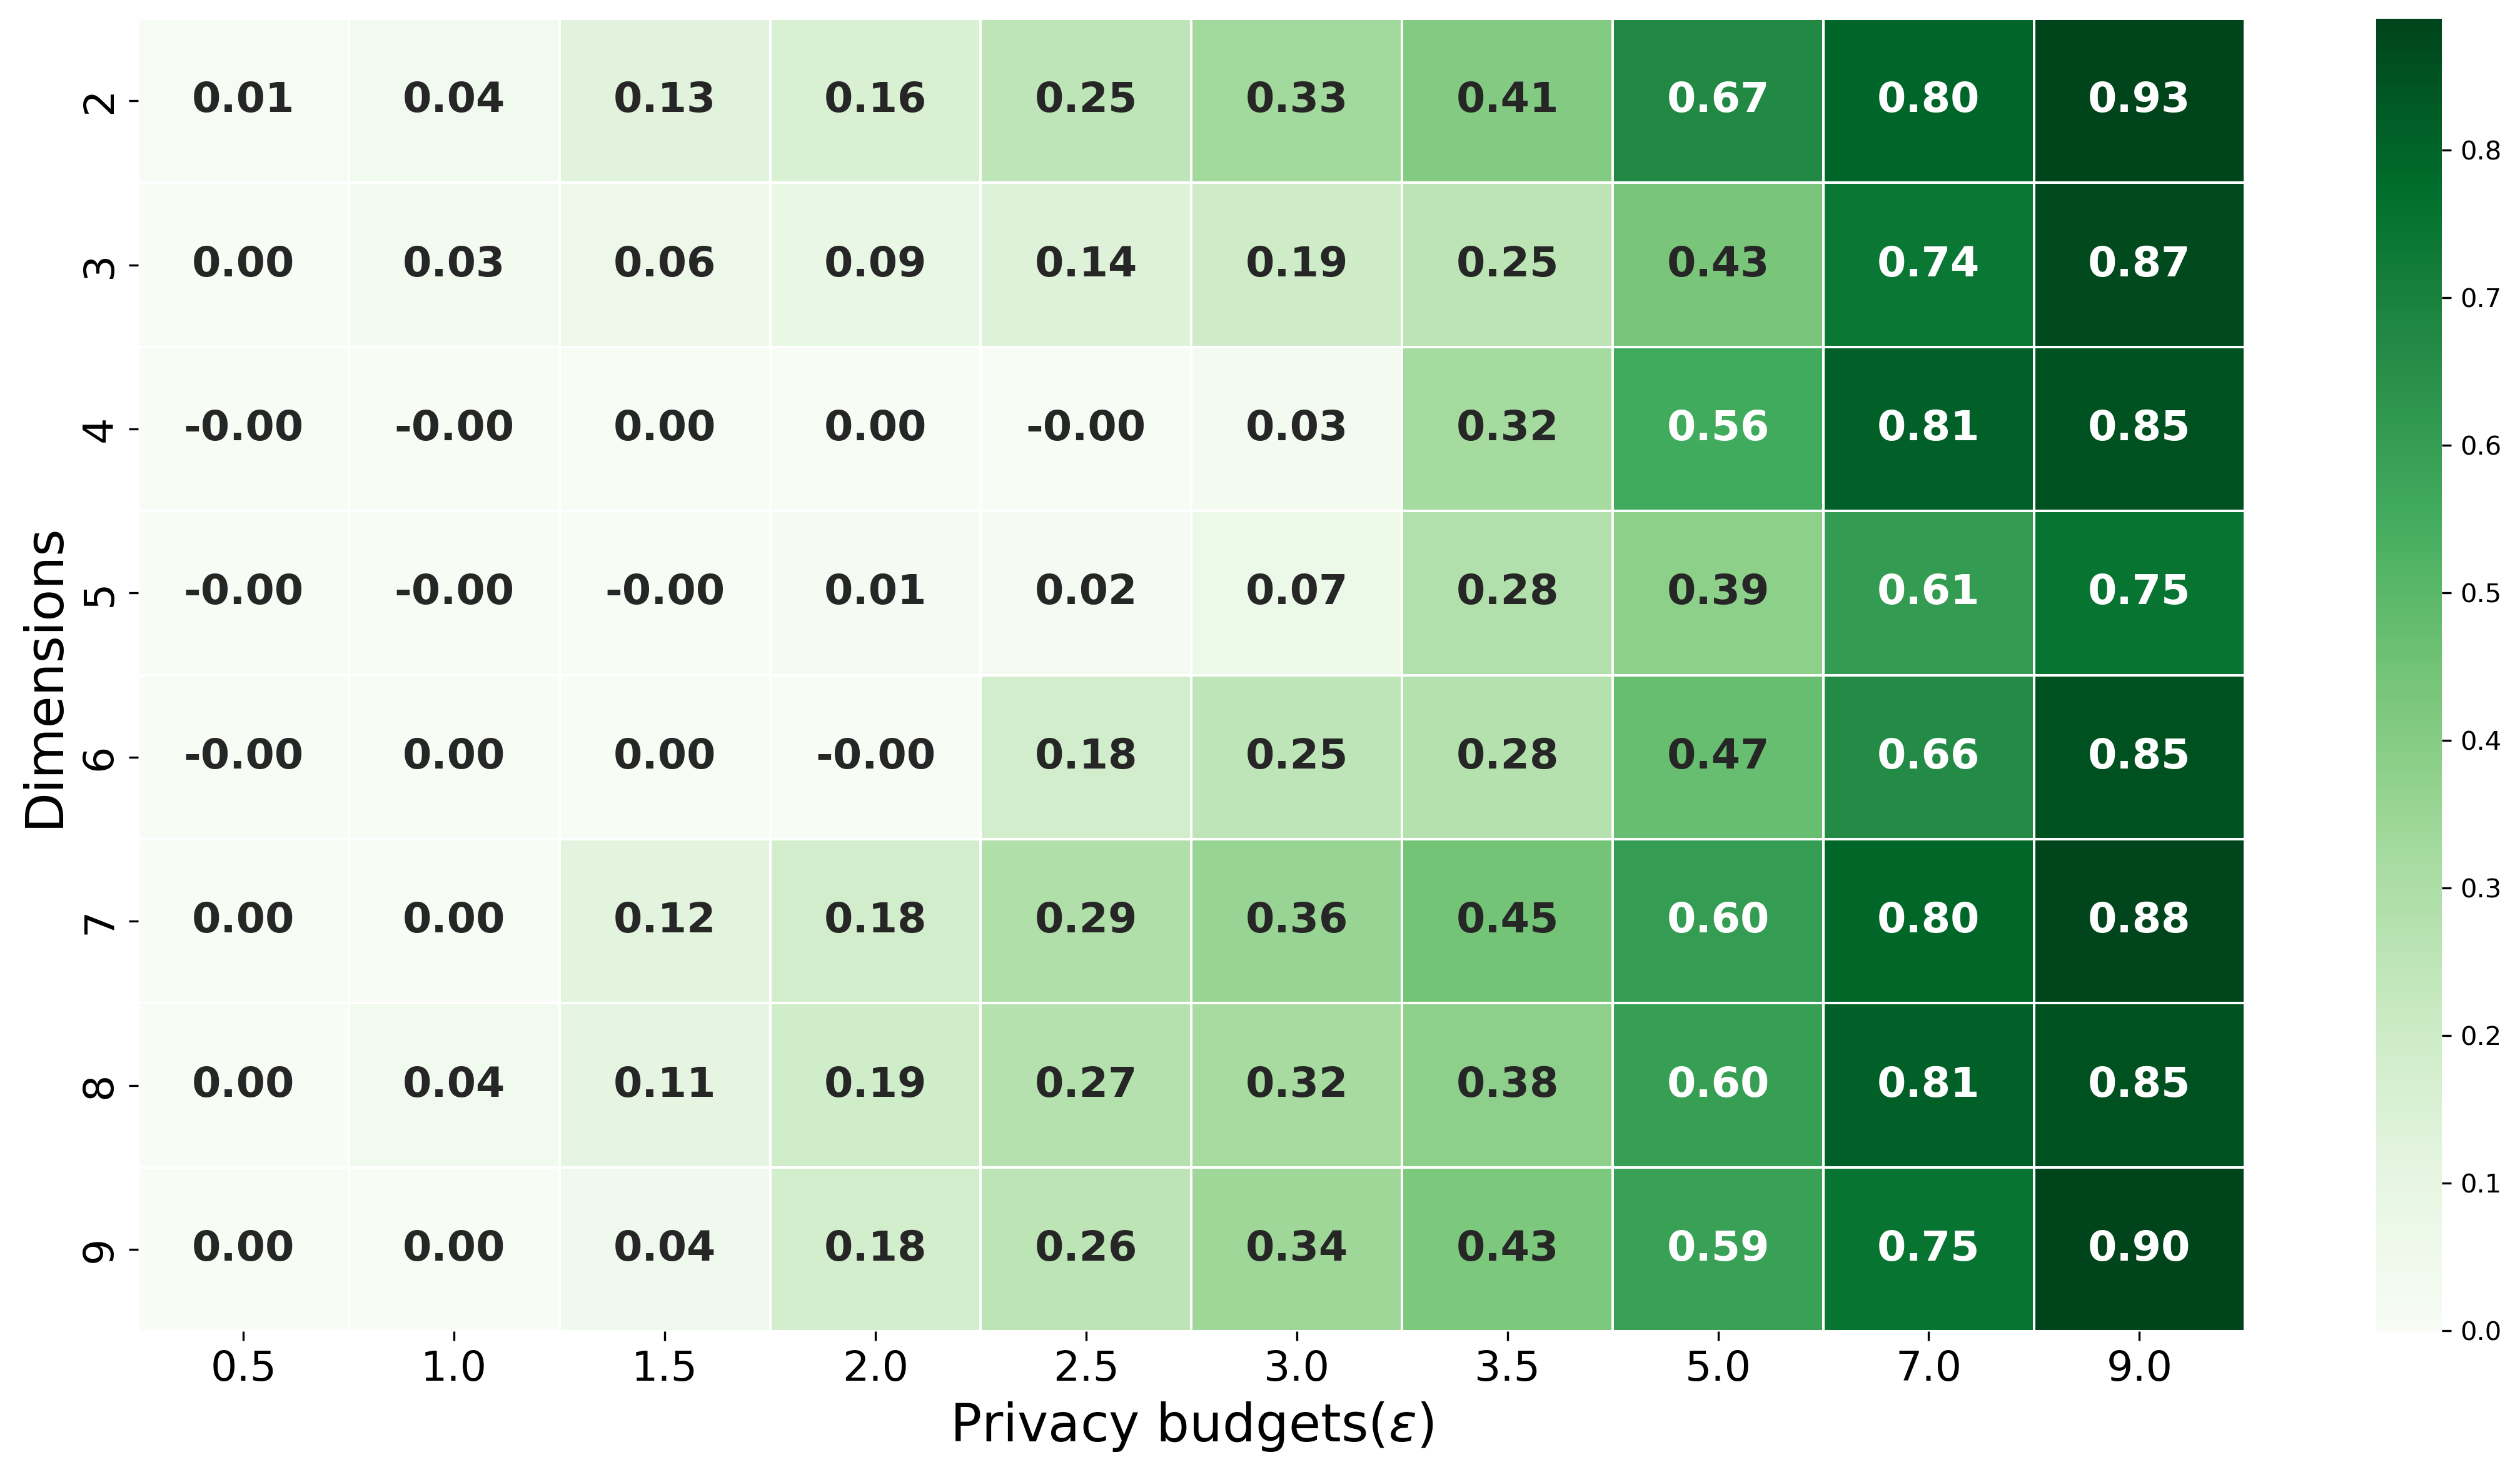
\includegraphics[width=1\textwidth]{Results/nd-laplace/piecewise/heart-dataset/ami.png}
      \label{fig:ami_heart-dataset_comparison_piecewise_2d}
    \end{subfigure}
  \end{subfigure}
\end{figure}
The scores for the heart-dataset are, as expected, in favor of nD-Laplace. We observe the same trend as in the cluster analysis, where nD-Laplace performs well across almost all privacy budgets. The performance of the 3D-Laplace implementation is slightly inferior, a finding that was also noted for the seeds-dataset. The influence of dimensions appears to be somewhat less pronounced than in the seeds-dataset, but from the 5th dimension onward, its impact becomes more significant.

The Piecewise mechanism scores low for privacy budgets between 0.5 and 3. Notably, the scores for 4 and 5 dimensions are considerably lower for these privacy budgets. Beyond that, the number of dimensions has minimal influence on the outcomes, with the privacy budget being the primary determinant.
\todo[inline]{Why are the 4 / 5 dimensions worse?}
\newpage
\mycomment{
\subsection{Circle-dataset}
\begin{figure}[H]
  \centering
  \begin{subfigure}[b]{0.8\textwidth}
    \begin{subfigure}[c]{1\textwidth}
      \caption{\textbf{Adjusted Mutual Information comparison for the kd-Laplace mechanism}}
      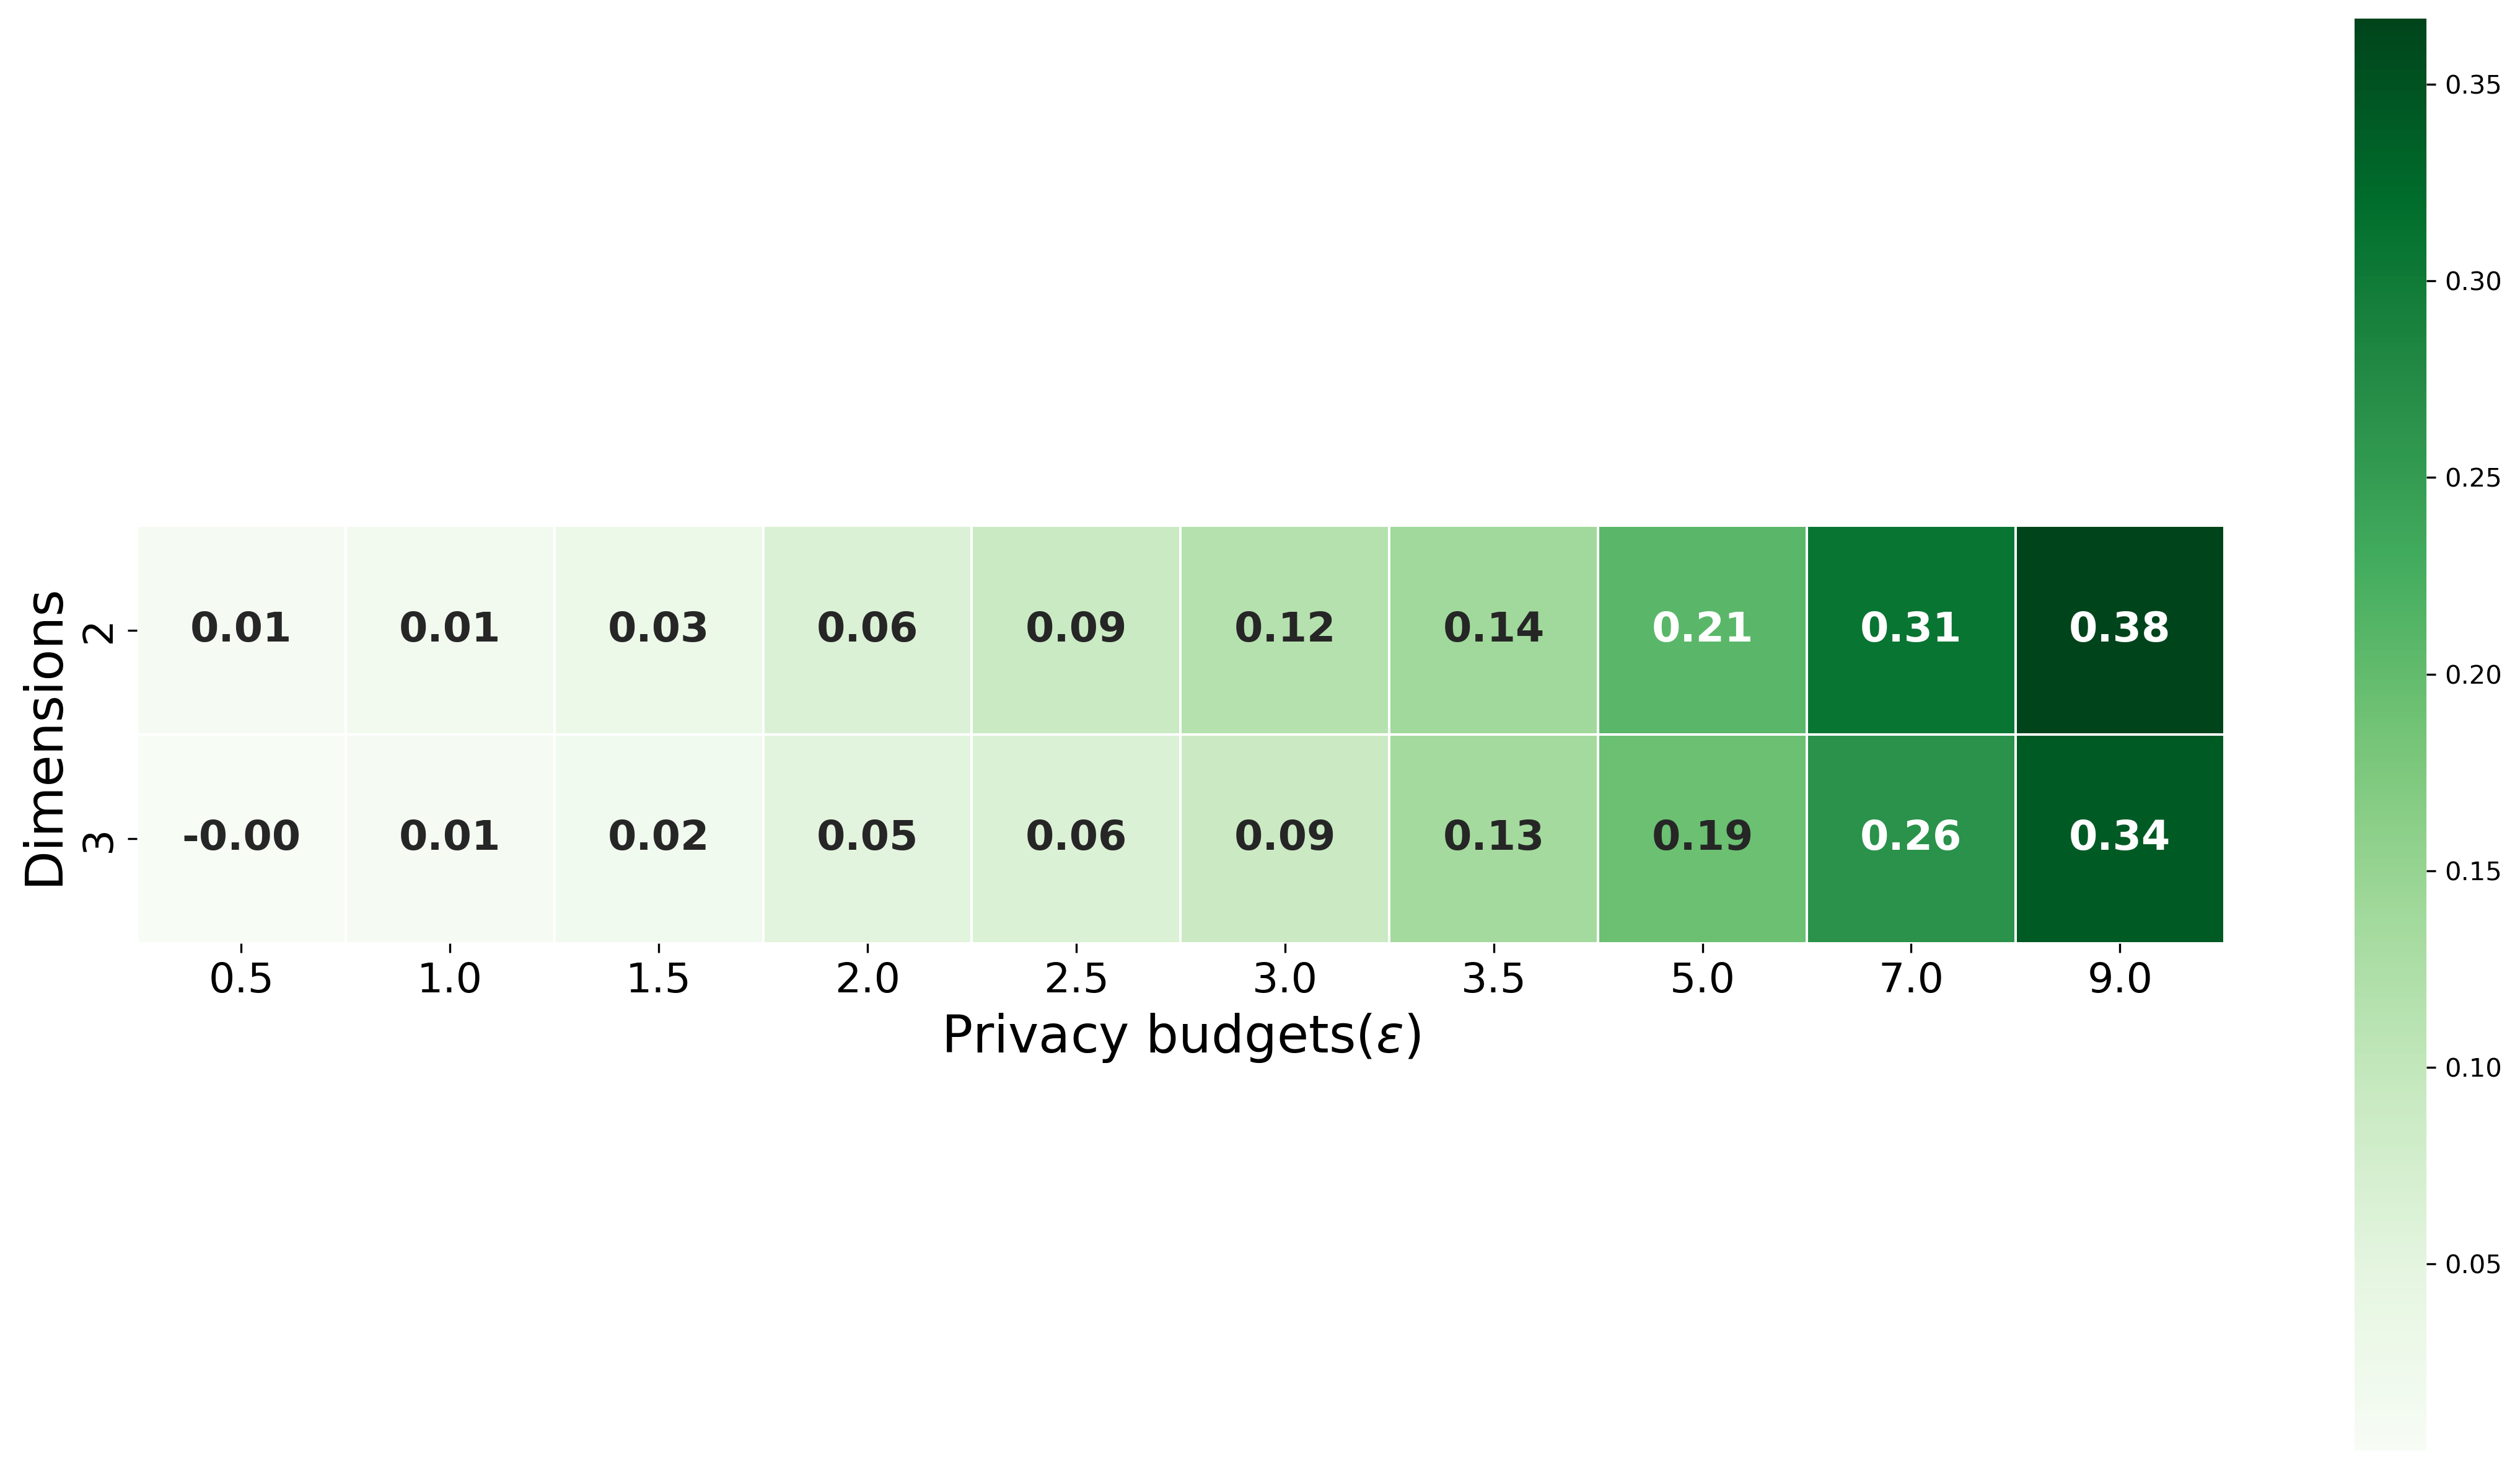
\includegraphics[width=1\textwidth]{Results/nd-laplace/nd-Laplace/circle-dataset/ami.png}
      \label{fig:ami_circle-dataset_comparison_kdlaplace_2d}
    \end{subfigure}
    \vfill % vertical space
    \begin{subfigure}[c]{1\textwidth}
      \caption{\textbf{Adjusted Mutual Information comparison for the Piecewise mechanism}}
      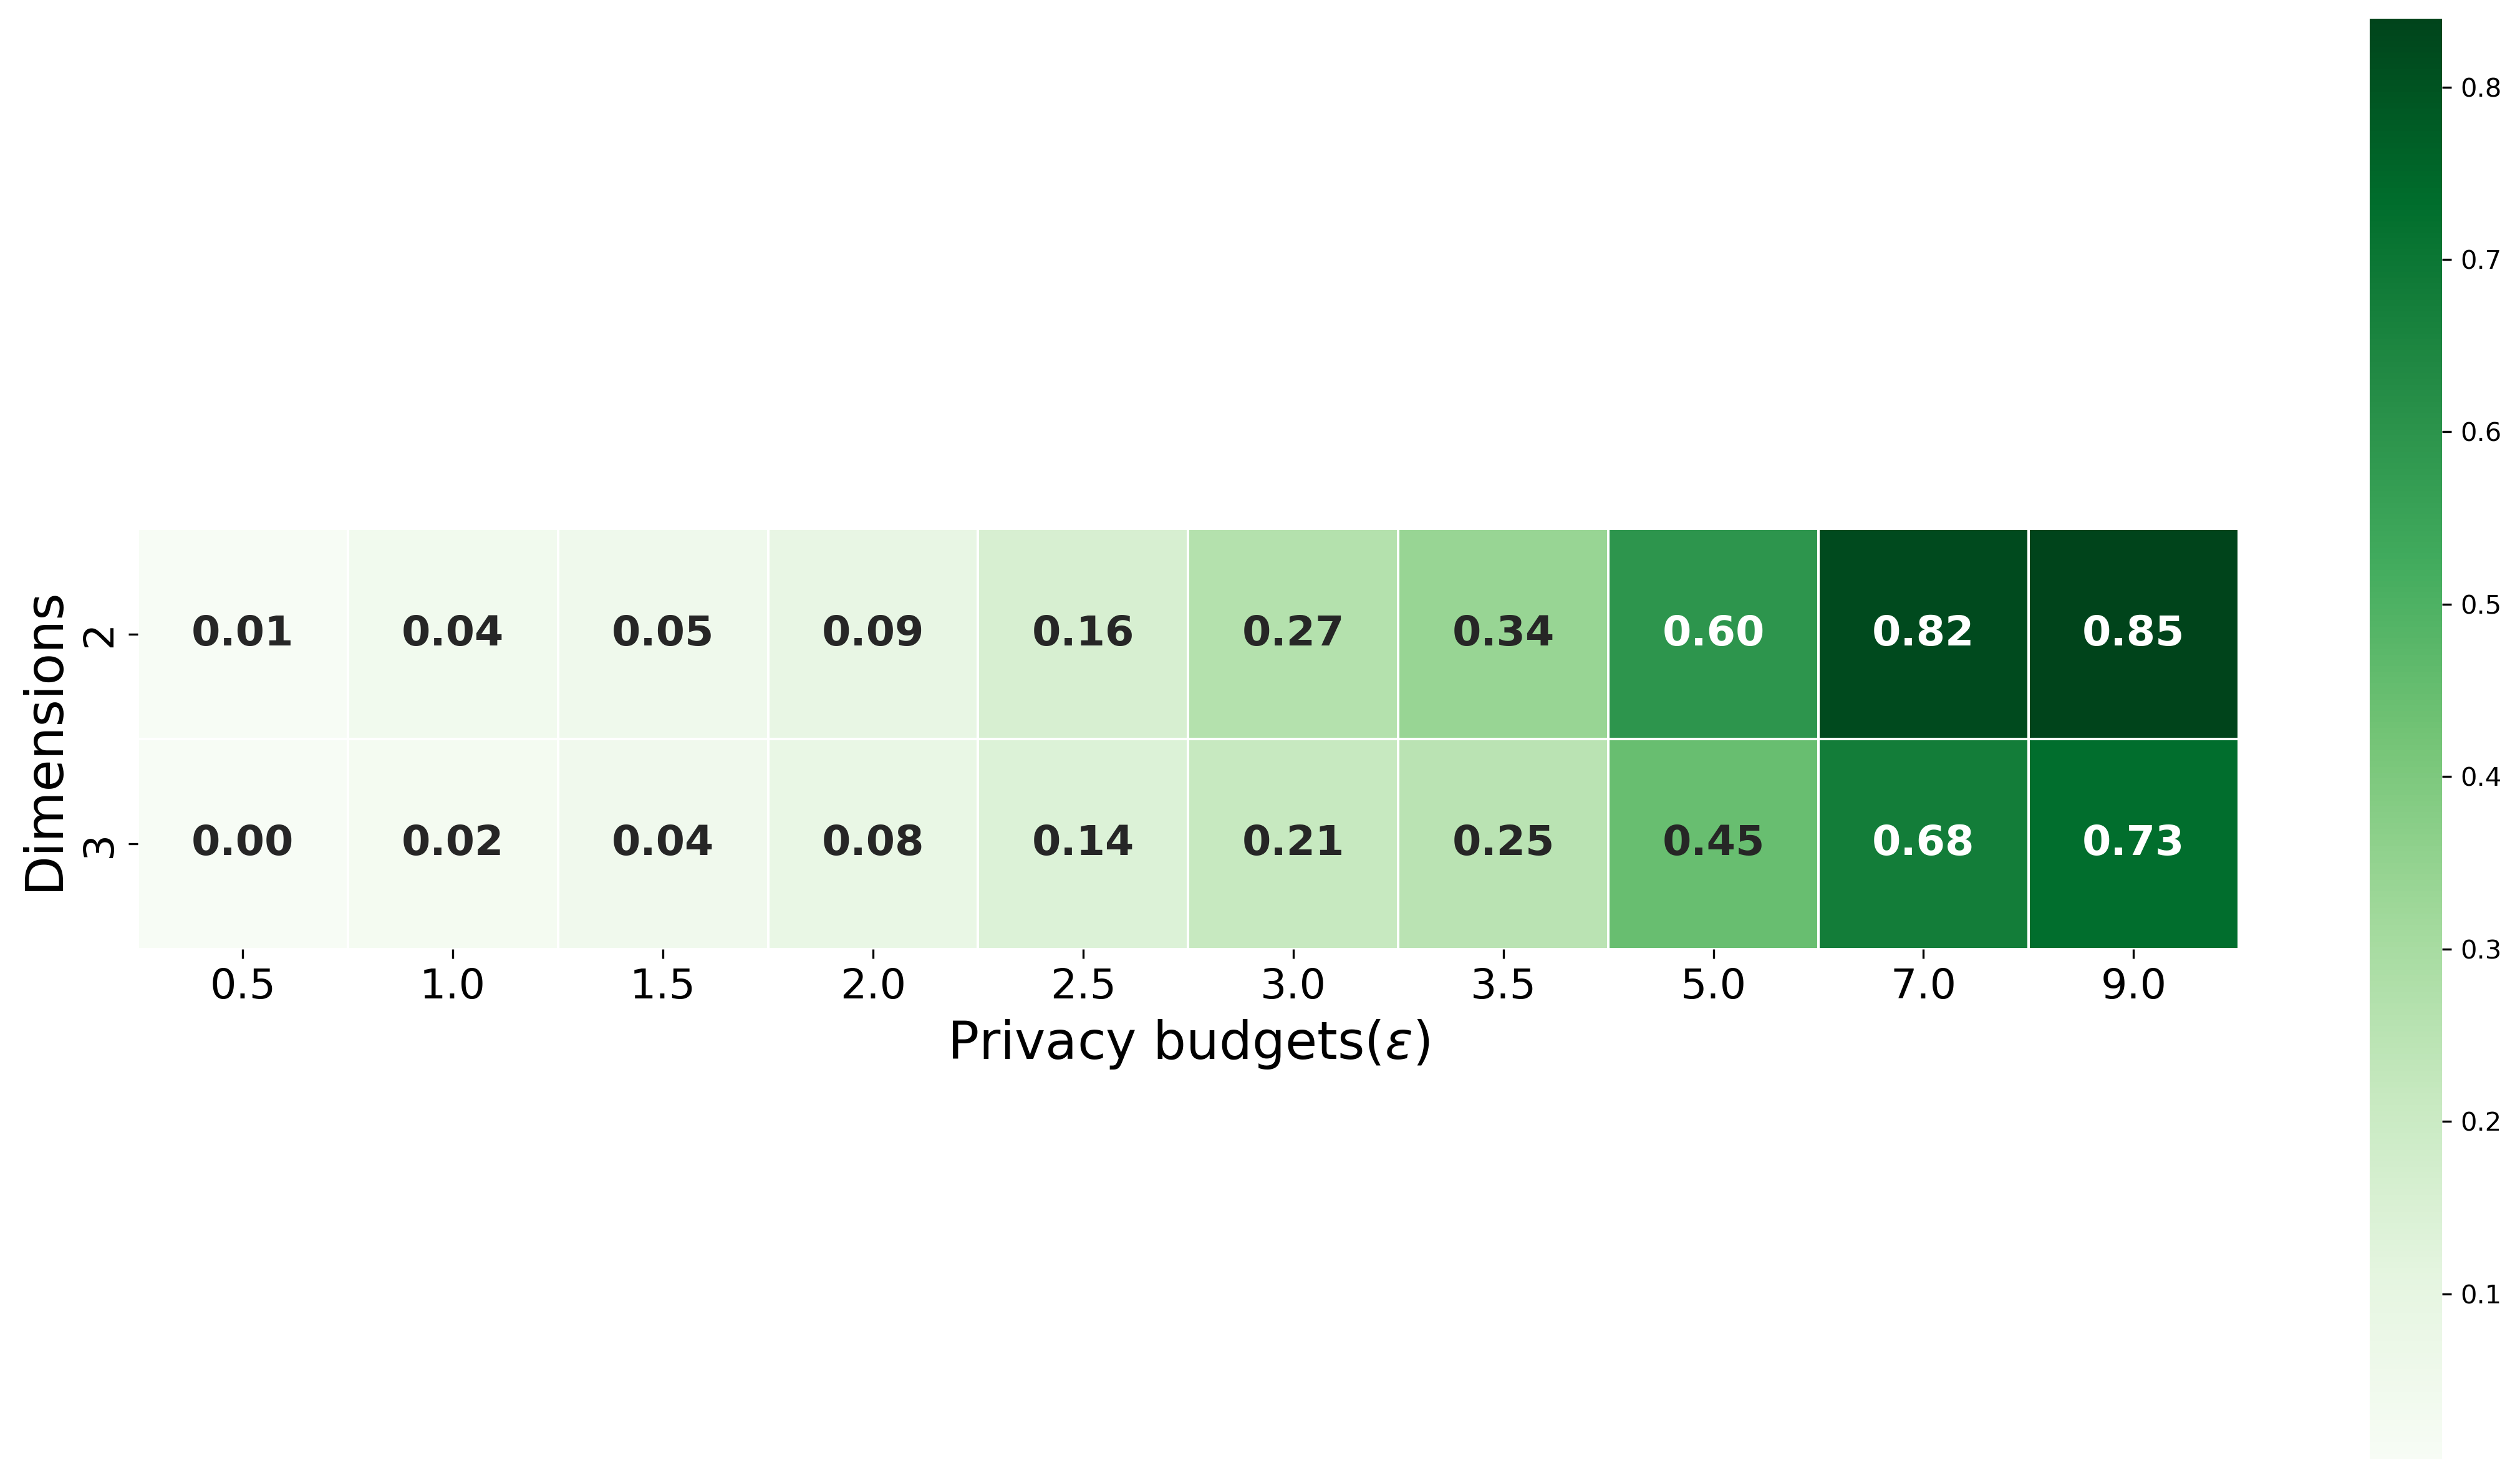
\includegraphics[width=1\textwidth]{Results/nd-laplace/piecewise/circle-dataset/ami.png}
      \label{fig:ami_circle-dataset_comparison_piecewise_2d}
    \end{subfigure}
  \end{subfigure}
\end{figure}

\newpage
\subsection{Line-dataset}
\begin{figure}[H]
  \centering
  \begin{subfigure}[b]{0.85\textwidth}
    \begin{subfigure}[c]{1\textwidth}
      \caption{\textbf{Adjusted Mutual Information comparison for the kd-Laplace mechanism}}
      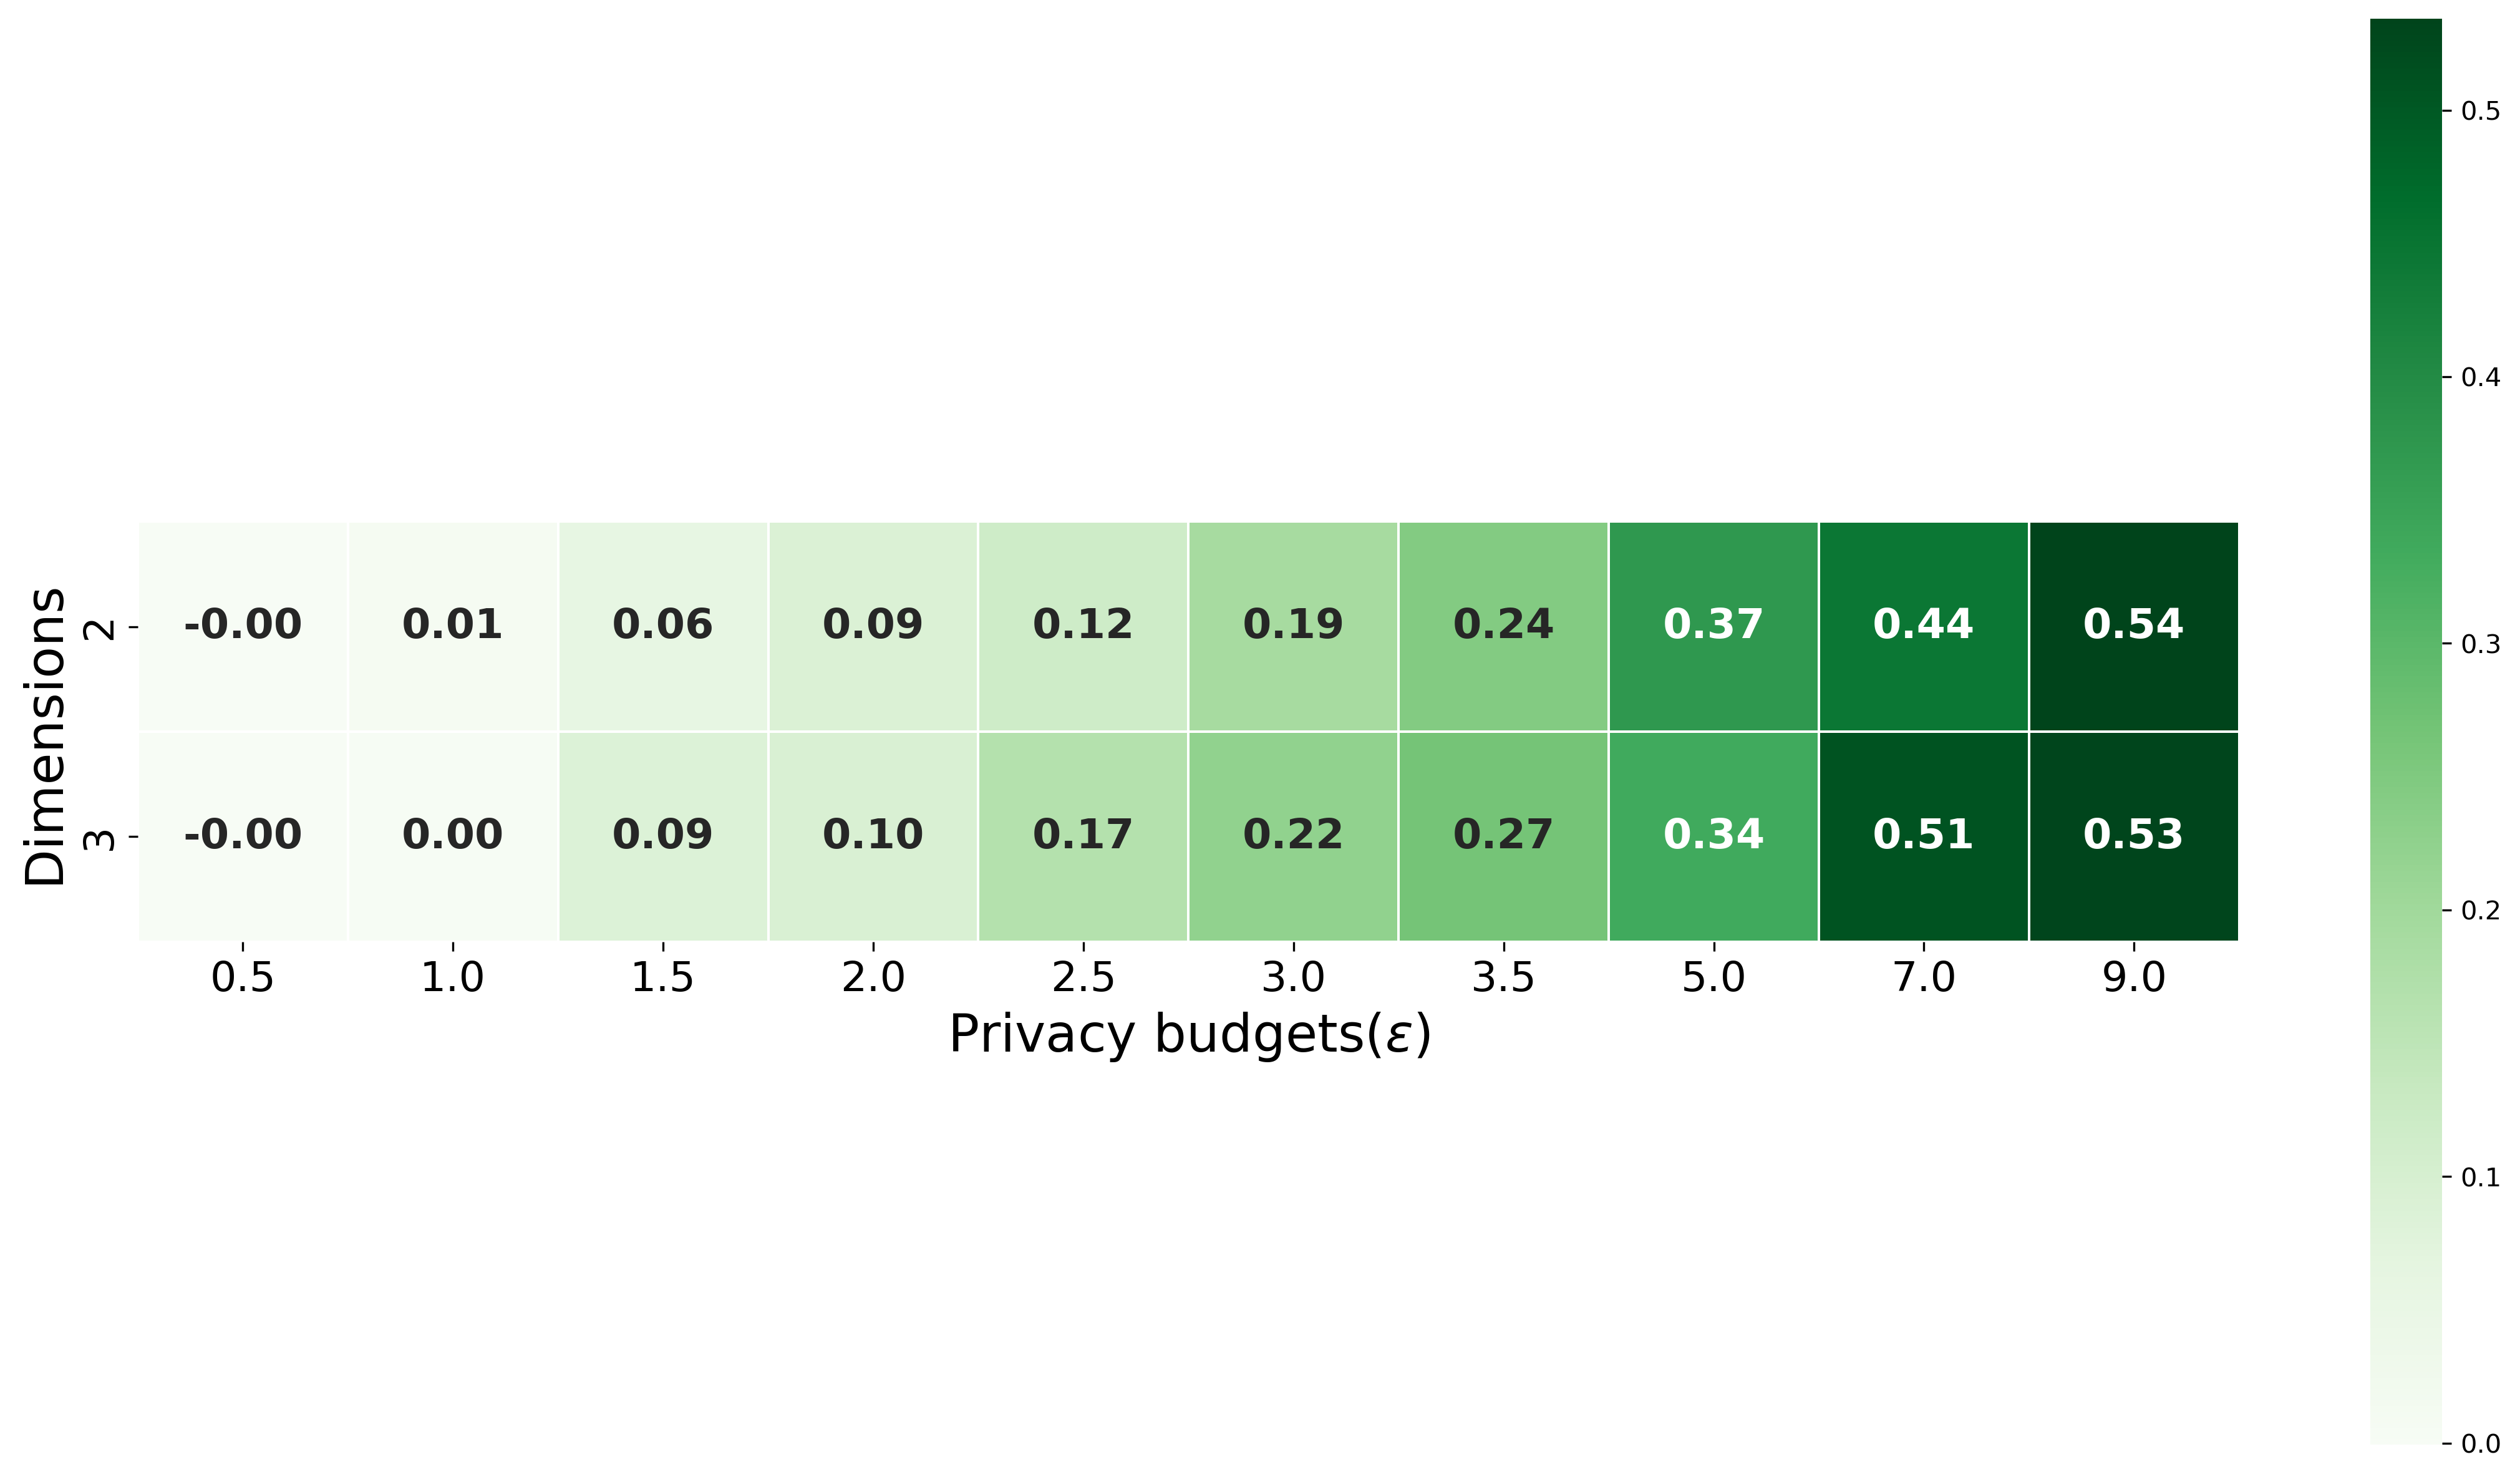
\includegraphics[width=1\textwidth]{Results/nd-laplace/nd-Laplace/line-dataset/ami.png}
      \label{fig:ami_line-dataset_comparison_kdlaplace_2d}
    \end{subfigure}
    \vfill % vertical space
    \begin{subfigure}[c]{1\textwidth}
      \caption{\textbf{Adjusted Mutual Information comparison for the Piecewise mechanism}}
      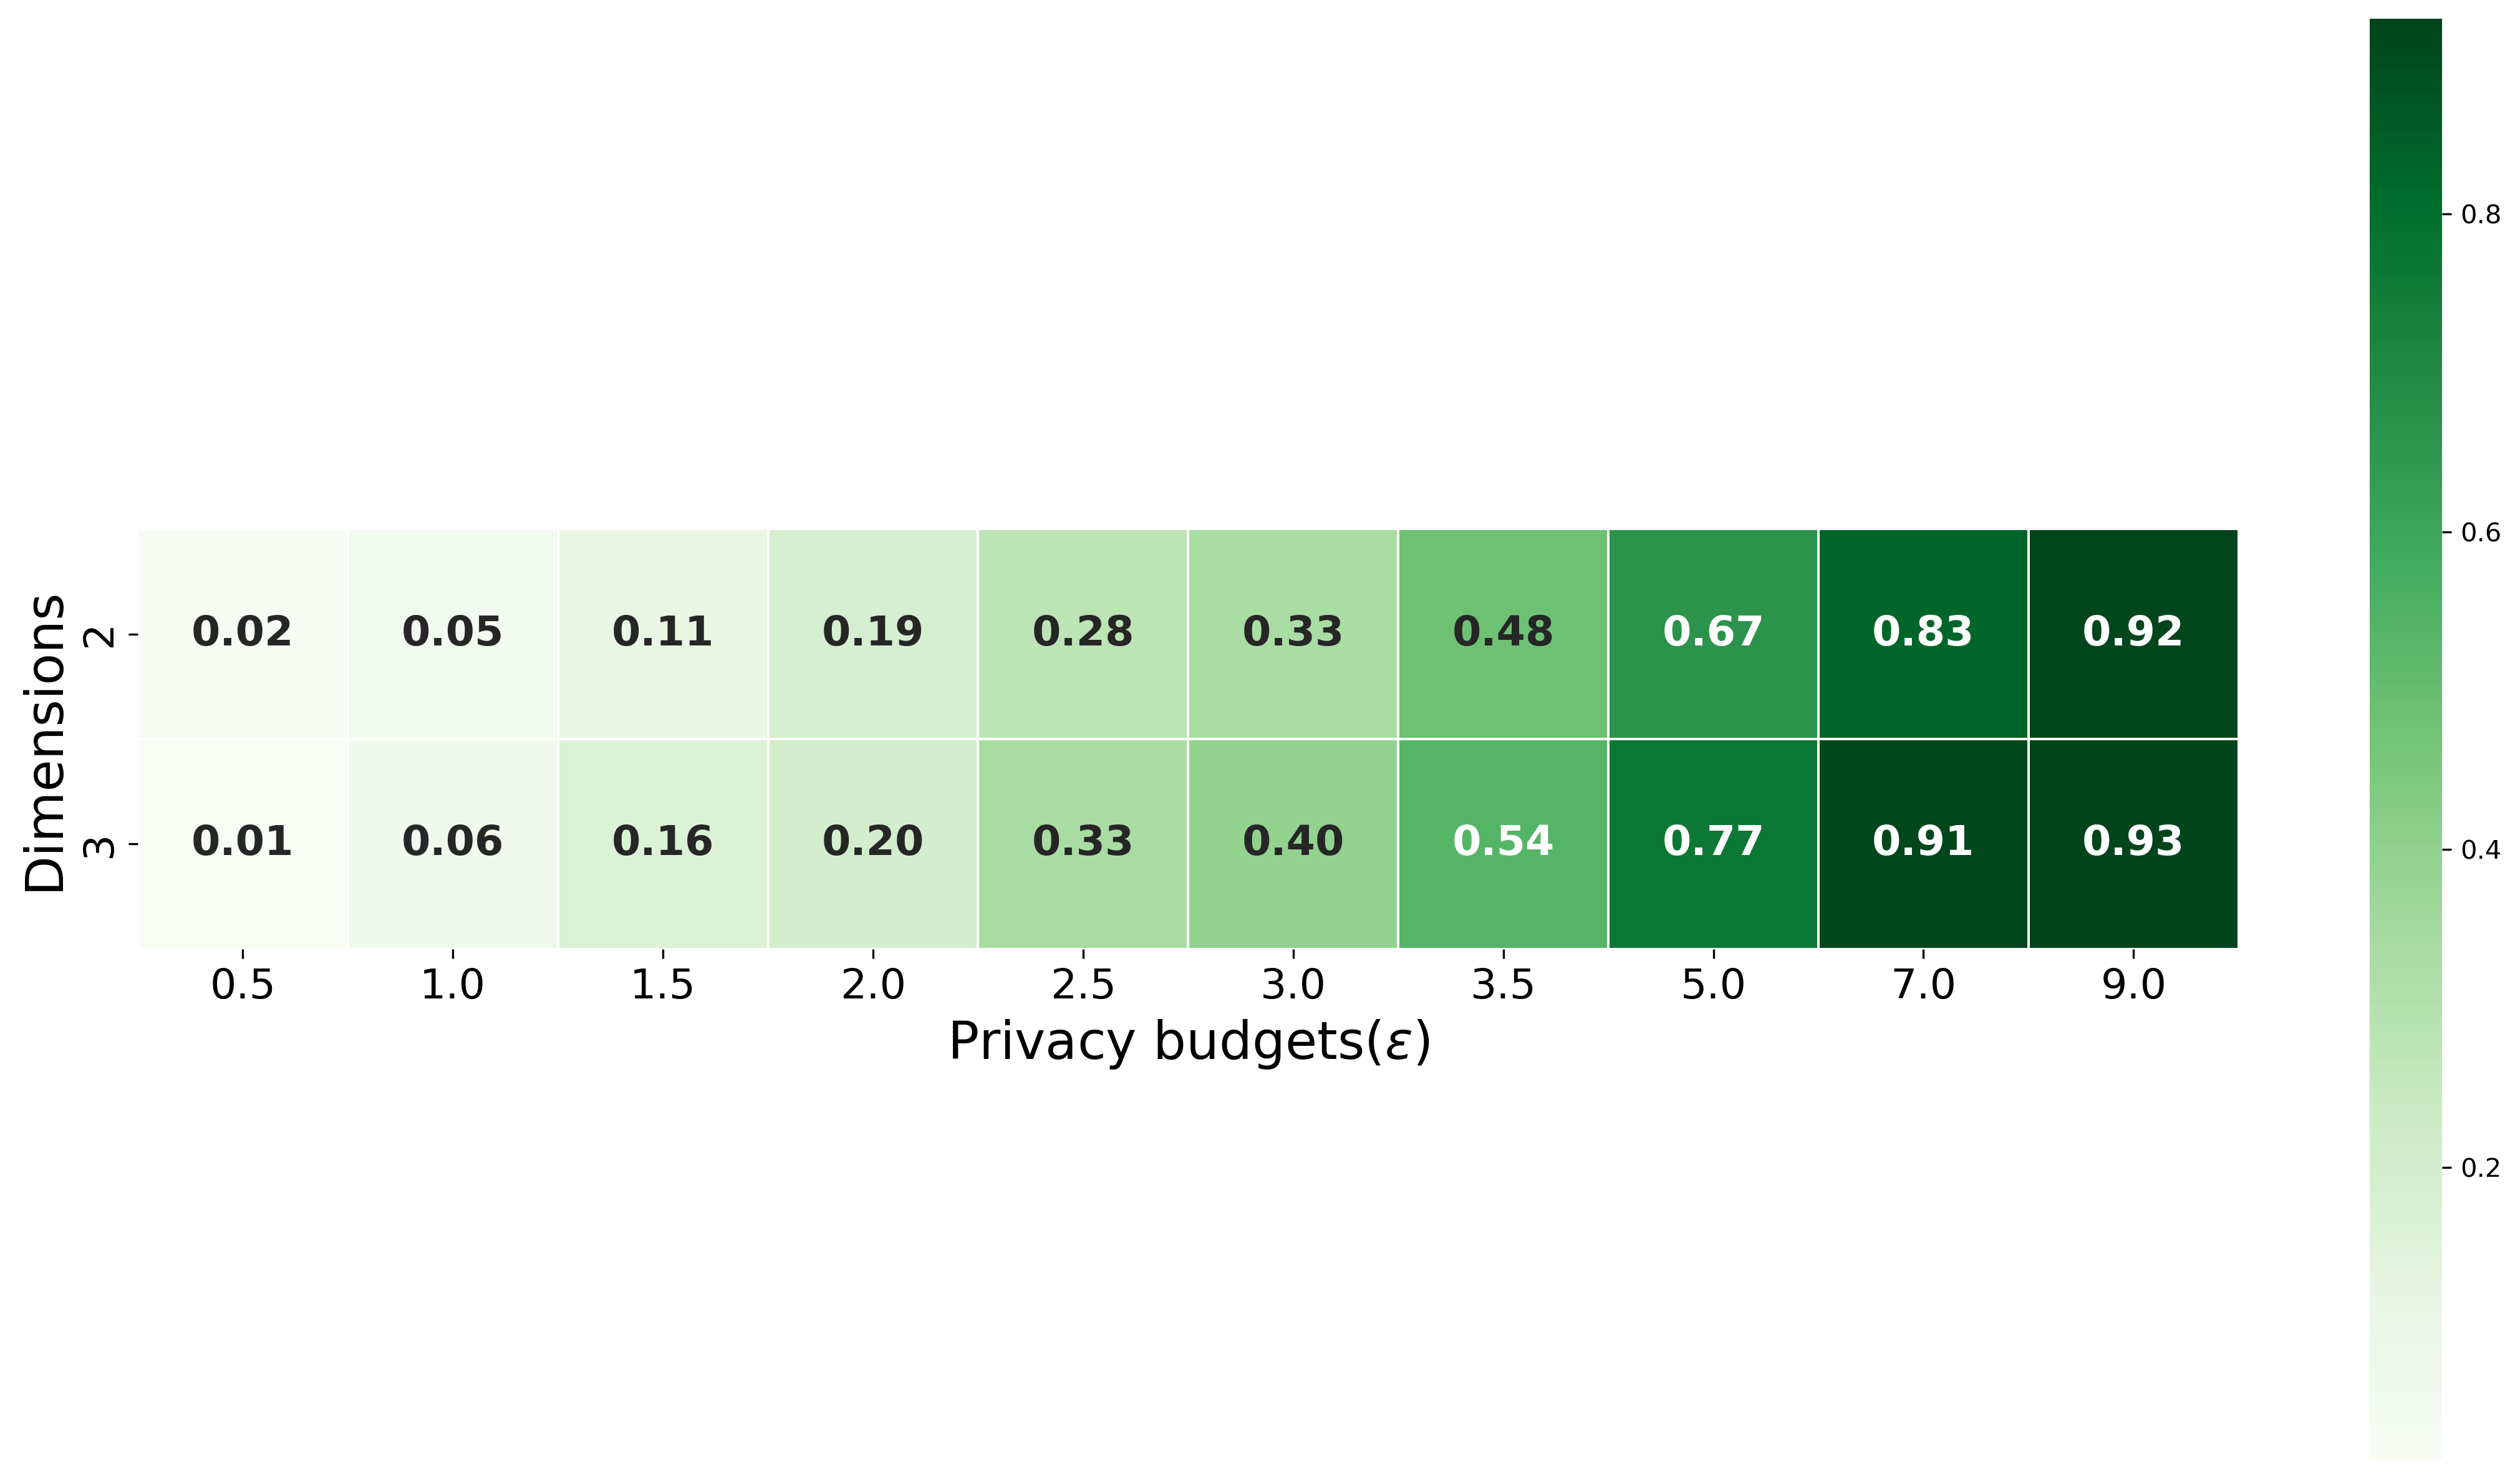
\includegraphics[width=1\textwidth]{Results/nd-laplace/piecewise/line-dataset/ami.png}
      \label{fig:ami_line-dataset_comparison_piecewise_2d}
    \end{subfigure}
  \end{subfigure}
\end{figure}
Up to privacy budget 3.5, the scores remain relatively similar for both mechanisms, but after that, they become better for Piecewise.

For kD-Laplace, the highest score is 0.63 \gls{ami} for privacy budget 9. For privacy budgets 5 and 7, the score is around 0.5 - 0.55. After that, the scores are no higher than 0.37.

Piecewise performs better, with a maximum of 0.90 \gls{ami} for privacy budget 9 for 2 dimensions. For both mechanisms, the dimensions do not significantly impact the score.
\newpage
\subsection{Skewed-dataset}
\begin{figure}[H]
  \centering
  \begin{subfigure}[b]{0.85\textwidth}
    \begin{subfigure}[c]{1\textwidth}
      \caption{\textbf{Adjusted Mutual Information comparison for the kd-Laplace mechanism}}
      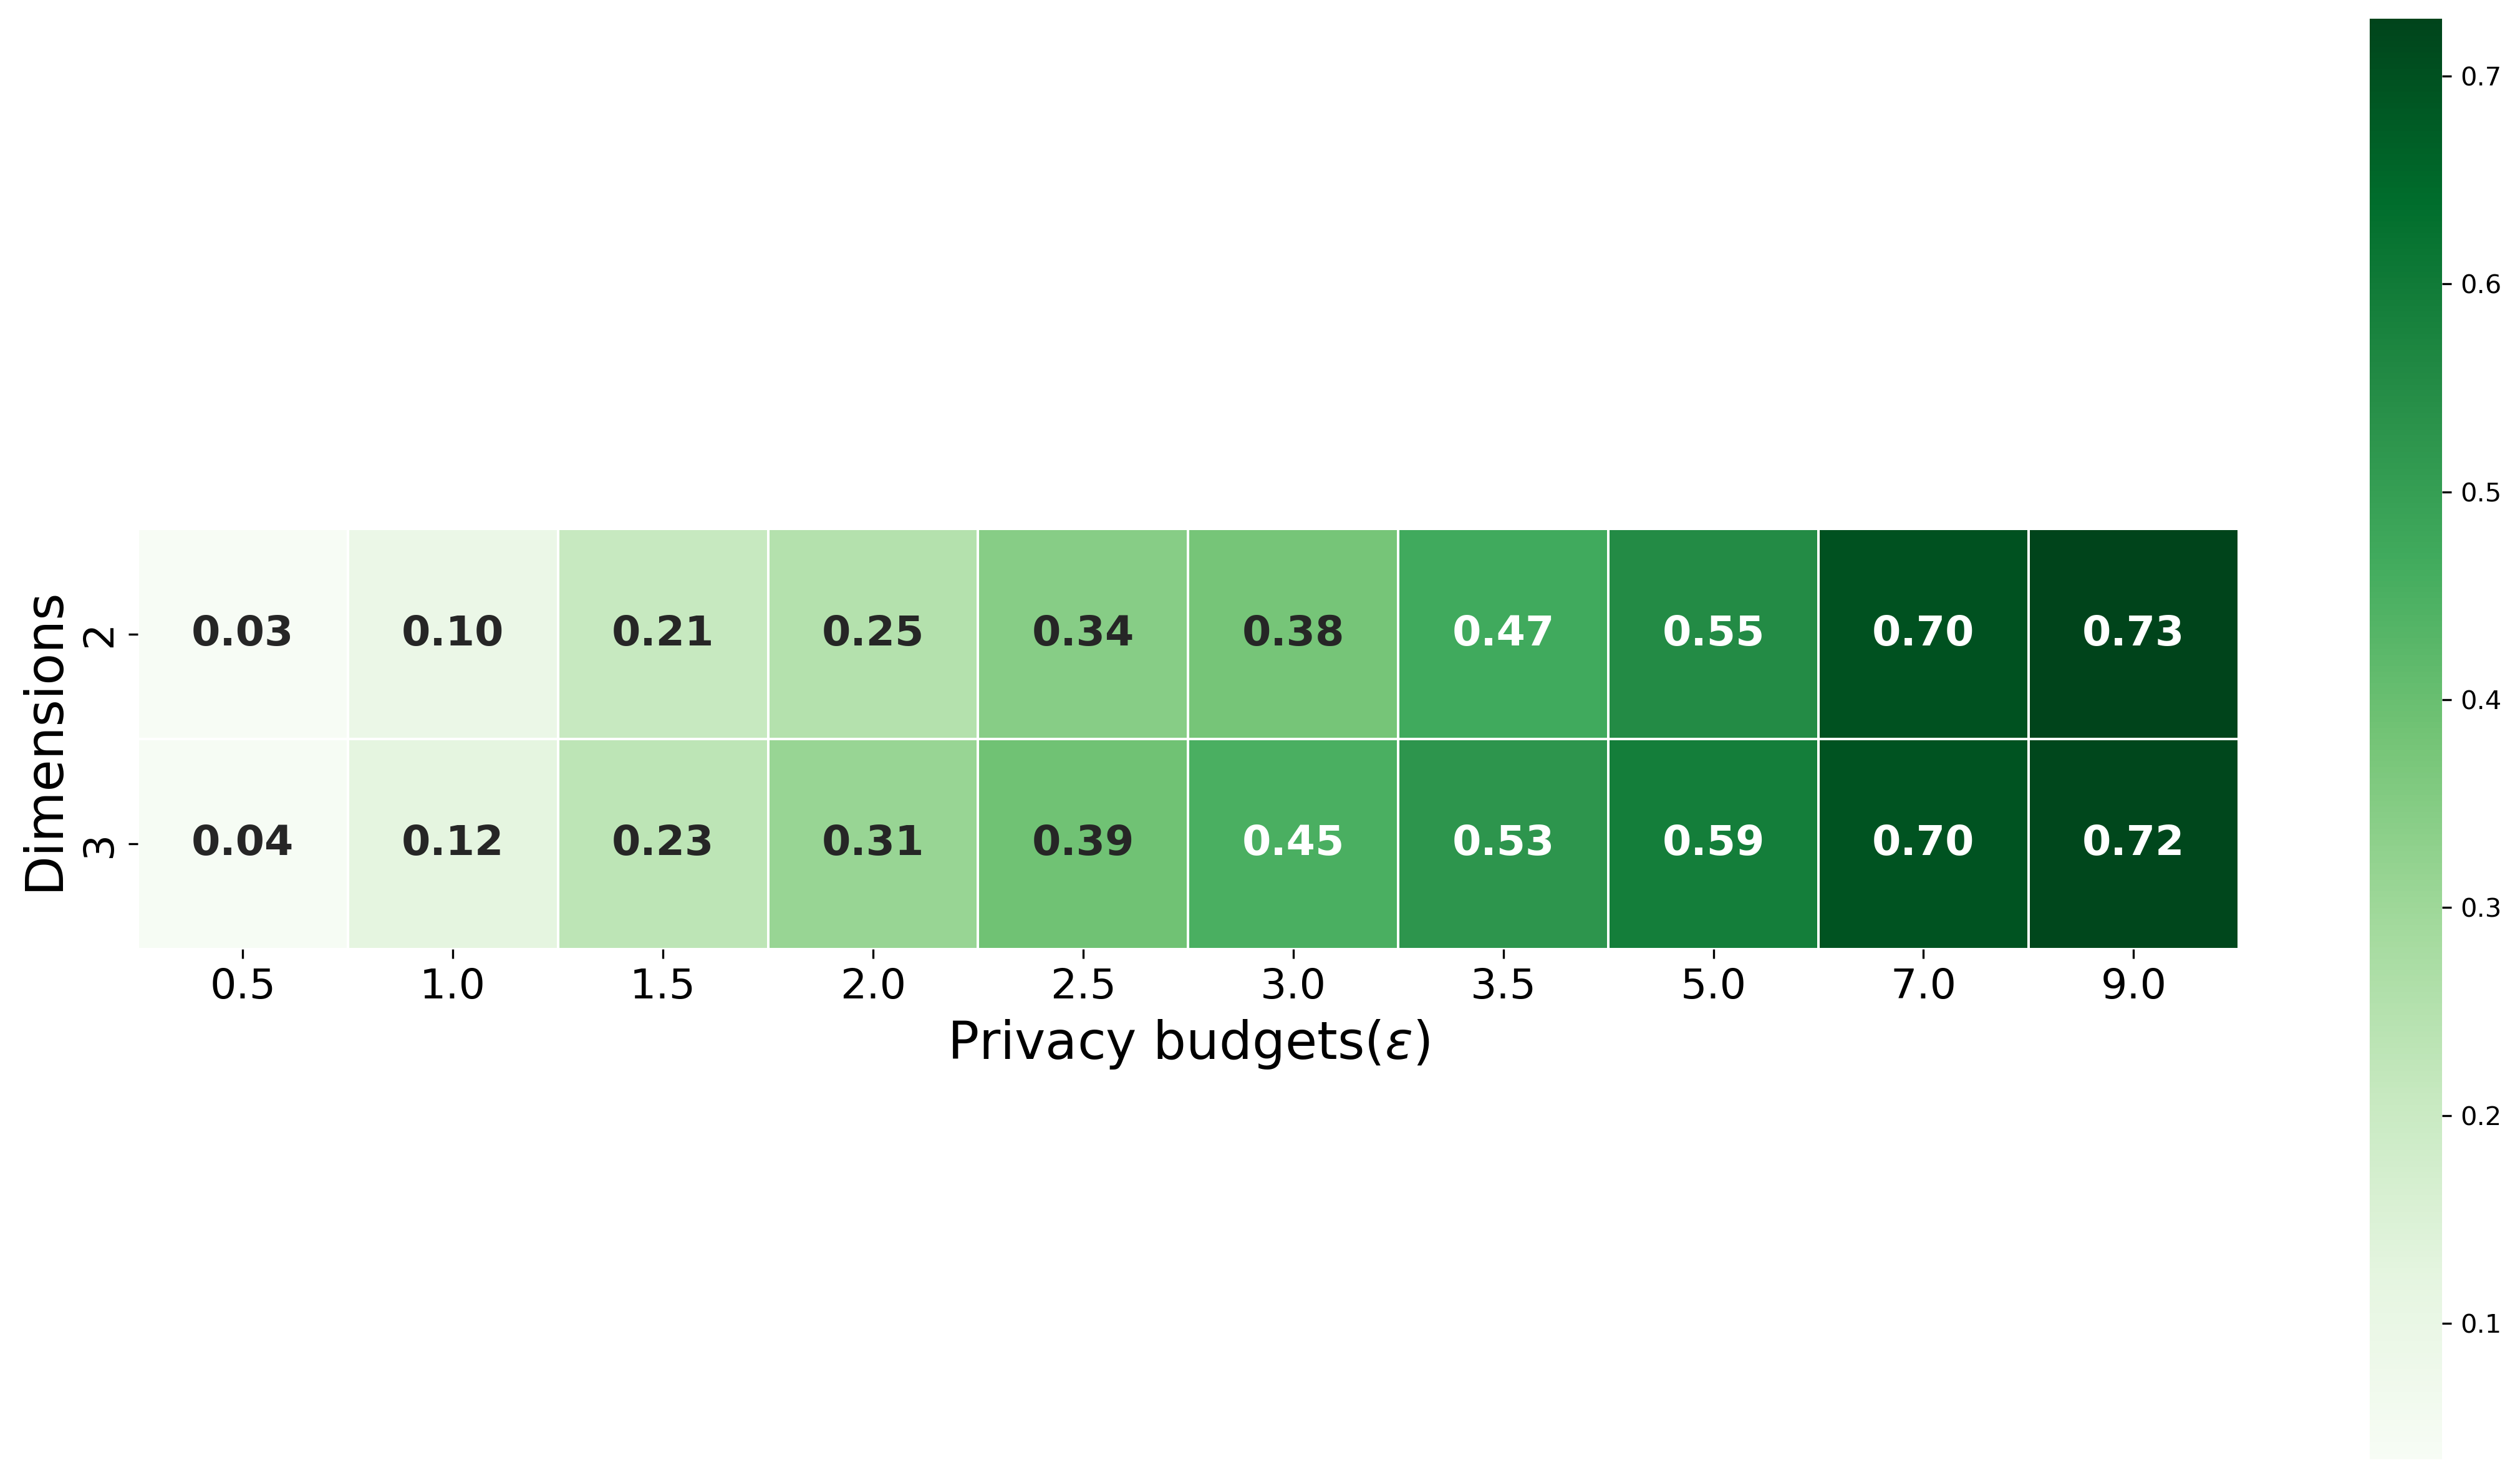
\includegraphics[width=1\textwidth]{Results/nd-laplace/nd-Laplace/skewed-dataset/ami.png}
      \label{fig:ami_skewed-dataset_comparison_kdlaplace_2d}
    \end{subfigure}
    \vfill % vertical space
    \begin{subfigure}[c]{1\textwidth}
      \caption{\textbf{Adjusted Mutual Information comparison for the Piecewise mechanism}}
      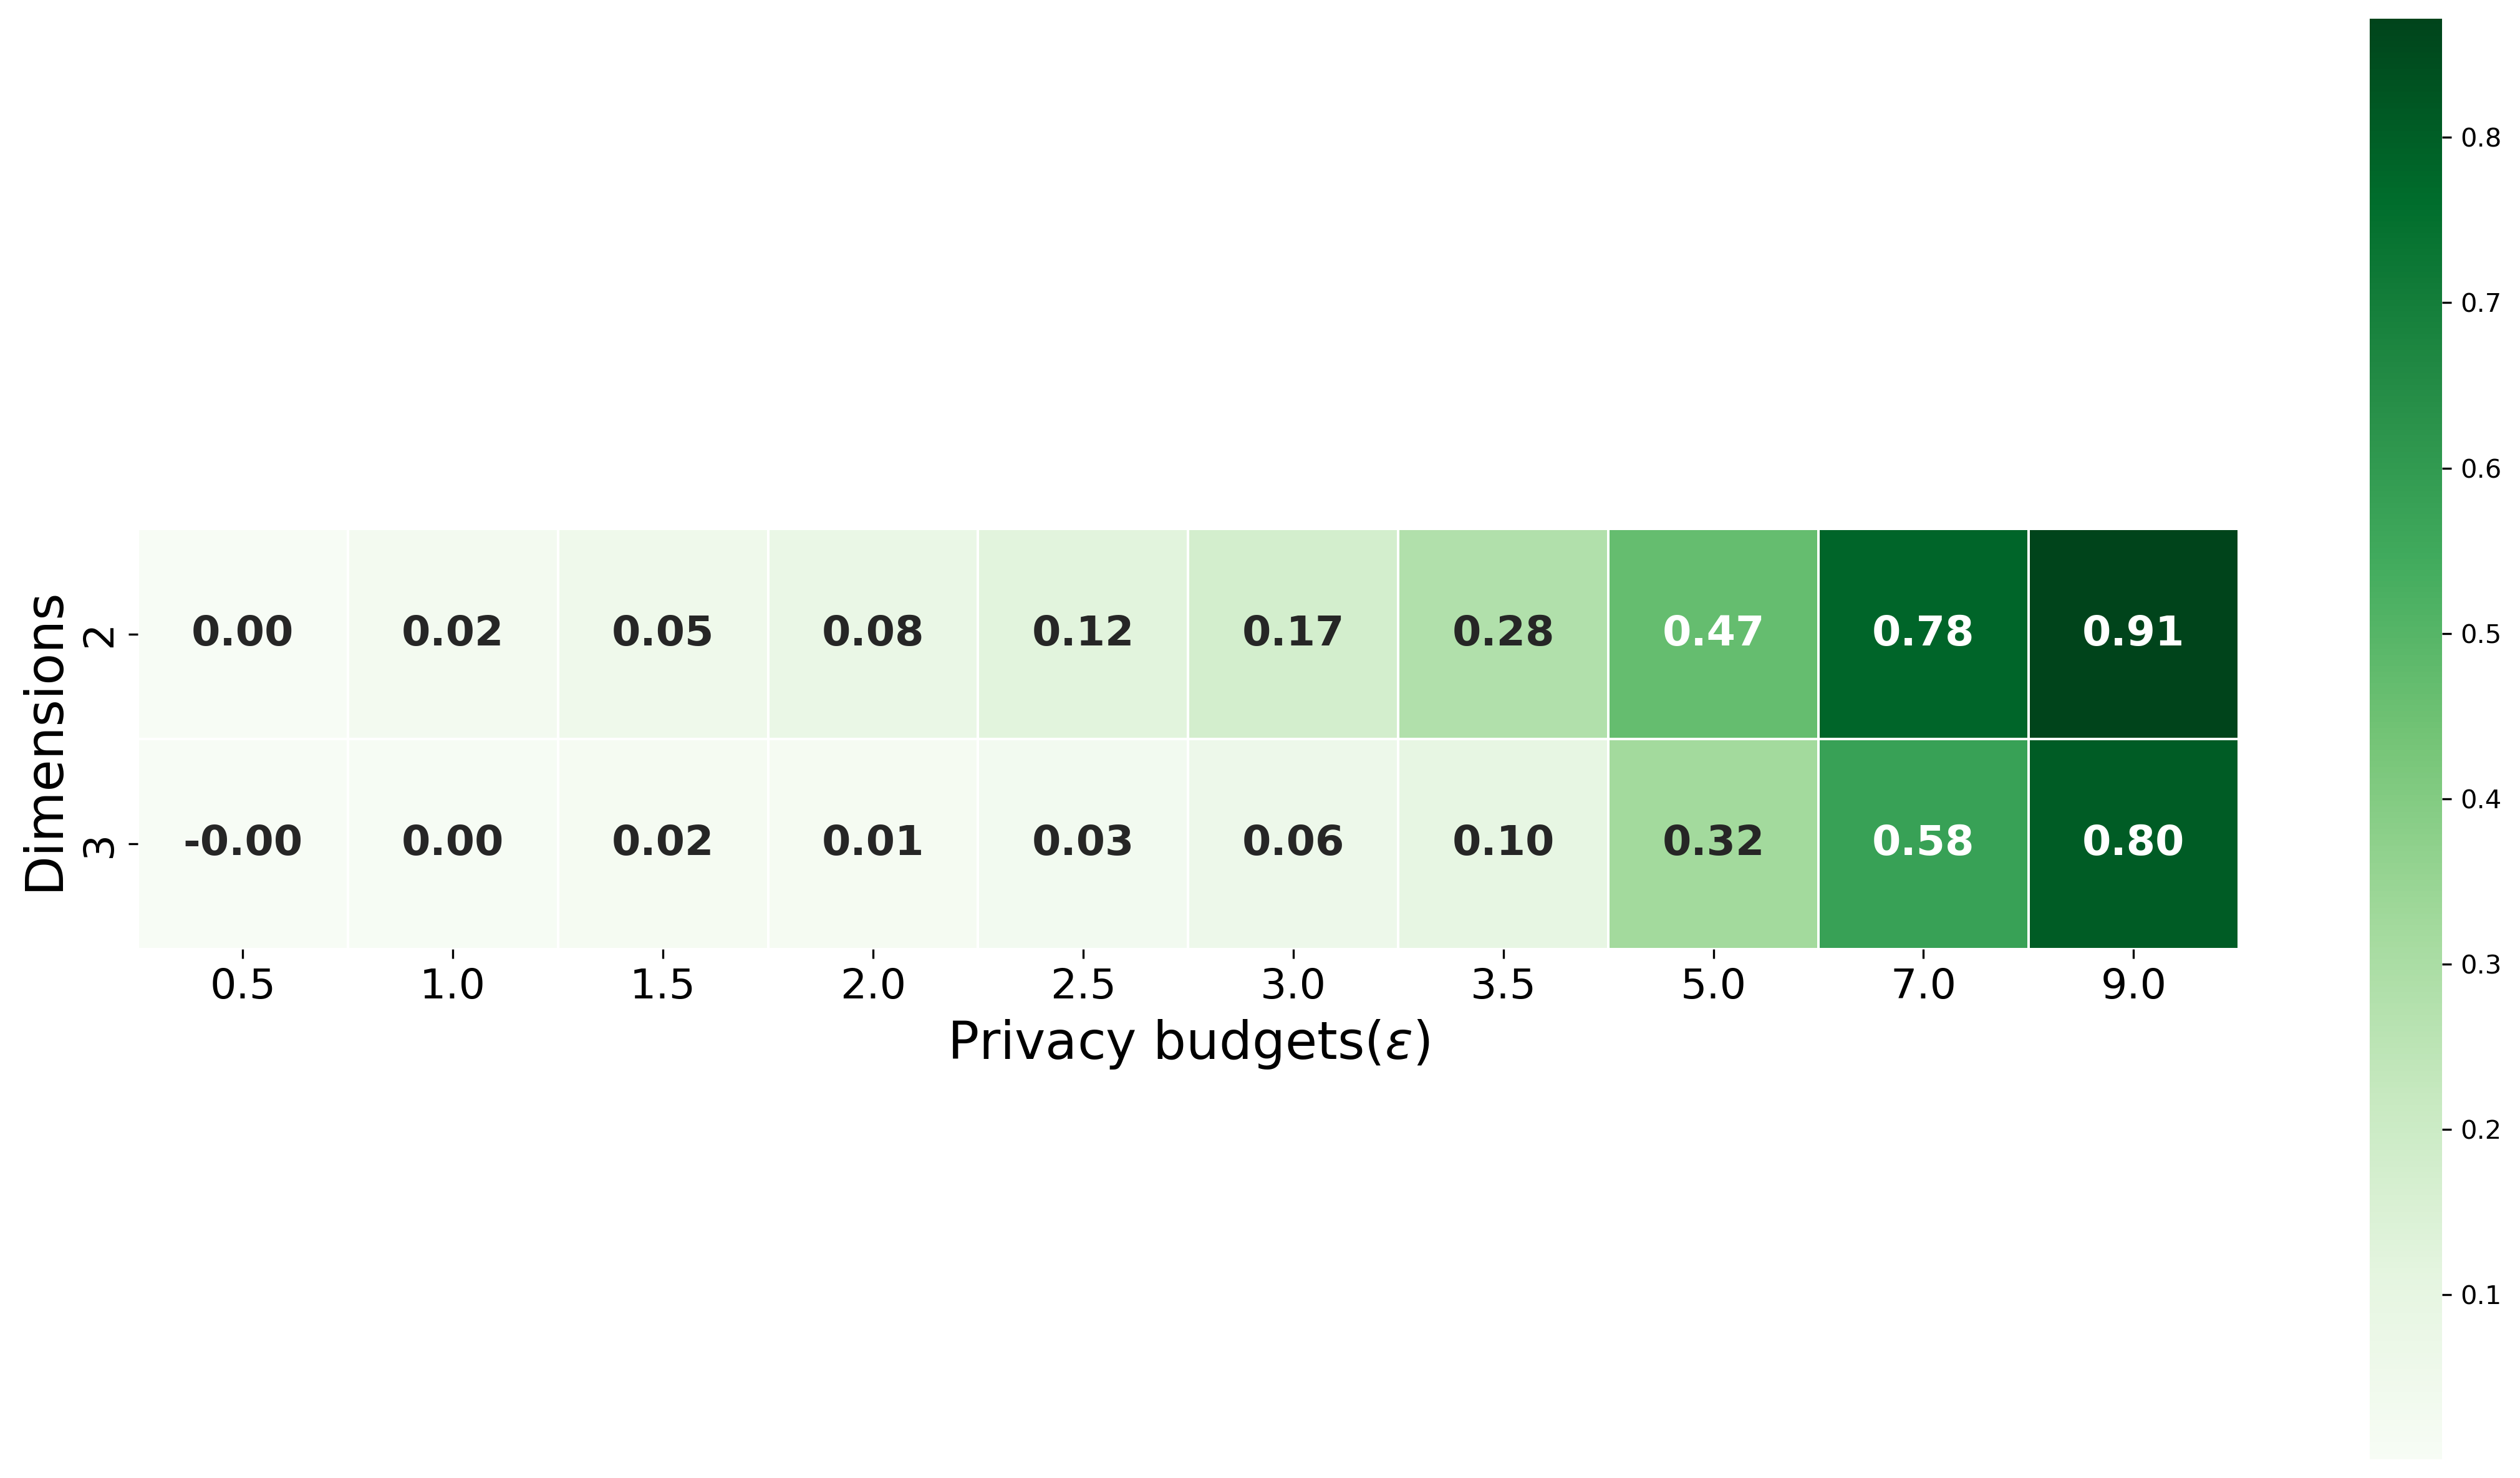
\includegraphics[width=1\textwidth]{Results/nd-laplace/piecewise/skewed-dataset/ami.png}
      \label{fig:ami_skewed-dataset_comparison_piecewise_2d}
    \end{subfigure}
  \end{subfigure}
\end{figure}
The kD-Laplace mechanism performs slightly better from privacy budgets 2 to 5. However, Piecewise performs significantly better after that, achieving around 0.73 and 0.85 \gls{ami} for privacy budgets 7 and 9, respectively.

In contrast, kD-Laplace scores much lower in this range. Furthermore, it appears that the dimensions do not significantly impact the performance of the mechanisms in this context.
\newpage
}

\section{Privacy}
The sections below present a heatmap comparison of the nd-Laplace and Piecewise mechanisms.
We employed a heatmap to simultaneously depict the privacy budget (epsilon), the number of dimensions, and a specific metric. The metrics we use for this are the Membership advantage, \gls{tpr} and privacy distance. 

On the heatmap, the x-axis represents the privacy budget, while the y-axis illustrates the number of dimensions. Each cell of the heatmap displays the specific metric value. The intensity of the cell's color corresponds to the \gls{ami} score: a darker shade signifies a higher score:
\begin{enumerate}
    \item  For the membership advantage and \gls{tpr}, a lighter cell color (lower value) indicates a better score.
    \item For the privacy distance, the opposite is true; if the cell color is dark (high value), it provides more distance and thus more privacy.
\end{enumerate}
%The images below display bar plots for the membership advantage and TPR of membership inference attacks as described in the methodology.
%We use the same color scheme in the previous section to display the different mechanisms.
%In addition, a red line was drawn to indicate the baseline TPR (the non-private dataset's TPR). \newline
\newpage
\subsection{Seeds dataset}
\begin{figure}[H]
  \centering
  \begin{subfigure}[b]{0.75\textwidth}
    \begin{subfigure}[c]{1\textwidth}
      \caption{\textbf{Heatmap showing membership advantage for the kD-Laplace mechanism, per privacy budget \& dimension for seeds-dataset.}}
      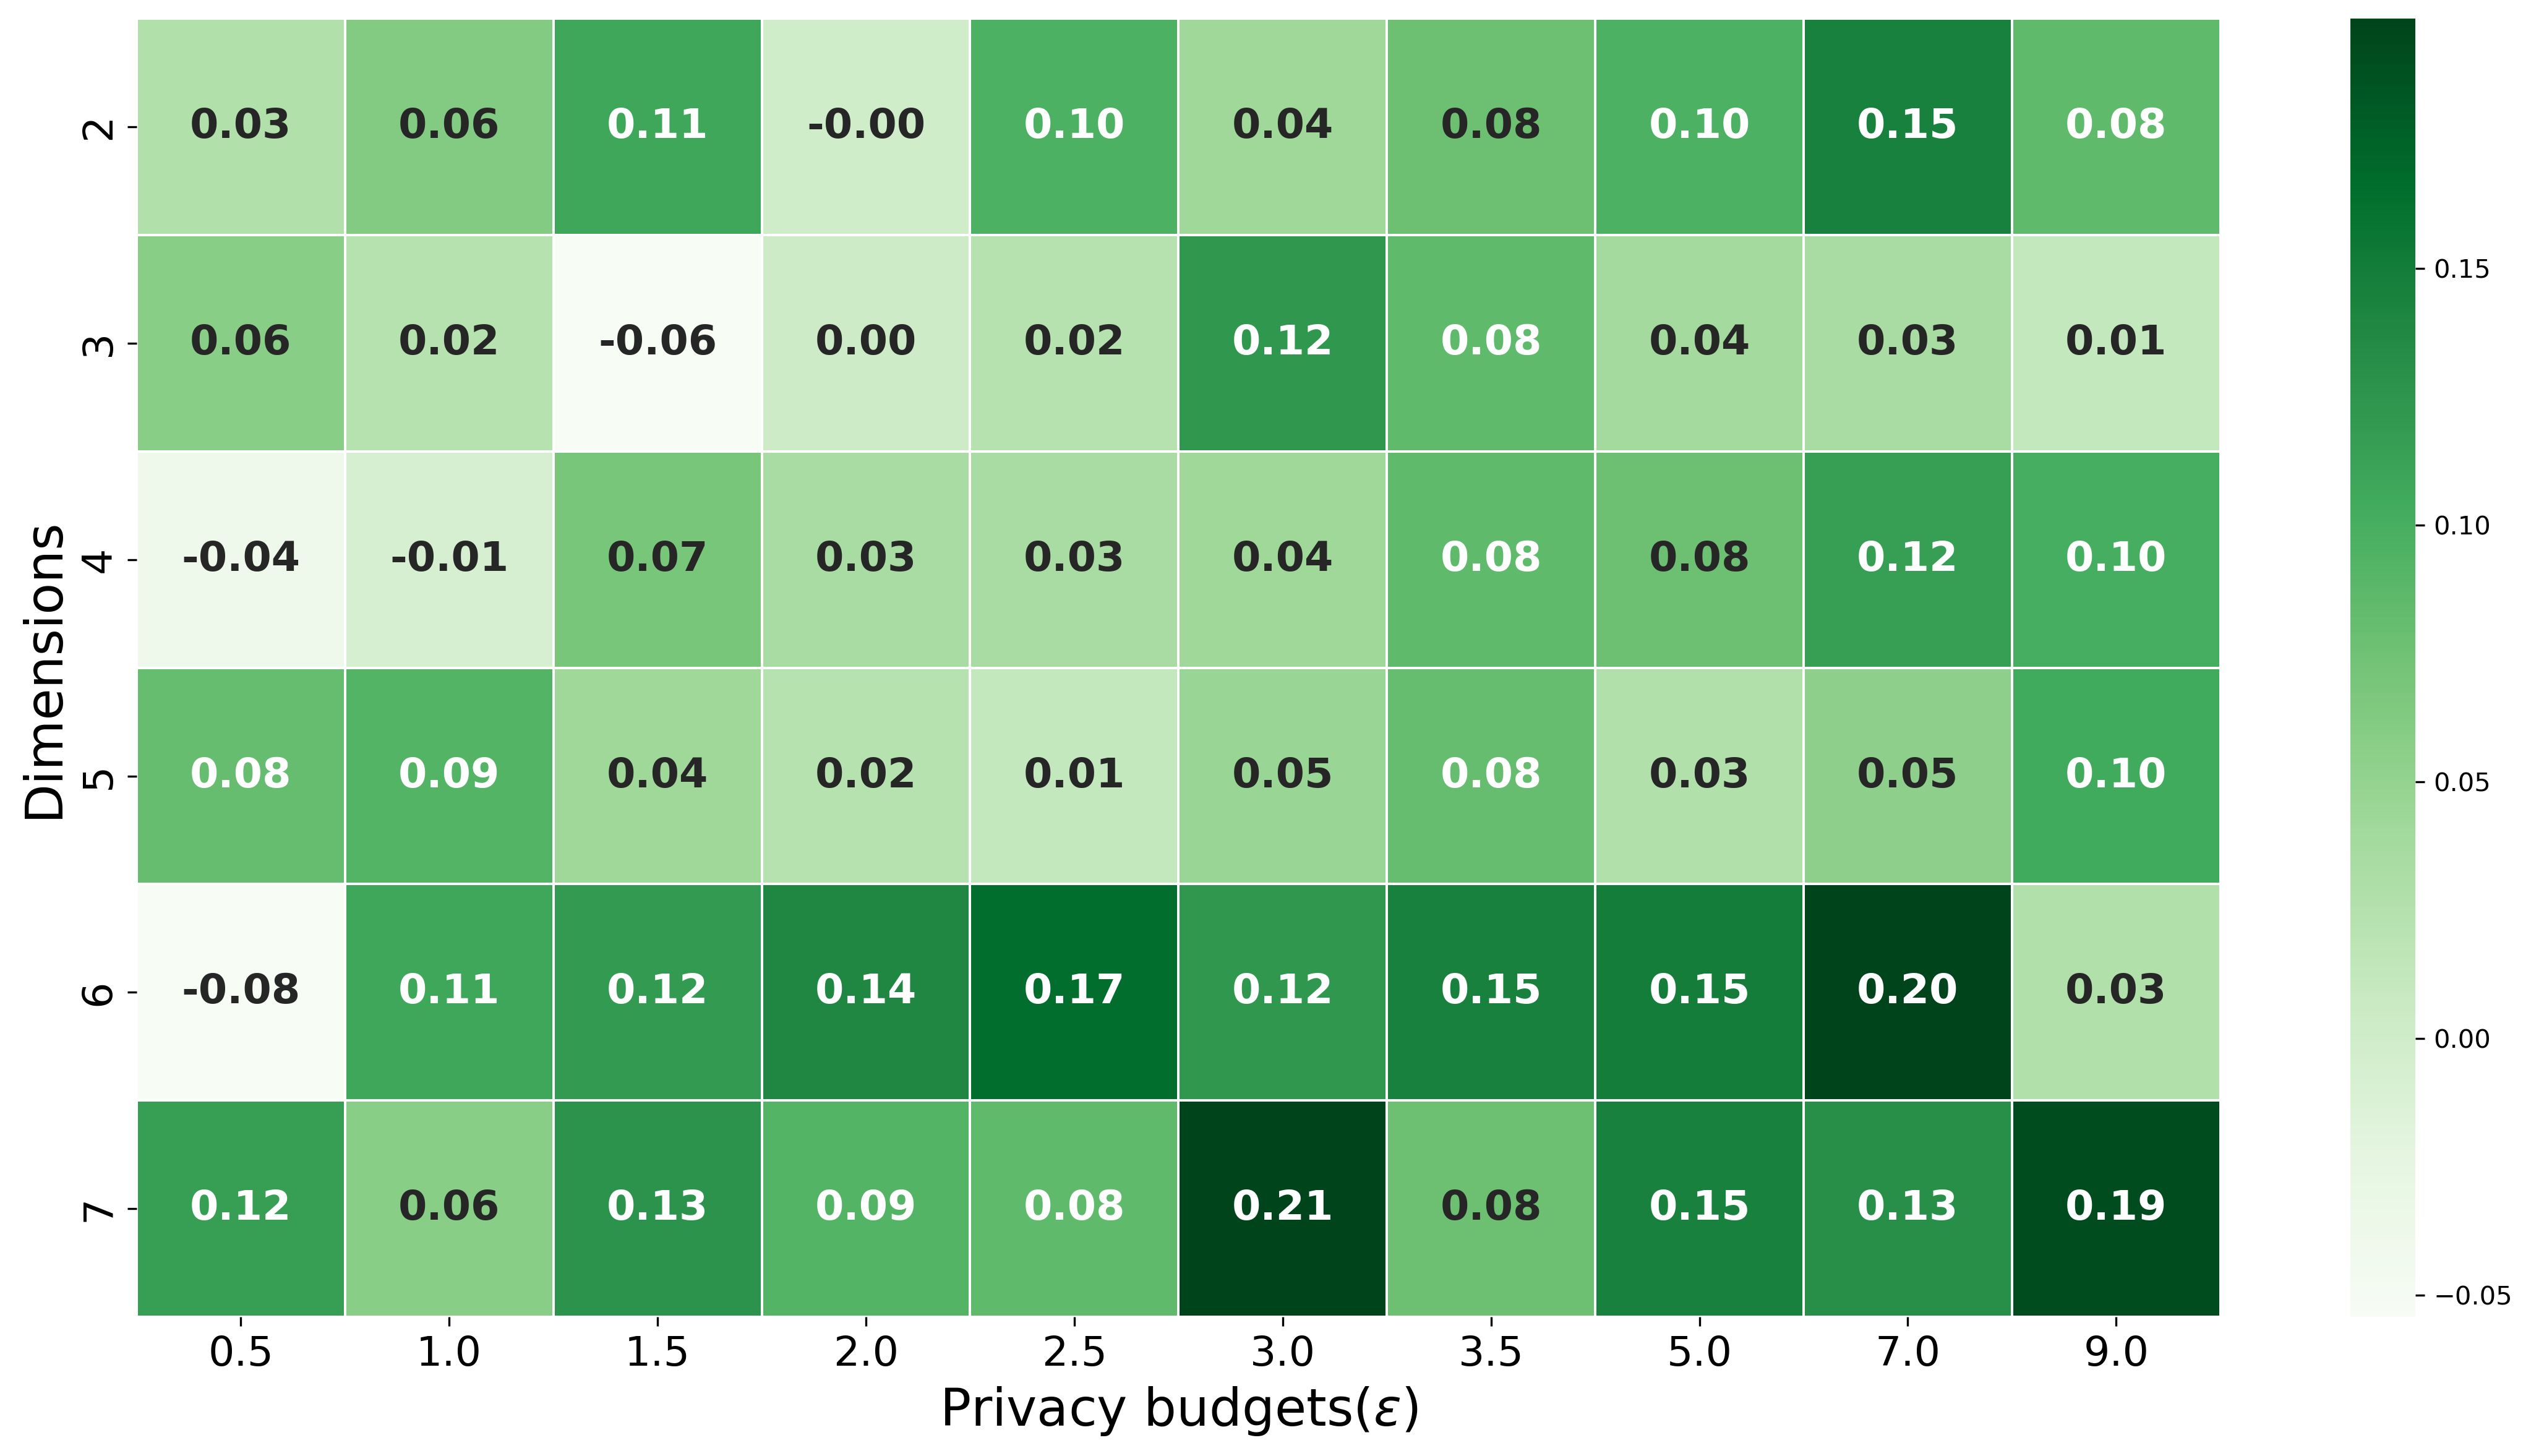
\includegraphics[width=1\textwidth]{Results/nd-laplace/nd-Laplace/seeds-dataset/attack_adv.png}
      \label{fig:privacy_seeds-dataset_adversial_advantage_kd-laplace}
    \end{subfigure}
    \vfill % vertical space

    \begin{subfigure}[c]{1\textwidth}
      \caption{\textbf{Heatmap showing adversary advantage for the Piecewise mechanism, per privacy budget \& dimension for seeds-dataset.}}
      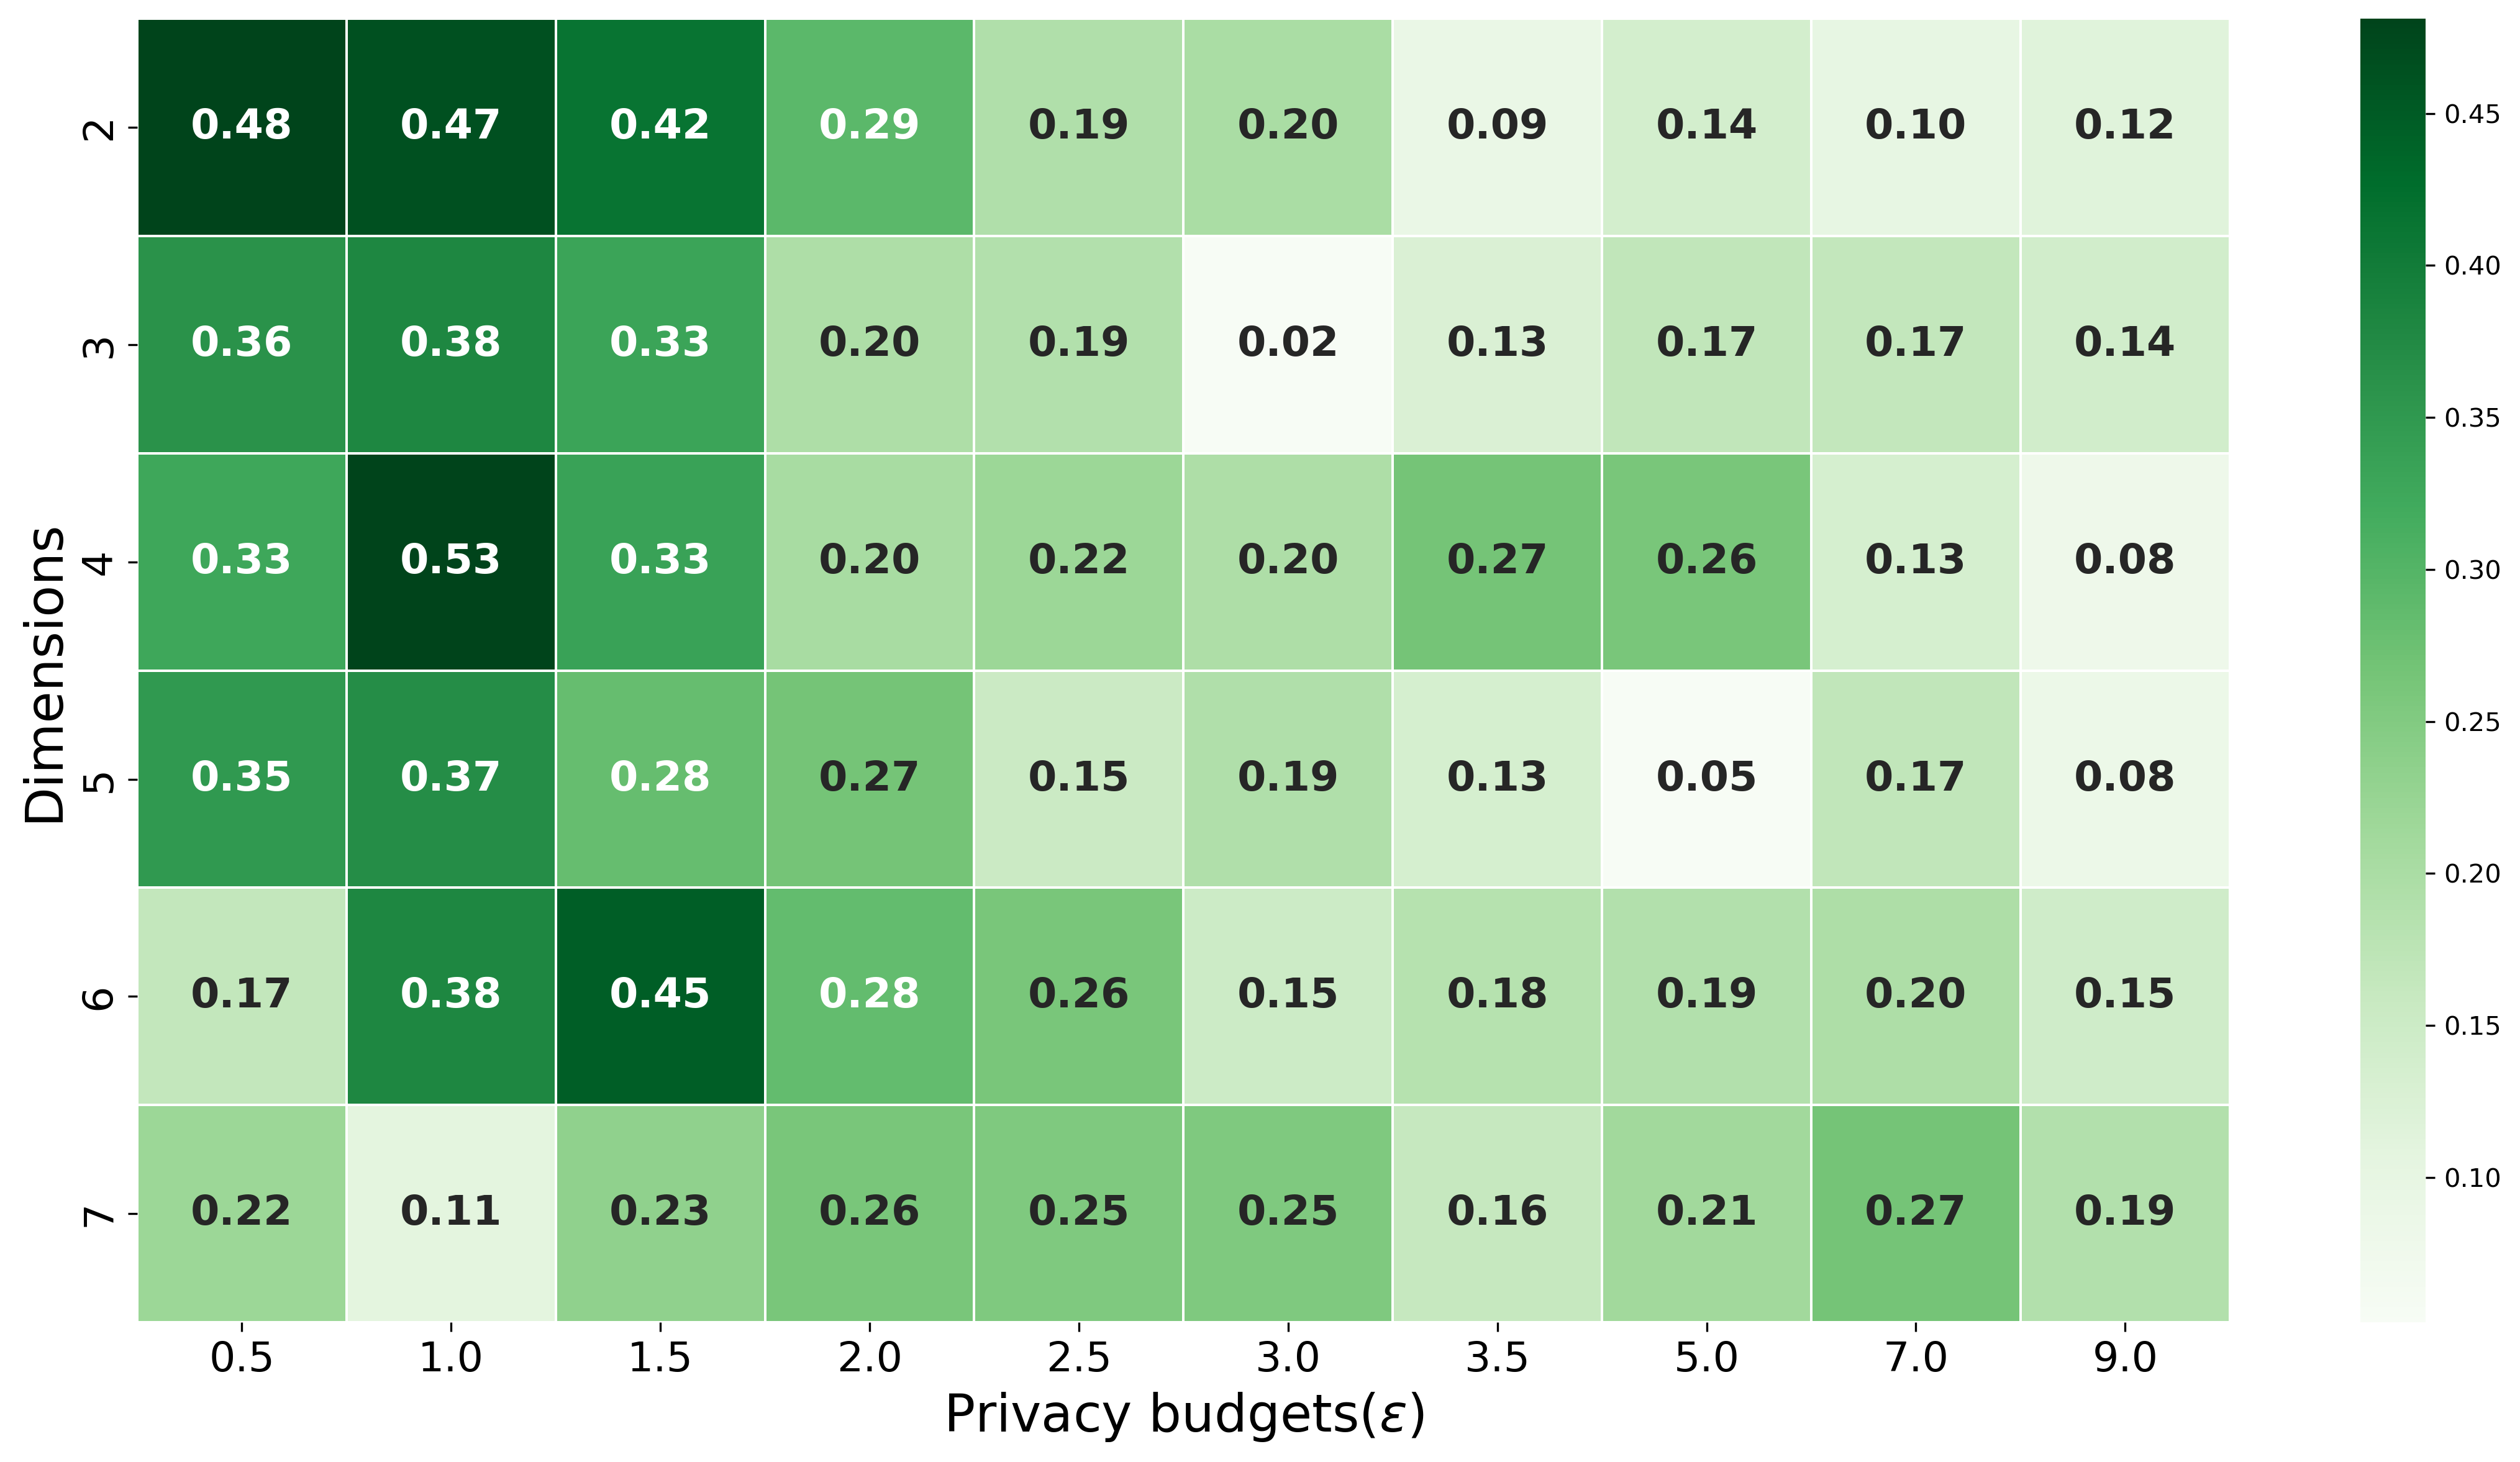
\includegraphics[width=1\textwidth]{Results/nd-laplace/piecewise/seeds-dataset/attack_adv.png}
      \label{fig:privacy_seeds-dataset_adversial_advantage_piecewise}
    \end{subfigure}
  \end{subfigure}
\end{figure}
When comparing the mechanisms, we observe that nD-Laplace has a relatively high score for epsilon values ranging from 0.5 to 2. The dimensions also seem to influence this, as dimensions  7 appears slightly lighter. While, for privacy budgets 7 and 9 the dimensions 6 and 7 are  darker. As the privacy budgets increase, the adversary advantage decreases. This trend is also evident in the Piecewise mechanism. The number of dimensions doesn't have much influence, but it's clear that for epsilons 0.5 to 1.5, the dimensional data has a higher adversary advantage.

We would expect the adversary advantage increasing from left to right, because a higher privacy budget indicates low noise. So, as a consequence the membership advantage should be higher.
To get a clearer picture why this is not happening, we consider the \gls{tpr} for a better illustration of the behaviour (See next page). \newpage
\begin{figure}[H]
    \centering
    \begin{subfigure}[b]{0.75\textwidth}
        \begin{subfigure}[c]{1\textwidth}
            \caption{\textbf{Heatmap TPR for the kD-Laplace mechanism, per privacy budget \& dimension for seeds-dataset.}}
            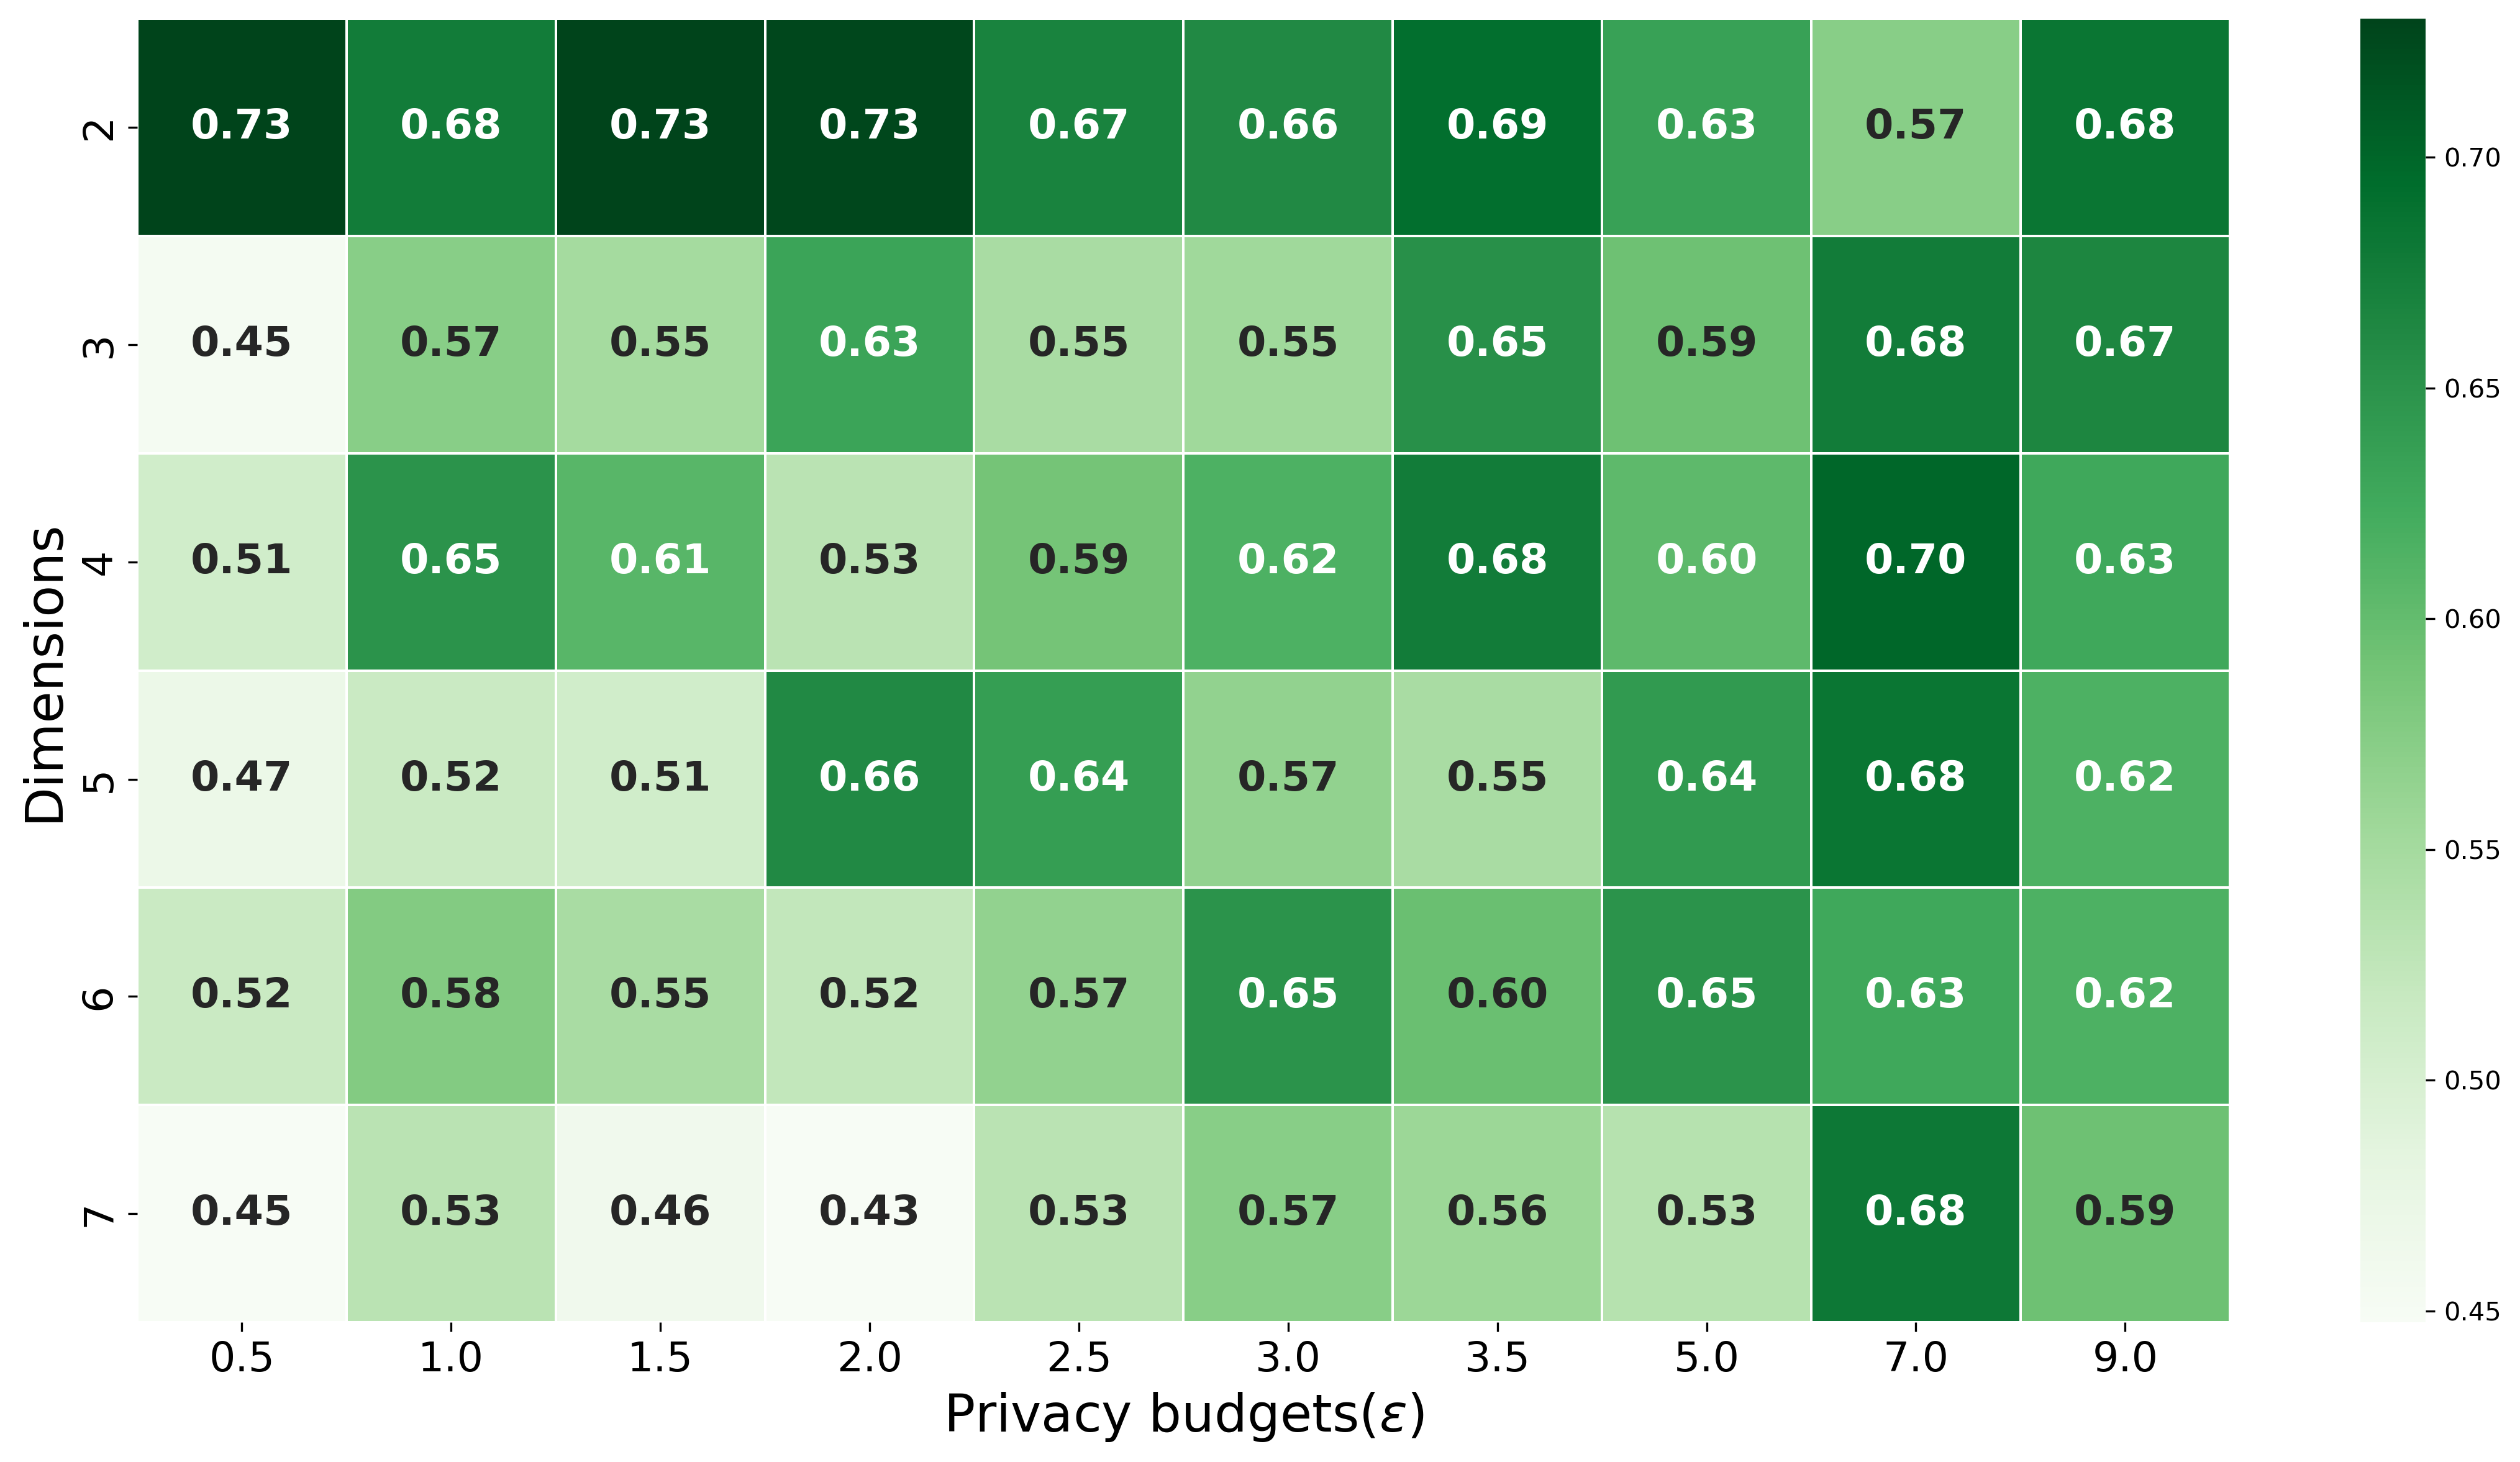
\includegraphics[width=1\textwidth]{Results/nd-laplace/nd-Laplace/seeds-dataset/tpr.png}
            \label{fig:privacy_tpr_seeds-dataset_adversial_advantage_kd-laplace}
        \end{subfigure}
        \vfill % vertical space
        \begin{subfigure}[c]{1\textwidth}
            \caption{\textbf{Heatmap TPR for the Piecewise mechanism, per privacy budget \& dimension for seeds-dataset.}}
            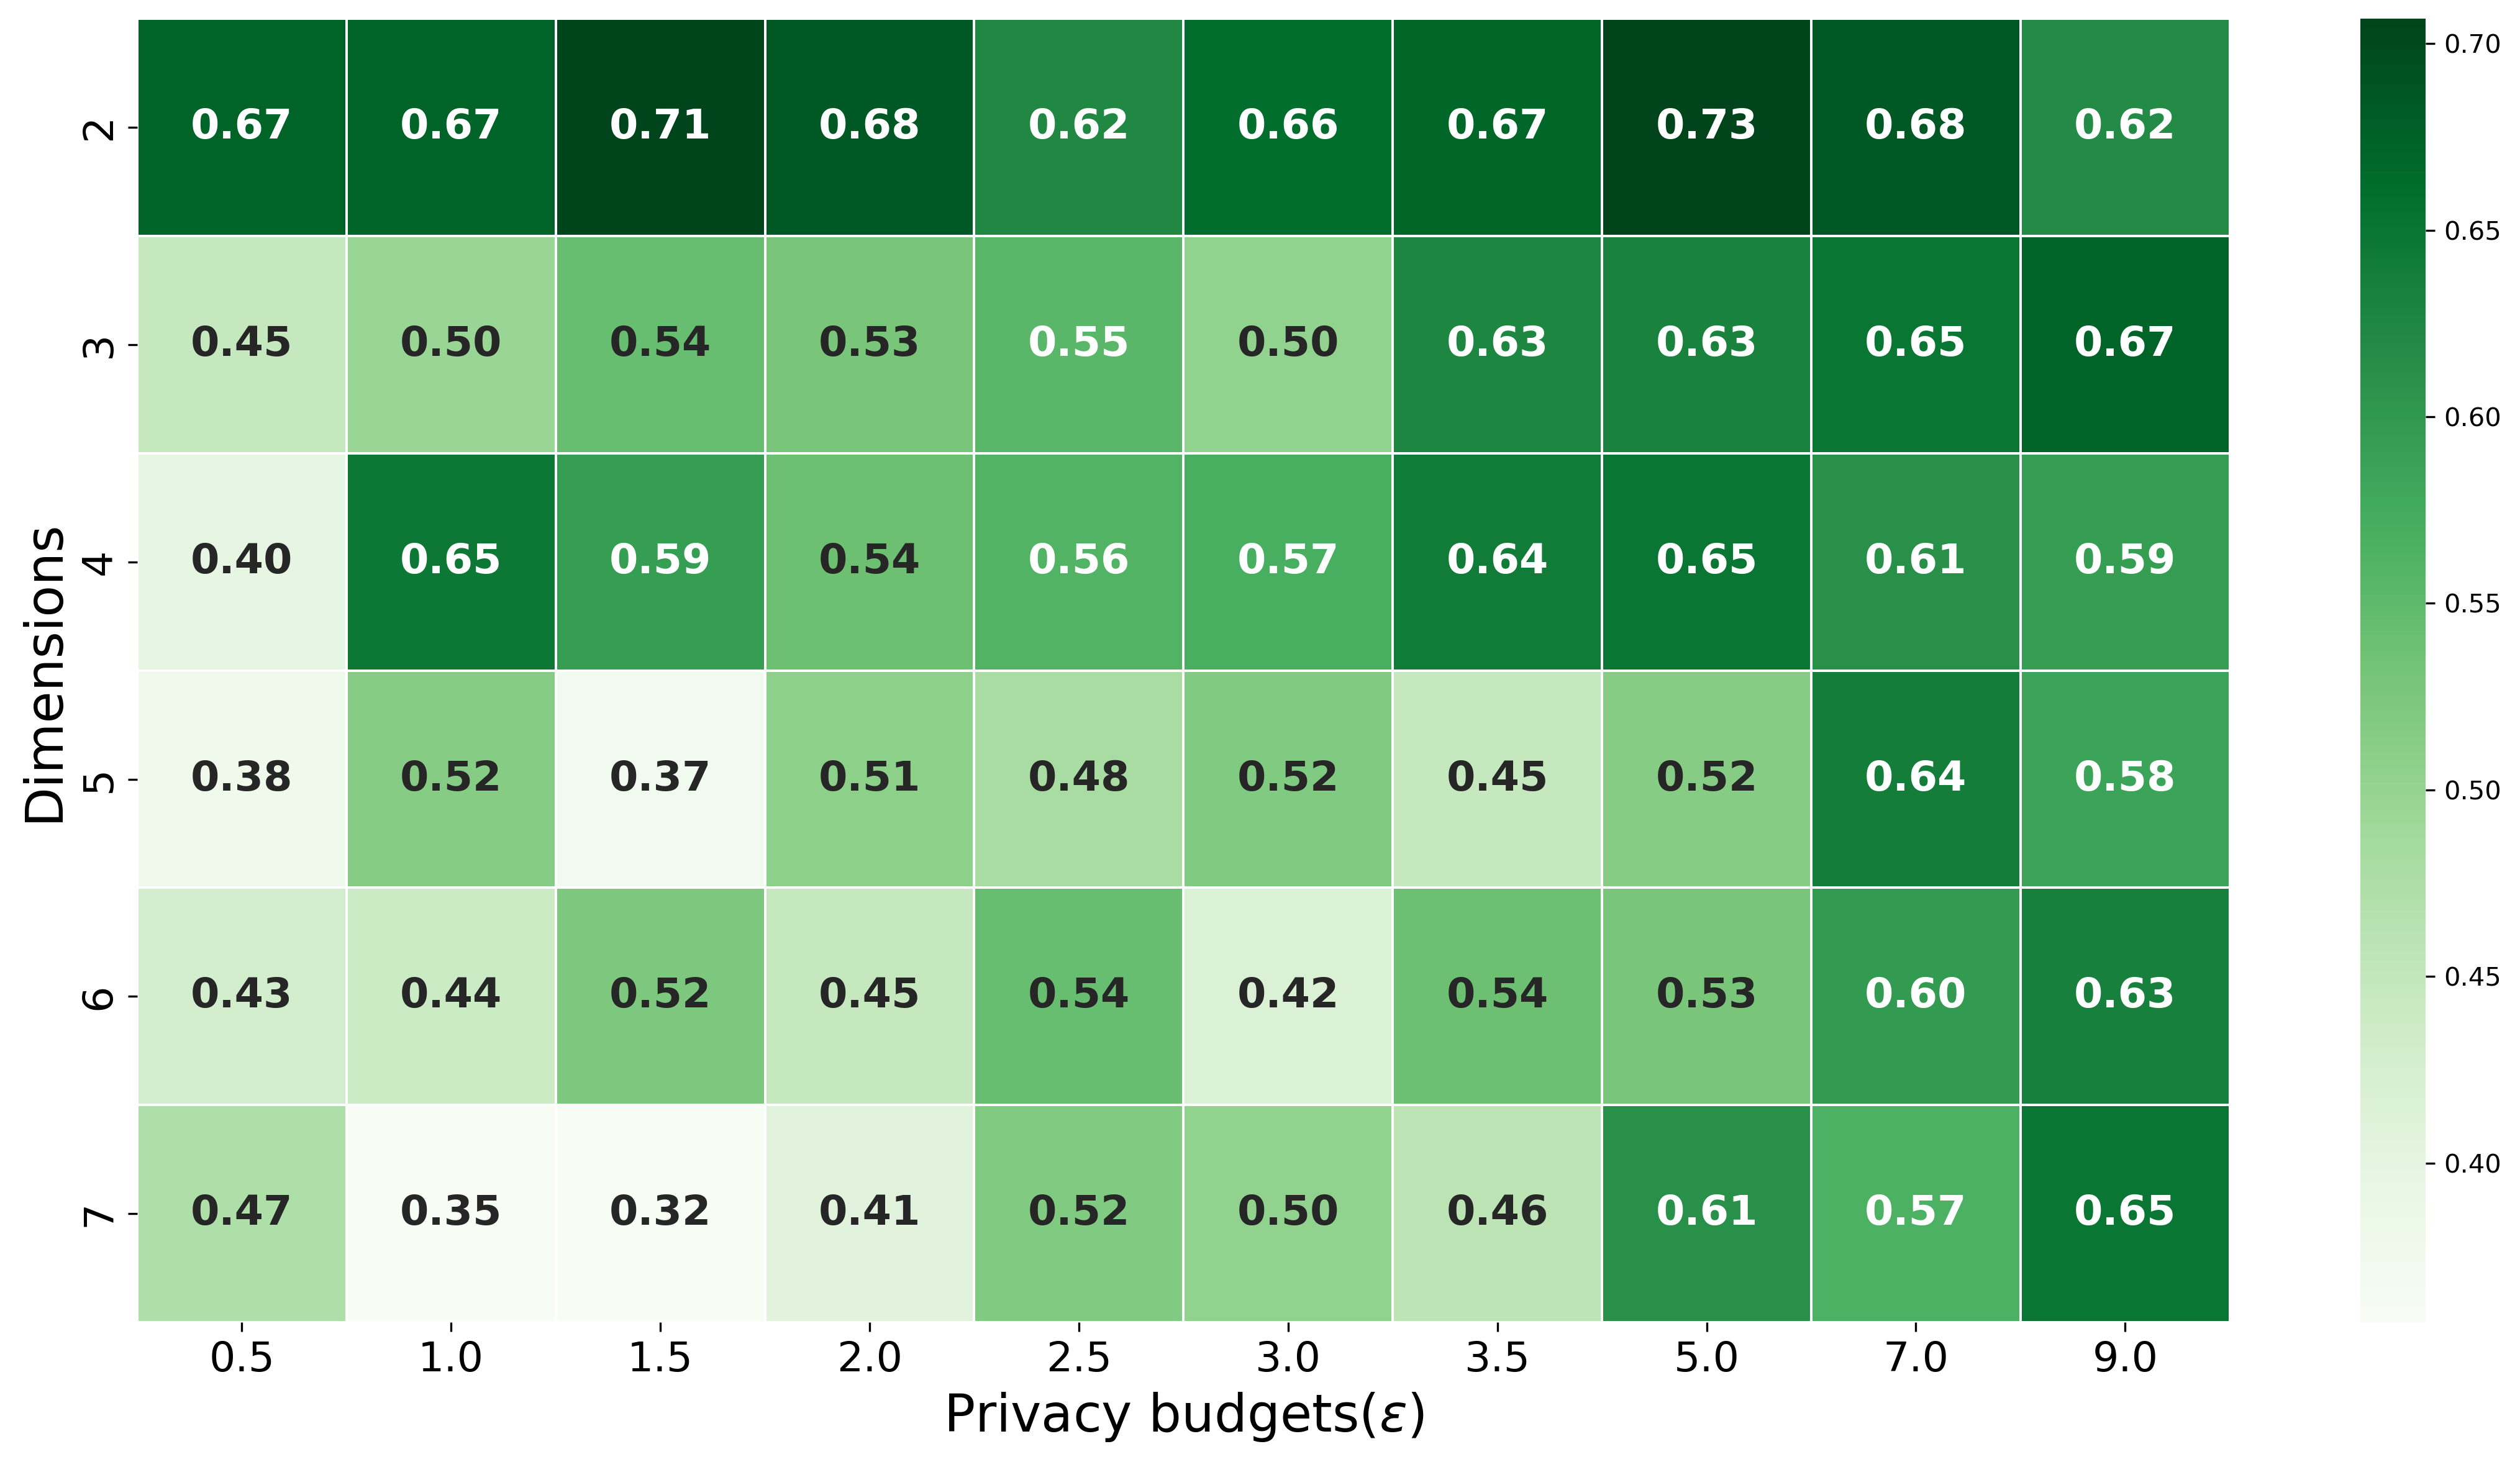
\includegraphics[width=1\textwidth]{Results/nd-laplace/piecewise/seeds-dataset/tpr.png}
            \label{fig:privacy_tpr_seeds-dataset_adversial_advantage_piecewise}
        \end{subfigure}
    \end{subfigure}
\end{figure}
When we examine the plot above, we see a similar pattern. But for Piecewise, the \gls{tpr} for privacy budgets are slightly lower for most of them.
For higher privacy budgets, the \gls{tpr} for both increases to 0.65.
From the \gls{tpr}, it can be inferred that a higher privacy budget indeed leaks more information.
The dimensions have little impact on this, but for both mechanisms, it's observable that 2-dimensions have the highest \gls{tpr}, thereby leaking the most information.
\todo[inline]{Why higher for 2D?}

\newpage
\subsection{Heart dataset}
\begin{figure}[H]
  \centering
  \begin{subfigure}[b]{0.75\textwidth}
    \begin{subfigure}[c]{1\textwidth}
      \caption{\textbf{Heatmap showing adversary advantage for the nD-Laplace mechanism, per privacy budget \& dimension for heart-dataset.}}
      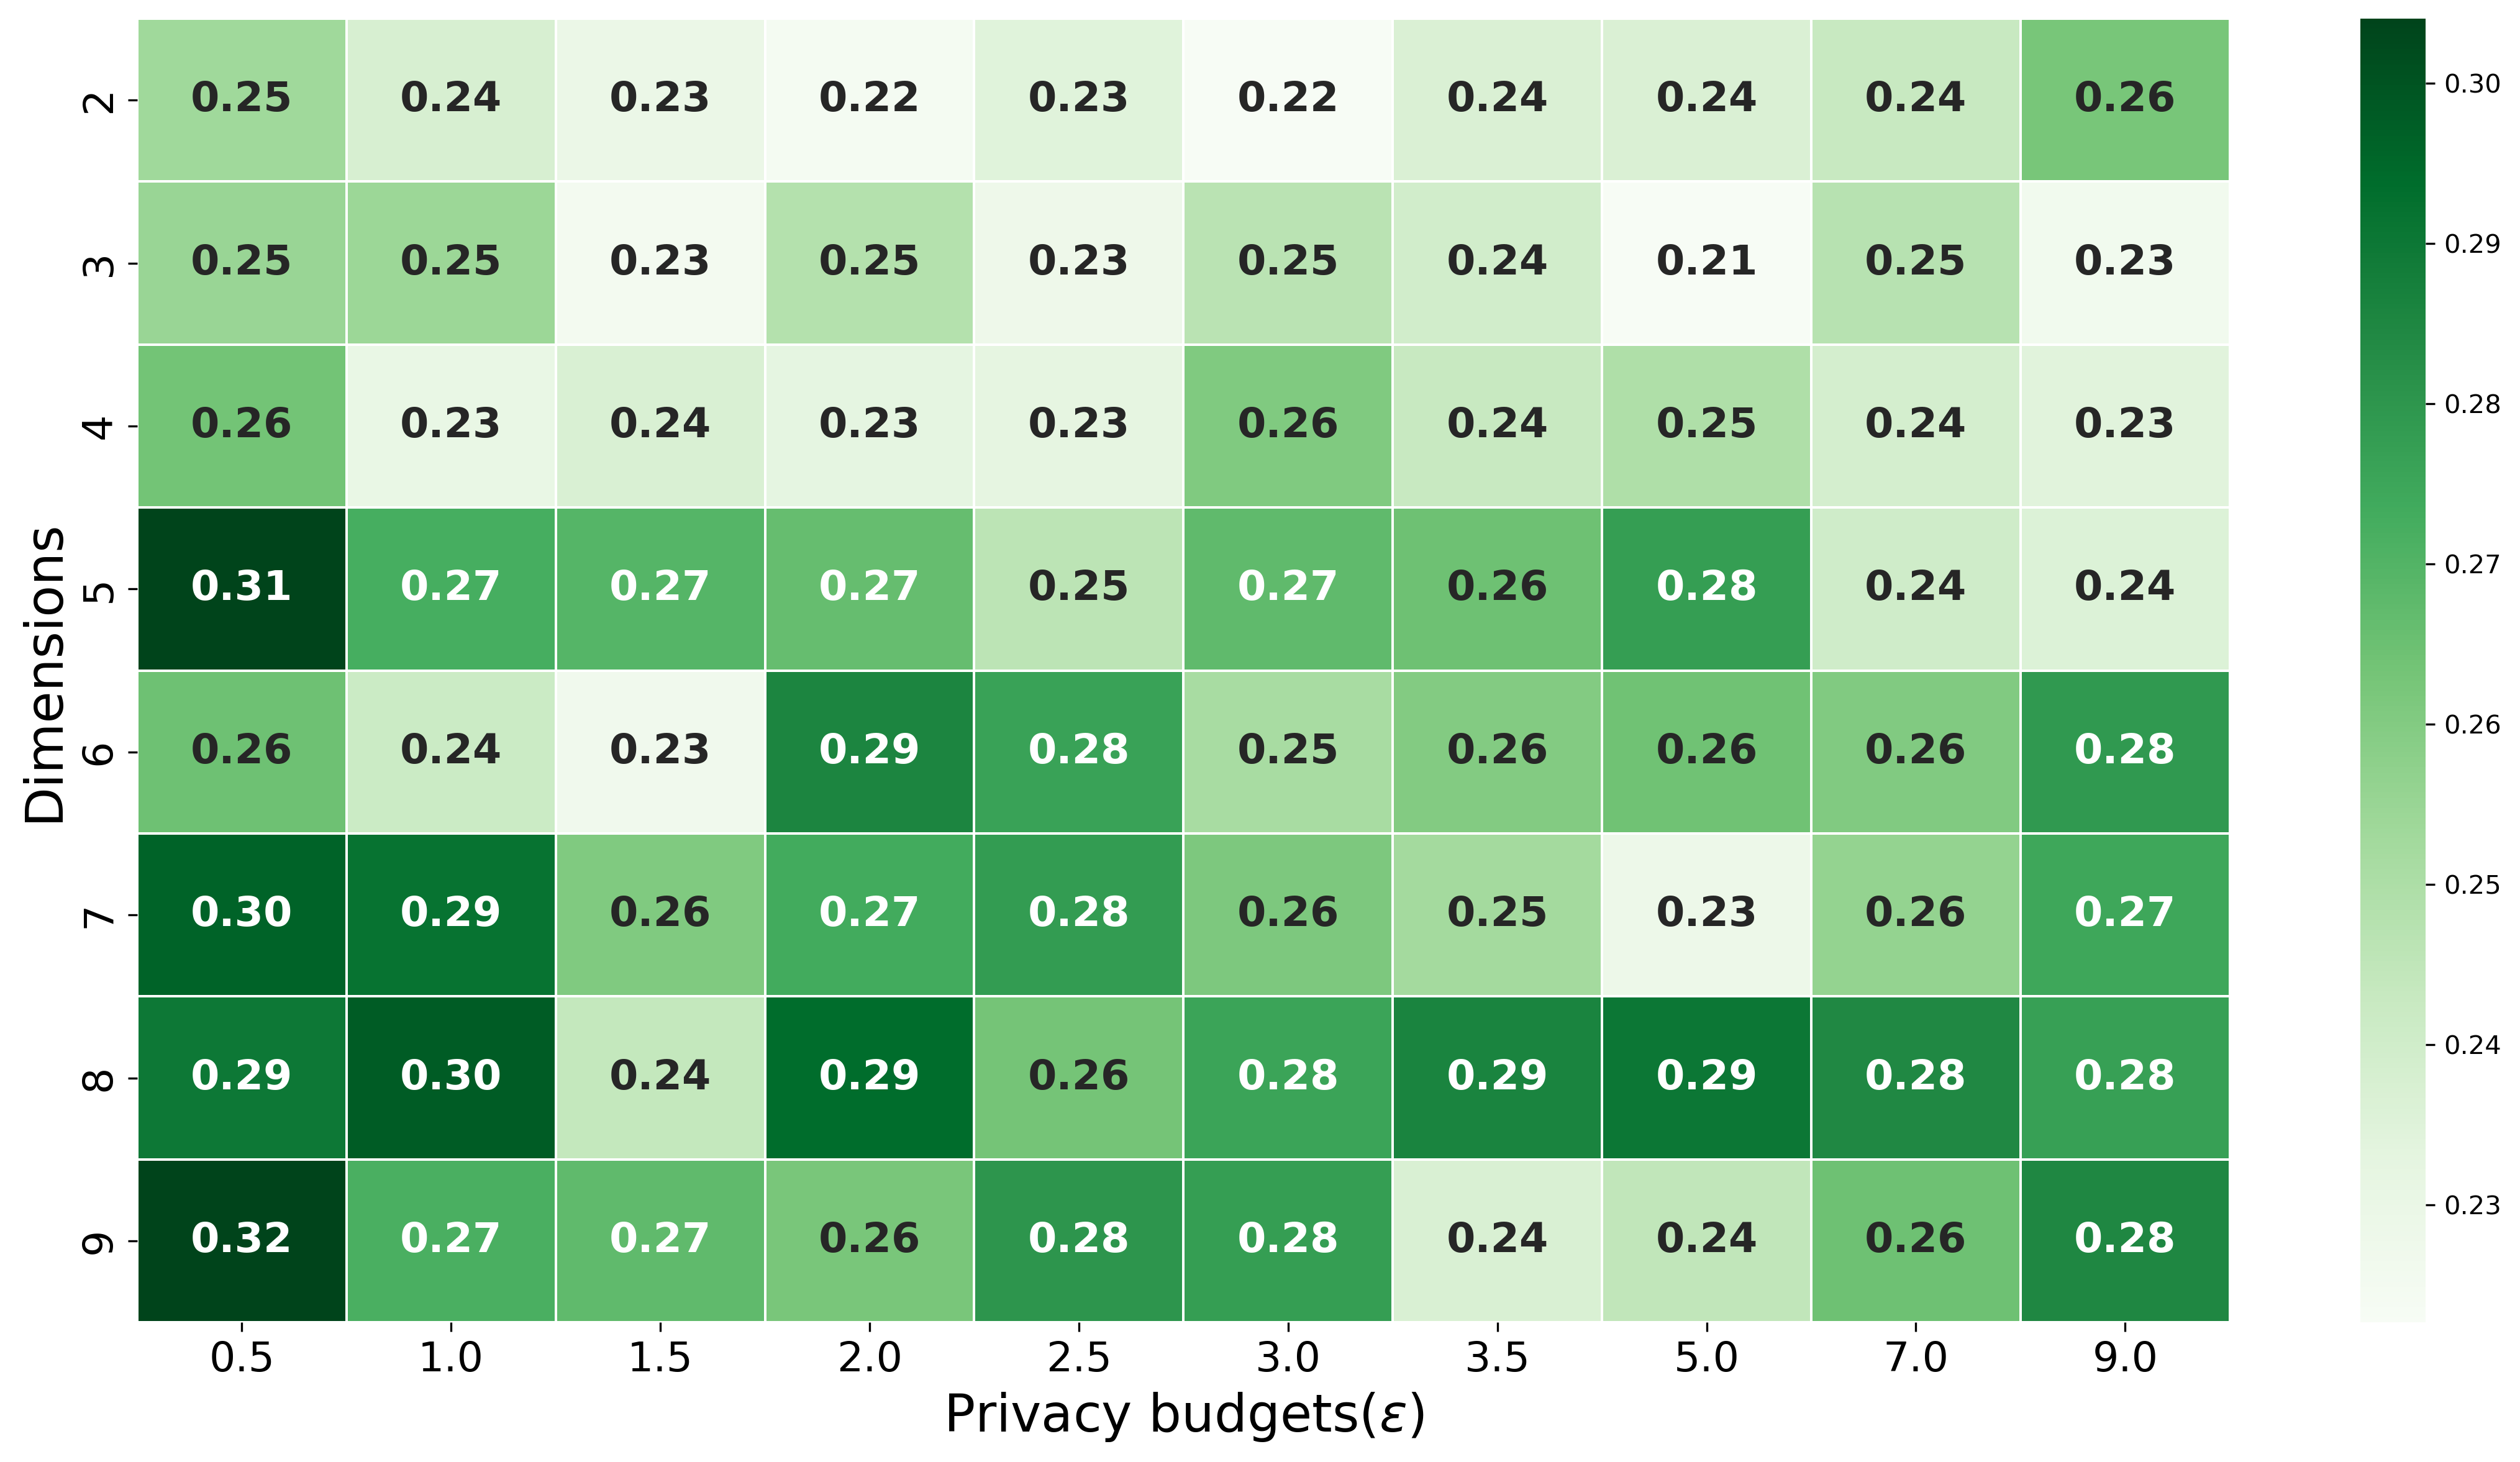
\includegraphics[width=1\textwidth]{Results/nd-laplace/nd-Laplace/heart-dataset/attack_adv.png}
      \label{fig:privacy_heart-dataset_adversial_advantage_kd-laplace}
    \end{subfigure}
    \vfill % vertical space

    \begin{subfigure}[c]{1\textwidth}
      \caption{\textbf{Heatmap showing adversary advantage for the Piecewise mechanism, per privacy budget \& dimension for heart-dataset.}}
      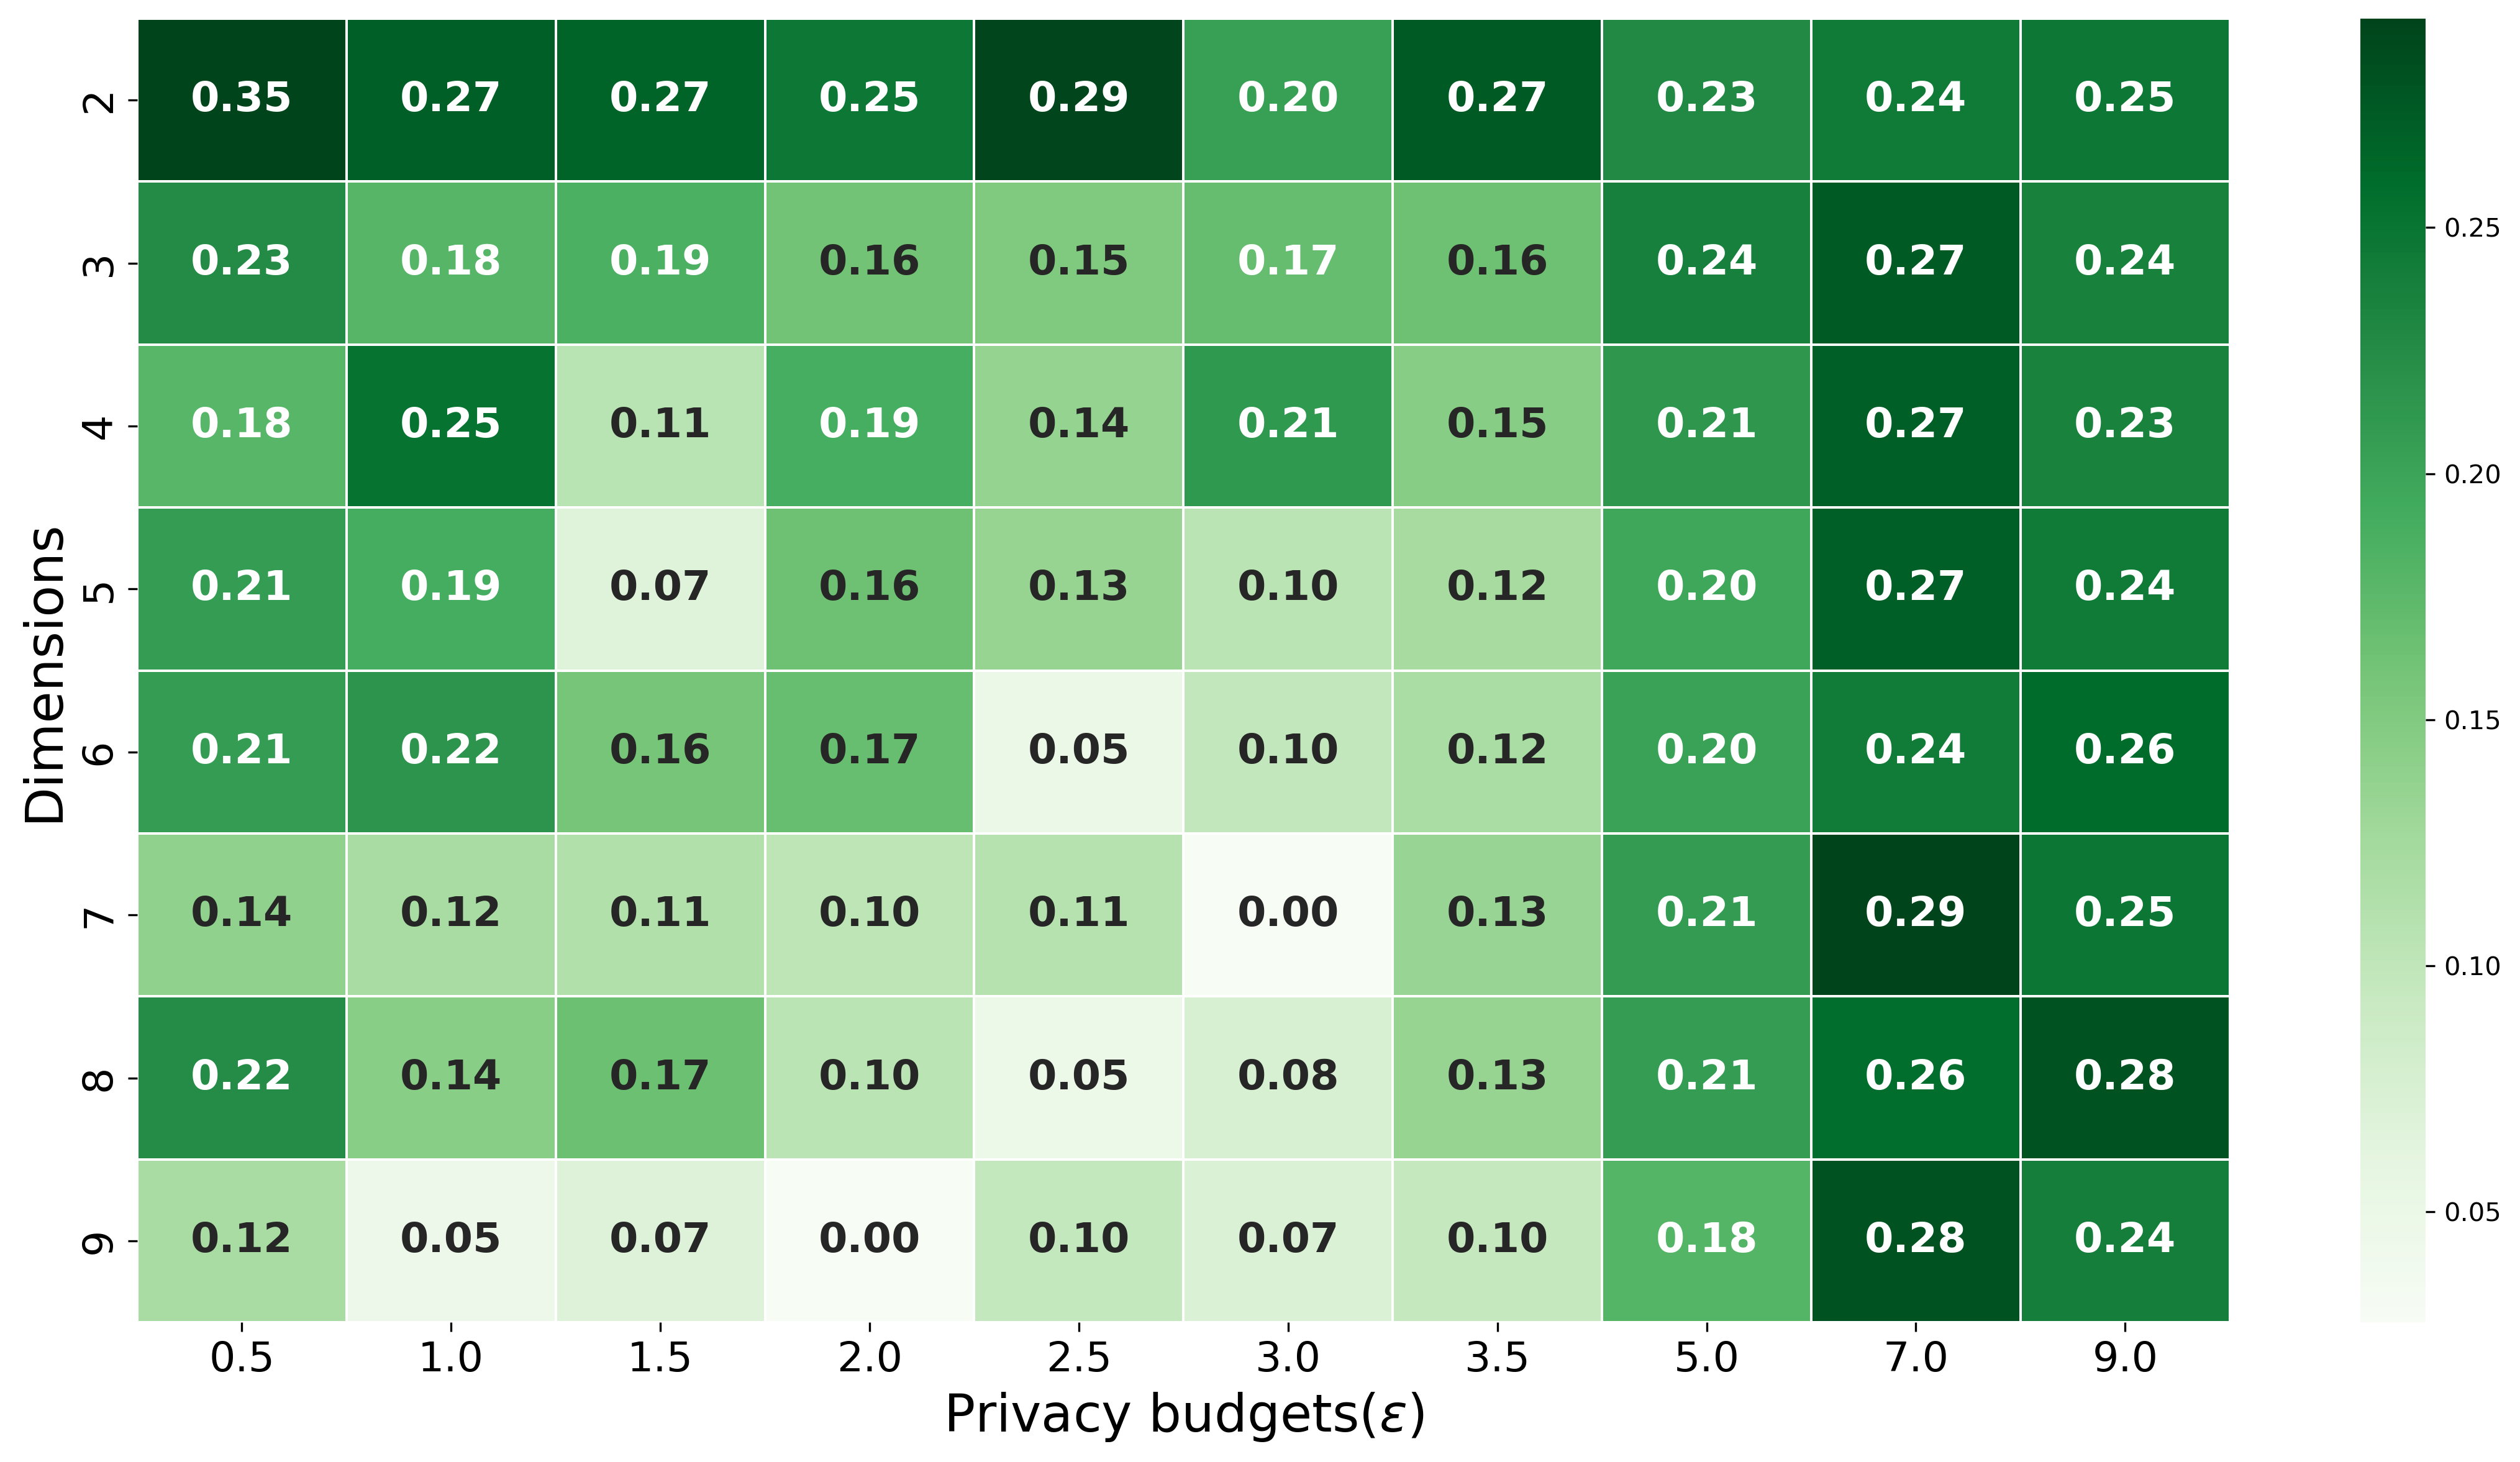
\includegraphics[width=1\textwidth]{Results/nd-laplace/piecewise/heart-dataset/attack_adv.png}
      \label{fig:privacy_heart-dataset_adversial_advantage_piecewise}
    \end{subfigure}
  \end{subfigure}
\end{figure}
For the nD-Laplace mechanism, there's little difference observed between the privacy budgets and dimensions. This is expected, as there's also minimal variation in the \gls{ami} score across different privacy budgets. However, a correlation can be seen between lower dimensions (2 / 3) and the impact of higher privacy budgets. For these dimensions, the adversary advantage is approximately 5 points lower than the other dimensions.
With the Piecewise mechanism, there is a different pattern. For 2-dimensional data, the membership advantage is the highest. When the amount of dimensions increases, the advantage decreases. Higher privacy budgets however seem to have a negative impact, as the advantage increases. This is what we would expect.
Although the adversary advantage in these heatmaps follows a somewhat more logical progression for Piecewise (increasing from left to right), it still shows some weird results for nD-Laplace. Therefore we will analyze the \gls{tpr} on the following page. 
\newpage
\begin{figure}[H]
    \centering
    \begin{subfigure}[b]{0.75\textwidth}
        \begin{subfigure}[c]{1\textwidth}
            \caption{\textbf{Heatmap TPR for the kD-Laplace mechanism, per privacy budget \& dimension for heart-dataset.}}
            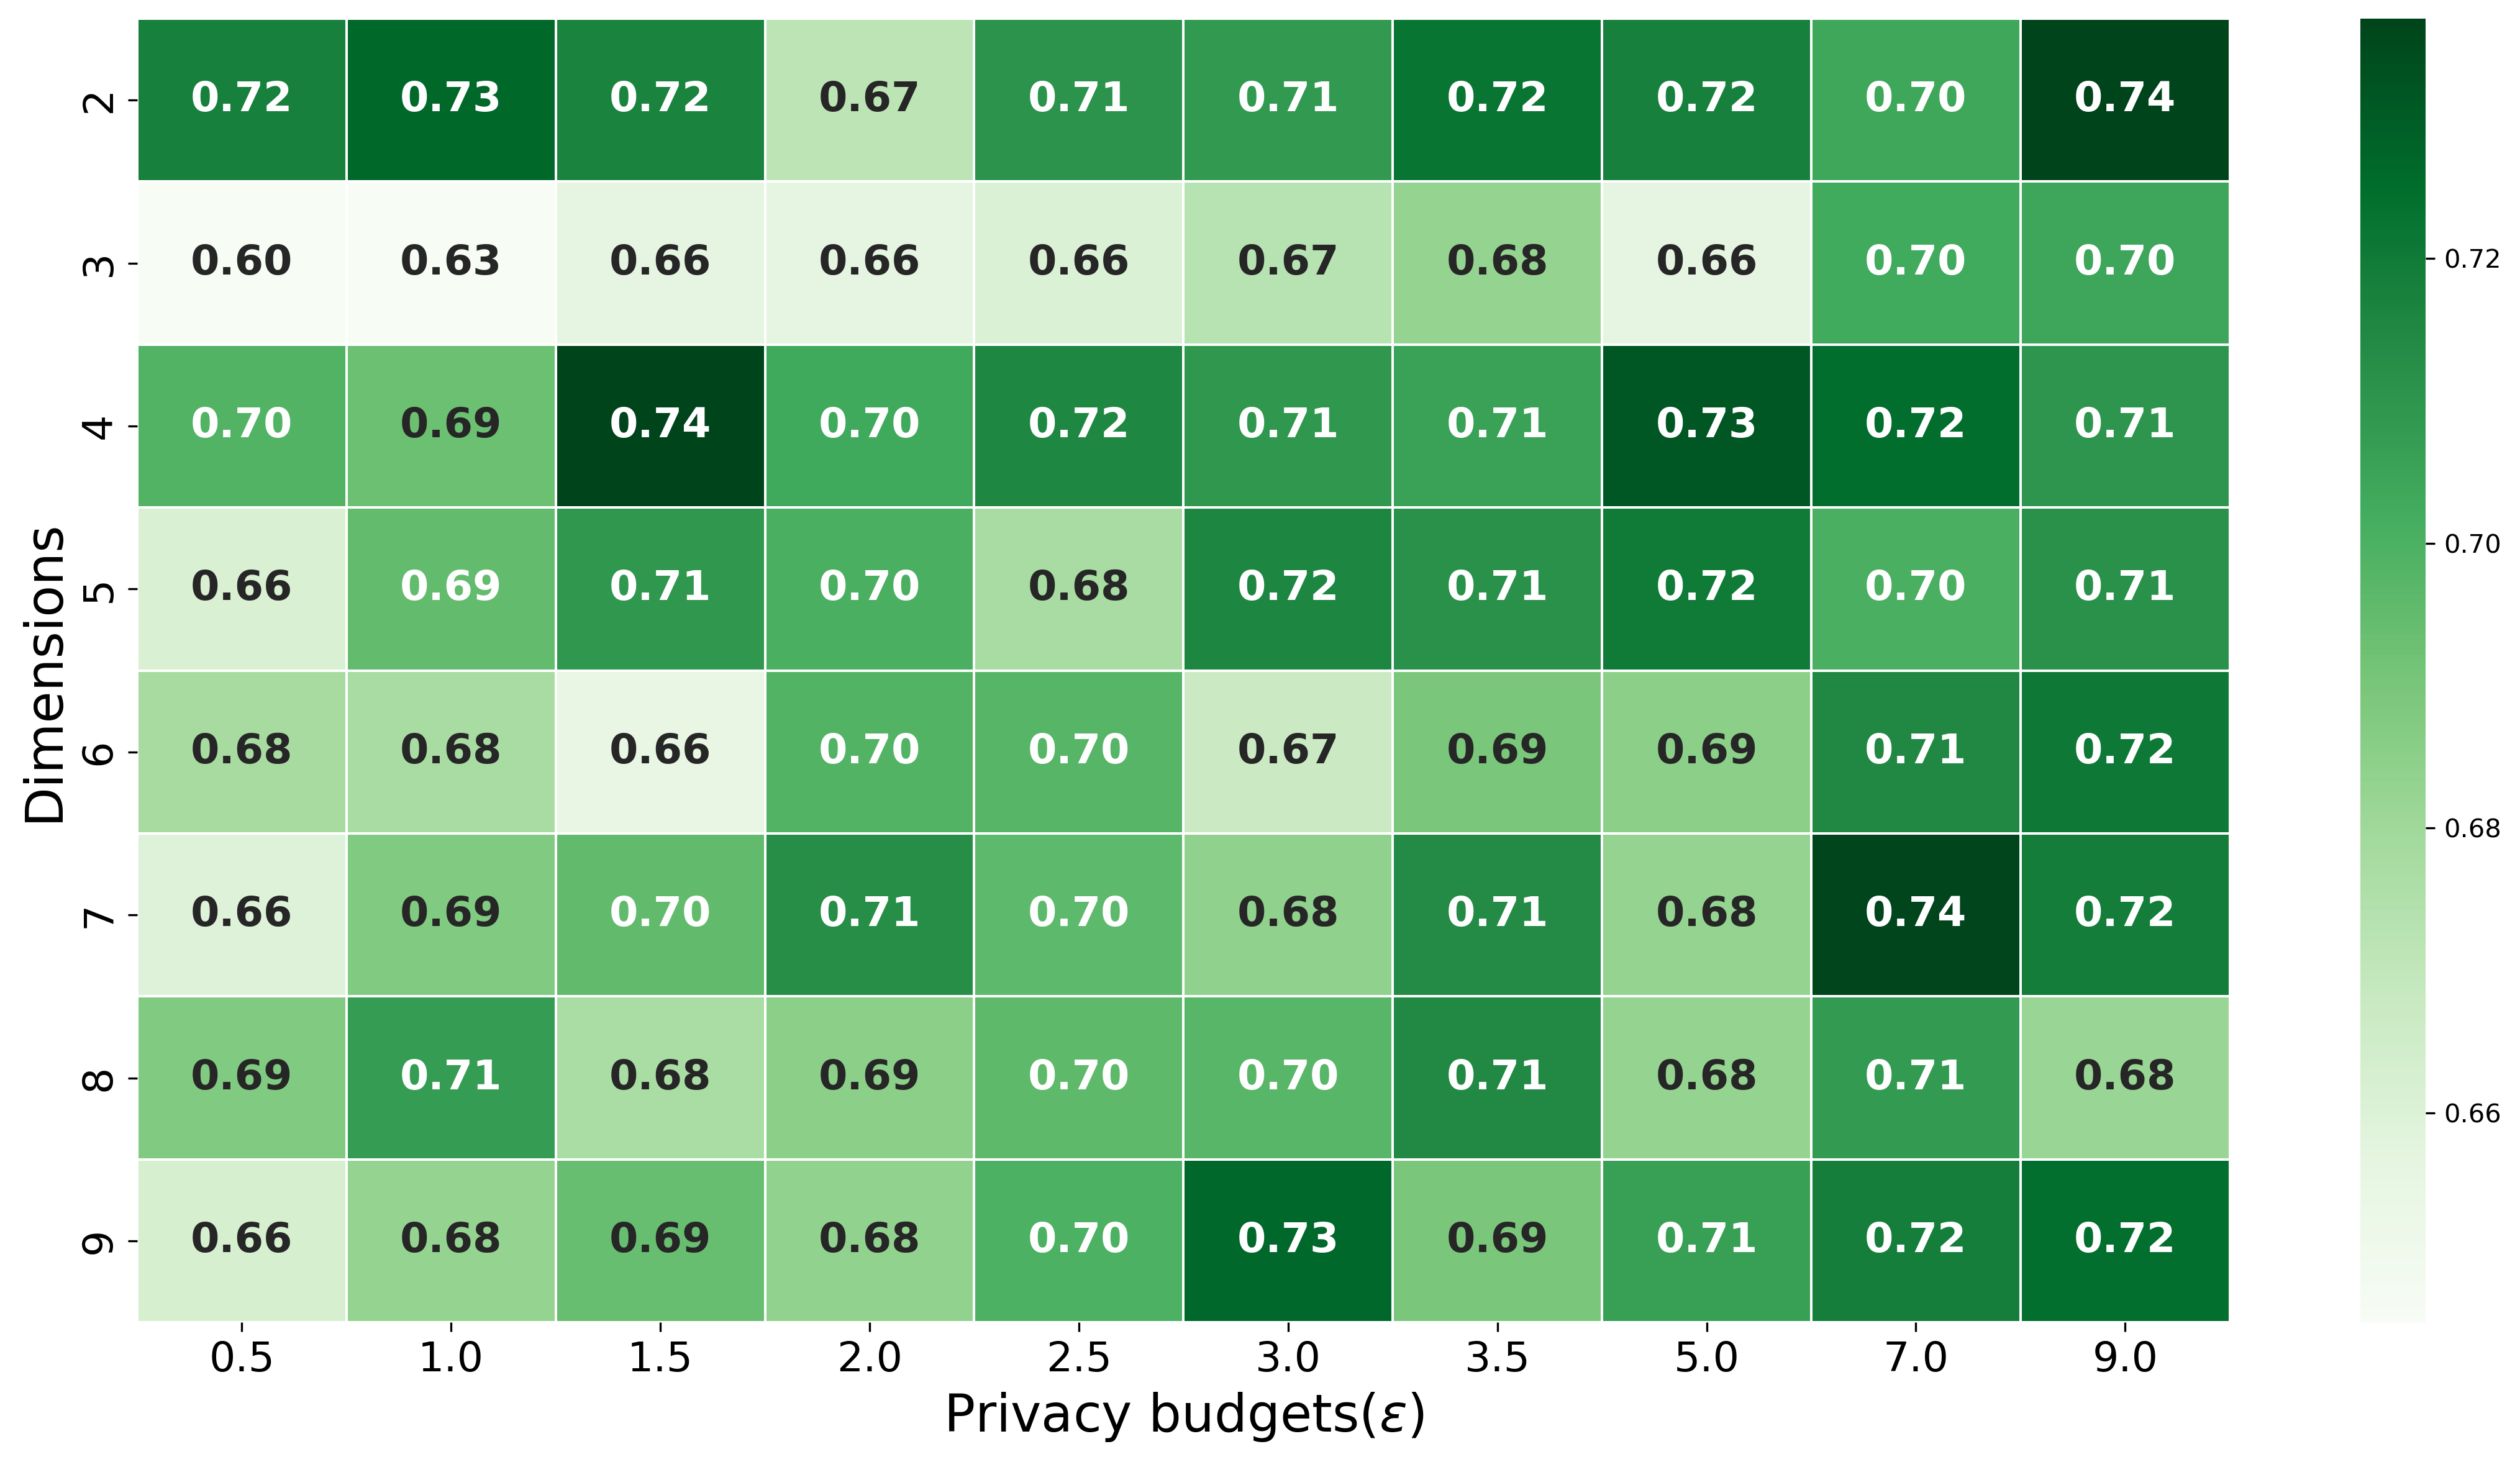
\includegraphics[width=1\textwidth]{Results/nd-laplace/nd-Laplace/heart-dataset/tpr.png}
            \label{fig:privacy_tpr_heart-dataset_adversial_advantage_kd-laplace}
        \end{subfigure}
        \vfill % vertical space

        \begin{subfigure}[c]{1\textwidth}
            \caption{\textbf{Heatmap TPR for the Piecewise mechanism, per privacy budget \& dimension for heart-dataset.}}
            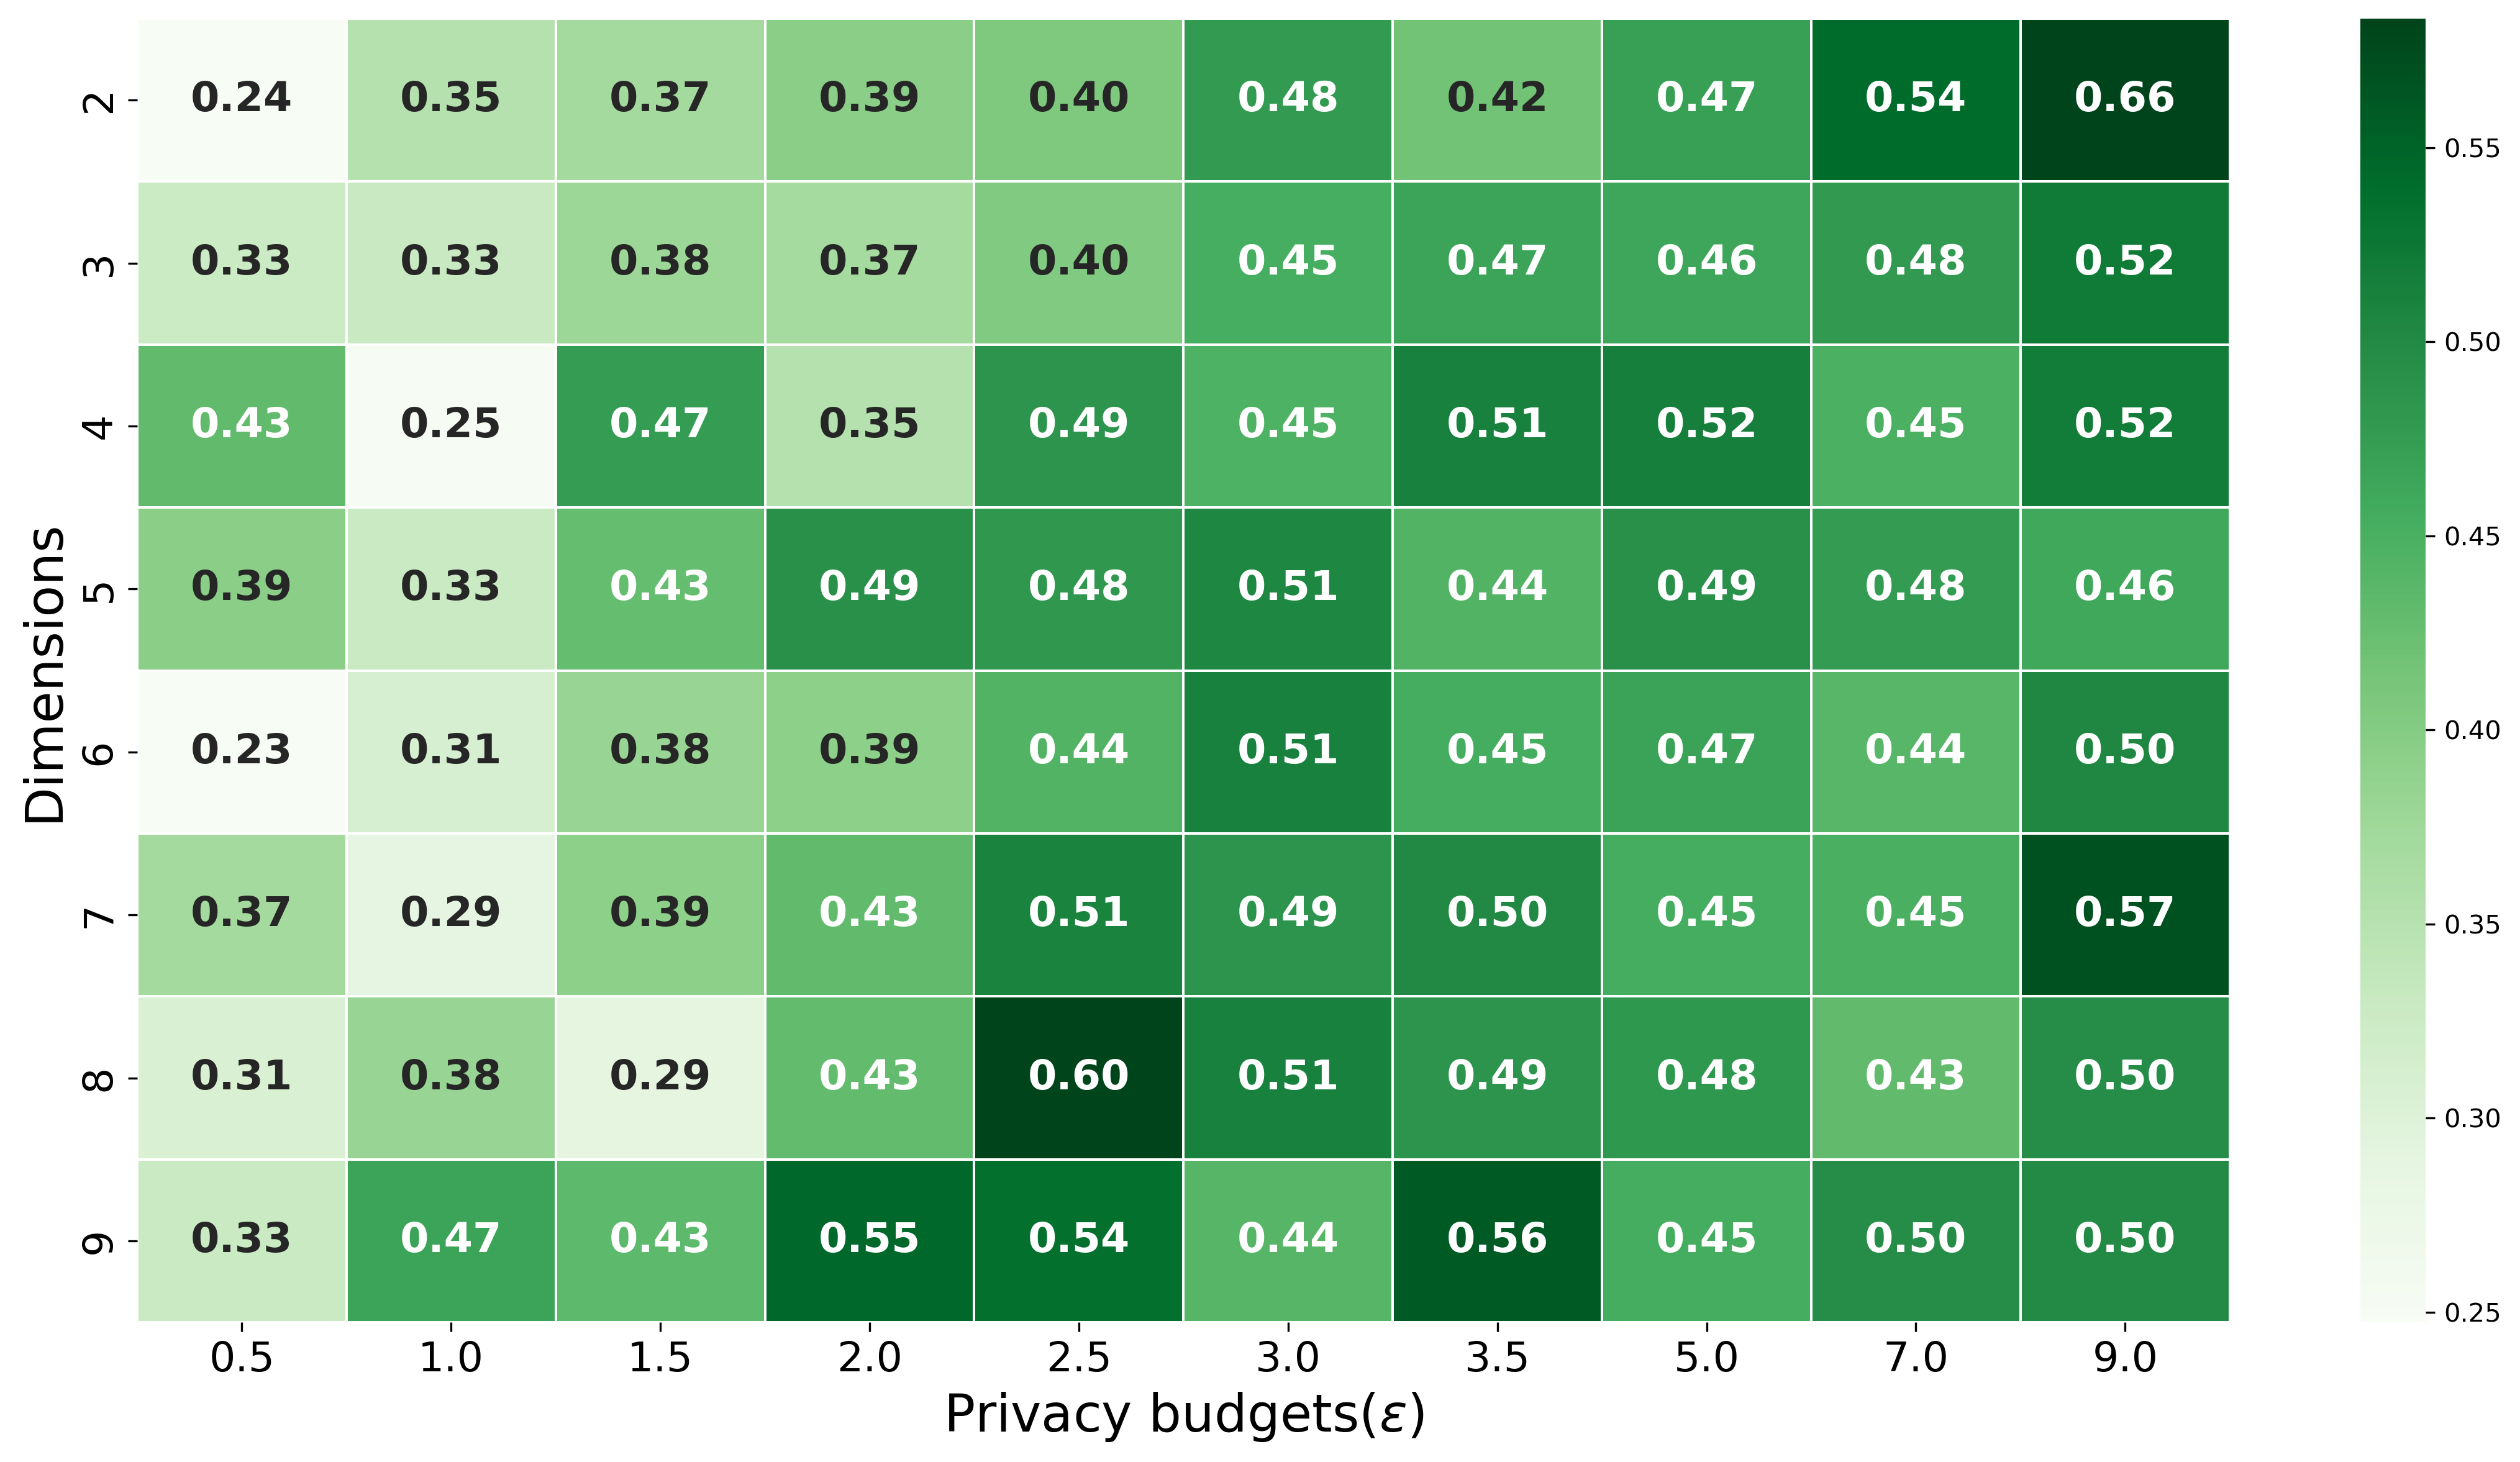
\includegraphics[width=1\textwidth]{Results/nd-laplace/piecewise/heart-dataset/tpr.png}
            \label{fig:privacy_tpr_heart-dataset_adversial_advantage_piecewise}
        \end{subfigure}
    \end{subfigure}
\end{figure}
For the Piecewise mechanism, the results are clear and follow a similar pattern that we also saw with the membership advantage on the previous page.
With the nD-Laplace mechanism, the results are quite varied. We see a slight influence of the privacy budget (0.5 is slightly lower compared to the rest), but overall, no major changes are noticeable.
What stands out is the lower score (approximately 0.10 \gls{tpr}) for 3-dimensions compared to the rest.
\todo[inline]{Why only 3-dimensions?}

\newpage

\subsection{Circle dataset}
\begin{figure}[H]
  \centering
  \begin{subfigure}[b]{0.85\textwidth}
    \begin{subfigure}[c]{1\textwidth}
      \caption{\textbf{Heatmap showing adversary advantage for the kD-Laplace mechanism, per privacy budget \& dimension for circle-dataset.}}
      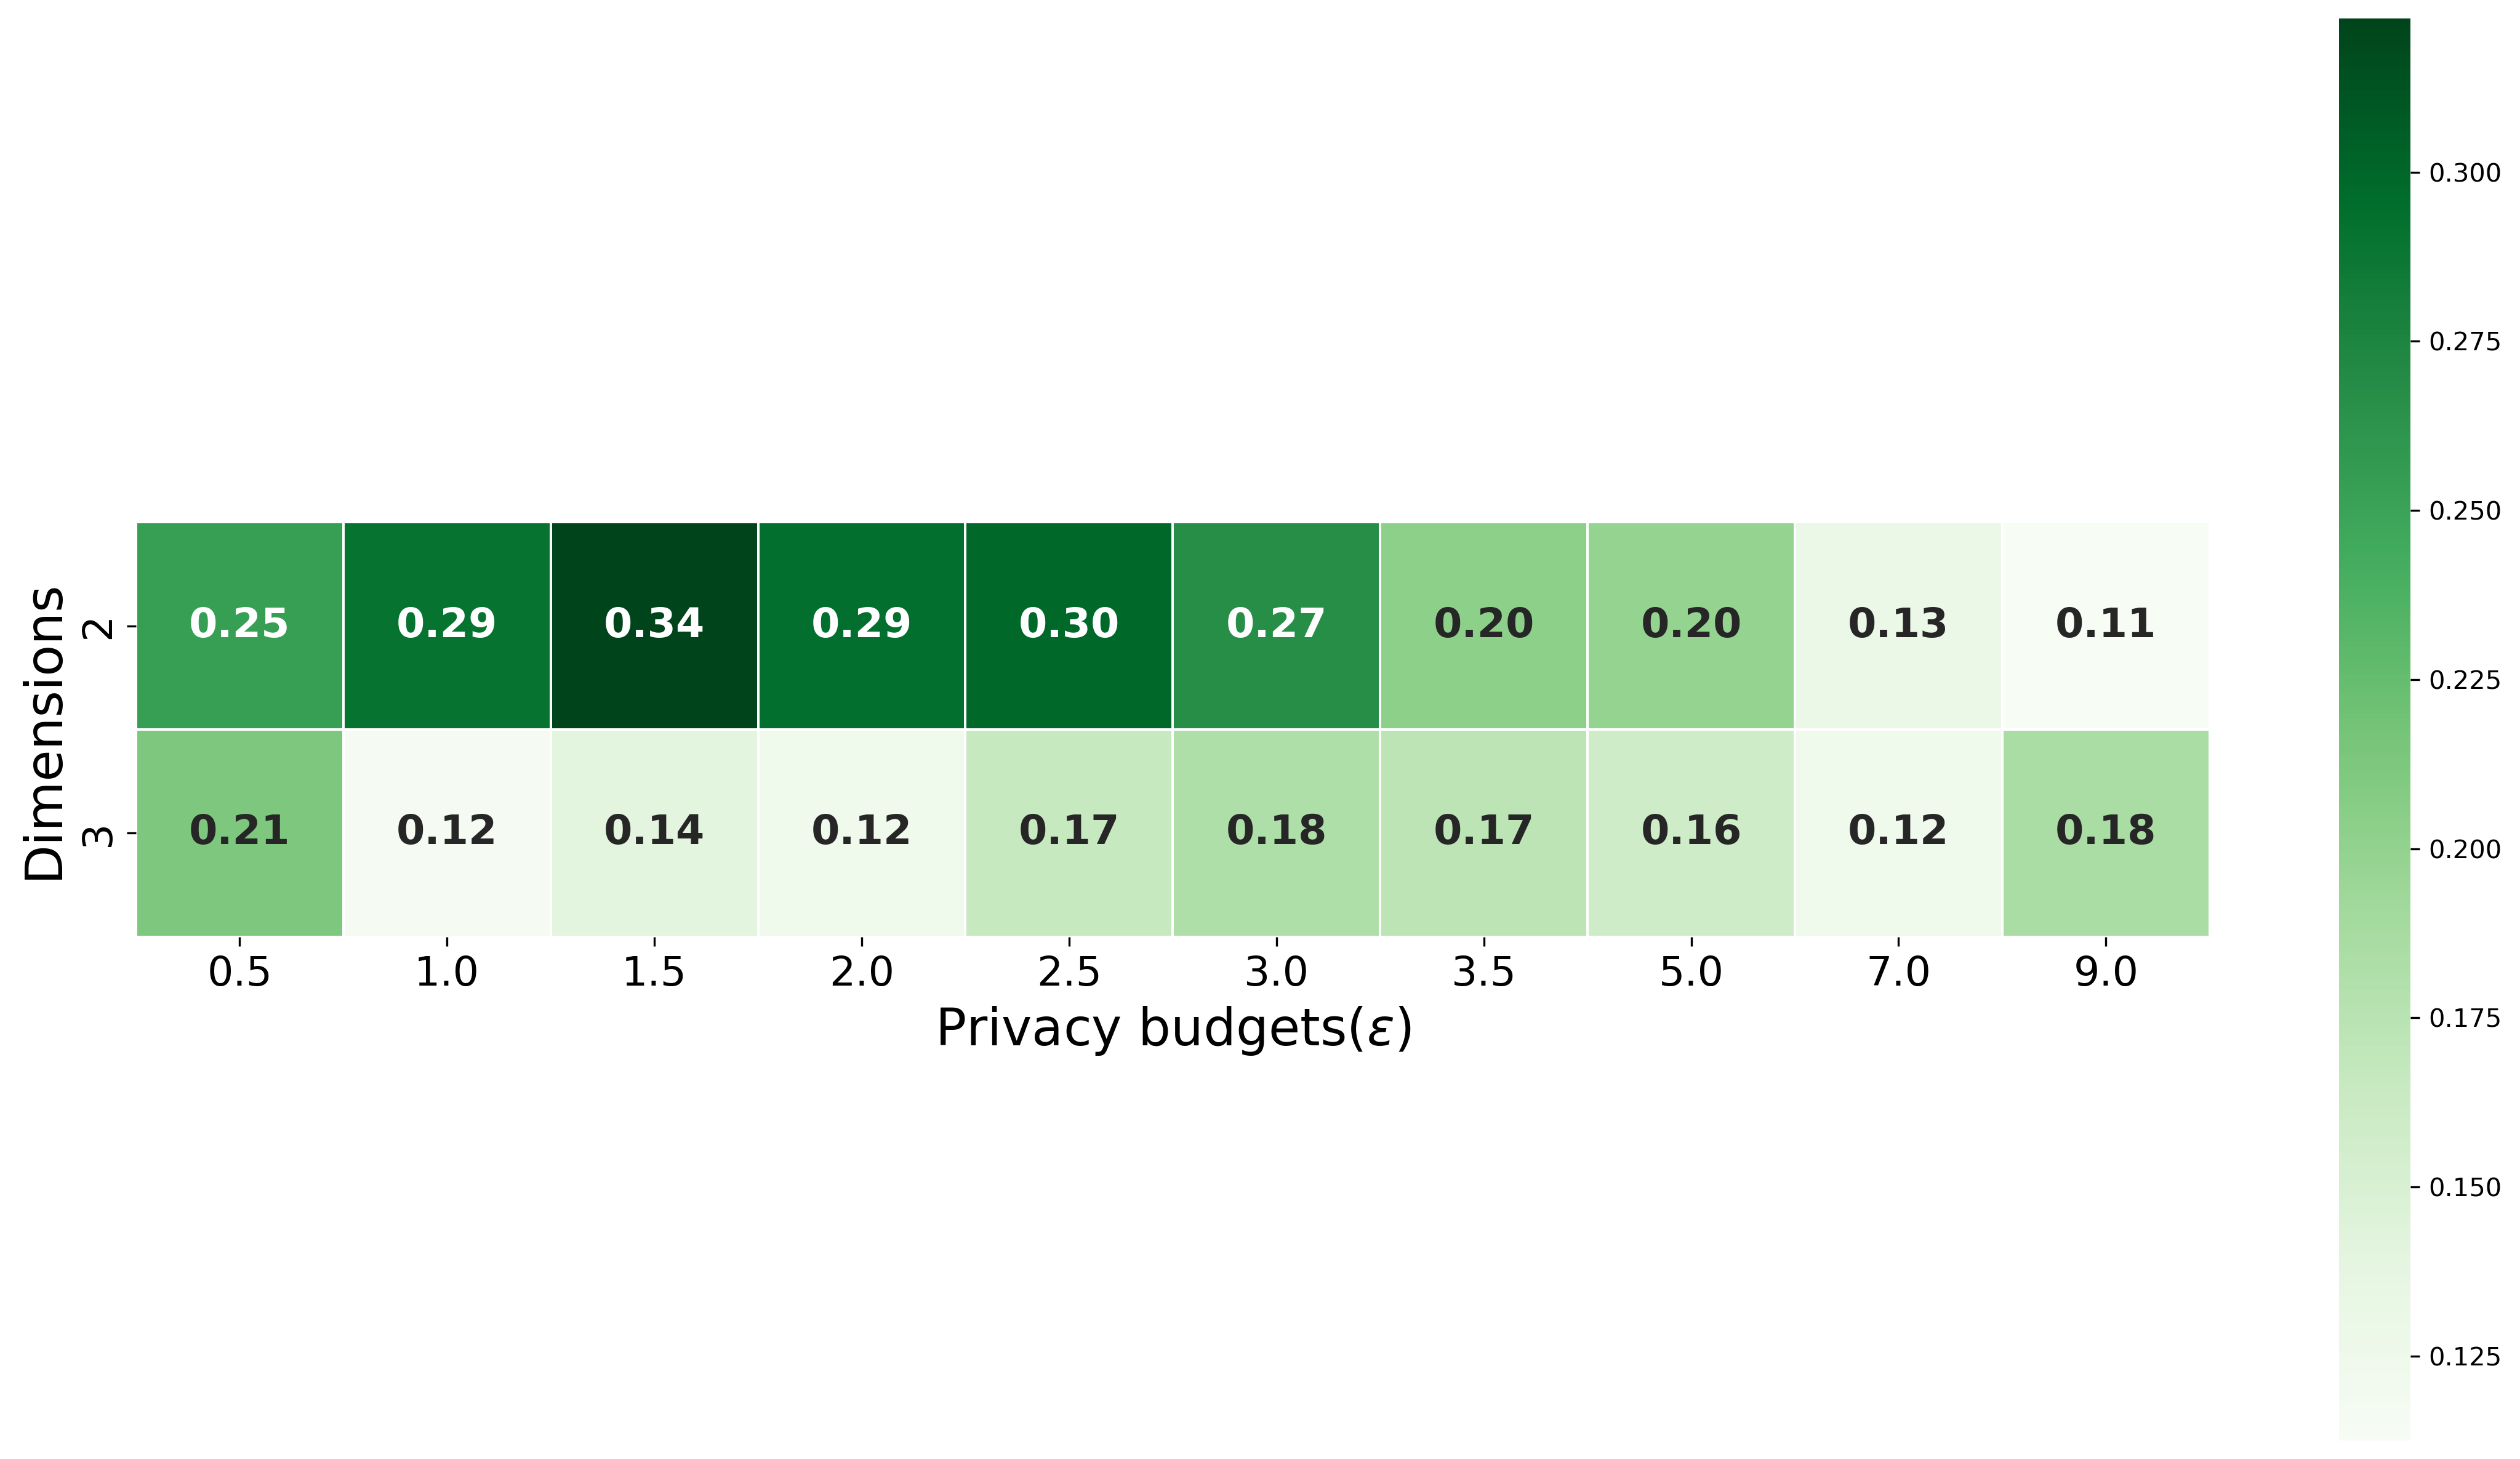
\includegraphics[width=1\textwidth]{Results/nd-laplace/nd-Laplace/circle-dataset/attack_adv.png}
      \label{fig:privacy_circle-dataset_adversial_advantage_kd-laplace}
    \end{subfigure}
    \vfill % vertical space

    \begin{subfigure}[c]{1\textwidth}
      \caption{\textbf{Heatmap showing adversary advantage for the Piecewise mechanism, per privacy budget \& dimension for seeds-dataset.}}
      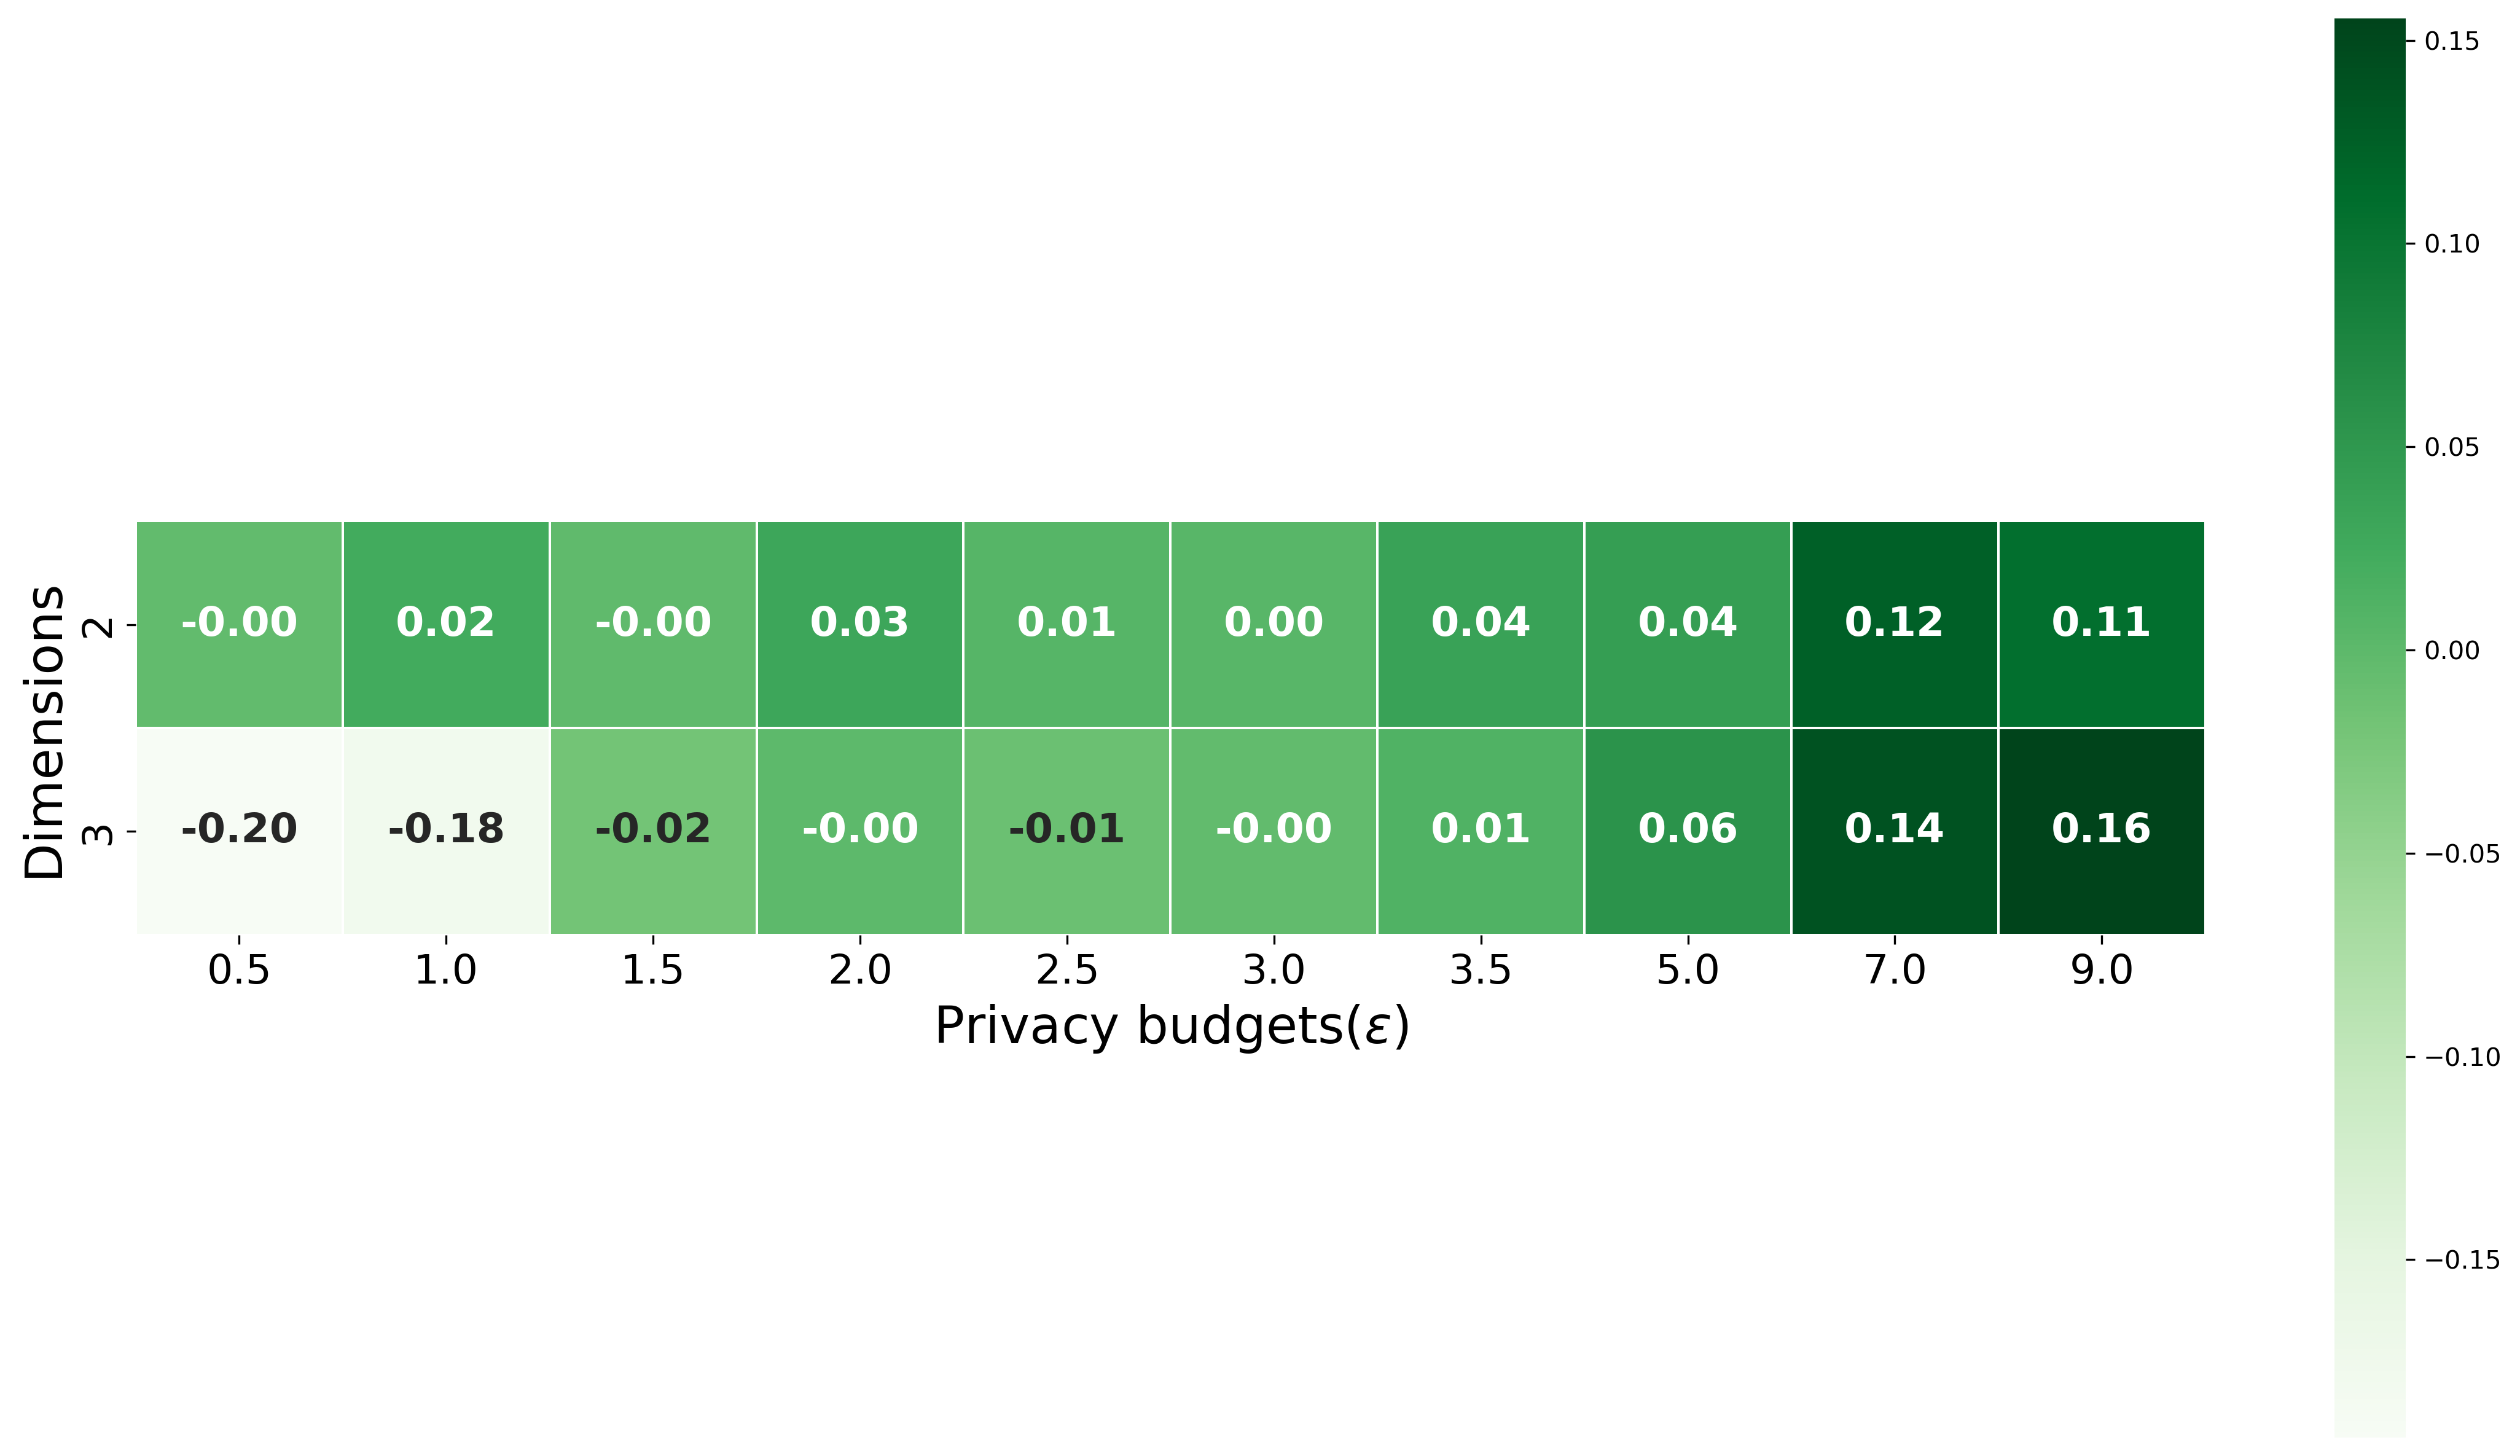
\includegraphics[width=1\textwidth]{Results/nd-laplace/piecewise/circle-dataset/attack_adv.png}
      \label{fig:privacy_circle-dataset_adversial_advantage_piecewise}
    \end{subfigure}
  \end{subfigure}
\end{figure}
For the nD-Laplace mechanism, a pattern is visible that we have also seen in the other plots. The 2-dimensional data is relatively high compared to the other dimensions, and with a higher dimension, the membership advantage is actually lower instead of higher.
The pattern of the Piecewise mechanism is mostly the same. However, on average, the membership advantage is slightly higher.
It's notable that for 2 and 3 dimensions, the value is very low for epsilon 3 and 2, respectively.
On the next page, we will also analyze the \gls{tpr} to get an underlying view of the results.

\newpage
\begin{figure}[H]
    \centering
    \begin{subfigure}[b]{0.9\textwidth}
        \begin{subfigure}[c]{1\textwidth}
            \caption{\textbf{Heatmap TPR for the nD-Laplace mechanism, per privacy budget \& dimension for Circle-dataset.}}
            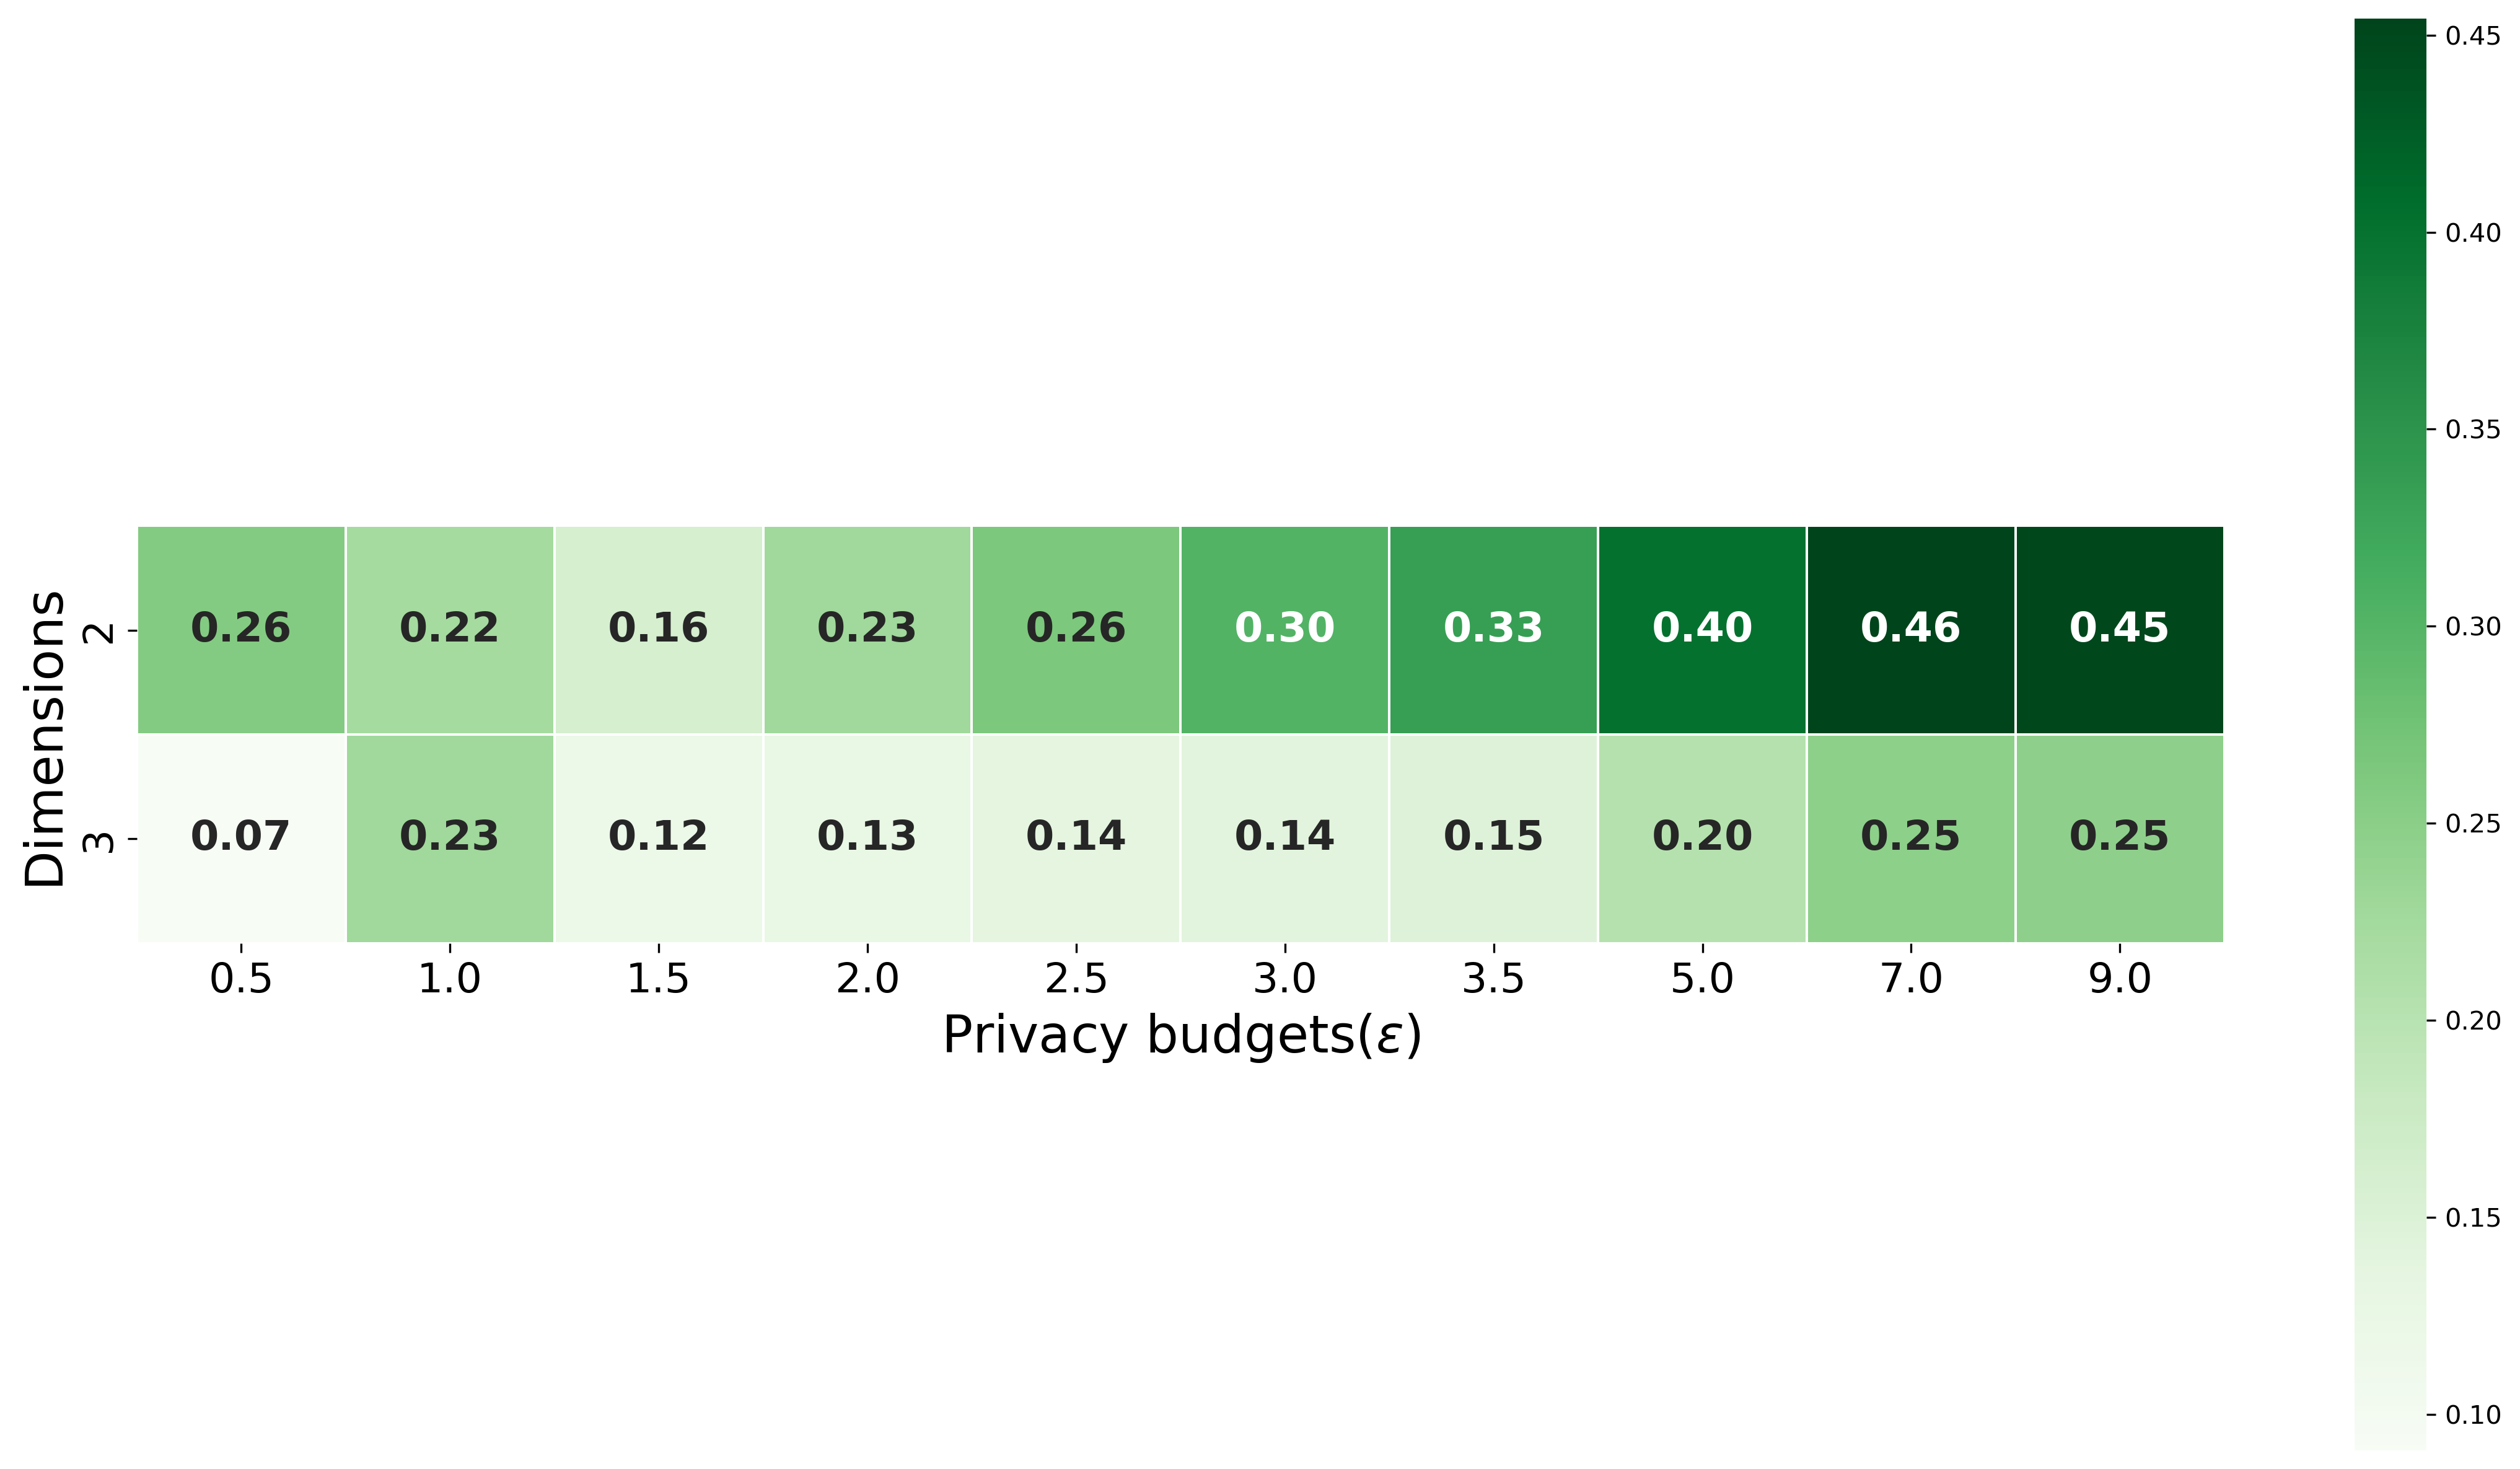
\includegraphics[width=1\textwidth]{Results/nd-laplace/nd-Laplace/circle-dataset/tpr.png}
            \label{fig:privacy_tpr_circle-dataset_adversial_advantage_kd-laplace}
        \end{subfigure}
        \vfill % vertical space

        \begin{subfigure}[c]{1\textwidth}
            \caption{\textbf{Heatmap TPR for the Piecewise mechanism, per privacy budget \& dimension for Circle-dataset.}}
            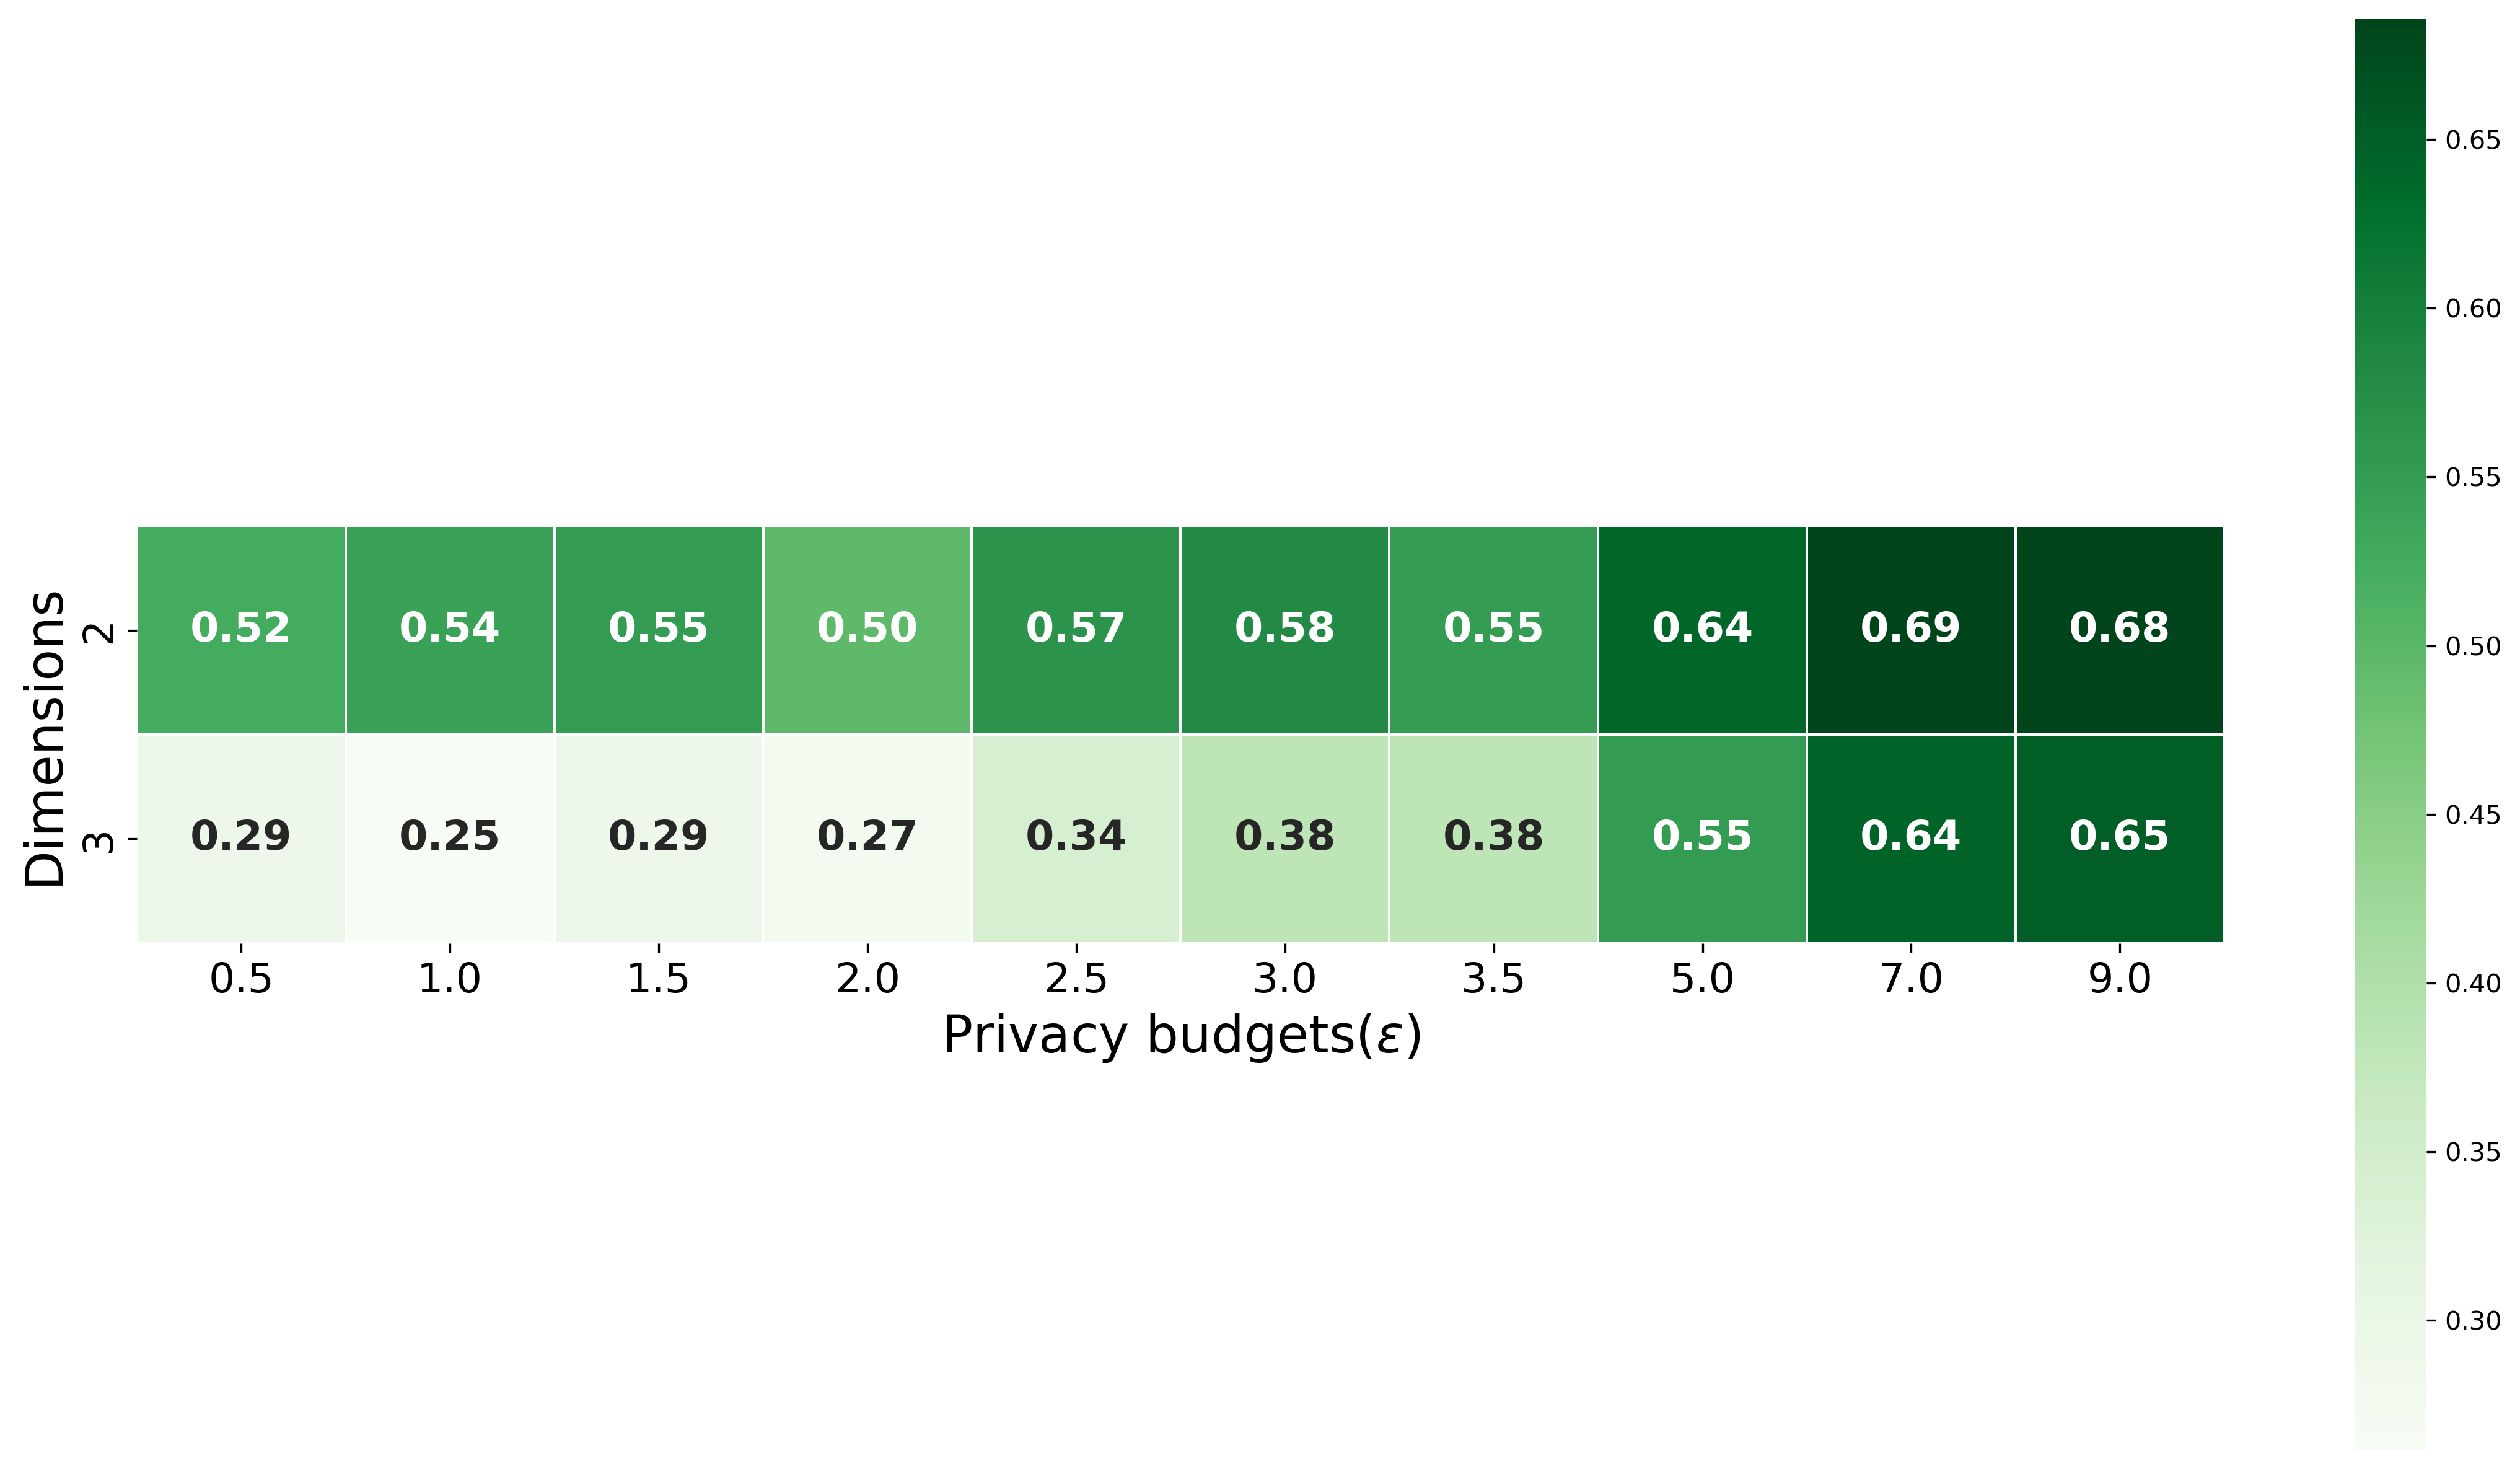
\includegraphics[width=1\textwidth]{Results/nd-laplace/piecewise/circle-dataset/tpr.png}
            \label{fig:privacy_tpr_circle-dataset_adversial_advantage_piecewise}
        \end{subfigure}
    \end{subfigure}
\end{figure}
For the nD-Laplace mechanism, it's again evident that the privacy budgets and dimensions influence the \gls{tpr}. The 2-dimensional data leaks more information than the 3-dimensional data. The same pattern is visible for the Piecewise mechanism, although the \gls{tpr} in this case is on average 0.10 higher compared to the nD-Laplace mechanism.
Given the \gls{ami} score, this makes sense since the Piecewise mechanism scored much higher (meaning: it's more similar to the original) than the nD-Laplace mechanism. Thus, the information leakage of the real data is higher.
{\todo[inline]{Why is 2-dimensional so much higher?}}
\newpage
\subsection{Line dataset}
\begin{figure}[H]
  \centering
  \begin{subfigure}[b]{0.80\textwidth}
    \begin{subfigure}[c]{1\textwidth}
      \caption{\textbf{Heatmap showing adversary advantage for the kD-Laplace mechanism, per privacy budget \& dimension for seeds-dataset.}}
      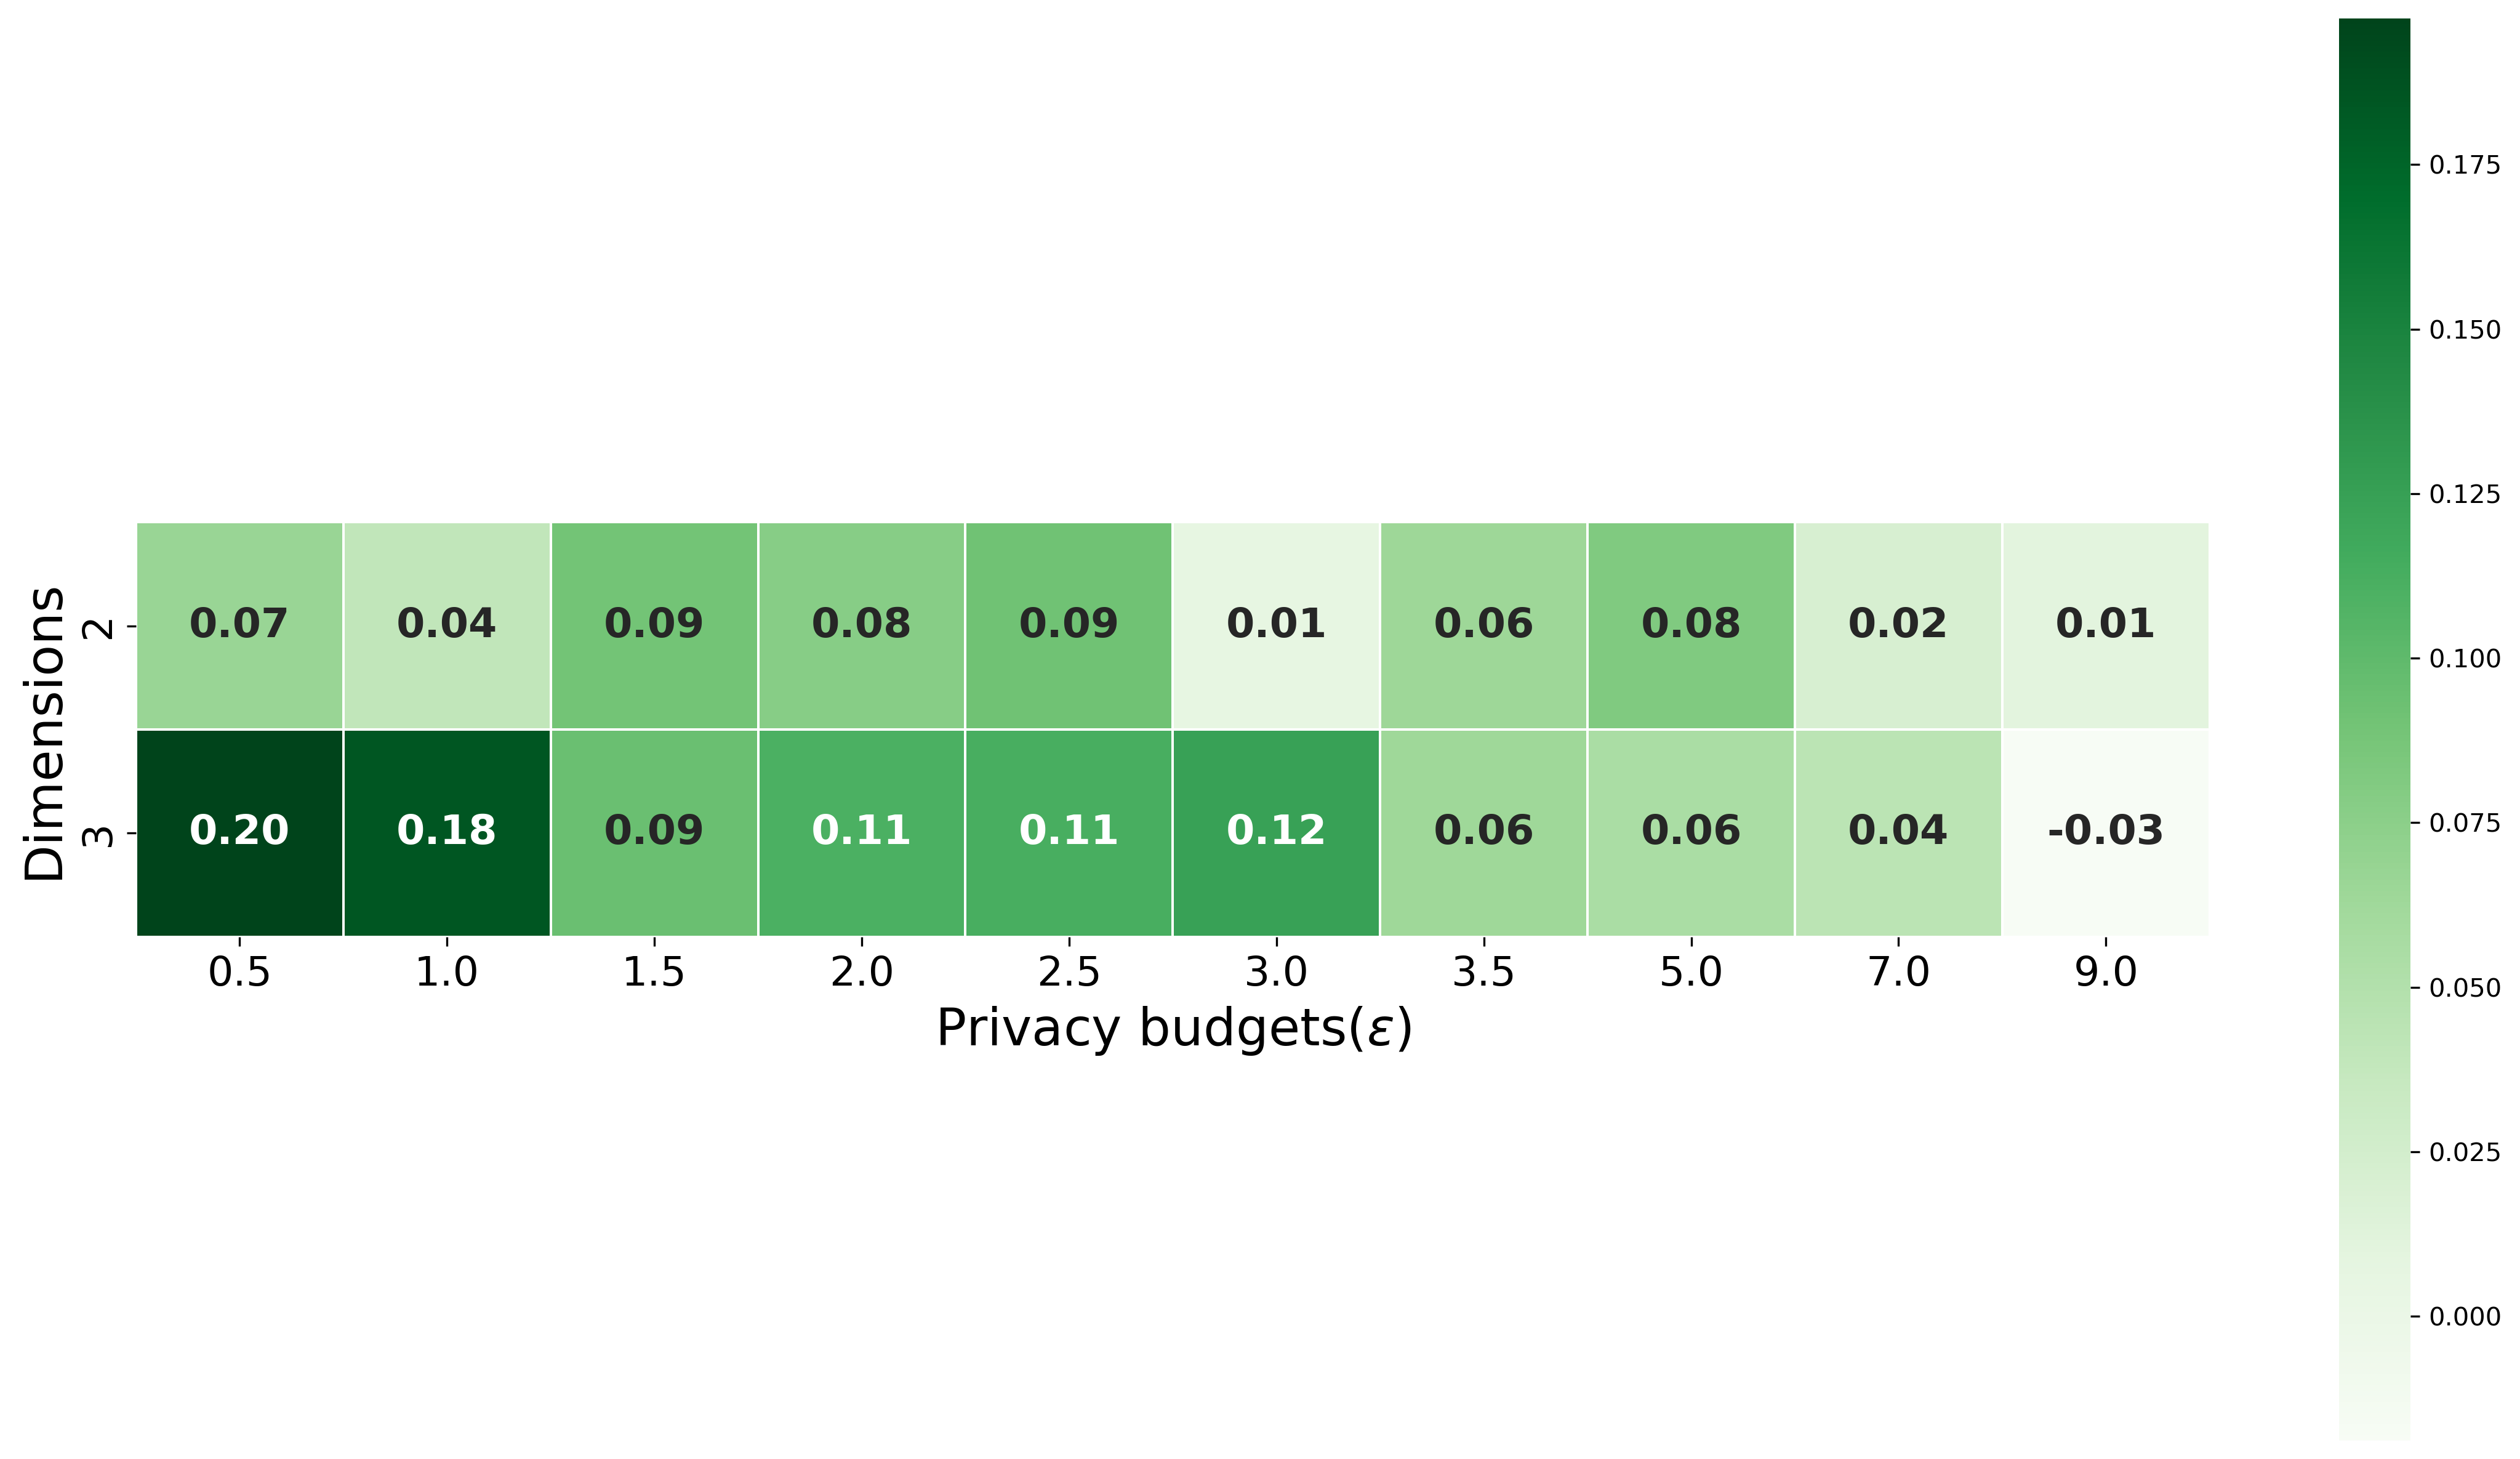
\includegraphics[width=1\textwidth]{Results/nd-laplace/nd-Laplace/line-dataset/attack_adv.png}
      \label{fig:privacy_line-dataset_adversial_advantage_kd-laplace}
    \end{subfigure}
    \vfill % vertical space

    \begin{subfigure}[c]{1\textwidth}
      \caption{\textbf{Heatmap showing adversary advantage for the Piecewise mechanism, per privacy budget \& dimension for seeds-dataset.}}
      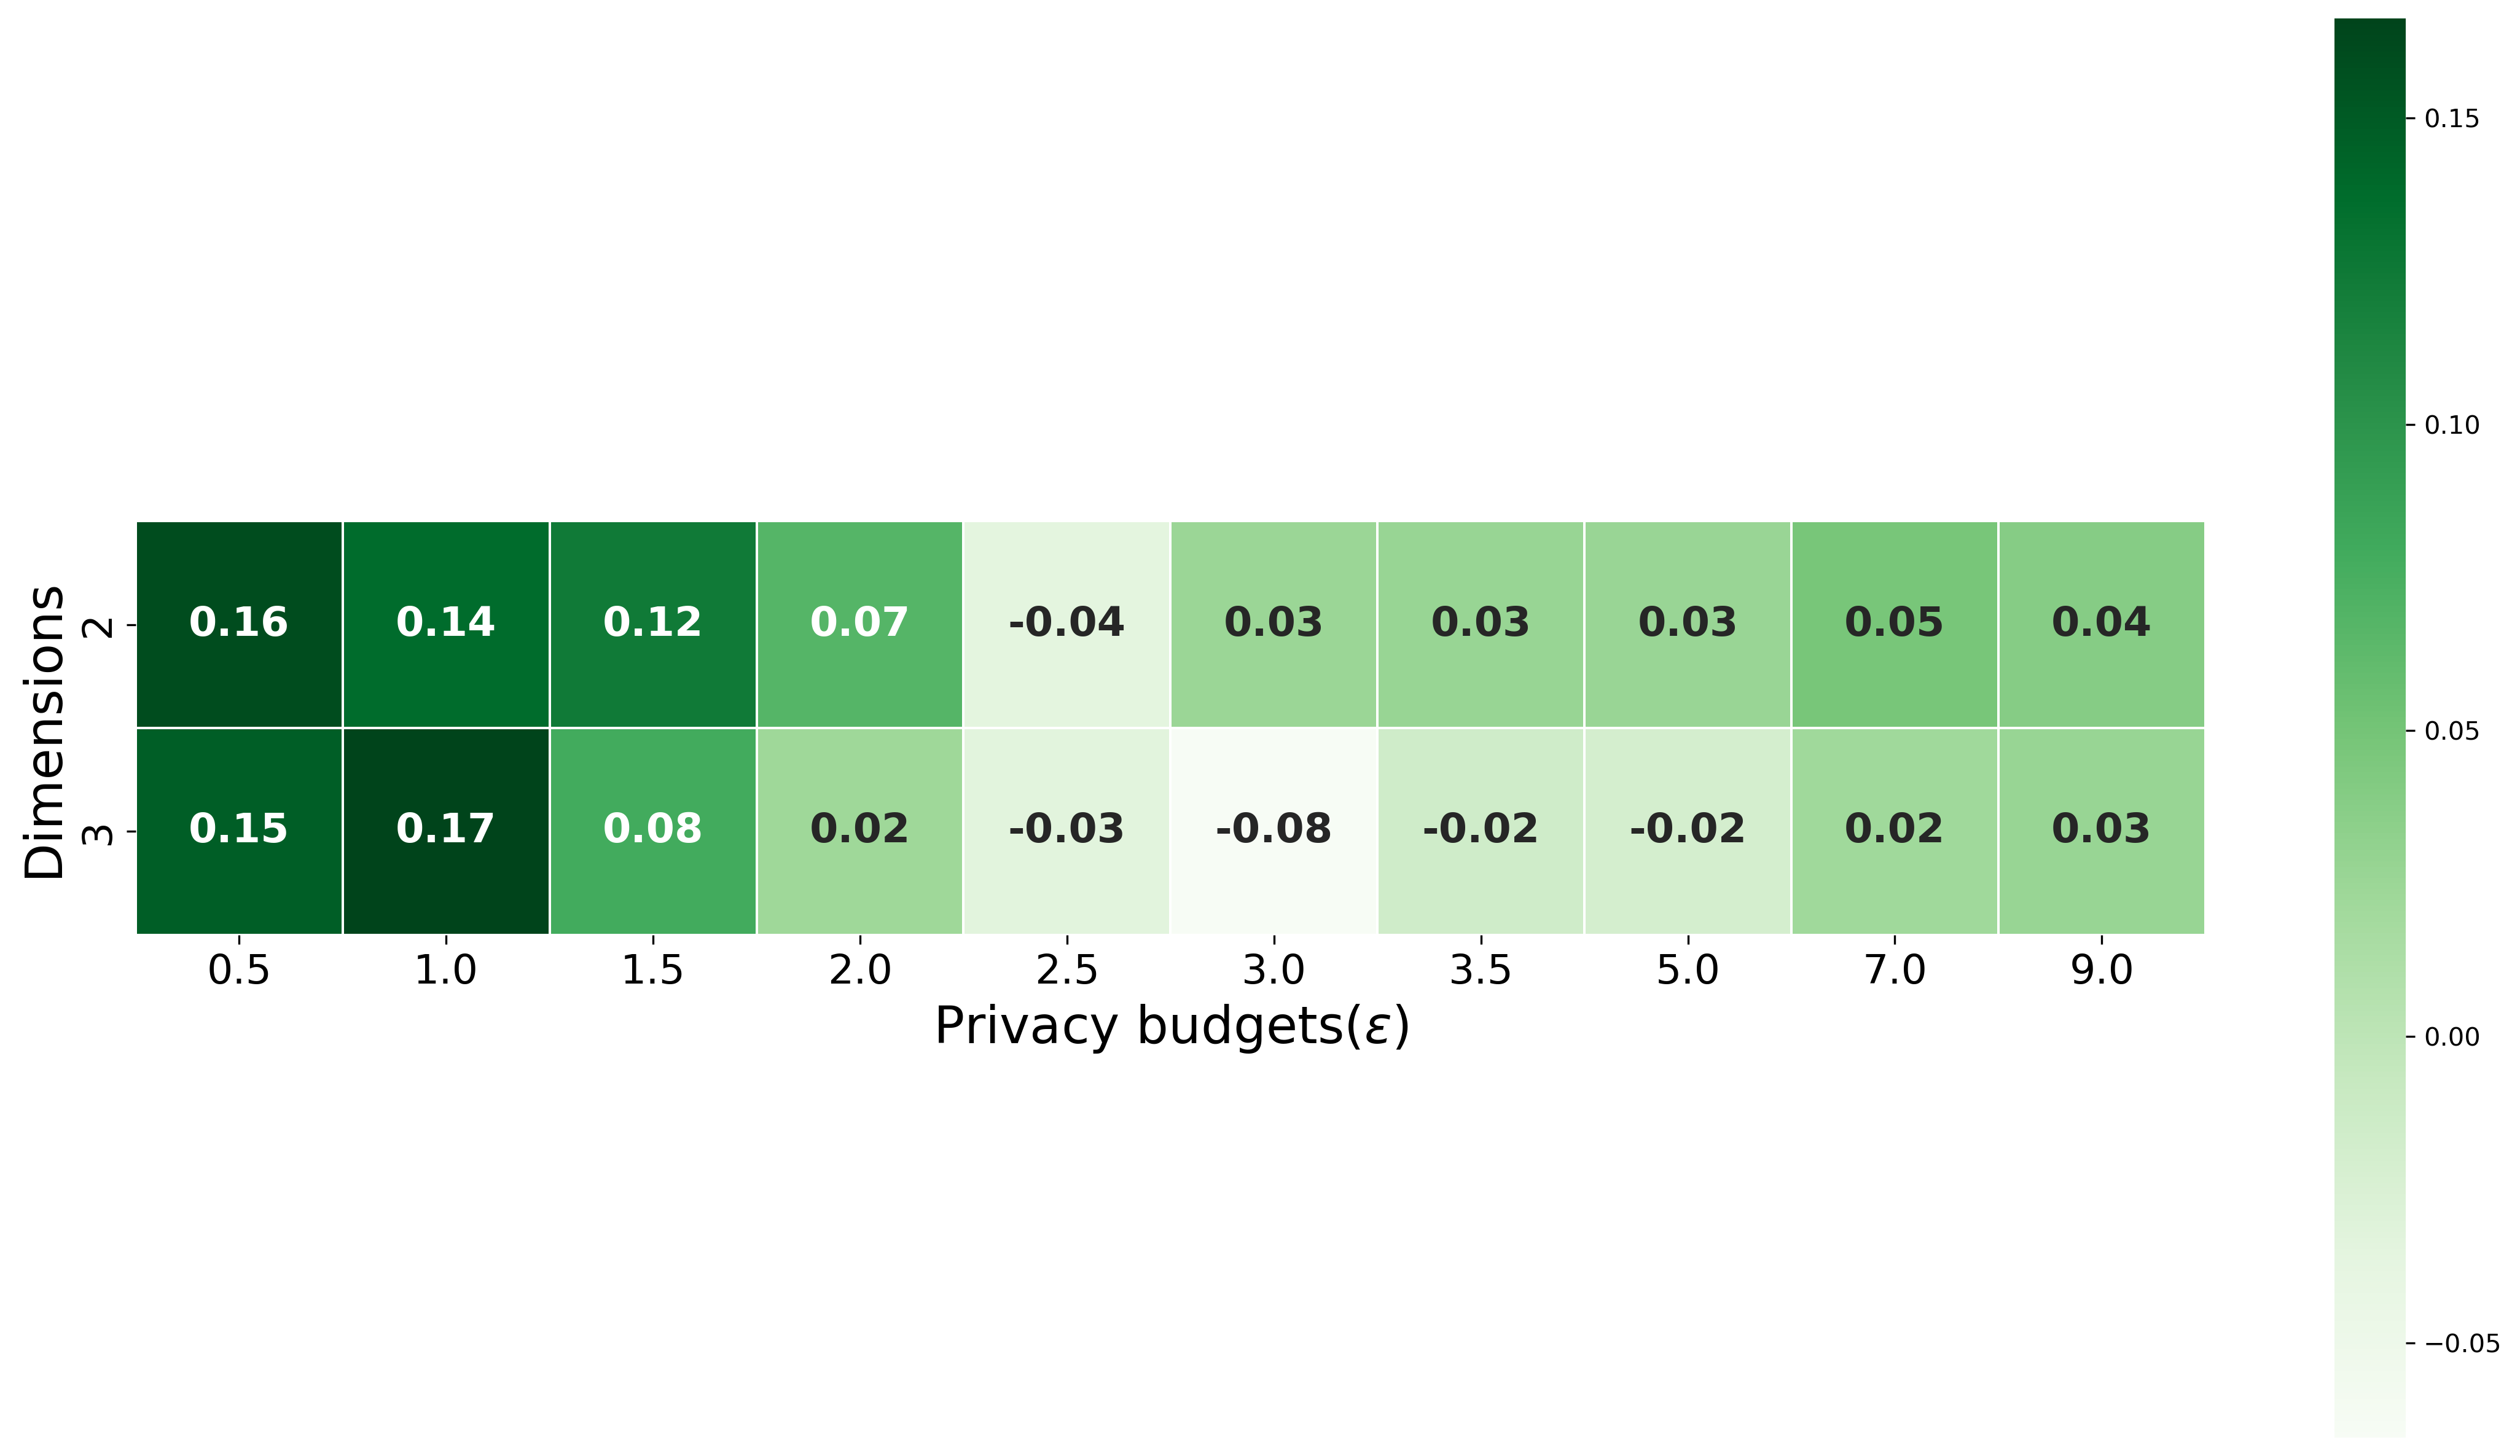
\includegraphics[width=1\textwidth]{Results/nd-laplace/piecewise/line-dataset/attack_adv.png}
      \label{fig:privacy_line-dataset_adversial_advantage_piecewise}
    \end{subfigure}
  \end{subfigure}
\end{figure}
The nD-Laplace mechanism shows similar results to what we've seen before from the other membership advantage scores. Notably here, the 2-dimensional data scores better (lower) this time than the 3-dimensional data. Whereas in the other plots, the 2-dimensional data leaked a lot of information.
The Piecewise mechanism does show a slightly higher membership advantage for 2-dimensional data.
In general, we again see the pattern that the membership advantage is higher for the lower privacy budgets, even though we expected the opposite.
\todo[inline]{Analyze why 2-dimensional data performs better this time}.
Therefore, we will also look at the \gls{tpr} on the next page again to get a better understanding of the underlying information.
\newpage
\begin{figure}[H]
    \centering
    \begin{subfigure}[b]{0.9\textwidth}
        \begin{subfigure}[c]{1\textwidth}
            \caption{\textbf{Heatmap TPR for the kD-Laplace mechanism, per privacy budget \& dimension for line-dataset.}}
            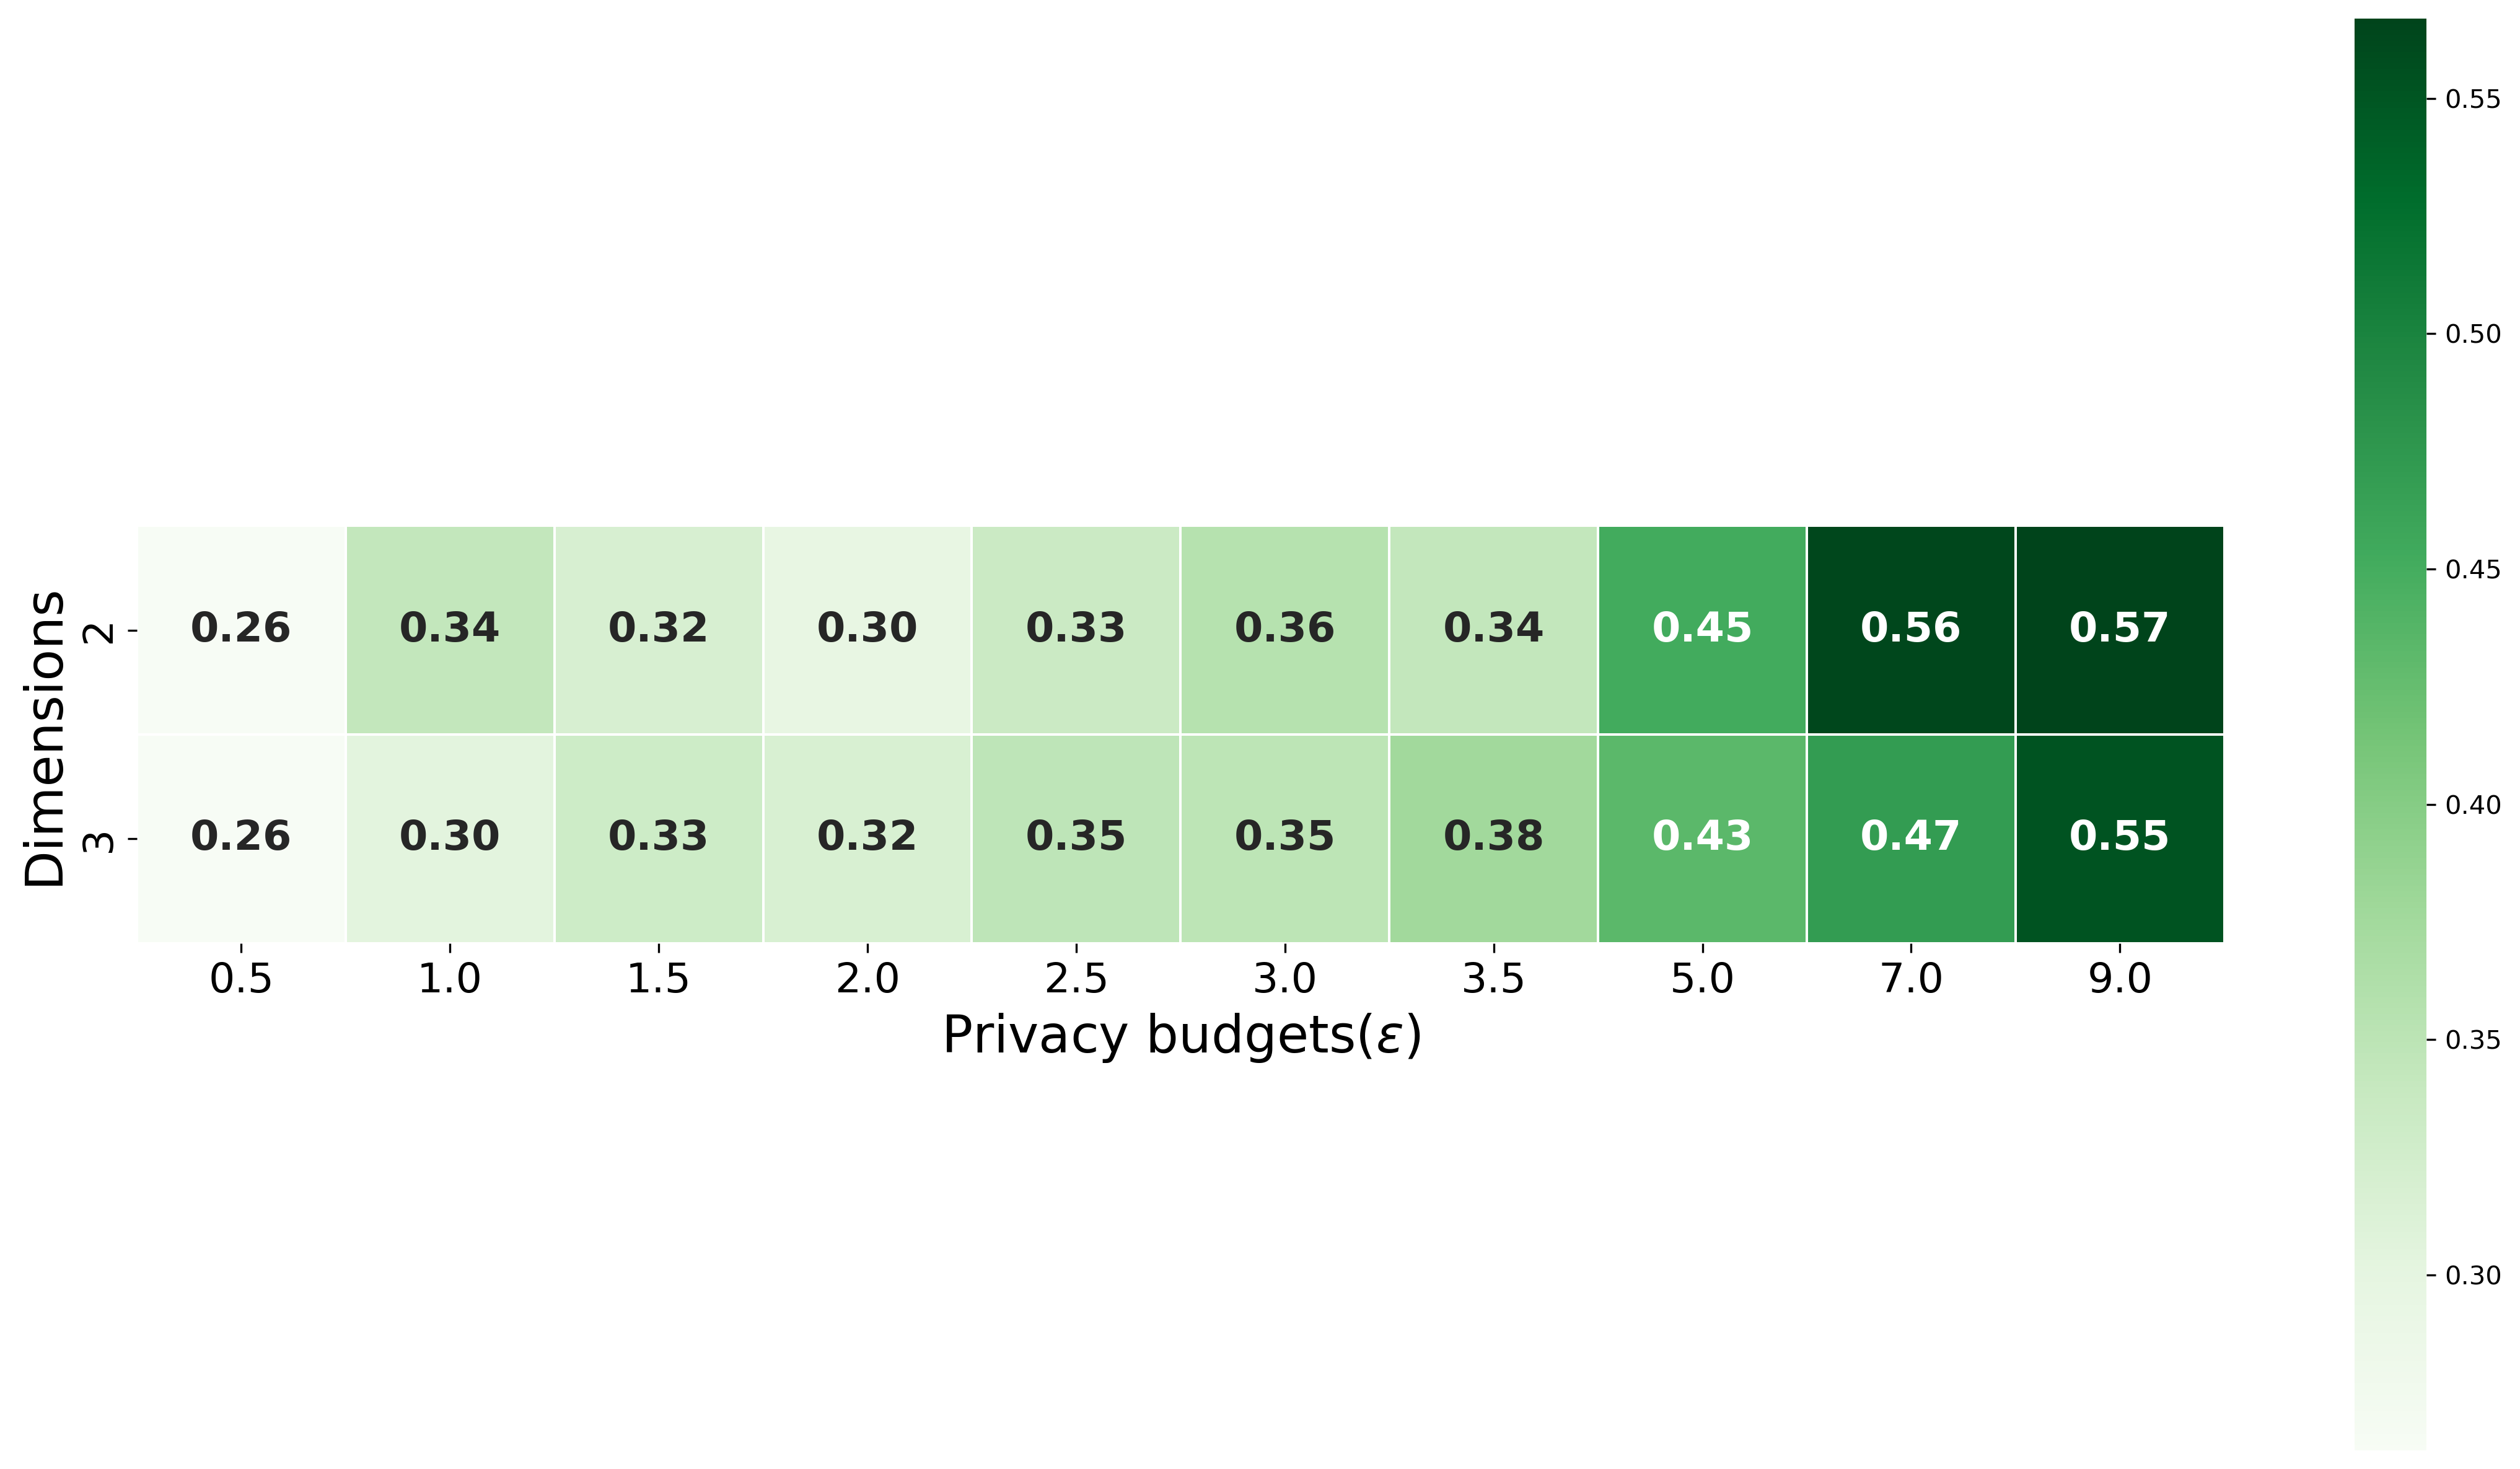
\includegraphics[width=1\textwidth]{Results/nd-laplace/nd-Laplace/line-dataset/tpr.png}
            \label{fig:privacy_tpr_line-dataset_adversial_advantage_kd-laplace}
        \end{subfigure}
        \vfill % vertical space

        \begin{subfigure}[c]{1\textwidth}
            \caption{\textbf{Heatmap TPR for the Piecewise mechanism, per privacy budget \& dimension for line-dataset.}}
            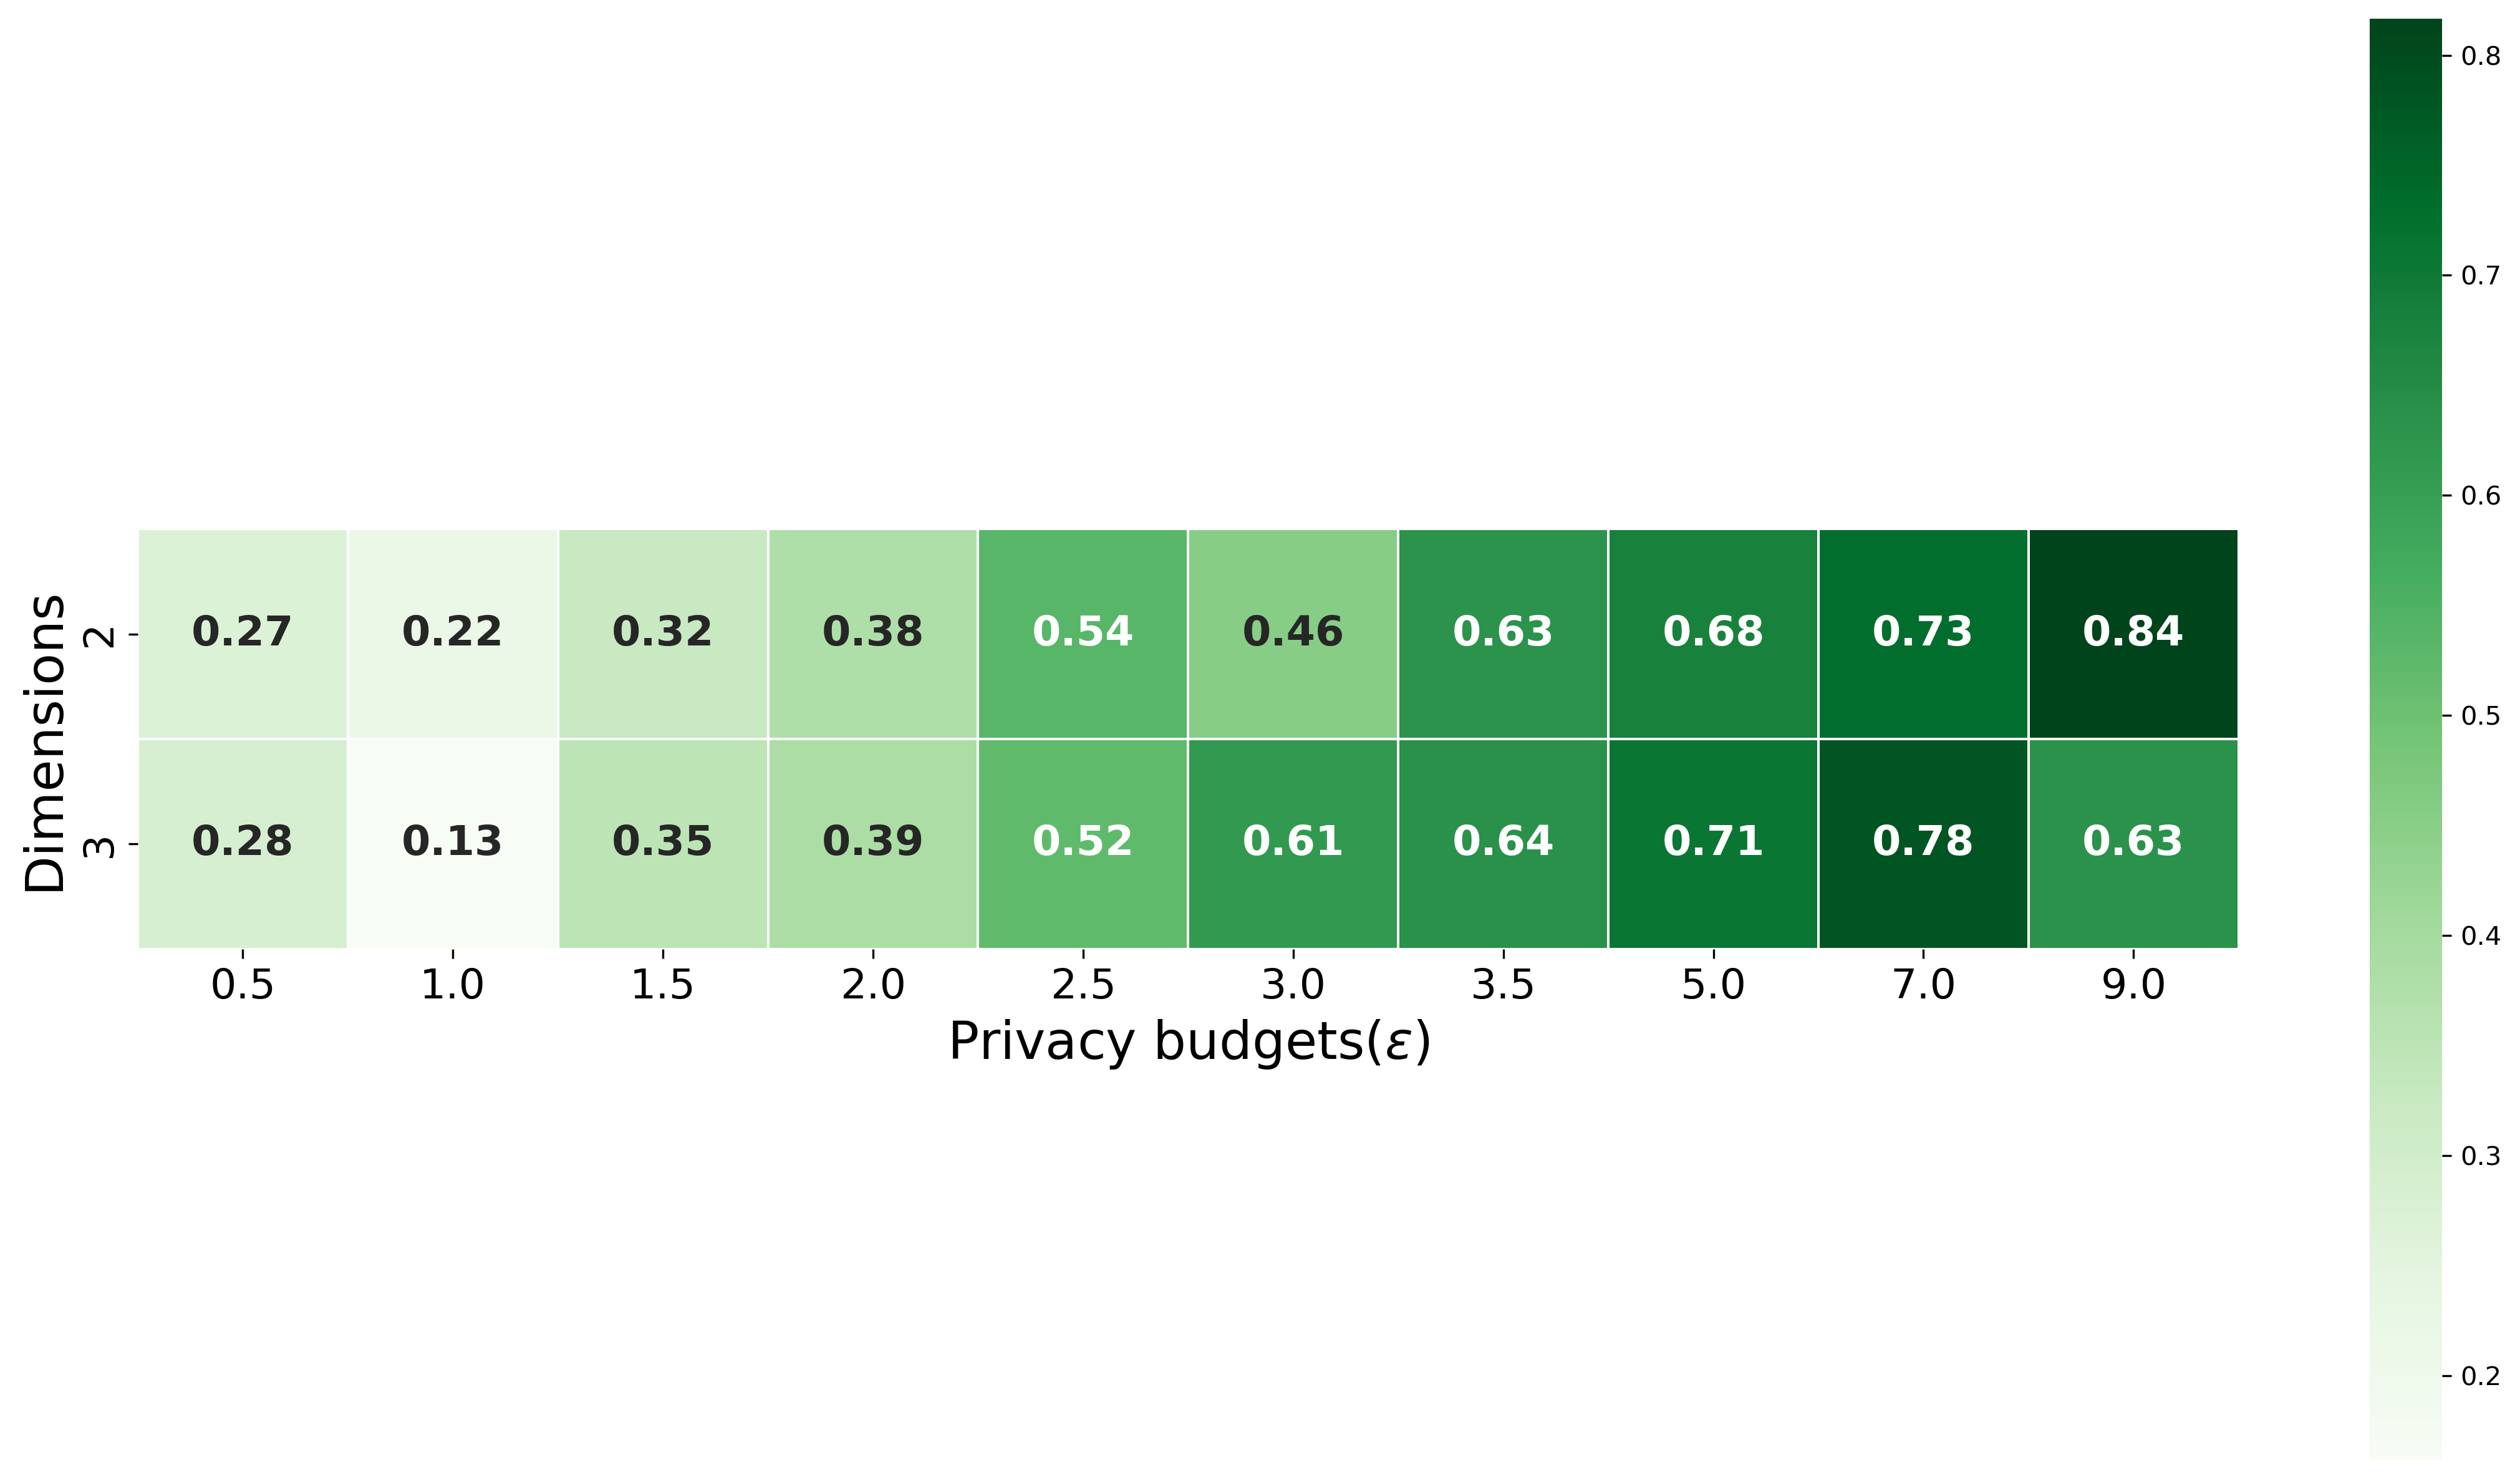
\includegraphics[width=1\textwidth]{Results/nd-laplace/piecewise/line-dataset/tpr.png}
            \label{fig:privacy_tpr_line-dataset_adversial_advantage_piecewise}
        \end{subfigure}
    \end{subfigure}
\end{figure}
The heatmaps above show a similar result to the other plots, where there is a logical progression of a low membership advantage for lower privacy budgets and, on the other hand, a higher one for higher privacy budgets.
The nD-Laplace scores a lower membership advantage, which is consistent with the \gls{ami} score that is also low.
The reason the \gls{tpr} is higher than, for example, the circle-dataset, is because the Piecewise mechanism is good at preserving the shape of the line-data \ref{fig:validation-Line-dataset_comparison_2d-laplace}.}. 
\newpage
\subsection{Skewed dataset}
\begin{figure}[H]
  \centering
  \begin{subfigure}[b]{0.85\textwidth}
    \begin{subfigure}[c]{1\textwidth}
      \caption{\textbf{Heatmap showing adversary advantage for the kD-Laplace mechanism, per privacy budget \& dimension for seeds-dataset.}}
      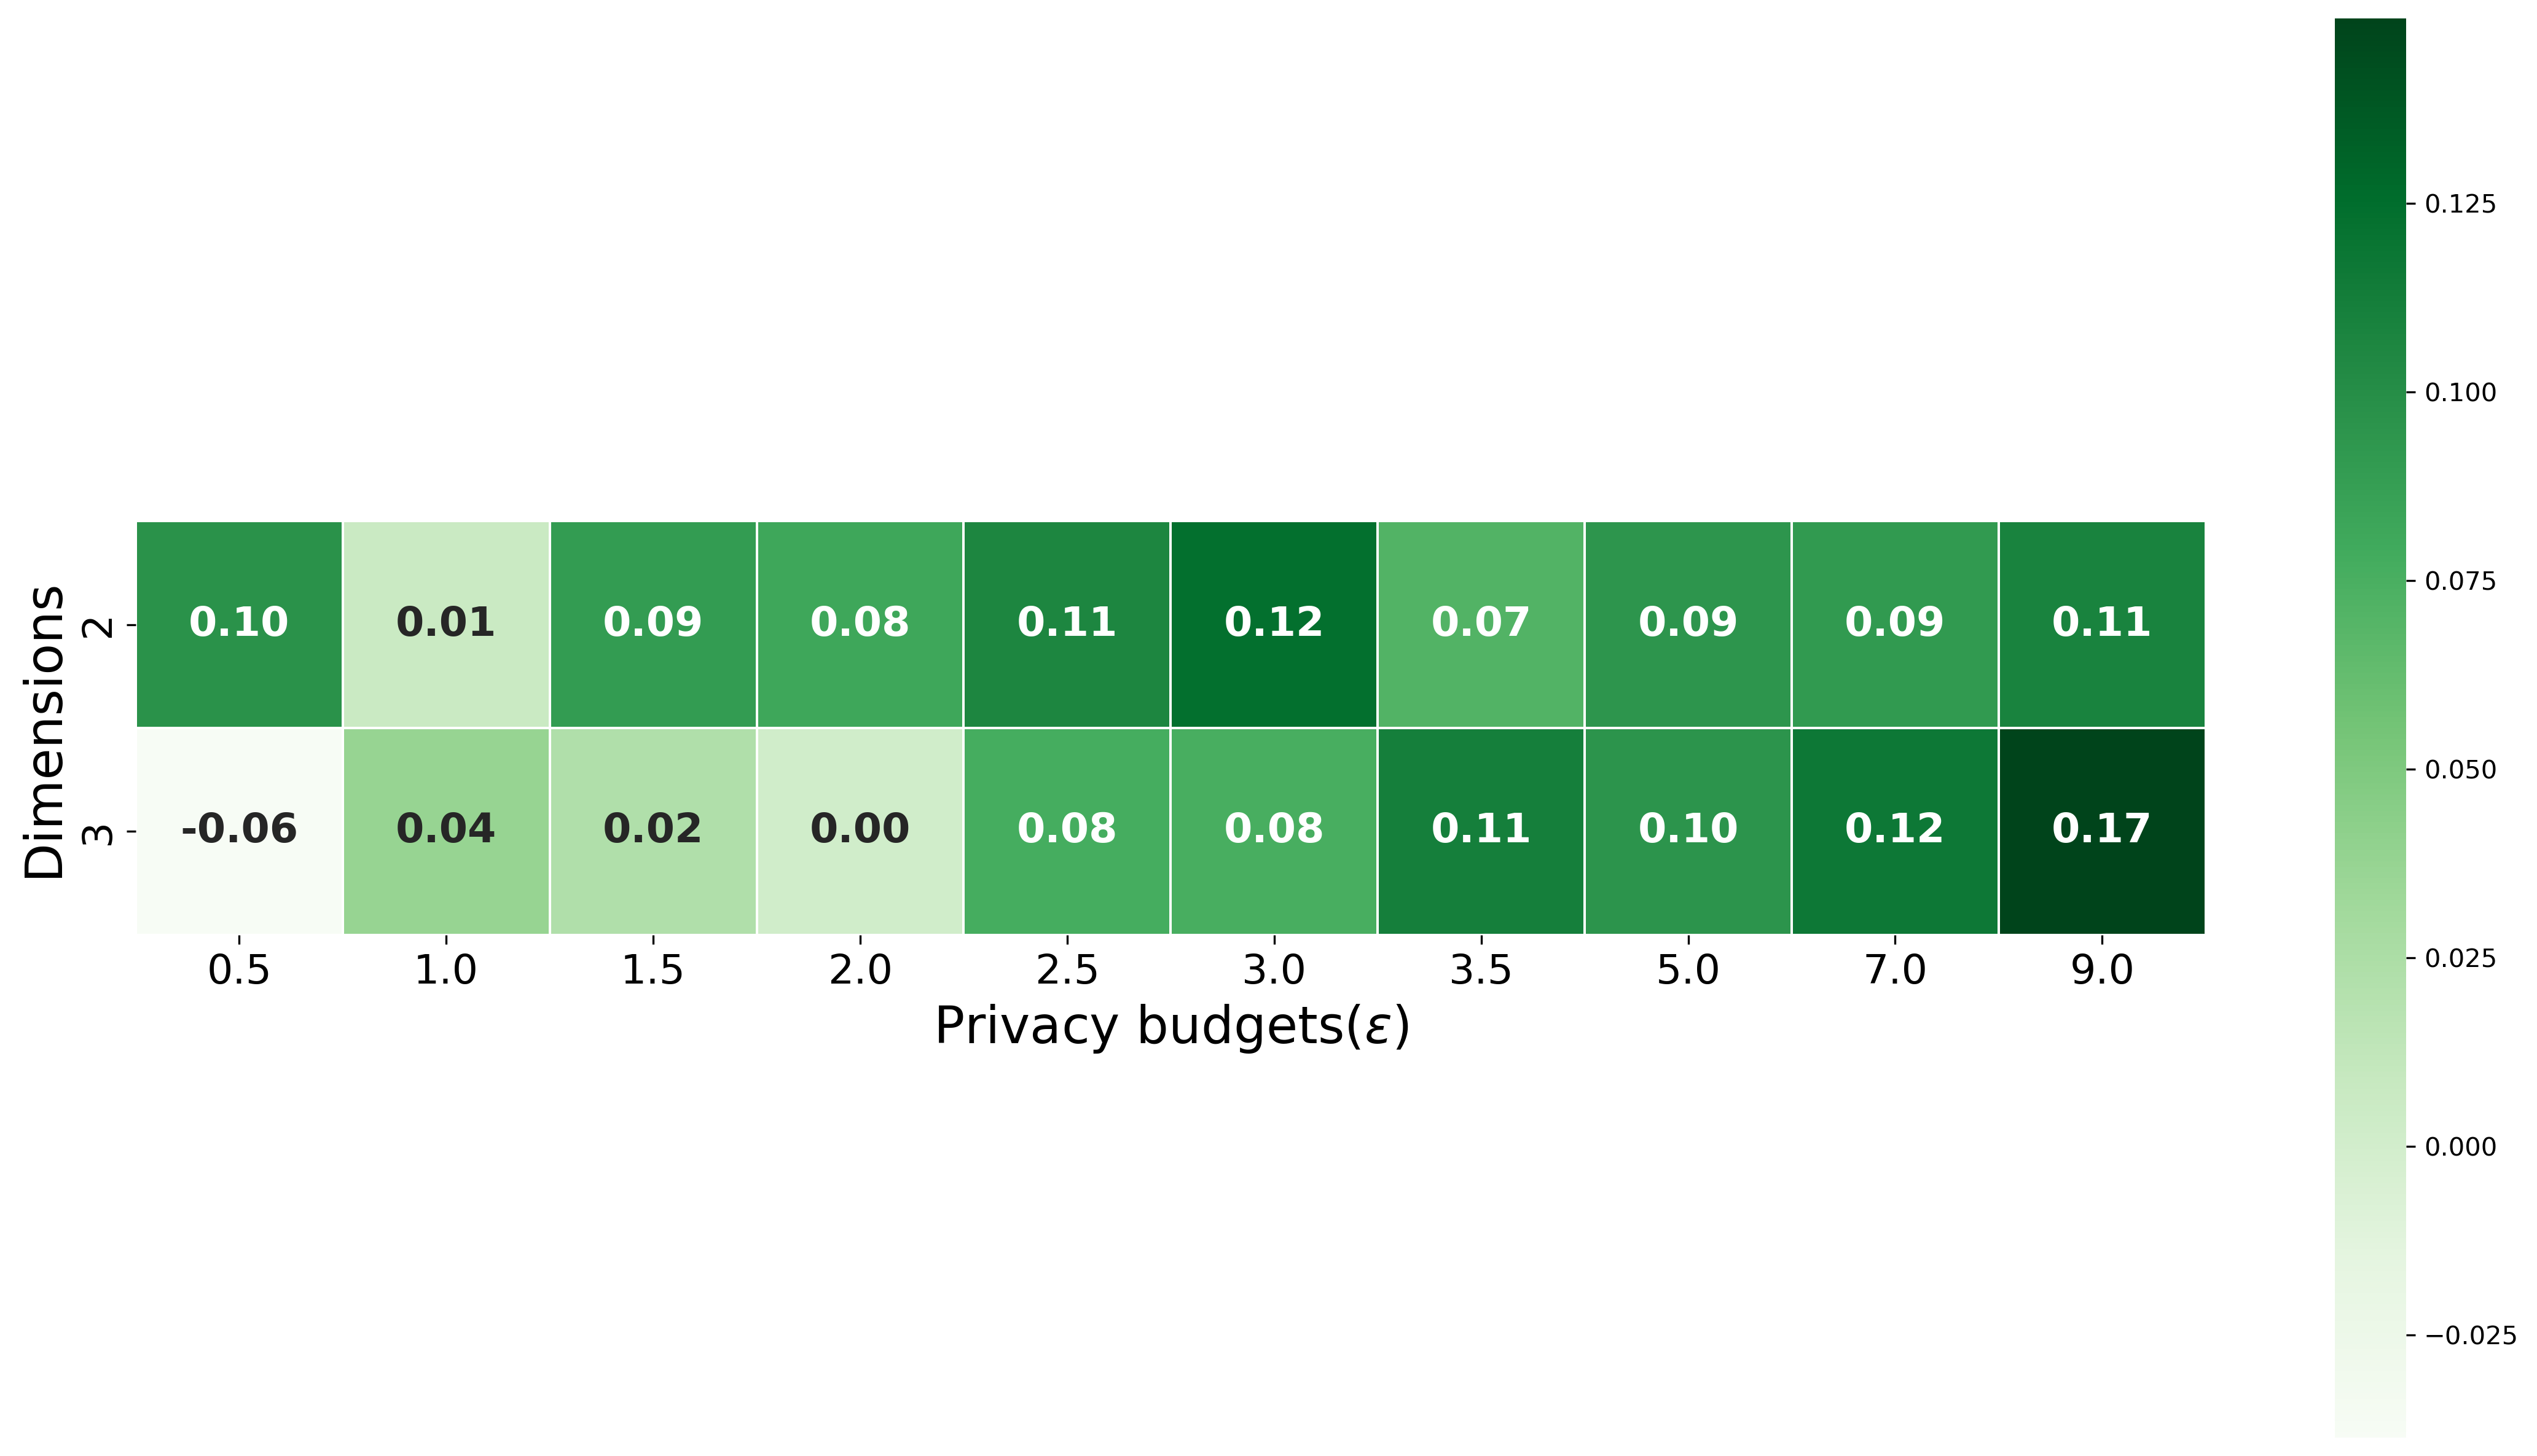
\includegraphics[width=1\textwidth]{Results/nd-laplace/nd-Laplace/skewed-dataset/attack_adv.png}
      \label{fig:privacy_skewed-dataset_adversial_advantage_kd-laplace}
    \end{subfigure}
    \vfill % vertical space

    \begin{subfigure}[c]{1\textwidth}
      \caption{\textbf{Heatmap showing adversary advantage for the Piecewise mechanism, per privacy budget \& dimension for seeds-dataset.}}
      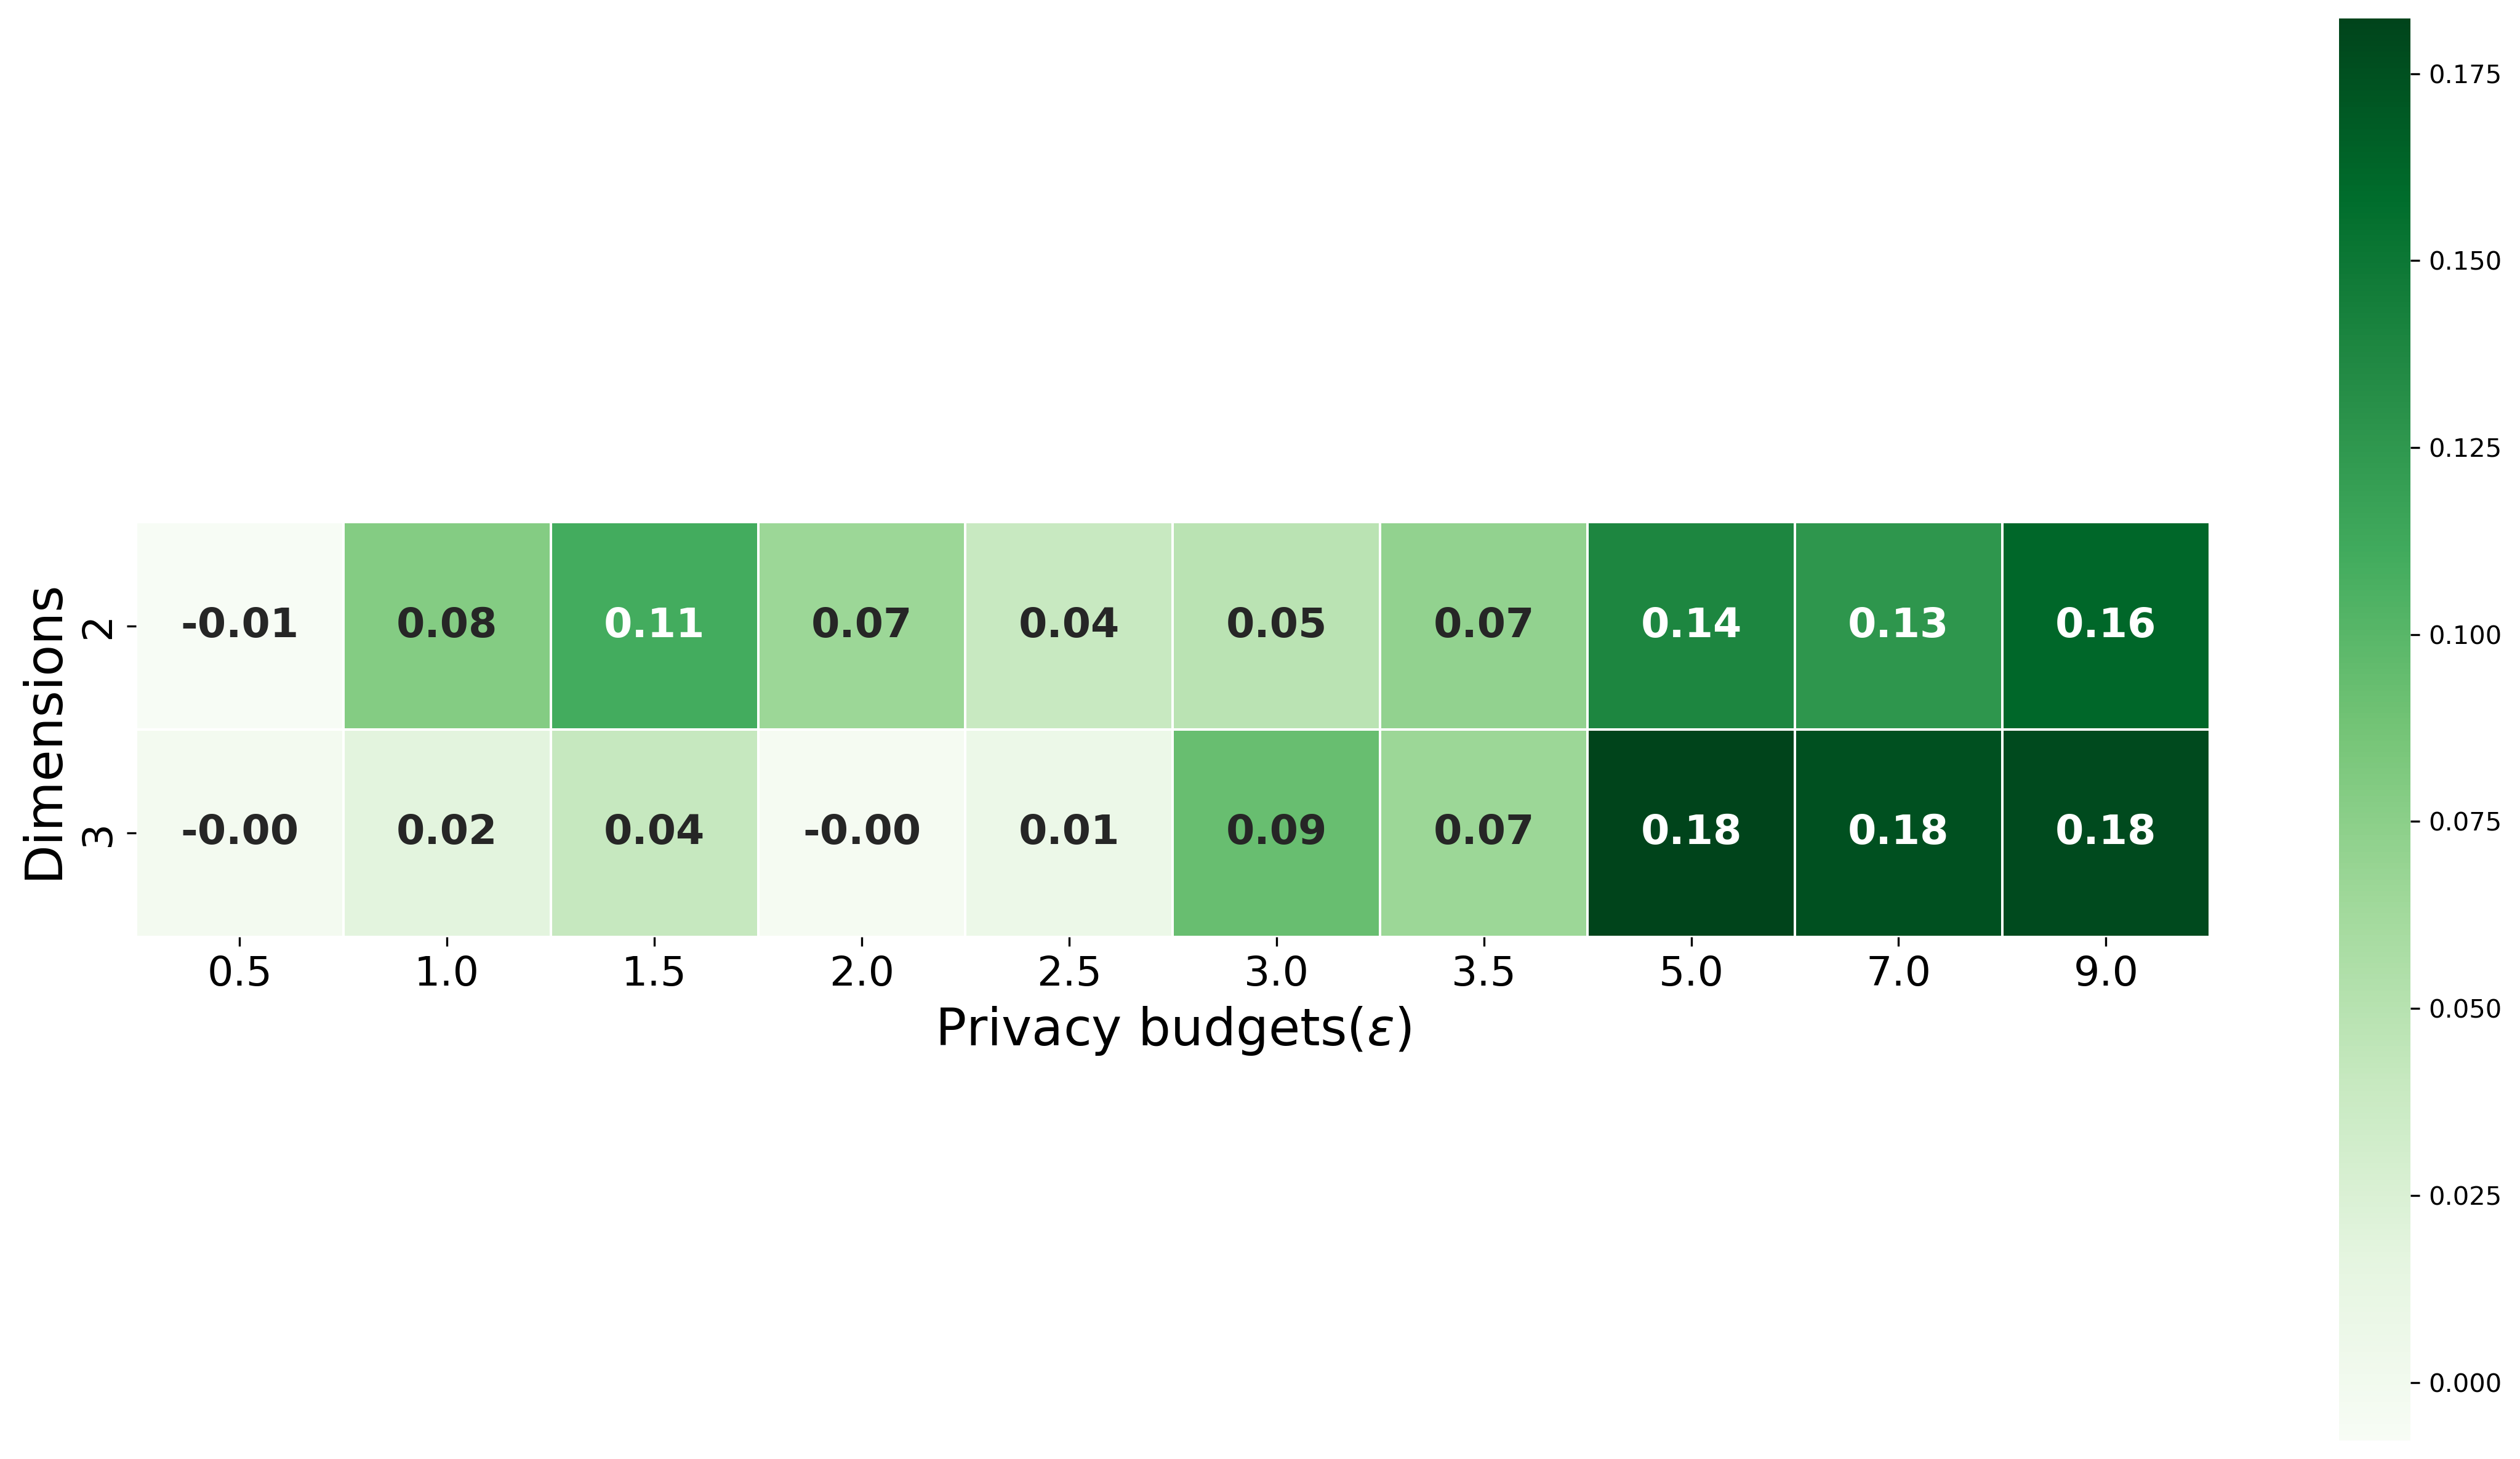
\includegraphics[width=1\textwidth]{Results/nd-laplace/piecewise/skewed-dataset/attack_adv.png}
      \label{fig:privacy_skewed-dataset_adversial_advantage_piecewise}
    \end{subfigure}
  \end{subfigure}
\end{figure}
\newpage
\subsection{Mechanism comparison}
In this section, we compare the different mechanisms for each dataset.
For this purpose, we also include all the different variants of kd-Laplace to see if there is a difference between them.
So, instead of comparing the mechanisms based on the number of dimensions, we compare them on the average scores for all dimensions per mechanism.
We are most interested in the utility and performance, and to compare them, we only show the \gls{ami} and adversary advantage scores.
\todo[inline]{Also needs privacy distance comparison}.
\begin{figure}[H]
  \centering
  \begin{subfigure}{0.30\textwidth}
    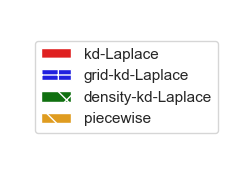
\includegraphics[width=\textwidth]{Results/kd-laplace/ami_bar_comparison_legend.png}
  \end{subfigure}
  \begin{subfigure}{1\textwidth}
    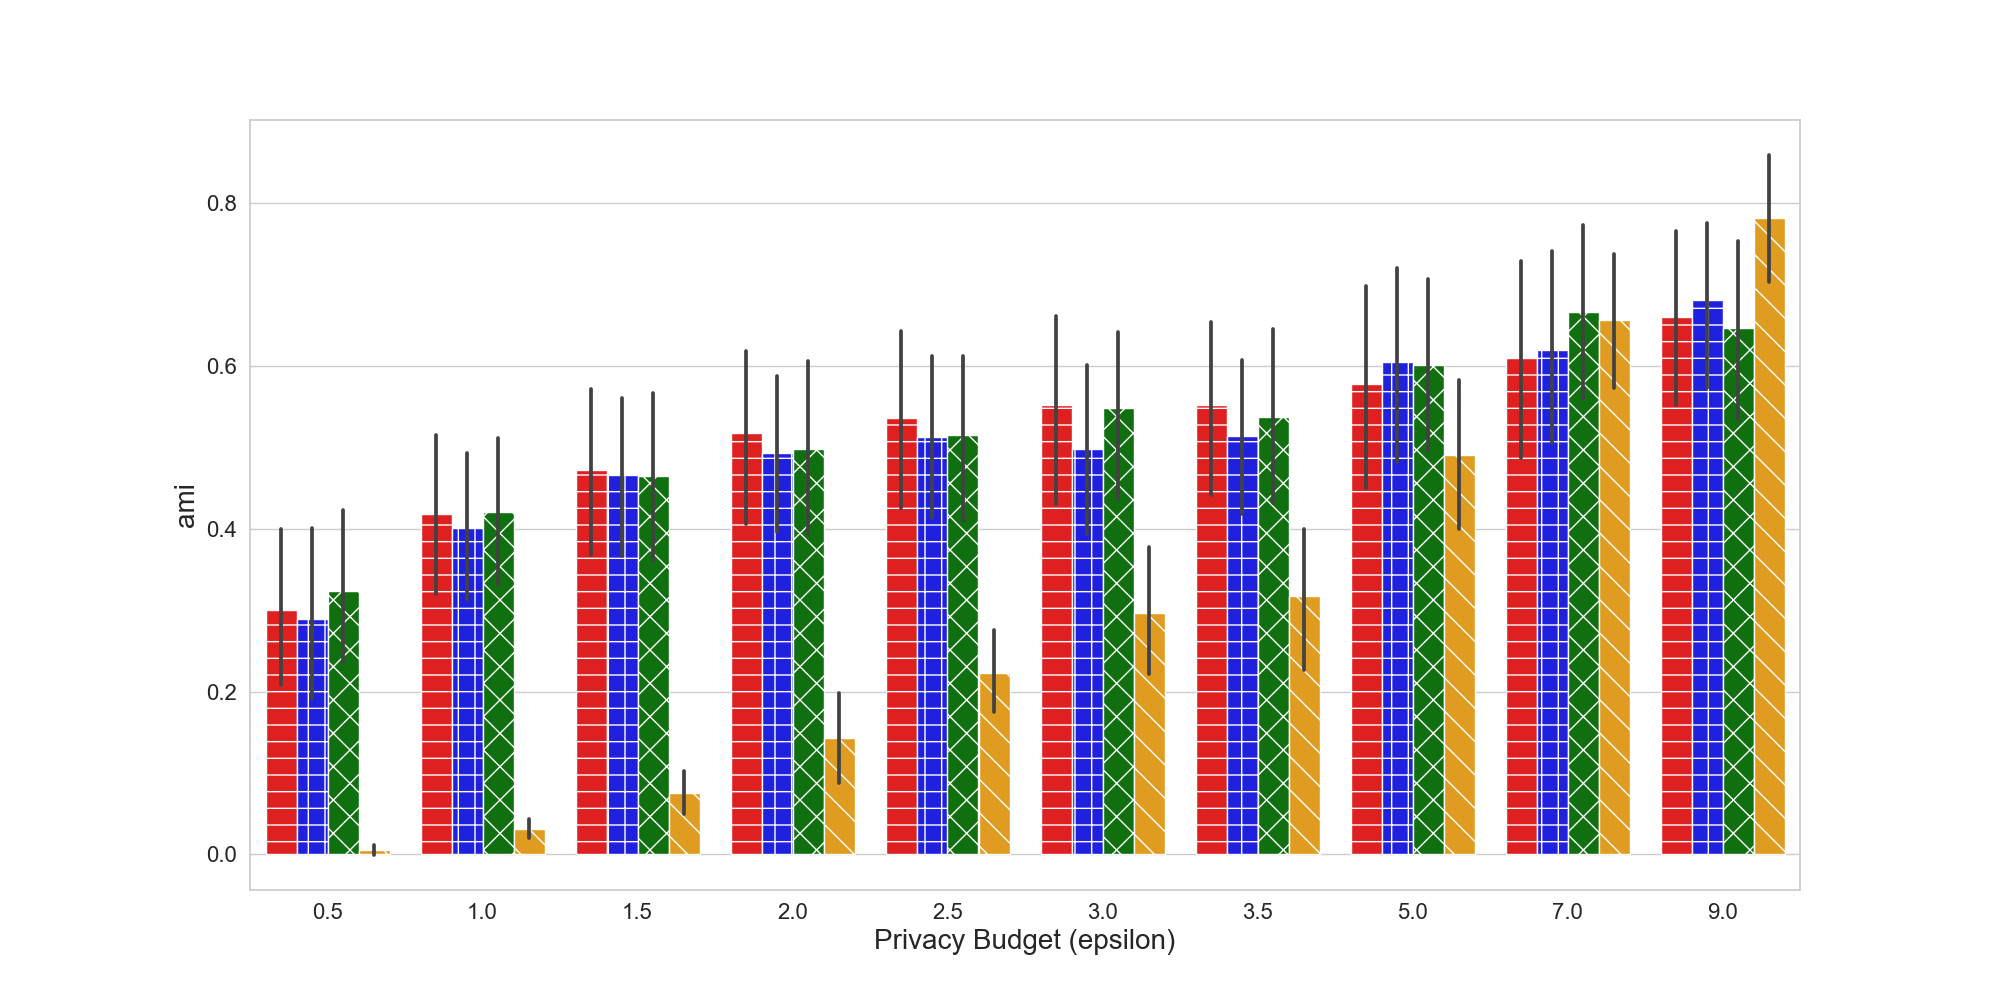
\includegraphics[width=1\textwidth]{Results/nd-laplace/ami_seeds-dataset_comparison.png}
  \end{subfigure}
  \begin{subfigure}{1\textwidth}
    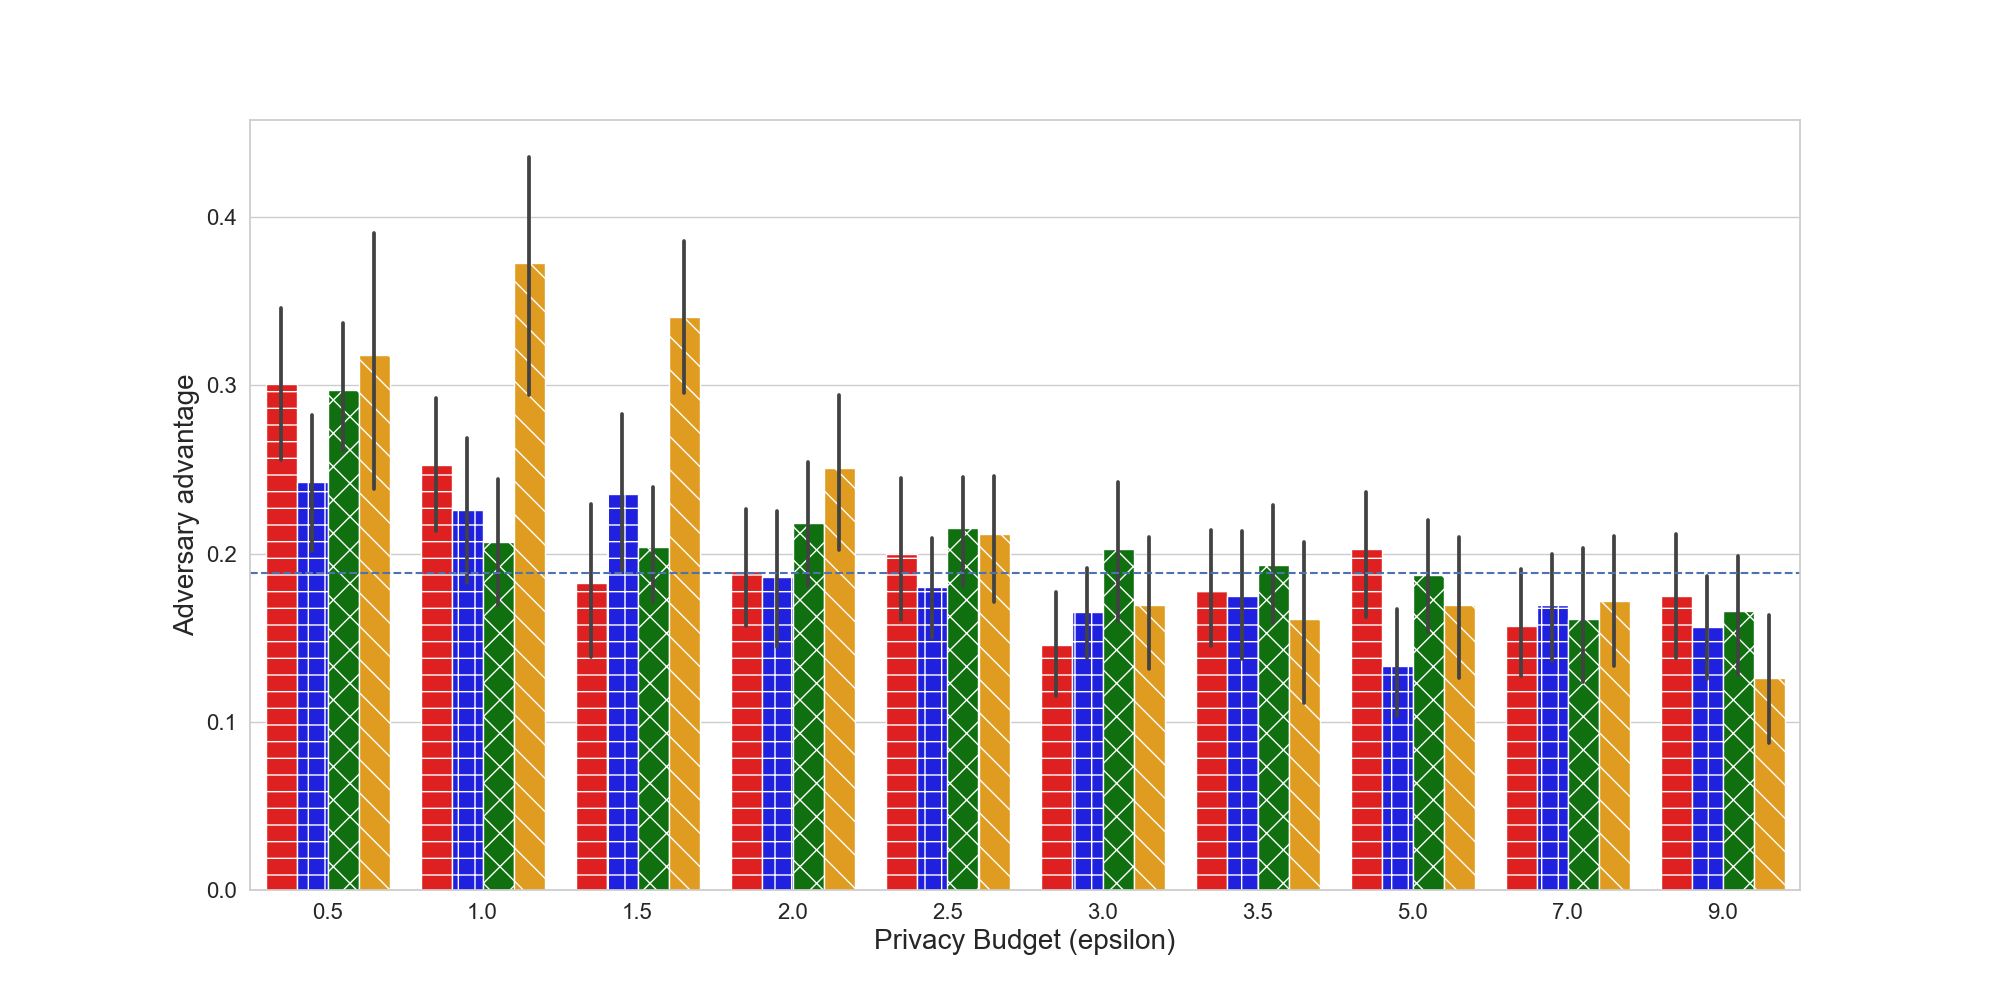
\includegraphics[width=1\textwidth]{Results/nd-laplace/attack_adv_seeds-dataset_comparison.png}
  \end{subfigure}
  \caption{Average AMI (top) and Adversary Advantage (bottom) comparison for each mechanism for seeds-dataset (8 dimensions).}
  \label{fig:utility_seeds-dataset_comparison_nd_plot}
\end{figure}
\todo[inline]{Add interpretation}
\newpage


\begin{figure}[H]
  \centering
  \begin{subfigure}{0.30\textwidth}
    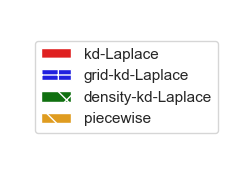
\includegraphics[width=\textwidth]{Results/kd-laplace/ami_bar_comparison_legend.png}
  \end{subfigure}
  \begin{subfigure}{1\textwidth}
    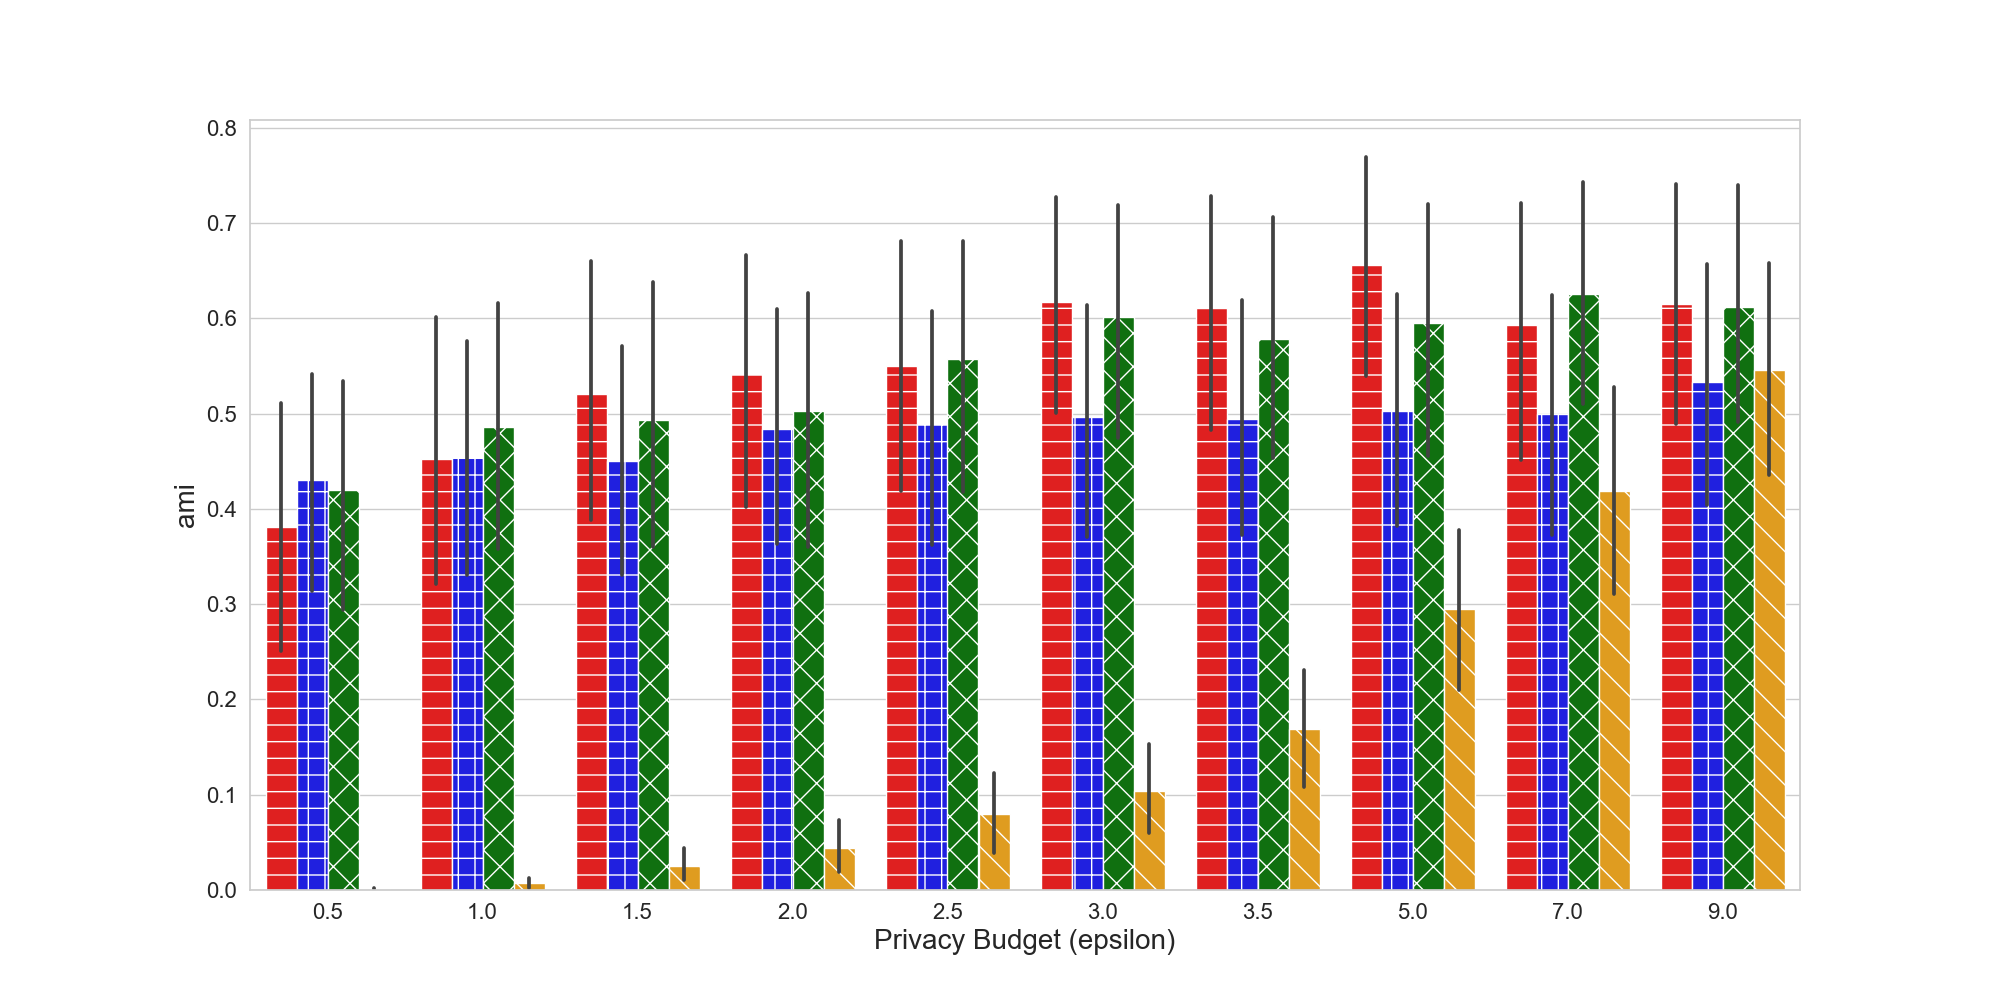
\includegraphics[width=1\textwidth]{Results/nd-laplace/ami_heart-dataset_comparison.png}
  \end{subfigure}
  \begin{subfigure}{1\textwidth}
    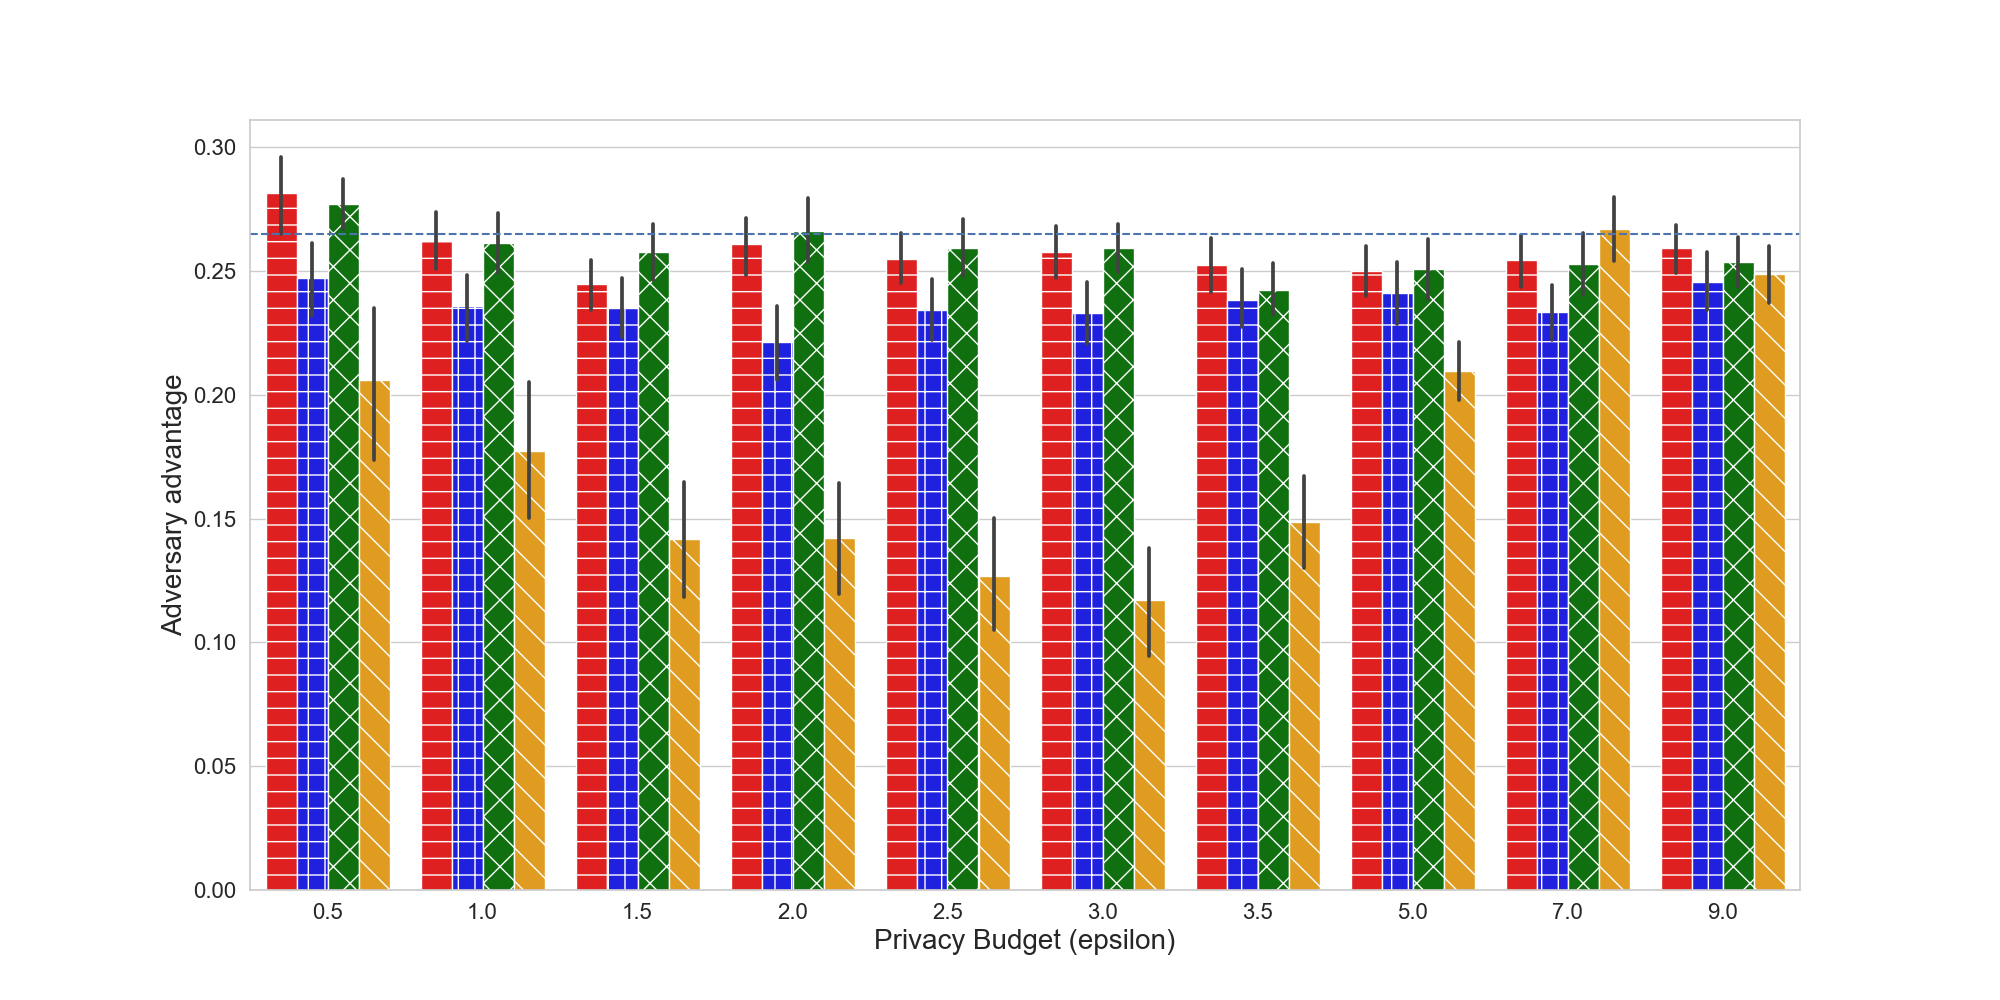
\includegraphics[width=1\textwidth]{Results/nd-laplace/attack_adv_heart-dataset_comparison.png}
  \end{subfigure}
  \caption{Average AMI (top) and Adversary Advantage (bottom) comparison for each mechanism for heart-dataset (10 dimensions).}
  \label{fig:utility_heart-dataset_comparison_nd_plot}
\end{figure}
\todo[inline]{Add interpretation}
\newpage

\subsection{Shape datasets}

\begin{figure}[H]
  \centering
  \begin{subfigure}{0.30\textwidth}
    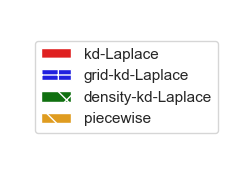
\includegraphics[width=\textwidth]{Results/kd-laplace/ami_bar_comparison_legend.png}
  \end{subfigure}
  \begin{subfigure}{1\textwidth}
    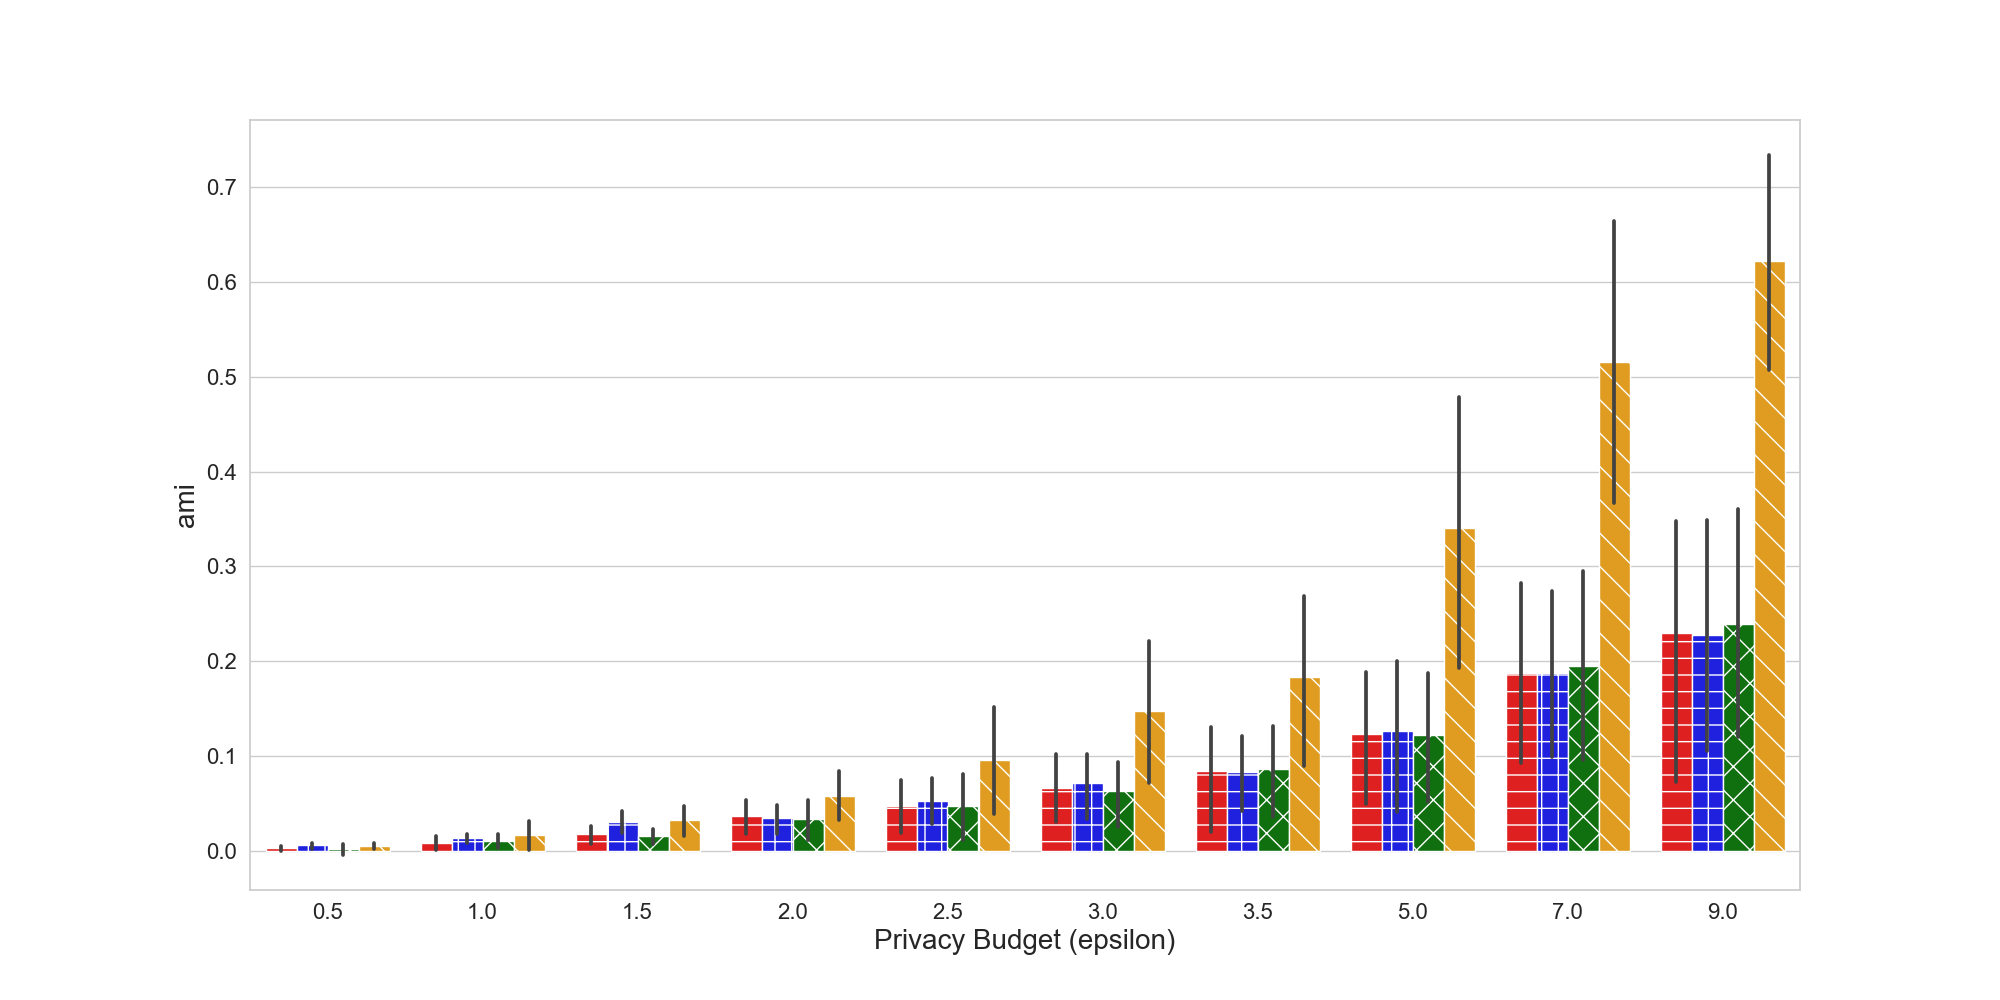
\includegraphics[width=1\textwidth]{Results/nd-laplace/ami_circle-dataset_comparison.png}
  \end{subfigure}
  \begin{subfigure}{1\textwidth}
    \includegraphics[width=1\textwidth]{Results/nd-laplace/attack_adv_circle-dataset_comparison.png}
  \end{subfigure}
  \caption{Average AMI (top) and Adversary Advantage (bottom) comparison for each mechanism for circle-dataset (3 dimensions).}
  \label{fig:utility_circle-dataset_comparison_nd_plot}
\end{figure}
\todo[inline]{Add interpretation}
\newpage

\begin{figure}[H]
  \centering
  \begin{subfigure}{0.30\textwidth}
    \includegraphics[width=\textwidth]{Results/kd-laplace/ami_bar_comparison_legend.png}
  \end{subfigure}
  \begin{subfigure}{1\textwidth}
    \includegraphics[width=1\textwidth]{Results/nd-laplace/ami_skewed-dataset_comparison.png}
  \end{subfigure}
  \begin{subfigure}{1\textwidth}
    \includegraphics[width=1\textwidth]{Results/nd-laplace/attack_adv_skewed-dataset_comparison.png}
  \end{subfigure}
  \caption{Average AMI (top) and Adversary Advantage (bottom) comparison for each mechanism for skewed-dataset (3 dimensions).}
  \label{fig:utility_skewed-dataset_comparison_nd_plot}
\end{figure}
\todo[inline]{Add interpretation}
\newpage



\begin{figure}[H]
  \centering
  \begin{subfigure}{0.30\textwidth}
    \includegraphics[width=\textwidth]{Results/kd-laplace/ami_bar_comparison_legend.png}
  \end{subfigure}
  \begin{subfigure}{1\textwidth}
    \includegraphics[width=1\textwidth]{Results/nd-laplace/ami_line-dataset_comparison.png}
  \end{subfigure}
  \begin{subfigure}{1\textwidth}
    \includegraphics[width=1\textwidth]{Results/nd-laplace/attack_adv_line-dataset_comparison.png}
  \end{subfigure}
  \caption{Average AMI (top) and Adversary Advantage (bottom) comparison for each mechanism for line-dataset (3 dimensions).}
  \label{fig:utility_line-dataset_comparison_nd_plot}
\end{figure}
\todo[inline]{Add interpretation}
\newpage



\mycomment{\subsection{3-dimensional data}
  \begin{figure}[H]
    \centering
    \begin{minipage}[c]{1.1\textwidth}
      \includegraphics[width=0.50\textwidth]{Results/RQ2/seeds-dataset/shokri_mi_adv_seeds-dataset_comparison.png}
      \includegraphics[width=0.50\textwidth]{Results/RQ2/seeds-dataset/tpr_seeds-dataset_comparison.png}
      \caption{Barplot for adversary advantage (left) and TPR (right) per privacy mechanism for seeds-dataset.}
      \label{fig:privacy_seeds-dataset_comparison_3d_aa_plot}
    \end{minipage}
    \begin{minipage}[c]{1.1\textwidth}
      \includegraphics[width=0.50\textwidth]{Results/RQ2/heart-dataset/shokri_mi_adv_heart-dataset_comparison.png}
      \includegraphics[width=0.50\textwidth]{Results/RQ2/heart-dataset/tpr_heart-dataset_comparison.png}
      \caption{Barplot for adversary advantage (left) and TPR (right) per privacy mechanism for heart-dataset.}
      \label{fig:privacy_heart-dataset_comparison_3d_aa_plot}
    \end{minipage}
  \end{figure}
  The graphs above show the adversary advantage (left) and TPR (right) for the seeds dataset (top) and heart dataset (bottom).
  The first dataset we analyze is the seeds dataset. We can observe a clear pattern for the Piecewise mechanism based on the adversary advantage plot for the seeds dataset. It scores between 0.4 and 0.5 for epsilon values ranging from 0.1 to 0.7 and drops below 0.2 for epsilon values higher than 3.
  The kd-Laplace mechanism, particularly the variant without optimizations (red), has a high adversary advantage (0.35) for epsilon 0.1. After that, all kd-Laplace variants perform similarly. When we compare them to the TPR, we still see that Piecewise and the regular kd-Laplace variant have higher scores for epsilon 0.1 (0.5+). After that, the mechanisms perform similarly, but we notice that kd-Laplace/grid/optimal consistently outperforms the others. Additionally, the latter is above the baseline value for epsilon 1.5.

  Now, let's turn our attention to the heart dataset. Here, we can see that the adversary advantage shows less variation than the seeds dataset. For all epsilon values, kd-Laplace without optimizations stands out. The mechanisms perform similarly, but the Piecewise mechanism performs better for epsilon values between 1.5 and 5.0.
  For the TPR, all mechanisms are below the baseline value. They score the same, but the Piecewise mechanism is approximately 0.05 TPR lower than the kd-Laplace variants for epsilon values 0.1 to 3.5.
  \newpage
  \begin{figure}[H]
    \centering
    \begin{minipage}[c]{1\textwidth}
      \includegraphics[width=1\textwidth]{Results/RQ2/seeds-dataset/privacy_distance_plot.png}
      \caption{Privacy distance for each mechanism for 3D seeds-dataset.}
      \label{fig:privacy_seeds-dataset_comparison_3d_privacy_distance_plot}
    \end{minipage}
    \begin{minipage}[c]{1\textwidth}
      \includegraphics[width=1\textwidth]{Results/RQ2/heart-dataset/privacy_distance_plot.png}
      \caption{Privacy distance for each mechanism for 3D heart-dataset.}
      \label{fig:privacy_heart-dataset_comparison_3d_privacy_distance_plot}
    \end{minipage}
  \end{figure}
  %#The above graphs depict the average Euclidean distances between the data with privacy mechanisms applied and without them for the seeds dataset (top) and heart dataset (bottom). 
  %A clear distinction can be observed among the different distances for the seeds dataset. On average, the Piecewise mechanism adds the most distance. 
  At epsilon values 7 and 9, the Piecewise mechanism adds the least distance. Among the various kd-Laplace variants, the variant without optimizations adds the most distance.
  This trend continues until epsilon 5, after which the variants become equal.

  Similarly, a noticeable difference is observed between the Piecewise mechanism and kd-Laplace for the heart dataset. At epsilon 9, the Piecewise mechanism has the same score as kd-Laplace.
  Among the kd-Laplace variants, the variant without optimizations adds the least distance, but it is slightly higher than the other variants for epsilon 0.1.
  \newpage
  %\subsection{Utility}
  %subsubsection*{Cluster comparison}
  %\todo[inline]{Add plot}
  %\subsubsection*{Mechanism comparison}
  %\begin{figure}[H]
  %    \includegraphics[width=\textwidth]{Results/RQ2/heart-dataset/ami_heart-dataset_comparison.png}
  %    \caption{Adjusted Mutual Information comparison for the 3-dimensional heart-dataset}
  %    \label{fig:ami_heart-dataset_comparison_3d}
  %\end{figure}
  %\begin{figure}[H]
  %    \includegraphics[width=\textwidth]{Results/RQ2/seeds-dataset/ami_seeds-dataset_comparison.png}
  %    \caption{Adjusted Mutual Information comparison for the 3-dimensional seeds-dataset}
  %    \label{fig:ami_seeds-dataset_comparison_3d}
  %\end{figure}
  %\todo[inline]{Add links to scilliouette plots and other plots}
  \subsection{n-dimensional data}
  \begin{figure}[H]
    \centering
    \begin{minipage}[c]{1.1\textwidth}
      \includegraphics[width=0.50\textwidth]{Results/RQ2-nd/seeds-dataset/shokri_mi_adv_seeds-dataset_comparison.png}
      \includegraphics[width=0.50\textwidth]{Results/RQ2-nd/seeds-dataset/tpr_seeds-dataset_comparison.png}
      \caption{Barplot for adversary advantage (left) and TPR (right) per privacy mechanism for seeds-dataset.}
      \label{fig:privacy_seeds-dataset_comparison_nd_aa_plot}
    \end{minipage}
    \begin{minipage}[c]{1.1\textwidth}
      \includegraphics[width=0.50\textwidth]{Results/RQ2-nd/heart-dataset/shokri_mi_adv_heart-dataset_comparison.png}
      \includegraphics[width=0.50\textwidth]{Results/RQ2-nd/heart-dataset/tpr_heart-dataset_comparison.png}
      \caption{Barplot for adversary advantage (left) and TPR (right) per privacy mechanism for heart-dataset.}
      \label{fig:privacy_heart-dataset_comparison_nd_aa_plot}
    \end{minipage}
  \end{figure}
  %The above graphs display the adversary advantage (left) and TPR (right) per epsilon for the seeds dataset (top) and heart dataset (bottom).

  The seeds dataset shows that Piecewise has a higher adversary advantage for epsilons ranging from 0.1 to 1.
  However, the TPR for Piecewise is consistently lower than that of kd-Laplace. There is no clear distinction among the kd-Laplace variants.
  However, for epsilon values 7 and 9, kd-Laplace/grid/optimal does not exceed the baseline for TPR, while the other variants do.

  For the heart dataset, the Piecewise mechanism scores below 0.10 for adversary advantage for epsilons 0.1 to 3.
  In contrast, the kd-Laplace variants yield values above 0.25 for the same epsilon values.
  The Piecewise mechanism also scores lower for epsilon values 3.5 and 5, but they have nearly equal scores for epsilons 7 and 9.
  Among the variants of kd-Laplace, kd-Laplace, and kd-Laplace/grid perform slightly worse for epsilon 0.1, but for the other epsilons, they function similarly.
  The TPR follows a similar trend to the adversary advantage, except for epsilon 0.1, where the kd-Laplace variants have equal scores.

  \newpage
  %\begin{tabular}{llrr}
\toprule
 &  & True Positive Rate & False Positive Rate \\
algorithm & epsilon &  &  \\
\midrule
\bottomrule
\end{tabular}


  \begin{figure}[H]
    \centering
    \begin{minipage}[c]{0.80\textwidth}
      \includegraphics[width=1\textwidth]{Results/RQ2-nd/seeds-dataset/privacy_distance_plot.png}
      \caption{Privacy distance for each mechanism for nD seeds-dataset.}
      \label{fig:privacy_seeds-dataset_comparison_nd_privacy_distance_plot}
    \end{minipage}
    \begin{minipage}[c]{0.80\textwidth}
      \includegraphics[width=1\textwidth]{Results/RQ2-nd/heart-dataset/privacy_distance_plot.png}
      \caption{Privacy distance for each mechanism for nD heart-dataset.}
      \label{fig:privacy_heart-dataset_comparison_nd_privacy_distance_plot}
    \end{minipage}
  \end{figure}
  The Piecewise mechanism for epsilon 0.1 to 3.5 for the seeds dataset adds the most Euclidean distance. After that, the Piecewise mechanism decreases significantly and scores lower than the kd-Laplace variants. For kd-Laplace/grid/optimal, the privacy distance starts lowest up to epsilon 1.5. After that, the variants of the kd-Laplace score are almost the same.

  For the heart dataset, the Piecewise mechanism also adds the most Euclidean distance, only now for all epsilons. The kd-Laplace/grid/optimal mechanism starts as the lowest again but is then the highest of all variants, and scores for epsilon 9 are almost equal to the Piecewise mechanism. The other two variants of kd-Laplace (grid / no optimization) score the same.

  \newpage
  \section{Dimensionality}
  The chart below provides two heat maps for the seeds dataset (top) and the heart dataset (bottom). The y-axis column represents the privacy budget (epsilon), and the x-axis represents the dimensions. In each cell of the matrix, the TPR (True Positive Rate) is indicated, so the darker the cell, the higher the TPR. A higher value implies that, on average, more information is leaked.
  \begin{figure}[H]
    \includegraphics[width=0.8\textwidth]{Results/RQ3/seeds-dataset/security_dimensions_heatmap_nd-laplace-optimal-truncated.png}
    \caption{Heatmap for TPR and dimensionality for the seeds-dataset for kd-Laplace/grid/optimal}
    \label{fig:security_dimensions_heatmap_seeds-dataset_comparison_nd-laplace-optimal-truncated}
    %\includegraphics[width=0.8\textwidth]{Results/RQ3/heart-dataset/security_dimensions_heatmap_nd-laplace-optimal-truncated.png}
    \caption{Heatmap for TPR and dimensionality for the heart-dataset for kd-Laplace/grid/optimal}
    \label{fig:security_dimensions_heatmap_hearts-dataset_comparison_nd-laplace-optimal-truncated}
  \end{figure}
  Generally, a higher epsilon value corresponds to a higher TPR for the seeds dataset. Dimensions 4 and 5 have the highest scores (0.60 >) starting from epsilon 5. The bottom row achieves the highest scores, and for dimensions 4, 5, and 6, TPR values less than 0.40 are reported for epsilon 0.1. No clear trend is visible for the remaining epsilon values based on increasing dimensions.

  The heart dataset's lowest scores (< 0.50) are also observed for epsilon 0.1 and dimensions 4 and 5. From epsilon 2 onwards, the values increase (> 0.50 TPR) for dimensions 4 and 5. The heatmap becomes darker for dimensions higher than 5, indicating TPR values higher than 0.60. From epsilon 6 and 8 dimensions, the scores exceed 0.70 TPR.
  \newpage

  \section{Shape}
  This chapter examines three datasets with a specific shape: circle, line, and left-skewed.
  The adversary advantages (privacy) and AMI (utility) are compared between the mechanisms for all three datasets.
  We compare kd-Laplace/grid/optimal (green) and Piecewise (yellow).
  \begin{figure}[H]
    \begin{minipage}[c]{0.55\textwidth}
      %\includegraphics[width=\textwidth]{Results/RQ3/circle-dataset/ami_circle-dataset_comparison.png}
    \end{minipage}
    \begin{minipage}[c]{0.55\textwidth}
      %\includegraphics[width=\textwidth]{Results/RQ3/circle-dataset/shokri_mi_adv_circle-dataset_comparison.png}
    \end{minipage}
    \label{fig:advantage_circle-dataset_comparison}
    \caption{The AMI (left) and adversary advantage (right) for the circle-dataset}
  \end{figure}
  There's a noticeable difference between the Piecewise and kd-Laplace/grid/optimal mechanisms in the circle dataset. For the AMI, Piecewise scores are significantly higher at epsilon 7 to 9. In comparison, kd-Laplace/grid/optimal scores are lower than 0.2 for most other epsilons. Regarding the adversary advantage, kd-Laplace/grid-optimal scores are lower than Piecewise, except for epsilon 1 and 1.5.
  \begin{figure}[H]
    \begin{minipage}[c]{0.55\textwidth}
      %\includegraphics[width=\textwidth]{Results/RQ3/line-dataset/ami_line-dataset_comparison.png}
    \end{minipage}
    \begin{minipage}[c]{0.55\textwidth}
      %\includegraphics[width=\textwidth]{Results/RQ3/line-dataset/shokri_mi_adv_line-dataset_comparison.png}
    \end{minipage}
    \label{fig:advantage_line-dataset_comparison}
    \caption{The AMI (left) and adversary advantage (right) for the line dataset}
  \end{figure}
  In the line dataset, Piecewise outperforms kd-Laplace/grid/optimal for epsilon values above 5 for the AMI metric. For epsilons between 0.1 and 5, kd-Laplace/grid/optimal scores are higher. Regarding adversary advantage, Piecewise performs worse for epsilons between 0.1 and 1.5, while kd-Laplace/grid/optimal scores worse for epsilons 2 to 7.
  \begin{figure}[H]
    \begin{minipage}[c]{0.55\textwidth}
      % \includegraphics[width=\textwidth]{Results/RQ3/skewed-dataset/ami_skewed-dataset_comparison.png}
    \end{minipage}
    \begin{minipage}[c]{0.55\textwidth}
      %\includegraphics[width=\textwidth]{Results/RQ3/skewed-dataset/shokri_mi_adv_skewed-dataset_comparison.png}
    \end{minipage}
    \label{fig:advantage_skewed-dataset_comparison}
    \caption{The AMI (left) and adversary advantage (right) for the skewed dataset}

  \end{figure}
  Kd-Laplace/grid/optimal is better than Piecewise for skewed datasets, across all epsilon values, with AMI scores ranging from 0.6 to 0.8. For adversary advantage, Kd-Laplace/grid/optimal outperforms Piecewise between 0.1 and 1.0 epsilon values. The adversary advantage stays low for both mechanisms (below 0.1).
}